\documentclass[11pt,openany,twoside]{book}

\usepackage{amsfonts}  % for \mathbb
\usepackage{amsmath}  % for \mathbb
\usepackage{amssymb}  % for \mathbb
\numberwithin{equation}{section}		% start numbering in each section instead of chapter
\usepackage{color}    % for revision highlights
\usepackage{graphicx}  % for includegraphics
\usepackage{ifthen}
\usepackage{alltt}     % for pseudo-code including math
\usepackage{imakeidx}
\usepackage{longtable}    % for Nomenclature
\usepackage[center]{subfigure}
\usepackage{pdfpages}	% for includepdf
\usepackage{tocbibind}	% to get correct page number for index in toc

% define some uscs units
\usepackage{siunitx}
\let\DeclareUSUnit\DeclareSIUnit
\let\US\SI
\DeclareUSUnit\slug{slug}
\DeclareUSUnit\ft{ft}
\DeclareUSUnit\lb{lb}
\DeclareUSUnit\lbf{lb_f}
\DeclareUSUnit\knot{knot}
\DeclareUSUnit\rpm{rpm}

% I don't know why this is not standarized:
\DeclareMathOperator\sgn{sgn}

% page style: headers and footers (see texdoc fancyhdr)
\usepackage{fancyhdr}
\pagestyle{fancy}
\fancyhead{}
\fancyhead[RO,RE]{\rightmark}
\fancyhead[LO,LE]{\leftmark}
\fancyfoot{}
\fancyfoot[LE,RO]{\thepage}
\renewcommand{\chaptermark}[1]{\markboth{#1}{}}
\renewcommand{\sectionmark}[1]{\markright{\thesection.\ #1}}

% for printing code snippets
% \verbatimfont{\scriptsize}%
% \usepackage{fancyvrb}  % change font size in verbatim
\usepackage{listings}  % provides lstlisting
% change font size in lstlisting
\lstset{basicstyle=\footnotesize\ttfamily}

% hyperref: cliclable links for toc, cite, index
\def\url{}
\usepackage{hyperref}
% \hypersetup{
%     colorlinks=true,
%     linktoc=all,
%     linkcolor=blue,
% }

\setlength{\headheight}{13.6pt}
\addtolength{\topmargin}{-1.6pt}

\setlength{\parindent}{10pt}

% use \Cpp, not C++
\def\Cpp{{C\nolinebreak[4]\hspace{-.05em}\raisebox{.4ex}{\tiny\bf ++}}\:}

% ----------------------------------------------------
% Various type styles: detailed in section Typographic Conventions
\newcommand{\Cmd}[1]{{\sf #1}}
\newcommand{\UserIn}[1]{{\small\sf\bf #1}}
% \newcommand{\Newterm}[1]{{\em #1}\index{#1}}
\newcommand{\Newterm}[1]{{\em #1}}	% don't index Newterms
\newcommand{\Code}[1]{{\small\tt #1}}
% Subst{ }: an item the user must substitute with something 
% note the \/ adds a little space after the slanted font
%% \newcommand{\Subst}[1]{{\tt\sl #1}}
\newcommand{\Subst}[1]{{\small\sf #1}}
% this doesn't work: \end{Codelist} never gets read?
% \newenvironment{Codelist}{\begin{lstlisting}[fontsize=\small]}{\end{lstlisting}}

% \newcommand{\verbatimfont}[1]{renewcommand{\verbatim@font}{\ttfamily#1}
% ----------------------------------------------------

% the name of this package
\newcommand{\Flaps}{\textsc{Flaps\:}}
% \newcommand{\Froot}{{\ttfamily\itshape FROOT\/}}
\newcommand{\Froot}{\UserIn{FROOT\/}}
\newcommand{\Matlab}{{\footnotesize{MATLAB\textsuperscript{\textregistered}}\:}}
\newcommand{\Octlab}{\Cmd{matlab}/\Cmd{octave}\:}
\newcommand{\Nastran}{{\footnotesize{NASTRAN\:}}}

\newcommand{\calr}{\boldsymbol{\rho}}
\newcommand{\Matrix}[1]{\boldsymbol{#1}}
\newcommand{\Vector}[1]{\boldsymbol{#1}}

\newcommand{\Tmatrix}{{\bf T}-matrix}

\newcommand{\Diag}{\operatorname{diag}}
\newcommand{\Sgn}{\operatorname{sgn}}
% ---------------------------------------------------------
% spec-handling stuff for the reference (man pages) section
% Title of a man-page section: creates a label like ref:pz, and
% an entry in the index
\newcommand{\Manpg}[1]{
	\hspace{-\parindent}\rule[-5mm]{\textwidth}{0.3mm}
	\newpage
	\section[\Cmd{#1}]{\sf\Large{#1}} \label{ref:#1} \index{#1@\Cmd{#1}!reference}
	\rule[5mm]{\textwidth}{0.3mm}
}
% an Optlist environment is a set of specs with a title and description,
% with a set of \Opt's between \begin{Optlist} and \end{Optlist}
\newenvironment{Optlist}[2]{\paragraph{#1}\par #2 \begin{description}}{\end{description}}
% an Opt can only be inside an Optlist or description environment. It  has 4
% arguments: lhs, rhs, description, and default
% Opt{opt}{lhs}{= rhs}{description paragraph}{default}
% Note: the index does not work if \small is included
% \newcommand{\Opt}[4]{\item{\Spec{#1}}\index{#1@\Spec{#1}(option)} #2 \par #3\par default: #4}
\newcommand{\Opt}[4]{\item{\Spec{#1}} #2 \index{#1@{\ttfamily #1}(spec)} \par #3\par default: #4}
% a \Spec simply gives the name the right font
\newcommand{\Spec}[1]{{\small\ttfamily #1}}

% various types of rhs:
\newcommand{\String}{\Subst{string}}
\newcommand{\Rhs}[1]{\Subst{#1}}
\newcommand{\Stringlist}{\Rhs{string or (string, string, ...) }}
\newcommand{\Int}{\Subst{integer}}
\newcommand{\Intlist}{\Rhs{int or (int, int, ...) or (first:last) or (first:stride:last) }}
\newcommand{\Float}{\Rhs{float}}
\newcommand{\Floatlist}{\Rhs{float or (float, float, ...) }}
\newcommand{\Floatorstring}{\Float\ or \String}
\newcommand{\Coord}{\Rhs{(x,y,z)}}


% combinations of Velocity, sigma, omega, and eta (VSOE):
\newcommand{\VSO}{$V$-$\sigma$-$\omega$\:}
\newcommand{\VOE}{$V$-$\omega$-$\eta$\:}
\newcommand{\SOE}{$\sigma$-$\omega$-$\eta$\:}
\newcommand{\VSOE}{$V$-$\sigma$-$\omega$-$\eta$\:}
% limit-cycle oscillations are abreviated as:
\newcommand{\Lco}{LCO }

% allow for changes in certain parameter names:
\newcommand{\Rsf}{\bar{\sigma}}
\newcommand{\Rf}{\bar{\omega}}
\newcommand{\Step}{\Delta\tau}

\newcommand{\Det}{\operatorname{\det}}
\newcommand\myurl[1]{\changeurlcolor{black}\url{#1}\changeurlcolor{blue}}
% \newcommand{\Gc}{g.c.~}
\newcommand{\Gc}{gc}


% Commands for references
% -----------------------
% a reference to a section (\S is the section symbol, Lamport p. 40):
\newcommand{\Sectref}[1]{\S\ref{#1}}
\newcommand{\Chapref}[1]{Chap. \ref{#1}}
% \Eqn{} allows for different styles of equation references:
\newcommand{\Eqn}[1]{Eq.\ \ref{#1}}  % AIAA
% \newcommand\Eqn[1]{Equation \ref{#1}}  MDPI
\newcommand{\Eqnr}[2]{Eqs. \ref{#1}--\ref{#2}}  % AIAA
\newcommand{\Eqna}[2]{Eqs. \ref{#1} and \ref{#2}}  % AIAA
\newcommand{\Tableref}[1]{Table \ref{#1}}

% Figures handling
% ----------------
% figures from xfig should be (7.5,8.5)cm (h,w) both in xfig
% and in the includegraphics cmd. See figures/Makefile.am
% 10 pt font (column 7), font type 2 (column 9)
% Figure labels must follow the \caption
% figures are in this relative path
\graphicspath{{figures/}}
% \Fig{} allows for different styles of figure references:
\newcommand{\Figref}[1]{Fig. \ref{#1}}  % AIAA
% \newcommand\Figref[1]{Figure \ref{#1}}  MDPI
\newcommand{\Figrefs}[2]{Figs.~\ref{#1} and \ref{#2}}  % AIAA

% index handling
% --------------
% the general form is
%   \index{=eta@$\eta$!sub}
% where = forces the entry to come in the first section of
% the index, @ signifies the actual symbol to be used in the index,
% and ! means this is a sub-item

% substructures
\newcommand{\Ss}{substructure}
\newcommand{\Sss}{substructures}
\newcommand{\Se}{superelement}
\newcommand{\Ses}{superelements}


\makeindex

\begin{document}

\begin{center}
% \begin{verbatim}
% FFFFFFFFFFFFFFFFFFFFFFlllllll                                                        
% F::::::::::::::::::::Fl:::::l                                                        
% F::::::::::::::::::::Fl:::::l                                                        
% FF::::::FFFFFFFFF::::Fl:::::l                                                        
%   F:::::F       FFFFFF l::::l   aaaaaaaaaaaaa   ppppp   ppppppppp       ssssssssss   
%   F:::::F              l::::l   a::::::::::::a  p::::ppp:::::::::p    ss::::::::::s  
%   F::::::FFFFFFFFFF    l::::l   aaaaaaaaa:::::a p:::::::::::::::::p ss:::::::::::::s 
%   F:::::::::::::::F    l::::l            a::::a pp::::::ppppp::::::ps::::::ssss:::::s
%   F:::::::::::::::F    l::::l     aaaaaaa:::::a  p:::::p     p:::::p s:::::s  ssssss 
%   F::::::FFFFFFFFFF    l::::l   aa::::::::::::a  p:::::p     p:::::p   s::::::s      
%   F:::::F              l::::l  a::::aaaa::::::a  p:::::p     p:::::p      s::::::s   
%   F:::::F              l::::l a::::a    a:::::a  p:::::p    p::::::pssssss   s:::::s 
% FF:::::::FF           l::::::la::::a    a:::::a  p:::::ppppp:::::::ps:::::ssss::::::s
% F::::::::FF           l::::::la:::::aaaa::::::a  p::::::::::::::::p s::::::::::::::s 
% F::::::::FF           l::::::l a::::::::::aa:::a p::::::::::::::pp   s:::::::::::ss  
% FFFFFFFFFFF           llllllll  aaaaaaaaaa  aaaa p::::::pppppppp      sssssssssss    
%                                                  p:::::p                             
%                                                  p:::::p                             
%                                                 p:::::::p                            
%                                                 p:::::::p                            
%                                                 p:::::::p                            
%                                                 ppppppppp                            
% \end{verbatim}
\begin{figure}[ht]	% complains if h
		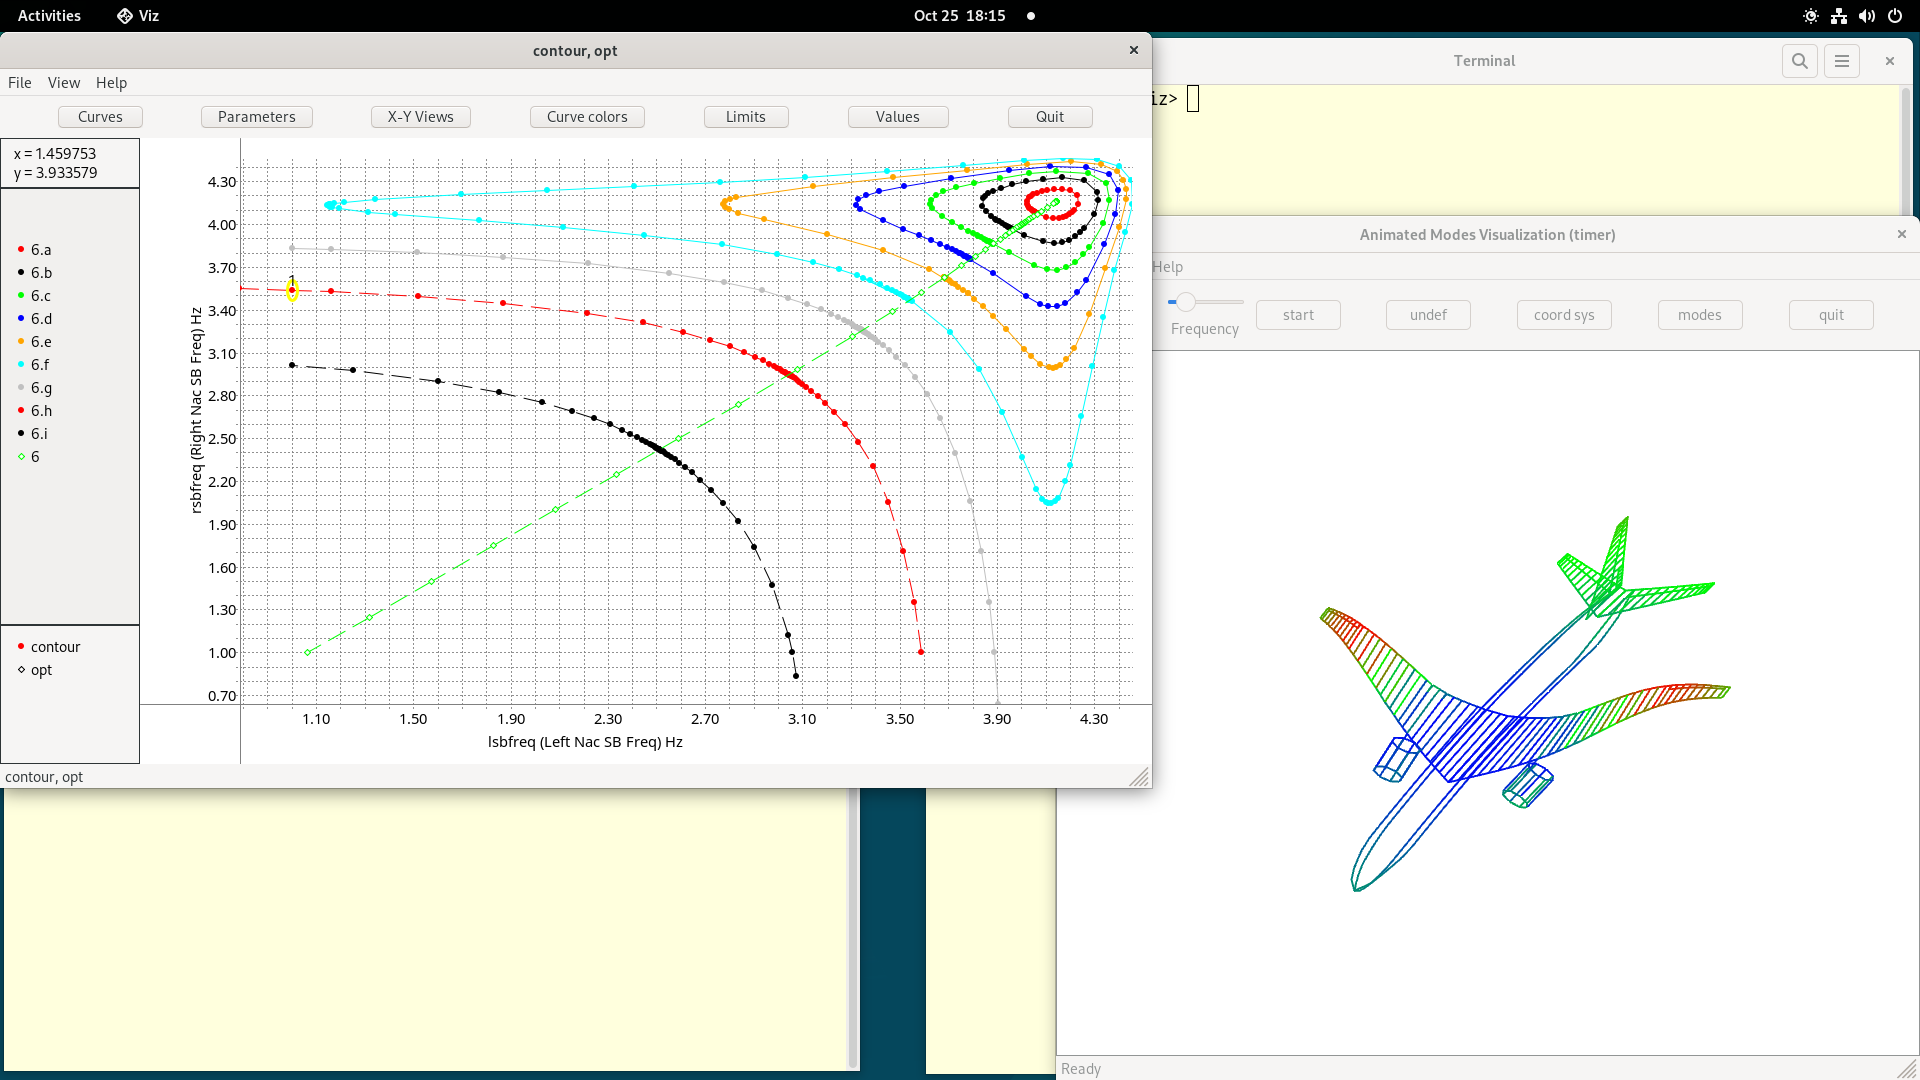
\includegraphics[height=9cm,width=16cm]{viz-amviz.png}
	\centering
\end{figure}
\vspace{2cm}
\Huge{Flaps Users' Manual}

\vspace{1cm}
\large{Version \input{../../Version}}

\vspace{1cm}
\Large{Edward E. Meyer}
\par
\Large{\ttfamily flapsconsulting@gmail.com}
\end{center}

\author{Edward E. Meyer}

\tableofcontents
\listoftables
\listoffigures

\chapter{Introduction}\label{chap:intro}
\Flaps (FLutter Analysis ProgramS), is a collection of programs for doing various
types of linear and nonlinear flutter analyses in the frequency domain.
The intent is to provide efficient means to do the many parameter studies
required to design and certify aircraft.

Throughout the design and certification of aircraft numerous
flutter analyses must be performed to provide a reasonable degree
of confidence that the aircraft is safe to fly.
These tasks include
\begin{enumerate}\label{sect:tasks}
	\item search for neutral-stability,\index{neutral-stability}
			\index{stability!neutral} the boundary between decaying and growing
			oscillations, through the design velocity range;
	      known as \Newterm{flutter speeds}, the lowest such speed
			is sometimes called the \Newterm{critical flutter speed}
			\index{flutter!critical speed}, though it is not always the most
			important.
	\item study the variation in these flutter speeds with various parameters,
	     both design parameters like stiffnesses or control-system
		  equations, and flight parameters like altitude or fuel loading.
	\item determine the effects of including nonlinearities,
			which often limit the amplitude of growing oscillations,
			a phenomenon known as \Newterm{limit-cycle oscillations} or \Lco.
	\item determine the stability of limit cycles:\index{stability!limit-cycle}
	      do small perturbations in amplitude grow or decay to the limit cycle?
	\item each of these tasks usually involves treating from one to hundreds
			of aeroelastic modes
	\item as with any field that involves analyzing lots of data, visualizing
			flutter data is a challenging task
\end{enumerate}

Traditional methods for solving flutter equations
\footnote{An excellent treatment of traditional methods is \cite{demasi2024introduction}}
treat them as some form of eigenvalue problem, requiring approximation and
manipulation of the equations. These methods are incapable of treating
control systems, nonlinearities, or parameter variations, nor can they
provide continuous solution curves.

In contrast, the approach taken here is to consider the flutter equations as a
set of nonlinear equations in several parameters, including the displacements.
This allows for including control systems, nonlinearities, gyroscopics,
and parameter variations, in addition to any of the traditional
formulations.
These parameterized nonlinear equations can be solved very efficiently
over a range of parameters using \Newterm{numerical continuation}
\cite{allgower1990numerical}.

The goal of many traditional methods is to give more accurate estimates
of damping at velocities below the flutter speed to answer the questions:
how quickly will disturbances die out? and how close are we to flutter?
Another goal is to find so-called \emph{matched-point}\index{matched point}
solutions, where the Mach number used to compute the aerodynamics is correct,
usually requiring iteration. Both of these goals are easily satisfied in \Flaps.

Because parameters are so important to flutter analysis \Flaps has
a variety of ways to introduce new parameters, and to
\Newterm{parameterize matrices} (make them functions of parameters).
Nearly arbitrary combinations of parameters may be used to produce
the curves that are the principle output from \Flaps.
% To ensure all curves produced are continuous (no need to ``connect the dots'')
% two numerical techniques are used: \Newterm{numerical continuation} together
% with a technique called \Newterm{automatic differentiation}.


\subsection{Flaps Capabilities}
% \subsubsection{\Flaps Capabilities}
The application programs comprising Flaps fall into the following
general categories:

\subsubsection{Model building}
\Flaps model building capabilities are intended for education
and research, lacking many of the features of more sophisticated
tools like \Nastran.
The \Cmd{fem} command allows for simple beam modeling,
doublet-lattice unsteady aerodynamics, propeller unsteady
aerodynamics, and gyroscopics. Some of the example problems (\Sectref{chap:examples})
use models built with \Cmd{fem}.

\subsubsection{Importing Data}
More sophisticated models may be imported using a variety of
data formats with the \Cmd{import} command (\Sectref{ref:import}).
        
\subsubsection{Parameterization}
An important aspect of Flaps is it's ability to do parameter
studies. The key to parameter studies is the ability to
define parameters and to create matrices which are functions of
these parameters. Several types of matrix parameterization are available
with the \Cmd{pz} command (\Sectref{ref:pz}),
including multivariate interpolation,
rational-function approximation, 
replacing matrix elements with arbitrary equations,
and the most general: custom evaluation function parameterization.
        
\subsubsection{Data Manipulation}
The \Flaps \Cmd{octlab} command (\Sectref{ref:octlab}) provides means
to perform a variety of matrix manipulations and computations with
\Flaps matrices using either \Matlab\ (www.mathworks.com)
\index{matlab@\Matlab}
or the open-source alternative Octave (octave.org), hence
the name \Cmd{octlab}.
Several of the example problems (\Chapref{chap:examples})
demonstrate this capability.
        
\subsubsection{Flutter}
The {\Cmd{flut} command solves linear flutter equations
in the frequency domain for neutral stability and parameter
variations.
Nonlinearities may be included using the describing-function
technique (\Sectref{sect:desc-fun}, \Sectref{opt:matrix-element}).
        
\subsubsection{Visualization}
Several types of visualization are useful in flutter analyses,
the most common are 2D plots of flutter results;
others include animations of a structure vibrating, plots of
parameterized matrices and interactive display of matrices.
These are treated in the \Cmd{viz} command \Sectref{ref:viz}.

% using the \Cmd{vz} command \Sectref{ref:vz} to create plots
% of flutter data from the \Cmd{flut} command \Sectref{ref:flut}.

% Animations of the structure vibrating or fluttering can be visualized
% with the \Cmd{amvz} command \Sectref{ref:amvz}. Conditions determined
% by parameter values can be selected by clicking on curves from the
% \Cmd{vz} command \Sectref{sect:animation}.
% Results from \Cmd{flut} can be plotted in 2D or 3D using
% the \Code{vz} command (\Sectref{ref:vz}); if nodal and modal data are
% available, animated modes can be visualized by selecting points from a \Code{vz} plot.
% The \Flaps \Cmd{vz} command
% may also be used on the command-line with any plotfile from \Cmd{flut}.
% see the \Cmd{vz} reference (\Sectref{ref:vz}) for more details.

% Matrices, unless they are very small, are difficult to examine on
% the printed page so \Flaps displays them graphically in a way that
% allows interactive examination of elements.
% The \Cmd{display} command (\Sectref{ref:display})
% is the primary way to visualize matrices.

\subsection{Overview}
This manual consists of the following chapters:

\begin{description}
	\item[\ref{chap:theory} Solving Flutter Equations]
	Frequency-domain linear and nonlinear flutter equations and
	the techniques used to solve them

	\item[\ref{chap:parameters} Parameters]
	describes builtin parameters and how to define and use new parameters

	\item[\ref{chap:equations} Equations]
	describes how and where equations are used in \Flaps and
	how to create and assign equations

	\item[\ref{chap:functions} Functions]
	explains how to write functions to modify or create matrices

	\item[\ref{chap:visualization} Visualization]
	2D plotting and animated modes

	\item[\ref{chap:commands} Flaps Commands]
	lists specs for each of the \Flaps commands

	\item[\ref{chap:examples} Example Problems]
	describes a few demonstration problems

	\item[\ref{chap:appendices} Appendices]
	gives various details regarding \Flaps commands
                
\end{description}
        
\subsection{System requirements}
Currently \Flaps only runs on Unix and Linux operating systems
(more accurately GNU/Linux). Example problems (\Chapref{chap:examples}),
some of which are of ``real-world'' size, run well on even moderately
powerful PCs.
Flutter analyses run in \Flaps will use the multiple cores available
in most modern cpus to speed up the execution, with each aeroelastic
mode tracked in a separate thread.
% Work is ongoing to extend this to the multiple cores available
% in graphics cards (gpus).
\Flaps is written in \Cpp and in order to use some of the more advanced
features a \Cpp compiler is necessary and a rudimentary knowledge of
the language.

\subsection{Conventions}
Throughout this document the following typographic conventions
are used to (hopefully) make it more readable:

% XXX check that these fonts are what are actually used, e.g. for Cmd
\begin{description}
	\item[\Newterm{italic}]
		is used to highlight new terms and concepts
		when they are first used
                
	\item[\Code{typewriter}]
	is used for computer output or listing of computer files
                
	\item[\Subst{italic typewriter}]
		indicates a parameter which the user should substitute with an
		actual parameter; for example
			\Cmd{flaps} \Subst{filename\/}
     means that the user is to substitute her own file name for
	\Subst{filename\/}
                
	\item[\Cmd{Sans Serif}]
	is used for a computer command or the name of a program,
	for example \Cmd{flaps}
                
	\item[\UserIn{Bold Sans Serif}]
	indicates something typed by the user; for example
	\Code{Login:}\UserIn{jimbob}
                
	\item[$\Matrix{M}$,$\Vector{v}$] 
	Matrices and vectors are printed in bold, with matrices in upper
	case and vectors in lower case.
                
\end{description}}

% \subsection{Getting Started}
Throughout this document we assume the reader has a rudimentary
knowledge of the Linux (Unix) operating system, and is familiar with
terms like environment variable, directories, and can
use an editor such as {\sffamily vi} or {\sffamily emacs}.

% \subsubsection{The \Cmd{flaps} Command}
The basic program used in running Flaps is named \Cmd{flaps}
which should be in your default \Code{PATH}.
While the most common use of \Cmd{flaps} is for processing
files of Flaps commands, \Cmd{flaps} has other options
(see \Sectref{ref:flaps} for more details).

\subsection{Quick Start Guide}
\par
A quick way to get started is to look at some of the
Flaps example files (\Chapref{chap:examples}) and
modify them to suit your purposes. All files ending
with \Code{.fp} are example input files.  You can copy them to
your own directory to modify and run them by typing,
for example (\$ is the default Unix command prompt):
\par
\Code{
\$ flaps contour >out 2>err
}

Note that \Cmd{flaps} assumes a default file extension of \Cmd{.fp}
so it is not necessary to include it.
In this example, output has been redirected to a file named
\Cmd{out} and the standard error listing has been
redirected to a file named \Cmd{err}.
\par
Like the rest of \Flaps, this manual is a work in progress;
it is known to be incomplet, inkorrect, and badly
forma\rotatebox{10}{t}\raisebox{-.2ex}{t}ed.
The author would appreciate comments, criticisms, and corrections.

\newpage
\chapter{Solving Flutter Equations}\label{chap:theory}
A general formulation of the flutter equation includes
gyroscopics, \index{gyroscopics}
viscous damping, \index{damping!viscous}
control-system, Mach and complex reduced-frequency
based unsteady aerodynamics, quasi-linear approximated structural
nonlinearities, and parameterized matrices.  Solving the flutter equation
usually involves a search for neutral stability points, the boundary
between stability and instability, followed by variations in the neutral
stability point with various parameters.  A technique for  solving the
flutter equation under these conditions must be capable
of solving systems of nonlinear parameterized equations over a range
of parameter values while keeping continuity in all the parameters.
Numerical continuation methods\index{continuation!method}
\cite{rheinboldt1986numerical,allgower1990numerical}
are specifically designed
for solving such problems.  A continuation method is presented that is
capable of solving general formulations of the flutter equation for
neutral stability, parameter variations, optimization, model tuning,
and describing function flutter analyses, including an efficient technique for
assessing limit cycle stability.

\section{Flutter Equations}\label{sect:flutter-eqns}

\subsection{Nomenclature}\label{sect:nomenclature}
\index{nomenclature}
\noindent\begin{longtable}{@{}lcl@{}}
% \noindent\begin{tabular}{@{}lcl@{}}
$a$ & & sonic velocity \\
$b$ & & reference length for reduced frequency (usually 1)\index{=b@$b$ (ref. length)} \\
$\mathbb{C}^n$, $\mathbb{C}^{m \times n}$ & & the complex $n$-vectors
   and $m$ by $n$ matrices \\
$\Matrix{D}$ & & complex ($n_e,n_e$) dynamic matrix (\Eqn{eqn:flut} \\
$d$ & & structural damping coefficient \\
$\Vector{f}$ & & vector of $n$ real, nonlinear equations \\
$\Matrix{J}$ & & Jacobian matrix of partial derivatives (\Eqn{eqn:fxprime}) \\
$\Matrix{J}_{i:}$\boldmath{,} $\Matrix{J}_{:j}$ & & row $i$
   and column $j$ of matrix $\Matrix{J}$ \\
$\Matrix{M}$\boldmath{,} $\Matrix{K}$\boldmath{,} $\Matrix{G}$\boldmath{,} &  & mass,
   stiffness, gyroscopic, viscous damping, \\
$\Matrix{V}$, $\Matrix{A}$, $\Matrix{T}$ & & unsteady aero and
   user-defined matrices (\Eqn{eqn:flut}) \\
$M$ & & $V/a$, Mach number \\
$n_e$ & & the number of complex generalized coordinates (\Gc) \\
$q$ & & $\rho V^2/2$, dynamic pressure \\
$\Vector{q}$ & & complex generalized coordinates (\Gc) (\Eqn{eqn:eta-def}) \\
$\Vector{\chi}$ & & real vector of physical motion of the structure
	at discrete points (\Eqn{eqn:motion}) \\
$\Matrix{Q}$, $\Matrix{R}$ & & QR factors of the transposed Jacobian (\Eqn{eqn:qr}) \\
$\mathbb{R}^n$, $\mathbb{R}^{m \times n}$ & & the real $n$-vectors and $m$ by $n$ matrices \\
$\Re(), \Im()$ & & real and imaginary parts of a complex variable \\
$s$ & & Laplace variable $\sigma + i\omega$, aka characteristic exponent \\
$\bar{s}$ & & $sb/V$, complex reduced frequency \\
$\Vector{t}$ & & tangent vector \\
$V$ & & velocity (true airspeed) \\
$\Vector{w}$ & & projection vector (\Eqn{eqn:project}) \\
$\Vector{x}$ & & independent variables \\
$\Vector{x}_j^i$ & & $i\text{th}$ corrector iteration at the $j\text{th}$
   continuation step (\Eqn{eqn:predictor}) \\
$x_i$ & & $i\text{th}$ element of vector $\Vector{x}$ \\
$\Vector{y}$ & & complex eigenvector (\Eqn{eqn:flut}) \\
$z$ & & geometric altitude \\
$\delta$ & & freeplay gap or bilinear stiffness breakpoint (\Eqna{eqn:gap}{eqn:bilinear}) \\
$\eta$ & & 2-norm of the generalized coordinates (\Gc) (\Eqn{eqn:eta-def}) \\
$\gamma$ & & normalized amplitude (\Eqna{eqn:gap}{eqn:bilinear}) \\
$\omega$ & & oscillation frequency (imaginary part of the complex frequency) \\
$\bar{\omega}$ & & reduced frequency $\omega b/V$ \\
$\Matrix{\Phi}$ & & transformation from generalized to physical coordinates (\Eqn{eqn:motion}) \\
$\rho$ & & fluid density \\
$\sigma$ & & stability factor aka damping \\
$\bar{\sigma}$ & & reduced stability factor $\sigma b/V$ \\
$\tau$ & & arclength along a curve \\
$\Step$ & & stepsize in the continuation process (\Eqn{eqn:predictor}) \\
$\|\Vector{y}\|_2$ & & 2-norm of vector $\Vector{y} =
   \sqrt{\Vector{y}^T\Vector{y}}$ \index{2-norm}\\
$()^T$ & & transpose \\
$(\;)^*$ & & conjugate transpose \\
% \Code{code} & & name of a website, computer code variable, or subroutine
% \end{tabular}
\end{longtable}

\subsection{Linear Flutter Equations}\label{sect:linearflutter}
Flutter equations in the frequency domain are based on
the assumption that the physical motion of the structure at discrete points
($\Vector{\chi}$) as a function of time
is related to a set of complex generalized coordinates (\Gc)
$\Vector{q}$ by complex exponentials
\begin{equation}
\Vector{\chi}(t) = \Re(\Vector{q}e^{st})
\end{equation}
or more commonly, by modal-reduction\index{modal reduction} generalized coordinates:
\begin{eqnarray} % eqn:motion
\label{eqn:motion}
\Vector{\chi}(t) & = & \Re \left(\Matrix{\Phi}\Vector{q}e^{st}\right) \nonumber \\
              & = & \Re \left[\Matrix{\Phi}\Vector{q} e^{\sigma t}
				  			\left(\cos \omega t + i \sin \omega t \right) \right]
\end{eqnarray}
where $\Matrix{\Phi}$ \index{=Phi@$\Matrix{\Phi}$!modal reduction} is typically
a matrix of vibration modes and component modes \cite{craig1968coupling},
$t$ is time, $s = \sigma + i\omega$ is the complex frequency, $\omega$
is the frequency and oscillations are growing, neutral or decaying if the
\Newterm{stability factor} $\sigma$ is positive, zero or negative, respectively.
It is useful, especially when dealing with nonlinear flutter,
\index{nonlinear flutter} to express the flutter equations in terms of an
eigenvector $\Vector{y}$ which always has unit 2-norm and one component real:
\begin{equation}\label{eqn:normal}
\|\Vector{y}\|_2 = \sqrt{\Vector{y}^*\Vector{y}} = 1,
\hspace{0.1in}
\Im(y_k) = 0
\end{equation}

The generalized coordinates are related to the eigenvector by a real scale
factor:
\begin{equation}\label{eqn:eta-def}
\Vector{q} = \eta \Vector{y}
\end{equation}
\index{g.c.!norm}\index{=eta@$\eta$ (\Gc norm)}
where $\eta$ is the 2-norm of the \Gc;
so whereas $\Vector{y}$ always has unit norm, the norm of $\Vector{q}$ 
is controlled by $\eta$.

A general set of flutter equations in the frequency domain
can be written as
\begin{equation}\label{eqn:flut}
\left[ s^2 \Matrix{M} + s \Omega\Matrix{G} + s \Matrix{V} +
 (1 + id) \Matrix{K} - q \Matrix{A} (\bar{s},M) + \Matrix{T} \right]
  \Vector{y} = \Matrix{D}\Vector{y} =
  \Vector{0} \; \; \in \mathbb{C}^{n_e},
\end{equation}
where
$\Matrix{M}$, $\Matrix{K}$, $\Matrix{G}$, $\Matrix{V}$, and $\Matrix{A}$
are the ($n_e,n_e$) mass, stiffness, gyroscopic, viscous damping, and
unsteady aerodynamic matrices, respectively,
$\Matrix{T}$ is a user-defined matrix (e.g. control-system equations),
$d$ is the structural damping coefficient,
$q = \rho V^2/2$ is the dynamic pressure,
$\bar{s} = sb/V = \bar{\sigma} + i\bar{\omega}$ is the complex reduced frequency,
$b$ is a characteristic length, usually a semi-chord,
$V$ is the free-stream velocity,
$M = V/a$ is the free-stream Mach number,
$a$ is the sonic velocity, and
$\Matrix{D}$ is the complex dynamic matrix.

If none of the matrices in \Eqn{eqn:flut} are functions of the generalized
coordinates they are referred to as \Newterm{linear flutter} equations,
in spite of the fact that they are nonlinear functions of reduced frequency
and possibly others.

\subsection{Nonlinear Flutter Equations}\label{sect:lco}
If any of the matrices are functions of the generalized coordinates
\Eqn{eqn:flut} is referred to as a \Newterm{nonlinear flutter} equation.
The actual motion in a nonlinear frequency domain flutter analysis 
does not in general follow the assumption \ref{eqn:motion}; retaining this
assumption results in an a
\Newterm{quasi-linear approximation} \cite{gelb1968multiple}.
Describing~functions and harmonic balance methods
are examples of quasi-linear approximations.
Rather than calling flutter analyses that use such approximations
nonlinear, perhaps they should be called \Newterm{quasi-linear flutter}.

The extra parameter $\eta$ (\Eqn{eqn:eta-def}) complicates nonlinear
flutter solutions primarily in the fact that they can exhibit \Newterm{LCO},
\index{limit cycle oscillations|see{LCO}} oscillations with $\sigma=0$
at an amplitude $\eta \ge 0$. In addition, an LCO can be stable or unstable;
given a small increase (decrease) in amplitude, if $\sigma$ goes
negative (positive) it is stable and the amplitude will decrease
(increase) to the LCO. On the other hand, if $\sigma$ goes positive
(negative) it is unstable and the amplitude will continue to increase
(decrease) until it encounters a stable LCO.
Stability of limit cycles therefore depends upon the sign of
$\partial \sigma/\partial \eta$.\index{LCO!stability of}
% $\frac{\partial \sigma}{\partial \eta}$.
\par
Another complication with nonlinear equations is
\Newterm{latent LCO}\index{LCO!latent} \cite{meyer2021latent},
latent in the sense that they are difficult to find
because they may appear over a narrow range of amplitudes and
do not appear at zero amplitude, so they do not show up in linear
flutter solutions and may not show up in flight testing.
Some techniques for finding latent LCO will be discussed in
\Sectref{sect:application}.


\subsection{Matrix Parameterizations}\label{sect:pz}
The matrices in \Eqn{eqn:flut} may be functions of various parameters, directly
or indirectly related to the parameters $\Vector{p}$ in \Eqn{eqn:realeqn} by
matrix parameterizations.
The \Flaps \Cmd{pz} command \Sectref{ref:pz} provides several ways to
parameterize matrices, including
\begin{itemize}
\item assigning an arbitrary equation to a matrix element
\item interpolating a set of matrices with respect to 1, 2, or 3 parameters
\item modifying an existing matrix or creating a new matrix
      with a custom function (\Chapref{chap:functions})
\end{itemize}

\subparagraph{Matrix element equations} are the simplest way
to parameterize a matrix. The \Cmd{pz} (\Sectref{ref:pz}) command allows assigning
an equation (\Chapref{chap:equations}) to a matrix element,
for example a stiffness matrix might be given the equation
\begin{lstlisting}
[3,3] *= freeplay(0.05, 3)
\end{lstlisting}
which multiplies the $(3,3)$ diagonal of the matrix by the value
returned by builtin function \Code{freeplay} to give
the equivalent stiffness according to the amplitude of dof 3.
Equations may contain parameter names, constants, and builtin
standard math functions like \Code{sin}, \Code{cos}, etc,
the same as when defining new parameters (\Sectref{sect:newpar}).

\subparagraph{Interpolation} in 1, 2, or 3 independent variables
requires a set of matrices sufficient to give accurate interpolated
values.
For example, it is common practice to compute
the unsteady aerodynamic matrix $\Matrix{A}$ at several values of
reduced frequency \Code{rf} (and possibly reduced stability factor
\Code{rsf} and Mach number) and interpolate to get the
intermediate values necessary for continuation. The aerodynamic matrix is
then indirectly dependent on velocity and frequency.
\index{aerodynamics!interpolation}

Another common interpolation is to make the mass matrix a function
of the amount of fuel on the aircraft, allowing continuous variations
in fuel loading to demonstrate stability throughout the flight envelope.
This type of parameterization can be done by forming finite-element
mass matrices at several fuel loadings, reducing them using the
$\Phi$ matrix (\Eqn{eqn:motion}), and interpolating with respect to
\index{=Phi@$\Matrix{\Phi}$!parameterizing with}
fuel percent.

\subparagraph{Custom evaluation functions}\index{function!custom} are a
powerful way to parameterize a matrix either to generate a new matrix
or modify an existing matrix,
but require caution and some programming experience (\Chapref{chap:functions}).
\index{custom function!matrix parameterization}
A matrix modified in this manner can be an almost arbitrary function
of parameters. The main restrictions are: 1) functions must be written in \Cpp;
and 2) the function must have a specific argument list and return value.
For example, a small function that modifies the (1,1) term of a stiffness matrix
\begin{lstlisting}
int mystif(pset& ps, int nr, int nc, complex<Ad>& ca) {
   Ad gap = ps.parval("gap");
   int dof{1};
   ca[IJ(dof-1,dof-1,nr)] *= df::freeplay(ps, gap, dof);
   return 0;
}
\end{lstlisting}
where \Code{pset} is the current set of parameters, builtin and user-defined,
\Code{parval} is a function that returns the current value of its
string argument, in this case the user-defined parameter \Code{gap},
\Code{df::freeplay} is a builtin function which returns a factor between
zero and 1 that accounts for the current amplitude of \Code{dof},
and \Code{nr} and \Code{nc} are the dimensions of the complex
automatic differentiation matrix \Code{ca}.\index{automatic differentiation}
Note two differences between the use of builtin function \Code{freeplay}
here and in equations (\Sectref{sect:eqn-df}): here \Code{freeplay} is
in namespace \Code{df} so it must be prefixed with \Code{df::}, and
it has an additional argument, the set of parameters \Code{ps}.

\subparagraph{Control-system equations}
\index{control systems}
can be implemented by writing a custom function
\index{custom function!control-system}
\index{function!custom}
with the control-system equations
and using it to parameterize a new matrix in
\Cmd{pz} (\Sectref{ref:pz}) which is then used in \Cmd{flut} as matrix $\Matrix{T}$.

The control-system matrix usually has more rows and columns than the
mass matrix. The extra rows and columns correspond to control-system
degrees of freedom. $\Matrix{T}$ typically has the form:
\begin{equation}
\Matrix{T} = \left[ \begin{array}{cc}
			\Matrix{T}_{11}     &   \Matrix{T}_{12} \\
	      \Matrix{T}_{21}     &   \Matrix{T}_{22}
		\end{array} \right]
\end{equation}
where $\Matrix{T}_{11}$ is the size of the mass matrix,
$\Matrix{T}_{21}$ transforms generalized coordinates to physical sensor motions,
$\Matrix{T}_{22}$ contains control-system equations, and $\Matrix{T}_{12}$ provides
feedback to the structure from the control-system degrees of freedom.
The extra control-system degrees of freedom must be accounted for when
forming the dynamic matrix.
\par
The \Cmd{lti} command (\Sectref{ref:lti} creates the $\Matrix{T}$ matrix
from a state-space linear time-invariant (LTI) control system from Simulink;
details of the conversion from a state-space
representation to the frequency-domain $\Matrix{T}$ matrix are in
\Sectref{sect:abcd-conversion}.\index{LTI control system}
\index{ABCD control system|see{LTI control system}}
% If the controls equations are available in linear, time-invariant state
% variable form (\cite{brogan1982modern} p. 172):
% \begin{eqnarray*}
% \dot{\Vector{x}}_c &=& \Matrix{A}\Vector{x}_c + \Matrix{B}\Vector{u} \;\; \in \mathbb{R}^{n_c} \nonumber \\
% \Vector{y} &=& \Matrix{C}\Vector{x}_c + \Matrix{D}_c\Vector{u} \;\; \in \mathbb{R}^{n_o} \nonumber \\
% \end{eqnarray*}
% where $\Vector{u}$ is an $n_i$ vector of inputs, $\Vector{y}$ is an $n_o$ vector of outputs,
% $\Vector{x}_c$ is an $n_c$ vector of state variables,
% and $\Matrix{A}$, $\Matrix{B}$, $\Matrix{C}$, and $\Matrix{D}_c$ are real matrices,
% it can be shown that
% \begin{eqnarray*}
% \Matrix{T}_{11} &=& -\Matrix{KED}_c\Matrix{S} \Matrix{\Phi}_c \nonumber \\
% \Matrix{T}_{12} &=& -\Matrix{KEC}	\nonumber \\
% \Matrix{T}_{21} &=& \Matrix{BS} \Matrix{\Phi}_c \nonumber \\
% \Matrix{T}_{22} &=& \Matrix{A} - s\Matrix{I} \nonumber
% \end{eqnarray*}
% where $\Matrix{\Phi}_c$ are the rows of the transformation matrix corresponding to the
% control system inputs; and $\Matrix{S}$ is a diagonal matrix consisting of either
% 1, $s$, or $s^2$, depending on whether the corresponding input is a displacement,
% velocity, or acceleration.
% $\Matrix{E}$ is a real matrix that transforms the control system output $\Vector{y}$
% to generalized coordinates.

\subsection{Describing functions}\label{sect:desc-fun}\index{describing function}
Describing functions are a type of quasi-linear approximation to a
nonlinear function. Such an approximation is {\em quasi}-linear because
although they are functions of the amplitude of oscillation, the 
form of the nonlinear function in the time domain matches the
assumption of \Eqn{eqn:motion}, allowing for solutions with linear
flutter codes.

Two ways of thinking about describing functions are
\begin{enumerate}
	\item as a projection of a nonlinear function onto $\sin \omega t$
	\item as the fundamental harmonic term in the Fourier series
			expansion of the function
\end{enumerate}

An analytic expression can be derived for
many types of nonlinearities by evaluating the projection integral
\begin{equation}\label{eqn:df-defn}
f_{p} (t) = \frac{\omega}{\pi} \sin \omega t
	\int_{0}^{2\pi/\omega} f(q_j \sin \omega t) \sin \omega t dt
\end{equation}
where $q_j$ is the oscillation amplitude, $f(t)$ is the nonlinear force,
and $f_p$ is the linear approximation.

Two nonlinearities that are important for flutter are \Newterm{freeplay},
(or \Newterm{gap} or \Newterm{dead zone}),
which is always present in control surfaces, and bilinear stiffness,
which affects wing-mounted engines.
The force-displacement curve and its describing function approximation
for freeplay are shown in \Figref{fig:gap-force}.
\begin{figure}[ht] 	% complains if h
%		\includegraphics[height=2.5in,width=3.2in]{gap-force.pdf}
		\includegraphics[height=2.5in,width=3.2in]{gap-force.eps}
	\centering
	\caption{Describing Function Approximation of Freeplay}\label{fig:gap-force}
\end{figure}
Evaluating the integral leads to
% \begin{equation}
% c(q_k,\delta)  =
% 	\begin{cases}
% 		\frac{1}{\pi} \left[ \pi - 2 \sin^{-1}(1/\gamma) - \sin(2\sin^{-1}(1/\gamma)) \right] & \text{if} \gamma = \left|q_k\right|/\delta \geq 1 \\
% 		0 & \text{otherwise}
% 	\end{cases}
% \end{equation}
\begin{eqnarray}
\label{eqn:gap}
c_j(\gamma_j)  & = &
	\begin{cases}
		1 - (\xi + \sin{\xi})/\pi &
			\text{if} \; q_j/\delta_j > 1 \nonumber \\
		0 & \text{otherwise}
	\end{cases} \\
	\xi & = & 2\sin^{-1}(\delta_j/q_j)
\end{eqnarray}
for a gap $\delta_j$. Another common nonlinearity is bilinearity,
illustrated in \Figref{fig:bilinear-force}.
\begin{figure}[!ht]	% complains if !h
%		\includegraphics[height=2.5in,width=3.2in]{bilinear-force.pdf}
		\includegraphics[height=2.5in,width=3.2in]{bilinear-force.eps}
	\centering
	\caption{Describing Function Approximation of Bilinear Force}\label{fig:bilinear-force}
\end{figure}
with describing function
% represents a bilinear element with $r$ the ratio of stiffnesses above and
% below $\delta_j$, the diagonal is multiplied by

\begin{eqnarray}
\label{eqn:bilinear}
b_j(\gamma_j,r_j) & = &
	\begin{cases}
		r_j + \frac{2}{\pi} (1 - r_j) \left[ \xi + \gamma_j^{-2} \sqrt{\gamma_j^2 - 1} \right] & \text{if} \; \gamma_j = |q_j|/\delta \ge 1 \\
		1 & \text{otherwise}
	\end{cases} \\
	\xi & = & \sin^{-1}(1/\gamma_j)
\end{eqnarray}
Figure \ref{fig:df} shows the factors $c$ and $b$; note the transitions
at $\delta$ have been smoothed to avoid numerical problems with the
continuation method.
\begin{figure}[!ht]	% complains if !h
%	\includegraphics[height=2.4in,width=3.2in]{df.pdf}
	\includegraphics[height=2.4in,width=3.2in]{df.eps}
\centering
\caption{Describing functions}\label{fig:df}
\end{figure}

Analytical forms of many other describing functions have been 
derived \cite{gelb1968multiple}; if an appropriate one is not
found, it may be possible to derive the analytical form using
\Eqn{eqn:df-defn}.

\subsubsection{Computing Describing Functions Numerically}
\label{sect:computing-df}
If it is not practical to derive an analytic expression for a
describing function, it could be evaluated numerically by using
a fast Fourier transform and taking the fundamental harmonic.
Repeating this at several oscillation amplitudes (and possibly
frequency), then interpolating the result.
An experimental framework for doing this requires the user to supply
3 functions either as an input file section \Sectref{sect:input-file} or
in a file. These functions are compiled automatically at the beginning
of a \Flaps job, and run to create a set of interpolation coefficients
giving the describing function as a function of specified generalized
coordinate amplitudes. The user then applies the describing function
to a matrix by calling a \Flaps function, \Code{dfval}, either in
a matrix-element equation or a custom evaluation function.
More details are in \Sectref{sect:df-approx}.

\subsection{Choosing a Solution Technique}\label{sect:soln-req}\index{solution requirements}
Considering the tasks in \Sectref{sect:tasks} and the fact that the equations
are a system of nonlinear parameterized equations it is clear that the solution
technique must be capable of tracing curves over a range of parameters
while maintaining continuity between points on the curve.
In addition, because there are usually multiple modes to trace, tracing them
in parallel is very desirable.
Also worth considering is how comprehensible is a method to the average user;
a solution technique that reformulates the equations to fit techniques from
another discipline might be less desirable than one that uses familiar equations
and methods.

The class of methods known as numerical continuation fulfills these requirements very well.
% has been developed to do just that.
There are two broad categories of numerical continuation:
piecewise linear and predictor-corrector, the latter requires differentiability,
the former does not. By exploiting differentiability, predictor-corrector
continuation methods are more robust and efficient than piecewise-linear, so
that is what is used here.

For predictor-corrector methods it is necessary to have available
accurate derivatives of all elements of \Eqn{eqn:flut}. Automatic differentiation
\index{automatic differentiation!justification}
is a programming technique that gives derivatives of chosen parameters
as the flutter equation is evaluated, avoiding the need for coding derivatives
and the risk of coding errors; and because it gives exact derivatives it
avoids the approximation (and expense) associated with finite differencing.
Automatic differentiation is used extensively in \Flaps, both for parameter
and for matrix derivatives.

\newpage
\section{Numerical Continuation}\label{sect:continuation}
\index{continuation!method}
\subsection{Background}
Numerical continuation has been developed since the middle of the
20th century as a means of solving systems of nonlinear equations that
are dependent on one or more parameters. For example, 
the buckling of a beam in compression can be modeled as a set of
nonlinear equations dependent on the compression loading; methods for
solving these problems, known as incremental methods,
were some of the earliest continuation methods.
At the same time similar techniques were being developed to solve
so-called \Newterm{homotopy} problems where an approximation to a set
of nonlinear equations is incrementally adjusted to lead to the true
solution (\Sectref{sect:homotopy}).
As with finite-elements these methods, which were largely
invented by engineers, were put on solid theoretical footing by
mathematicians, making them more abstract and more accessible to other
fields. Mathematicians who have contributed to the development of
numerical continuation include
\cite{allgower1990numerical,
keller1987lectures,
rheinboldt1981numerical,
rheinboldt1983locally,
rheinboldt1983algorithm,rheinboldt1986numerical}.

Modern numerical continuation is a class of techniques for solving
underdetermined systems of nonlinear equations:
\begin{eqnarray}\label{eqn:fx}
\Vector{f}(\Vector{x}) = \Vector{0} & \in & \mathbb{R}^{m} \nonumber \\
\Vector{x} & \in & \mathbb{R}^{n}
\end{eqnarray}
where the number of equations $m$
is fewer than the number of independent variables $n$.
Because there are fewer equations than unknowns, there are an infinite
number of solutions.
Depending on the difference $n-m$, the solution space consists of
curves ($n-m = 1$), surfaces ($n-m = 2$), and so on; the main focus here
is on curves, but an optimization procedure (\Sectref{sect:optim}
uses higher dimensions.
\par
Numerical continuation is ideally suited for solving systems of equations
like \Eqn{eqn:realeqn}; moreover, they solve the system of equations
so that solutions form continuous curves,
an important consideration for the solution of flutter equations
where aeroelastic modes often become close, making them difficult to
keep separated.
\par
There are a variety of predictor-corrector continuation methods, 
reminiscent of ordinary differential equation solvers.
Many methods
(\cite{cardani1978continuation}, \cite{yu2020nonlinear},
\cite{allgower1990numerical} p. 3),
choose a particular parameter to increment throughout the tracing of curves,
but these methods can fail if the curve has \Newterm{limit points} in
the continuation parameter.
A limit point is where a curve reaches a minimum or maximum in a parameter,
and the tangent to the curve has a zero component for that parameter,
so that incrementing that parameter does not increment the distance along the
curve.
Locally parameterized continuation methods \cite{rheinboldt1983locally}
avoid this problem\index{continuation!locally parameterized}
by choosing the best parameter to increment at each point.
These methods constrain the corrector steps to be at constant values of the
continuation parameter.
Instead, so-called pseudo-arclength methods take steps along the tangent
to the curve, avoiding the problem with limit points and the complexity of
choosing locally optimal continuation parameters.
% A pseudo-arclength method can constrain the corrector steps to be perpendicular
% to the tangent, or use a minimum-norm corrector; both methods will be presented here.

\subsection{Pseudo-Arclength Continuation}\label{sect:pseudo}
\index{continuation!pseudo-arclength}
This method takes steps along the curve in terms of the arclength ($\tau$),
unlike many other continuation methods that take steps in terms of
one of the parameters. The fact that these are finite-size steps makes them
approximations to the arclength, hence the name pseudo-arclength.
% Taking steps in terms of a parameter can lead
% to trouble if the curve comes to a point where the parameter is
% changing very little or not at all; these \Newterm{limit points} cause
% no trouble for a pseudo-arclength method because the metric for steps
% is always based on distance along the curve, not an individual variable.
\par

Some characteristics of the method can be shown by differentiation
with respect to the arclength $\tau$; first note that
\begin{equation}
d\tau = ||d\Vector{x}||_2 = \sqrt{d\Vector{x}^Td\Vector{x}}
\end{equation}
Then the derivative of $\Vector{x}$ with respect to $\tau$ is the
tangent to the curve:\index{tangent}
\begin{equation}\label{eqn:t-properties}
\frac{d\Vector{x}}{d\tau} = \dot{\Vector{x}} =
 	\frac{d\Vector{x}}{\sqrt{d\Vector{x}^T d\Vector{x}}} = \Vector{t}
\end{equation}
which shows that the tangent has unit length: $\Vector{t}^T\Vector{t} = 1$.
Taking the derivative of \Eqn{eqn:fx} with respect to $\tau$,
\begin{equation}\label{eqn:fxprime}
\Vector{f}'(\Vector{x})\dot{\Vector{x}} =
	\left[\frac{\partial f_i}{\partial x_j}\right]\frac{d\Vector{x}}{d\tau}
	= \Matrix{J}\Vector{t} = \Vector{0}
\end{equation}
shows that the tangent is a null vector of the Jacobian matrix ($\Matrix{J}$).
\index{Jacobian}\index{matrix!Jacobian}

% Fundamental to continuation methods is the
% Jacobian matrix of partial derivatives of
% $\Vector{f}$ with respect to $\Vector{x}$:
% \index{Jacobian}\index{matrix!Jacobian}

% \begin{equation}\label{eqn:jacobian}
% \Matrix{J}(\Vector{x}) = \Vector{f}'(\Vector{x}) = \left[ \frac{\partial f_i}{\partial x_j} \right] \;\; \in \mathbb{R}^{m \times n}
% \end{equation}
% and a tangent vector $\Vector{t} \in \mathbb{R}^{n}$ with the following properties:
% \begin{eqnarray}
% \label{eqn:t-properties}
% \Matrix{J}\Vector{t} & = & \Vector{0} \nonumber \\
% \Vector{t}^{t}\Vector{t} & = & 1 \nonumber \\
% \Vector{t} & = & \frac{\partial \Vector{x}}{\partial \tau}
% \end{eqnarray}
% where $\tau$ \index{tau@$\tau$} is the arclength along the curve, hence the name pseudo-arclength.
\par
Starting from a known solution $\Vector{x}_0$, a curve is traced through a range
of the parameters.
At step $j+1$, the solution is predicted from the converged solution
at step $j$ and the tangent
\begin{equation}\label{eqn:predictor}
\Vector{x}_{j+1}^{0} = \Vector{x}_{j} + \Step\Vector{t}
\end{equation}
where $\Step$ is the stepsize, which must be chosen carefully.
Too large a step, and the corrector may not converge or may converge
to the wrong root; too small a step means extra work.
Den Heijer and Rheinboldt \cite{denheijer1981steplength}
studied the problem of computing
step sizes, and Rheinboldt \cite{rheinboldt1983locally}
produced a continuation code
using their algorithm, taking in to account the curvature
and the rate and quality of corrector convergence.
No attempt will be made to present the technique; a good summary is given
in \cite{rheinboldt1986numerical}.
\index{continuation!stepsize}

Starting with the prediction $\Vector{x}_{j+1}^0$,
the corrector iterates to find the solution $\Vector{x}_{j+1}$
using a Newton-like method computing corrections
$\Vector{h}^i$ satisfying
\begin{equation}
\label{eqn:newton}
\Matrix{J}(\Vector{x}^{i})\Vector{h}^i = -\Vector{f}(\Vector{x}^{i})
\end{equation}
and setting
\begin{equation}
\Vector{x}^{i+1} = \Vector{x}^{i} + \Vector{h}^i
\end{equation}
Equation \ref{eqn:newton} is an underdetermined linear system that has
an infinity of solutions; the smallest such solution can be computed using
a QR factorization of the transposed Jacobian which splits it into an
orthogonal matrix ($\Matrix{Q}$) times an upper-triangular matrix $\Matrix{R}$:

\begin{equation}
\label{eqn:qr}
\Matrix{J}^{t} = \Matrix{QR} = \left[ \Matrix{Q}_1 \;\; \Matrix{Q}_2 \right]
	\left[ \begin{array}{c}
		\Matrix{R}_1 \\
		\Matrix{0} \\
	\end{array}\right]
\end{equation}

which when substituted into \Eqn{eqn:newton} yields the
minimum-norm solution (\cite{golub2013matrix} \S 5.6.2)
\begin{equation}
\label{eqn:h}
\Vector{h}^i = - \Matrix{Q}_{1} \Matrix{R}_{1}^{-t} \Vector{f}(\Vector{x}^i)
\end{equation}

Corrector iterations continue using \Eqnr{eqn:newton}{eqn:h} until
suitable convergence criteria are met, for example for some absolute
tolerance $\epsilon_{a}$ and relative tolerance $\epsilon_{r}$:
\begin{equation}
\| \Vector{f} \| < \epsilon_{a} \hspace{0.2in} \text{and} \hspace{0.2in} \| \Vector{h} \| < \epsilon_{a} + \epsilon_{r}\| \Vector{x} \|
\end{equation}
\index{convergence}
Because elements of $\Vector{f}$ may vary widely in size, it may be advantageous
to compute separate tolerances for each element; a method for computing such
tolerances is discussed in \Sectref{sect:ecc}.
\par
The ($n,n-m)$ matrix $\Matrix{Q}_2$ in \Eqn{eqn:qr},
a by-product of the QR factorization,
is an orthogonal matrix spanning the \textit{nullspace} of the Jacobian,
meaning
\begin{eqnarray}
\Matrix{Q}_{2}^t\Matrix{Q}_2 & = & \Matrix{I} \;\;  \in \mathbb{R}^{n-m \times n-m} \\
\Matrix{JQ}_2 & = & \Matrix{0} \;\; \in \mathbb{R}^{m \times n-m} \nonumber
\end{eqnarray}
The focus here is with curves where $n-m=1$, so $\Matrix{Q}_2$ is an $n$-vector,
which satisfies the requirements of the tangent \Eqna{eqn:t-properties}{eqn:fxprime},
to within the sign. The sign is determined from the previous
tangent: $\Vector{t}_{j+1} = \sgn(\Vector{t}_j^t \Vector{Q}_2) \Vector{Q}_2$
 

% An arbitrary vector $\Vector{w}$ is projected onto the nullspace with
% \begin{equation}
% \label{eqn:project}
% \bar{\Vector{t}} = \Matrix{Q}_2\Matrix{Q}_2^t\,\Vector{w} \;\; \in \mathbb{R}^n
% \end{equation}
% and normalized with
% $\Vector{t} = \bar{\Vector{t}}/\|\bar{\Vector{t}}\|$
% to satisfy \Eqn{eqn:t-properties}.
% If $\;n = m+1$, $\Matrix{Q}_2$ consists of only one column, the projection only
% determines the sign of the tangent,
% and a logical choice for the vector to project is the tangent at the previous
% continuation step to keep the curve tracking in the right direction.
% For the first step, any vector with the desired sign will do.

\subsection{Homotopy}\label{sect:homotopy}
\index{continuation!homotopy}\index{homotopy}
One of the earliest applications of numerical continuation was solving a system
of $n$ nonlinear equations in $n$ unknowns
$\Vector{g}(\Vector{y})=\Vector{0}$ using a
technique known as a \Newterm{homotopy},
where an initial guess to a solution is continuously deformed to an actual solution.
Given an initial guess $\Vector{y}^0$,
the system of equations can be solved with numerical continuation by adding
a variable $\lambda$:
\begin{equation}
\Vector{x} = \left\{\begin{array}{c}
\Vector{y} \\
\lambda \\
\end{array} \right\} \;\; \in \mathbb{R}^{n+1}
\end{equation}
and let
\begin{equation}\label{eqn:homotopy}
\Vector{f}(\Vector{x}) = \Vector{g}(\Vector{y})
	+ (\lambda - 1)\Vector{g}(\Vector{y}^0) = \Vector{0}
\end{equation}
\Eqn{eqn:homotopy} is in a form where numerical continuation may be used to
trace from $\lambda=0$ to $\lambda=1$, giving the desired solution
$\Vector{g}(\Vector{y}) = \Vector{0}$.
This technique will be used to find start points for the continuation process
in \Sectref{sect:startpts}.

\subsection{Targets}\label{sect:targets}
When tracing a curve it is sometimes desirable to ensure that
certain values are included in the solution.\index{targets}
For example,
points of neutral stability ($\sigma = 0$) are often needed precisely;
parameter limits may need to be reached exactly, and intermediate
parameter values may be necessary to start subsequent continuation processes.
This can be done by monitoring the predictor (\Eqn{eqn:predictor}) and
if it passes a target $\hat{p}$ for some parameter $p$, reduce the stepsize
($\Step$) to give the desired value:
\begin{eqnarray}
\hat{p} & = & p + \Step \frac{\partial p}{\partial \tau}
	= p + \Step\sum_{j=1}^n \frac{\partial p}{\partial x_j}\frac{\partial x_j}{\partial \tau} \nonumber \\
	& = & p + \Step \Vector{c} \Vector{t}  \nonumber \\
\Step & = & \frac{\hat{p} - p}{\Vector{c}\Vector{t}} \nonumber \\
\Vector{c} & = & \left[ \frac{\partial p}{\partial x_j} \right] 
\in \mathbb{R}^{1 \times n+1}
\end{eqnarray}
and add an equation to constrain the corrector to converge ``exactly''
to $\hat{p}$:
\begin{eqnarray}
f_{n+1} & = & p - \hat{p} = 0  \nonumber \\
\frac{\partial f_{n+1}}{\partial x_j} & = & \Matrix{J}_{n+1:} = \frac{\partial p}{\partial x_j}
	= \Vector{c}
\end{eqnarray}
If the parameter $p$ is a component of $\Vector{x}$, $\Vector{c}$ is all zeros
but a $1$ in the element corresponding to the parameter, i.e. a row of the identity matrix.


\subsection{Continuation-Optimization}\label{sect:optim}
Normally, to track curves with numerical continuation the number of unknowns
must be exactly one greater than the number of equations; two greater
yields surfaces, three volumes, and so on. Likewise, the tangent is a
vector for curves, a plane for surfaces, and so on for higher dimensions.
By restricting the tangent to being a vector in the higher dimensional
spaces, it is possible, and useful, to trace a curve.

The idea is simple: with more independent variables ($n > m+1$)
the tangent is a hyper-surface and we want choose the direction on it
which increases (or decreases) one particular independent variable most
rapidly. This is done by projecting a special vector onto the hypersurface:
\begin{equation} \label{eqn:project}
\bar{\Vector{t}} = \Matrix{Q}_2\Matrix{Q}_2^t\,\Vector{w} \;\; \in \mathbb{R}^n
\end{equation}
where $\Vector{w}$ is all zeros but plus or minus 1 in the spot for
the variable to be optimized.
The tangent is just $\bar{\Vector{t}}$ normalized with
$\Vector{t} = \bar{\Vector{t}}/\|\bar{\Vector{t}}\|$

% An arbitrary vector $\Vector{w}$ is projected onto the nullspace with
% \begin{equation}
% \label{eqn:project}
% \bar{\Vector{t}} = \Matrix{Q}_2\Matrix{Q}_2^t\,\Vector{w} \;\; \in \mathbb{R}^n
% \end{equation}
% and normalized with
% $\Vector{t} = \bar{\Vector{t}}/\|\bar{\Vector{t}}\|$
% to satisfy \Eqn{eqn:t-properties}.
% If $\;n = m+1$, $\Matrix{Q}_2$ consists of only one column, the projection only
% determines the sign of the tangent,
% and a logical choice for the vector to project is the tangent at the previous
% continuation step to keep the curve tracking in the right direction.

% The method used to compute the tangent vector (\Eqn{eqn:project})
% allows for this restriction simply by choosing the projected vector $\Vector{w}$.

This technique can be used as a type of unconstrained optimization.
\index{optimization}\index{continuation!optimization}
For example, if we want to increase a flutter speed by changing some parameter values
we could include all the relevant parameters in the solution and choose
the vector $\Vector{w}$ to be all zeros except a $1$ in the element
corresponding to velocity. Computing the tangent with this $\Vector{w}$
then gives a path towards higher velocities with respect to all the
parameters that were included.

Another practical application of this technique is in searching for
start points for contours, illustrated in example problems 
goland.fp and nacpv.fp.
\par
% The dimension of the Jacobian nullspace (columns in $\Matrix{Q}_2$)
% is $n-m$. If this difference is greater than 1, there are
% an infinite number of tangent vectors possible instead of just one,
% which means that there is more freedom to guide the tangent in particular
% directions by choosing the vector, $\Vector{w}$ in \Eqn{eqn:project},
% that is projected onto the nullspace.
% A few examples will illustrate the technique.
\par

\subsection{Bifurcation}\label{sect:bifurcation}
\index{bifurcation}
Bifurcation, where a curve splits in two, is usually associated
with nonlinear equations. Because so-called linear flutter equations
are nonlinear in some parameters such as frequency and velocity
(just not generalized coordinates),
it is possible to encounter bifurcation even with linear flutter
equations \cite{meyer2015continuation}.
Unfortunately, it is not always obvious when a bifurcation
has been passed and only one of the branches is traced, possibly
missing an important branch.
Though rare, the consequences of missing a bifurcation can be
serious, so monitoring for bifurcation is done by default in \Cmd{flut}.
Fortunately, detecting bifurcation
and tracing both branches is inexpensive with this continuation method,
as described in \Sectref{sect:detect-bifurcation}, and demonstrated
in \Sectref{ex:bifurcation}
\index{continuation!bifurcation}

\section{Applying Numerical Continuation}\label{sect:application}
The continuation method detailed in \Sectref{sect:continuation} can be
used to solve the various problems in flutter analysis mentioned in
\Sectref{chap:intro} but first \Eqn{eqn:flut} must be converted
to an equivalent set of real equations.

% \subsection{Equivalent real equations}\label{sect:equiv}
% Real equivalents of complex matrices and vectors are
% \begin{equation}
% \label{eqn:toreal}
% \Matrix{D} = \left[ \begin{array}{cc}
% 			\Re(\hat{D}_{ij})  & -\Im(\hat{D}_{ij}) \\
% 	   \Im(\hat{D}_{ij})  & \Re(\hat{D}_{ij})
% 		\end{array} \right],
% \hspace{0.1in}
% \Vector{y} = \left\{ \begin{array}{c}
% 			\Re(\hat{y}_{i}) \\
% 	   \Im(\hat{y}_{i})
% 		\end{array} \right\},
% \hspace{0.1in}
% \end{equation}
The equivalent real representation of a complex n-vector $\Vector{z}$
is just
\begin{equation}
\Vector{z} \Leftrightarrow \left\{ \begin{array}{c}
			\Re(z_{i}) \\
	   \Im(z_{i})
		\end{array} \right\} \;\; i=1,n
\end{equation}
so there is no change to the elements in computer memory, only
a change in declaration from n-complex to 2n-real.

The equivalent real equations to be solved are
\begin{eqnarray}\label{eqn:realeqn}
\left\{\begin{array}{c}
	\Vector{Dy} \\
	\Vector{y}^*\Vector{y} - 1 \\
	y_{2k} \\
\end{array} \right\} & \Leftrightarrow & \Vector{f}(\Vector{x}) = \Vector{0} \hspace{0.2in} \in \mathbb{R}^{2n_e+2} \nonumber \\
\left\{\begin{array}{c}
\Vector{y} \\
\Vector{p} \\
\end{array} \right\} & \Leftrightarrow & \Vector{x} \hspace{0.2in} \in \mathbb{R}^{2n_e+n_p}
\end{eqnarray}
where $\Vector{p}$ is a $n_p$-vector of (usually 3) independent
real parameters which determine what type of analysis is to be performed,
as detailed in \Sectref{sect:soln-types}.

\subsection{Types of Solution}\label{sect:soln-types}
The continuation method discussed in \Sectref{sect:pseudo}
is used to solve \Eqn{eqn:realeqn}.
Many possibilities exist for the type of solution, depending upon the
choice of the independent parameters $\Vector{p}$, matrix parameterizations,
and nonlinearities. Several of the more common types of solution are
listed here; the hope is that they will inspire other useful types.

\subparagraph{Linear flutter equations}\label{sect:app-linear}
are when none of the matrices in \Eqn{eqn:flut} are functions of
the generalized coordinates (\Eqn{eqn:eta-def}.
To illustrate some of the most common types of linear flutter solution
combinations of 5 parameters will be used:
$\sigma$, $\omega$, $V$, $p_1$, and $p_2$.  where $p_1$ and $p_2$
are arbitrary parameters like stiffnesses or masses.
Many other combinations are possible, for example
$d$, $\omega$, $V$ is a traditional V-g solution.

\begin{equation}\label{eqn:combinations}
\begin{array}{lclll}
\Vector{p} & = &
	\left\{ \begin{array}{c}
		V \\
		\sigma \\
		\omega
	\end{array}\right\}, \;\; & p_1, p_2 \;\;\text{constant}: & \hspace{0.1in} \text{vso} \\[0.3in]
	  & = & 
	\left\{ \begin{array}{c}
		V \\
		\omega \\
		p_1
	\end{array}\right\}, \;\; & p_2 \;\;\text{constant}: & \hspace{0.1in} \text{vop} \\[0.3in]
	  & = & 
	\left\{ \begin{array}{c}
		\omega \\
		p_1 \\
		p_2
	\end{array}\right\}, \;\; & V \;\;\text{constant}: & \hspace{0.1in} \text{contour} \\[0.3in]
\end{array}
\end{equation}
Each type of analysis has been given an acronym: vso \index{vso} is a traditional
flutter analysis where the goal is to find neutral stability\index{stability!neutral}
($\sigma = 0$) points; vop\index{vop} is a parameter-variation where the variation
in flutter speed with a parameter ($p_1$) is sought. Varying 2 parameters, $p_1$ and
$p_2$ and $\omega$ (opp\index{opp}) gives constant-velocity contours.

\subparagraph{Nonlinear flutter equations} have one or more of the matrices in
\Eqn{eqn:flut} functions of the generalized coordinates,
usually by some type of parameterization (\Sectref{sect:pz}).
The amplitude of oscillation, determined by $\eta$, changes the
solution, making $\eta$ one of the most important parameters in nonlinear
flutter.
The goal in linear flutter is usually to find points of neutral
stability, where $\sigma=0$ and tracing these points under the influence
of various parameters, giving boundaries between stability and instability.
In contrast, the goal in nonlinear flutter is to trace curves of
neutral stability with various parameters, but most importantly, the
LCO amplitudes, hence $\eta$.
\begin{equation}
\begin{array}{lclll}
\Vector{p} & = &
	\left\{ \begin{array}{c}
		V \\
		\sigma \\
		\omega
	\end{array}\right\}, \;\; & \eta\;\;\text{constant}: & \hspace{0.1in} \text{vso} \\[0.3in]
	  & = & 
	\left\{ \begin{array}{c}
		\sigma \\
		\omega \\
		\eta
	\end{array}\right\}, \;\; & V\;\;\text{constant}: & \hspace{0.1in} \text{soe} \\[0.3in]
           & = & 
	\left\{ \begin{array}{c}
		V \\
		\omega \\
		\eta
	\end{array}\right\}, \;\; & \sigma = 0: & \hspace{0.1in} \text{voe}
\end{array}
\end{equation}
soe\index{soe} is a means of searching for LCO starting from a
linearized ($\eta = 0$) vso analysis and increasing $\eta$ searching for points
where $\sigma = 0$, then using these points to trace LCO curves in a
voe\index{voe} analysis. These processes can be used to discover
latent LCO, as demonstrated in example problem \Code{latent.fp} \Sectref{ex:latent}.
\index{latent LCO}\index{LCO!latent}

\subsubsection{Optimization} \label{sect:cont-opt}
\index{continuation!optimization|textbf}
In the continuation-optimization technique of \Sectref{sect:optim}
if the projection vector is one of the $n$ coordinate directions,
that is if it is all zeros except for one of the elements,
say the $k^{th}$ element,
then that component of the resulting tangent will be maximal.
That is, moving along this tangent will have the greatest change
in $x_k$ of all possible tangent vectors,
and at each continuation step the curve will head towards maximally
increasing or decreasing $x_k$, depending on the sign of the projection vector.
The resulting technique is \Newterm{continuation optimization}.
Continuation-optimization allows for any number of parameters ($p_i, i=1,k$):
$\sigma$,
$\omega$,
$V$,
$p_i, i=1,k$
where
$p_i$ are arbitrary parameters like stiffnesses or masses.

\begin{equation}
\begin{array}{lclll}
\Vector{p} & = &
	\left\{ \begin{array}{c}
		V \\
		\omega \\
		p_1 \\
		p_2 \\
		... \\
		p_k
	\end{array}\right\}, \;\; & \sigma \;\;\text{constant}: & \hspace{0.1in} \text{optimization} \\[0.3in]
\end{array}
\end{equation}
\par

Returning to the example of \Eqn{eqn:combinations},
to optimize flutter speed with respect to the two parameters
$p_1$ and $p_2$, let

\begin{equation}
\label{eqn:optx}
\Vector{x} = \left\{\begin{array}{c}
V \\
\omega \\
p_1 \\
p_2 \\
\Vector{y} \\
\end{array} \right\} \;\; \in \mathbb{R}^{2n_e+4}
\end{equation}

and if the projection vector
is all zeros but for $\pm1.0$ in the element corresponding to velocity:
\begin{equation}
\label{eqn:p1p2w}
\Vector{w} = \left[\;\pm1 \;\; 0 \; \dots \; 0 \;\right]^t \;\; \in \mathbb{R}^{m+2}
\end{equation}

Equation \ref{eqn:project} will drive the continuation curve toward
maximally increasing or decreasing velocity (depending on the sign);
thus, it is a method for optimizing the model
flutter speed with respect to model parameters.
Only two parameters $p_1$ and $p_2$
were used in this example, but any number greater than one could be used.
Example problems \Code{contour.fp} \Sectref{ex:goland-contour} and \Code{controls.fp}
\Sectref{ex:controls} use this technique to find start points for
velocity contours.

\subsubsection{Tuning}
The continuation-optimization technique can also be used to tune model parameters to
force an aeroelastic mode to match certain criteria,
for example to match test results.
If $\hat{\Vector{x}}$ is a set of
parameter values, a subset of the problem parameters ($\Vector{x}$),
by adjusting the rest of the problem parameters it may be possible
to match the subset of parameter values.
The idea is to form a projection vector that is the difference between
the current parameter values and the target values.
For example, to match
$\hat{\omega}$ and $\hat{p_2}$ in \Eqn{eqn:optx}, the following
projection vector, used to guide the tangent with \Eqn{eqn:project},
will tend towards the target parameter values:

\begin{equation}
\Vector{w} = \left\{\begin{array}{c}
0 \\
\hat{\omega} \\
0 \\
\hat{p_2} \\
0 \\
\vdots \\
0 \\
\end{array} \right\} \;\; - \;\;
\left\{\begin{array}{c}
0 \\
\omega \\
0 \\
p_2 \\
0 \\
\vdots \\
0 \\
\end{array} \right\}
\;\;\; \in \mathbb{R}^{m+2}
\end{equation}
Of course there may be no set of parameter values that will cause
the mode to match the target, but this procedure will bring the
values as close as possible, and intuitively, including more parameters
in $\Vector{x}$ would make for a closer match.

\subsubsection{Whirl Flutter}\label{sect:whirl-solns}
\index{flutter!whirl}\index{whirl flutter}
Whirl flutter is a phenomenon which can occur when a structure has gyroscopic
forces and is moving relative to the surrounding fluid; windmills and
propeller-driven aircraft are some examples.
The combination of gyroscopics and unsteady aerodynamics of the blades
can cause the precessional\index{precession} motion to go unstable.
One of the most disastrous cases of whirl flutter was in the Lockheed
Electra resulting in a few fatal crashes before the cause was determined.

In addition to the usual flutter parameters $V$, $\sigma$, and $\omega$,
the propeller spin rate $\Omega$, and blade angle $\beta$ \index{=beta@$\beta$ (blade angle)}
are important
for whirl flutter, so extra analyses must be done to ensure
propeller-driven aircraft are flutter-free.
An simple 2 dof propeller example is in \Code{reed.fp} (\Sectref{ex:whirl}),
using unsteady aerodynamics discussed in \Sectref{sect:whirl-aero}.
More realistic whirl flutter examples are in \Code{whirl.fp} and \Code{whirlnl.fp}.

The past decade has seen a tremendous amount of interest in
propeller-driven vertical take-off and landing (VTOL) aircraft,
especially electric (eVTOL) aircraft, so whirl flutter
will be an important consideration in the design and certification.

\subsection{Start Points}\label{sect:startpts}
A key requirement of any continuation method is having a good start
point, either an exact solution to the equations or a close enough
approximation that the first Newton corrector converges.
\index{continuation!start points}
Many analyses start from a previous analysis by simply interpolating between
2 solution points; in theory any type of analysis
could start from an existing analysis of the same or different type.
For example, a vso analysis could start from a voe analysis and work
backward to see what the mode looks like at zero velocity.
\par
At least one analysis will not have a previous analysis to start from
and a good start point must be computed by other means.

A free-vibration eigensolution at zero (or small) velocity, possibly
including structural damping, viscous damping, gyroscopics, and a
small amount of aerodynamics, can in many cases provide a close enough
approximation to start the continuation process.
\begin{equation}\label{eqn:free-vib}
\left[ s^2 \Matrix{M} + s \left(\Matrix{G} + \Matrix{V}\right) +
 (1 + id) \Matrix{K} - q \Matrix{A} (p_{max},M) \right]
  \hat{\Vector{y}} = \Vector{0} \; \; \in \mathbb{C}^{n_e},
\end{equation}
which is a complex polynomial eigenvalue problem of the form
\begin{equation}
\left[ s^2 \Matrix{C}_2 + s \Matrix{C}_1 + \Matrix{C}_0 \right] \Vector{y} = \Vector{0}
\end{equation}
where
\begin{eqnarray}
\Matrix{C}_2 &=& \Matrix{M} \nonumber \\
\Matrix{C}_1 &=& \Matrix{G} + \Matrix{V} \nonumber \\
\Matrix{C}_0 &=& (1 + id)\Matrix{K} - q\Matrix{A}
\end{eqnarray}
and can be put in the form of the complex generalized eigenvalue problem
\begin{equation}
\bar{\Matrix{A}}\bar{\Vector{x}} = s \bar{\Matrix{B}}\bar{\Vector{x}}
\end{equation}
where
\begin{eqnarray}
\bar{\Matrix{A}} &=& \left[ \begin{array}{cc}
			-(1+id)\Matrix{K} + q\Matrix{A}  & \Matrix{0} \nonumber \\
	   \Matrix{0}  & \Matrix{I}
		\end{array} \right], \\
\bar{\Matrix{B}} &=& \left[ \begin{array}{cc}
			\Matrix{G} + \Matrix{V}  & \Matrix{M} \nonumber \\
	   \Matrix{I}  & \Matrix{0}
		\end{array} \right], \\
\bar{\Vector{x}} &=& \left\{ \begin{array}{c}
			\Vector{y} \\
	   	s\Vector{y}
		\end{array} \right\}
\end{eqnarray}
\par
Cases where the eigensolution is not sufficiently close to a true solution
include: when a user-defined matrix ($\Matrix{T}$ in \Eqn{eqn:flut}) is
included; non-zero velocity; non-zero $\eta$.
Provided these effects are small enough, the homotopy process in
\Sectref{sect:homotopy} is a very effective way to get start points.

%% The homotopy process in \Sectref{sect:homotopy}, started from a
%% free-vibration eigensolution, is a very effective way to get start
%% points for processes that begin at low or zero velocity
%% (so aerodynamics are small) and zero or small $\eta$
%% (so the nonlinearities are minor).
%% Provided the velocity and $\eta$ are small enough, so that the free-vibration
%% solution is close to the actual solution which includes aerodynamics at the
%% correct reduced frequency and nonlinearities, a homotopy will find
%% the closest actual solution to the flutter equations.

Example problem \Code{controls.fp} (\Sectref{ex:controls}) has a few
modes in the vso solution which undergo significant changes in finding
the start points using homotopy.

\subsubsection{Contour Start Points}
Start points for 1-parameter variations are usually taken from flutter-speed
calculations like the \VSO analysis of \Sectref{sect:app-linear}.
2-parameter variations, used to show contours in a constant-parameter
(\Sectref{sect:app-linear})
need continuous values in the parameters instead of the discrete points from
a \VSO analysis. One possibility is to take start points from a 1-parameter
variation in the constant-parameter;
however the parameter values may not extend through the desired
range of the constant-parameter and it may be necessary to do several
variations at various values of the second parameter.
A more efficient method is to use the
continuation-optimization procedure (\Sectref{sect:cont-opt}),
optimizing the constant-parameter with respect to the 2 parameters.
\index{continuation!optimization}
An example will clarify the situation.
% can be used to find start points for 2-parameter variations which can be
% used to show contours of e.g. velocity (\Sectref{sect:app-linear}).

Figure \ref{fig:contour-start} shows constant-velocity contours with respect
to two parameters, $p_1$ and $p_2$.
Also shown are 2 methods of getting start points for each contour, a parameter
variation holding $p_2$ constant and varying $v, \omega, \text{and}\;p_1$,
and an optimization curve varying $\omega, p_1, \text{and}\;p_2$.
% More such contours may be traced, giving an outline
% of the cone-shaped $p_1\text{-}p_2\text{-}V$ surface shown in Fig. \ref{fig:contours}.
\begin{figure}[ht] 	% complains if h
		\includegraphics[height=2in,width=3.25in]{contour_start.eps}
%		\includegraphics[height=2in,width=3.25in]{contour_start.pdf}
	\centering
	\caption{Constant velocity contours}\label{fig:contour-start}
\end{figure}
Clearly, the $p_1$ variation
curve is capable of providing start points for only half of the contours;
the optimization curve can provide start points for them all.
This example is taken from example problem \Code{contour.fp} \Sectref{ex:goland-contour}.


\subsection{LCO stability}\label{sect:lcostab}\index{LCO!stability of}
% Nonlinearities can be approximated using describing functions
% which replace matrix elements with terms that are in some sense
% equivalent for a given amplitude of oscillation, resulting in
% flutter equations that are nonlinear in the generalized coordinate
% amplitudes. Because the flutter equations are already nonlinear
% in other parameters, this does not change the solution technique.
% \par
As pointed out in \Sectref{sect:lco} the stability of an LCO is
determined by the derivative of $\sigma$ with respect to $\eta$.
More precisely, it is the derivative along a tangent to a solution
curve in which $\sigma$ and $\eta$ are variables. For example,
\Figref{fig:soe} shows a typical soe curve at a constant velocity.
\begin{figure}[ht] 	% complains if h
		\includegraphics[height=3in,width=3.25in]{soe.eps}
%		\includegraphics[height=3in,width=3.25in]{soe.pdf}
	\centering
	\caption{Stability factor as a function of amplitude}\label{fig:soe}
\end{figure}
At the point where the curve passes through $\sigma=0$, indicating an
LCO, the slope is positive, indicating an unstable
LCO.

% A basic assumption made with linear flutter equations is that
% the motion is infinitesimally small.
% A neutral stability condition found with linear flutter equations
% means that, given an infinitesimally small perturbation, the structure
% will oscillate with sinusoidal motion that neither decays nor grows.
% In contrast, a neutral stability condition found with nonlinear
% flutter equations represents a limit cycle oscillation (LCO)
% because the oscillations, although still not growing or decaying,
% are at a finite amplitude.
% More important is what happens to the limit cycle if the amplitude
% is changed slightly; if the limit cycle is stable, the amplitude will
% return to the limit cycle amplitude, but if it is an unstable
% limit cycle, then the amplitude will increase or decrease to the closest
% stable limit cycle.\index{stability!limit-cycle}
% Determining whether a limit cycle is stable or unstable requires
% the partial derivative of $\sigma$ with respect to the nonlinear
% amplitude \cite{gordon2008nonlinear}, information that is available
% from the Jacobian.
% \par
% Tracing a curve with these variables gives the variation in flutter
% speed and frequency with generalized coordinate amplitudes.
% Figure
% % \ref{fig:nlgc}
% shows a typical variation in velocity with
% nonlinear amplitude. At one particular speed, arrows show a stable
% limit cycle on the upper branch and an unstable limit cycle on the lower branch.
% At this speed, perturbations of amplitude less than $a$ decay to zero,
% but with amplitudes greater than $a$, the oscillations will grow to
% $b$ and remain at this stable LCO.
\par
At each solution point on a voe curve, it is possible to
determine if the curve represents a stable or unstable limit cycle
from the tangent vector of the Jacobian for the soe analysis at that
velocity. This means changing the variables from \VOE to \SOE; that is,
change velocity to $\sigma$, compute the Jacobian, factorize it, and from
the tangent vector (\Eqn{eqn:project}) take the components corresponding
to $\sigma$ ($t_s$) and $\eta$ ($t_e$) and compute
% Partial derivatives of variables on a curve can be obtained from
% the tangent vector simply by dividing the appropriate elements; thus,
% for example, if $V$ were replaced in Eq. (\ref{eqn:nlx}) with $\sigma$
% and the nonlinear amplitude is $\zeta = \Re(q_k)$, then
\begin{equation}
\label{eqn:modtan}
\frac{\partial \sigma}{\partial \eta} = \frac{t_s}{t_e}
\end{equation}
If this quantity is positive, then the limit cycle is unstable; otherwise,
it is stable.
\par
This technique is tedious and expensive, but
a much simpler way to compute the tangent with the new variables is to do
a rank-one update to the Jacobian (\cite{golub2013matrix}):
% All that is needed is the tangent corresponding to the modified set of
% variables, and that can be obtained by doing a rank-one update to the Jacobian:
\begin{equation}
\hat{\Matrix{J}} = \Matrix{J} + \Vector{u}\Vector{v}^t
\end{equation}
where
\begin{eqnarray}
\Vector{u} &=& \frac{\partial \Vector{f}}{\partial \sigma} - \Matrix{J}_{:j_v} \;\; \in \mathbb{R}^m \nonumber \\
% \Vector{v} &=& [\; 1 \;\; 0 \; \dots \; 0\;]^t \;\; \in \mathbb{R}^n
\Vector{v} &=& \Matrix{I}_{:j_v} \;\; \in \mathbb{R}^n
\end{eqnarray}
where $\Matrix{I}$ is the identity,
effectively replacing the velocity column $j_v$ of the Jacobian with the partial
of $\Vector{f}$ with respect to the stability factor $\sigma$.
It is not necessary to actually make this replacement; only the vectors
$\Vector{u}$ and $\Vector{v}$ are of interest because with them,
the QR factorization of the
Jacobian can be updated (\cite{golub2013matrix} \S 6.5), and from that the desired
tangent for \Eqn{eqn:modtan} is $\Matrix{Q}_2$ (\Eqn{eqn:qr}).
Thus, the determination of limit cycle stability requires little additional effort.

\subsection{Units}\label{sect:units}
The system of units used in \Flaps for solving the flutter
equations (\Newterm{equation units}) is the International
System of Units (SI).\index{units!SI}
Parameter values may optionally be converted to
the United States Customary System (USCS)
\cite{handbook2002specifications},
\index{units!USCS}
(\Newterm{presentation units})
for printed output and plot files, using the \Code{units} spec
in the \Cmd{settings} command \ref{ref:settings}.

The units of all parameters, vectors, and matrices in
\Eqn{eqn:flut} must be consistent: each
term must result in the same units.
Matrix units are very important to be aware of, especially
if the matrices used in an analysis come from different sources,
for example if the mass and stiffness matrices are from \Nastran
and the unsteady aerodynamic matrices are from TRANAIR.
\par
The default units for the right and left sides of \Eqn{eqn:flut} in
generalized coordinates are
$N\text{-}m$ (SI) or $lb_f\text{-}in$ (USCS).
It is the user's responsibility to ensure that units are
consistent if any changes are made to the parameter or matrix units.
Matrix units are listed in \Tableref{table:matrix-units} and parameter
units in \Tableref{table:stdpl-units}.

\begin{table}[ht]  % table:stdpl-units
\begin{tabular}{|c|l|c|c|c|} \hline
        &              & \multicolumn{2}{c|}{\bf Default Units (SI)} & {\bf USCS} \\ \cline{3-4}
 {\bf Symbol} & \multicolumn{1}{c|}{\bf Description} & {\bf equation} & {\bf presentation} & {\bf presentation} \\ \hline \hline
 $\rule{0mm}{4mm}z$            & altitude                  & $m$         & $m$       & $ft$    \\ \hline
 $\rule{0mm}{4mm}q$            & dynamic    & $N/m^2$ ($Pa$)  & $Pa$       & $lb_{f}/ft^2$	  \\
                               & pressure   &                 &            &                   \\ \hline
 $\rule{0mm}{4mm}\eta$         & 2-norm(\Gc) & -            & -       & -        \\ \hline
 $\rule{0mm}{4mm}\omega$       & frequency                 & $rad/s$    & $Hz$       & $Hz$    \\ \hline
 $\rule{0mm}{4mm}M$            & Mach number               & -           & -        & -	     \\ \hline
 $\rule{0mm}{4mm}\Rf$          & reduced frequency         & -           & -        & -	     \\ \hline
 $\rule{0mm}{4mm}\Rsf$         & reduced stability factor  & -          & -         & -	     \\ \hline
 $\rule{0mm}{4mm}\rho$         & fluid density             & $kg/m^3$ ($N\text{-}s^2/m^4$) & $kg/m^3$ & $slug/ft^3$ \dag	\\ \hline
 $\rule{0mm}{4mm}d$            & structural                & -          & -         & -	     \\
                               & damping                   &            &           &          \\
                               & coefficient               &            &           &          \\ \hline
 $\rule{0mm}{4mm}\sigma$       & stability factor          & $rad/s$    & $Hz$      & $Hz$     \\ \hline
 $\rule{0mm}{4mm}\Omega$       & rotation rate             & $rad/s$    & $rpm$     & $rad/s$  \\ \hline
 $\rule{0mm}{4mm}a$            & sonic velocity            & $m/s$      & $m/s$     & $knots$  \\ \hline
 $\rule{0mm}{4mm}V$            & true airspeed             & $m/s$      & $m/s$     & $knots$  \\ \hline
\multicolumn{5}{|l|}{- \hspace{2mm}dimensionless} \\
\multicolumn{5}{|l|}{\dag \hspace{1.5mm} $slug$ is a unit of mass = 32.174 $lb_m$ } \\ \hline
\end{tabular}
\caption{Flutter equation units}\label{table:stdpl-units}\index{parameters!units}
\end{table}

\begin{table}[hbt] % table:matrix-units
\begin{center}
\begin{small}
\begin{sloppypar}
\begin{tabular}{|c|c|c|c|} \hline
{\bf Matrix}       & {\bf SI }   & {\bf USCS}  & {\bf SI/USCS}     \\ \hline \hline
$\rule{0mm}{4mm} \Matrix{D}, \Matrix{K}$ or $\Matrix{T}$ & $N\text{-}m$ & $lb_f\text{-}in$ & $0.112984829 \: N\text{-}m/lb_f\text{-}in$  \\ \hline
$\rule{0mm}{4mm} \Matrix{M}$  & $N\text{-}m\text{-}s^2$         & $lb_f\text{-}in\text{-}s^2$ & $0.112984829 \: N\text{-}m/lb_f\text{-}in$  \\ \hline
$\rule{0mm}{4mm} \Matrix{G}$ or $\Matrix{V}$ & $N\text{-}m\text{-}s$ &
		$lb_f\text{-}in\text{-}s$ & $0.112984829 \: N\text{-}m/lb_f\text{-}in$ \\ \hline
$\rule{0mm}{4mm} \Matrix{A}$     & $m^3$ & $in^3$ & $1.6387064 \times 10^{-5} \: m^3/in^3$     \\ \hline
$\rule{0mm}{4mm}\Vector{q}$ & \multicolumn{3}{c|}{dimensionless}                             \\ \hline
\end{tabular}
\end{sloppypar}
\end{small}
\end{center}
\caption{Units for matrices in generalized-coordinates} \label{table:matrix-units}
\end{table}
\index{units!matrix}
\index{matrix!units}
\index{aerodynamics!units}
Because the flutter equation is homogeneous with no right-hand-side, a set
of matrices in USCS units can be converted to SI units by multiplying the unsteady
aerodynamic matrix by
$1.6387064\times10^{-5}/0.112984829 = 1.45037737766 \times 10^{-4}$;
this is done conveniently in the \Flaps parameterization command
\Cmd{pz} with the \Code{units} spec \Sectref{ref:pz}.

\newpage
\chapter{Parameters}\label{chap:parameters}
Flutter analysis can be thought of as finding the boundary
between stability and instability with respect to flight parameters
such as velocity and altitude, and design parameters such as
stiffnesses, mass distribution, and structural damping.
In other words, flutter analysis is a series of parameter studies.
\Flaps has a set of pre-defined parameters which are sufficient for
basic flutter analysis. Additional parameters can be defined and
applied to a flutter analysis, used in the same way builtin parameters
are used.

\section{Builtin Parameters}\label{sect:predef}
All the parameters necessary for basic flutter solutions are available by
default in the International System of Units (SI),
as listed in \Tableref{table:stdpl-units}.
These, and a few more, can be referred to by name, for example
when specifying which parameters are independent in \Cmd{flut}.
Each of the standard parameters has one or more equations
for calculating its value in terms of the other standard parameters
when it is derived.
\Tableref{table:stdpl-eqns} lists the builtin parameter names and
the currently available equations; which equation is
used depends on which parameters are independent or fixed. Normally the
user specifies which parameters are independent or fixed and the program
decides which equation to use.
Fluid properties (pressure, density, temperature) have default equations taken
from the U.S. Standard Atmosphere as described in \cite{united1976us}.
\index{atmospheric properties}
Calibrated airspeed and dynamic pressure are from
``Measurement of Aircraft Speed and Altitude'' \cite{gracey1980measurement}.

Not all parameters in \Tableref{table:stdpl-eqns} appear in \Eqn{eqn:flut}, where
the main candidates for independent parameters appear to be $\omega$, $\sigma$, and $q$.
Instead of solving the flutter equation with dynamic pressure ($q$) independent,
it could be solved with equivalent airspeed ($V_e$), true airspeed ($V$),
reduced frequency ($\bar{\omega}$), Mach number ($M$), or altitude ($z$)
independent provided another parameter is set to a constant; for example if
altitude ($z$) is independent, set the Mach number to a constant, then the true
airspeed is $V = Ma(z)$ and dynamic pressure is $q = \rho(z)V^2/2$.
Instead of stability factor ($\sigma$), structural damping ($d$) could be used
to simulate some early flutter analysis techniques, or growth factor ($g$)
which gives results close to structural damping for low damping.
% \newpage
\begin{table}[ht]	% table:stdpl-eqns
% \begin{small}
\centering
\begin{tabular}{|c|c|c|} \hline
{\bf Name}  &  {\bf Symbol}      & {\bf Equations}  \\ \hline \hline
\rule{0mm}{4mm}\Code{alt}     & $z$         & $z(\rho)$\dag  \\ \hline
\rule{0mm}{4mm}\Code{cdpress} & $q_c$       & $P(1 + 0.2M^2)^{3.5} - 1$  \\ \hline
\rule{0mm}{4mm}\Code{delta}   & $\delta$    & $P(z)/P(0)$  \\ \hline
\rule{0mm}{4mm}\Code{dpress}  & $q$         & $\rho V^2/2$  \\
\rule{0mm}{4mm}        &             & $ \rho(0) V_e^2/2$ \\ \hline
% \rule{0mm}{4mm}crf     & $\bar{s}$   & $ \Rsf + i\Rf$  \\ \hline
% $V_c$ & $12 \sqrt{ \frac{\gamma P(0)}{\rho(0)} \frac{2}{\gamma-1} \left[ \left[ \frac{q}{P(0)} + 1 \right]^{\frac{\gamma-1}{\gamma}} - 1 \right] }$   \\ \hline
\rule{0mm}{4mm}\Code{freq}    & $\omega$    & $\Rf V/b$ \\ \hline
\rule{0mm}{4mm}\Code{gcnorm}  & $\eta$      &  \ddag \\ \hline
\rule{0mm}{4mm}\Code{growth}  & $g$         & $2\sigma/\omega$  \\ \hline
\rule{0mm}{4mm}\Code{mach}    & $M$         & $V/a $ \\ \hline
\rule{0mm}{4mm}\Code{rf}      & $\Rf$       & $\omega b/V$ \\ \hline
%  & $\sqrt{ 5 \left\{ \left[\left[ \frac{V_c^2}{8.97 10^8} + 1 \right]^{3.5} - 1 \right] ^{.285714} - 1 \right\} }$  \\ \hline
\rule{0mm}{4mm}\Code{rho}     & $\rho$      & $\rho(z)$\dag   \\ \hline
\rule{0mm}{4mm}\Code{rsf}     & $\Rsf$      &  $\sigma b/V$  \\ \hline
\rule{0mm}{4mm}\Code{sdamp}   & $d$         &  \ddag  \\ \hline
\rule{0mm}{4mm}\Code{sigma}   & $\sigma$    &  \ddag  \\ \hline
\rule{0mm}{4mm}\Code{spress}  & $P$         & $P(z)$\dag   \\ \hline
\rule{0mm}{4mm}\Code{tpress}  & $P_t$       & $P + q$  \\ \hline
\rule{0mm}{4mm}\Code{vcas}    & $V_c$       & $V_e\left[1 + \frac{1}{8}(1-\delta)M^2+\frac{3}{640}(1-10\delta^2+9\delta^2)M^4\right]$  \\ \hline
\rule{0mm}{4mm}\Code{veas}    & $V_e$       & $V \sqrt{ \rho(z)/\rho(0)} $ \\
\rule{0mm}{4mm}        &             & $ \sqrt{2q/\rho(0)}$   \\ \hline
\rule{0mm}{4mm}\Code{vsound}  & $a$         & $a(z)$\dag  \\ \hline
\rule{0mm}{4mm}\Code{vtas}    & $V$         & $Ma(z)$ \\
\rule{0mm}{4mm}        &             & $ \omega b/\Rf $ \\
\rule{0mm}{4mm}	     &             & $ \sqrt{2q/\rho(z)} $ \\
\rule{0mm}{4mm}	     &             & $ V_e \sqrt{\rho(0)/\rho(z)}$ \\ \hline
\multicolumn{3}{|l|}{\dag \hspace{2mm}table lookup in std atmosphere tables \cite{united1976us}} \\
\multicolumn{3}{|l|}{\ddag \hspace{2mm}always either constant or independent} \\ \hline
\end{tabular}
\caption{Parameter names and equations} \label{table:stdpl-eqns}
% \end{small}
\end{table}
% index all symbols. Prefix them with an equals sign
% to force them to appear first.
\index{parameters!builtin}
\index{builtin!parameters}
\index{=z@$z$ (altitude)}\index{altitude}
\index{=qc@$q_c$ (calibrated dynamic pressure)}\index{calibrated dynamic pressure}\index{pressure!calibrated dynamic}
\index{=q@$q$ (dynamic pressure)}\index{dynamic pressure}\index{pressure!dynamic}
\index{=omega@$\omega$ (frequency)}\index{frequency}
\index{=eta@$\eta$ (g.c. norm)}\index{generalized-coordinate norm}
\index{=g@$g$ (growth factor)}\index{growth factor}
\index{=m@$M$ (Mach number)}\index{Mach number}
\index{=omega@$\bar{\omega}$ (reduced frequency)}\index{reduced frequency}
\index{=rho@$\rho $ (density)}\index{fluid density}\index{density}
\index{=rho0@$\rho_{0}$ (ref. density)}\index{reference density}\index{density!reference}
\index{=sigma@$\Rsf$ reduced stability factor}
\index{=d@$d$ (structural damping)}\index{structural damping}
\index{=sigma@$\sigma$ stability factor}
\index{=ps@$P$ (static pressure)}\index{static pressure}\index{pressure!static}
\index{=p0@$P_{0}$ (ref. static pressure)}\index{reference static pressure}
\index{=vc@$V_{c}$ (calib. airspeed)}\index{calibrated airspeed}\index{airspeed!calibrated}
\index{=ve@$V_{e}$ (equiv. airspeed)}\index{equivalent airspeed}\index{airspeed!equivalent}
\index{=a@$a$ (sonic velocity)}\index{sonic velocity}
\index{=vt@$V_{t}$ (true airspeed)}\index{true airspeed}\index{airspeed!true}
% index parameter names
\index{alt@\Code{alt}}
\index{cdpress@\Code{cdpress}}
\index{dpress@\Code{dpress}}
\index{eta@\Code{eta}}
\index{freq@\Code{freq}}
\index{gcnorm@\Code{gcnorm}}
\index{growth@\Code{growth}}
\index{mach@\Code{mach}}
\index{rf@\Code{rf}}
\index{rho@\Code{rho}}
\index{rsf@\Code{rsf}}
\index{sdamp@\Code{sdamp}}
\index{sigma@\Code{sigma}}
\index{spress@\Code{spress}}
\index{temp@\Code{temp}}
\index{tpress@\Code{tpress}}
\index{vcas@\Code{vcas}}
\index{veas@\Code{veas}}
\index{vsound@\Code{vsound}}
\index{vtas@\Code{vtas}}

\newpage

\section{Defining New Parameters}\label{sect:newpar}
\index{parameters!user-defined}
\index{parameters!creating}
In addition to the standard parameters available automatically,
new parameters can be defined (or changed)
and used just like the standard parameters.
New parameters may be defined in \Cmd{pz} (\Sectref{ref:pz}),
\Cmd{flut} (\Sectref{ref:flut}), or with the \Cmd{parameters}
(\Sectref{ref:parameters} command.

\par
The syntax used to define new parameters is the same
as that used for standard parameters.  These user-defined parameters can
be defined with arbitrary equations in terms of existing standard
and user-defined parameters.

\subsection{Format}\label{sect:parformat}
\index{parameters!format}
All parameters in \Flaps are defined (and displayed) using a
a common syntax referred to throughout this manual as a \Newterm{parameter-defn}
% \par
\vspace{1.5ex}
\begin{center}
\fbox{ \Subst{name}(\Subst{description})[\Subst{min:max}]$<$\Subst{conversion}$>$ = \Subst{equation}}
\end{center}
\vspace{1.5ex}
% \par
%\linebreak
% \begin{picture}(400,30)
% \put(0,0){\framebox(400,30){ {\ttfamily \itshape name}({\ttfamily \itshape description})[{\ttfamily \itshape min:max}]$<${\ttfamily \itshape conversion}$>$ = {\ttfamily \itshape equation}}}
% \end{picture}

The components of a parameter are

\begin{description}
	\item[\Subst{name}] Parameters are always referred to by name. There is
		no limit on the length of the name, but it may contain only letters
		(a-z and A-Z) or numbers (0-9).
	\index{parameters!name}
                
	\item[\Subst{description}] arbitrarily long description of the parameter,
			 enclosed in parentheses. The description is never used to identify
			 the parameter, only in printed output and plot files.
	\index{parameters!description}
                
	\item[\Subst{min:max}]
	Minimum and maximum acceptable values for the parameter in presentation units.
	Two floating-point numbers separated by a colon and enclosed in square
	brackets. If either number is missing the default is assumed.
	\index{parameters!limits}
	\index{=bracket@[l:h] (parameter limits)}
                
	\item[$<$\Subst{conversion}$>$]
	\index{parameters!conversion}
	determines the units used within \Flaps for computations, the units used for
	presentation in printout or plotfiles, and the conversion factor between the two.
                
	\item[\Subst{equation}]
	\index{parameters!equation}
	\index{equation!parameter}
	The right-hand-side can be a simple value, multiple values enclosed in
	parentheses, or an equation. Standard parameters have multiple builtin
	equations (\Tableref{table:stdpl-eqns}) which are chosen by \Flaps commands to give
	a consistent set of equations.  User-defined equations (\Sectref{sect:pareqns})
	may consist of matrix elements, parameter names, scalars, builtin constants
	\index{builtin!constants}
	(\Sectref{sect:scalars}), +-*/, square root (sqrt), exponential (exp)
	and power (pow).
                
\end{description}
\par
All the items except \Subst{name} are optional; however some
contexts may require more than just a name. For example, it may
be necessary to include a value or equation on the right-hand-side.
\par
The parameter name is case sensitive: \Code{vtas}, \Code{Vtas}, and \Code{VTAS}
are all different parameters.
\index{case sensitivity!parameter names}
This implies that any parameter names in the right-hand-side equation
are also case sensitive.
The description and conversion units are only used for presentation
purposes and are not case sensitive.

\subsection{Conversion}\label{sect:parunits}
Parameter units are determined by the optional
$<$\Subst{conversion}$>$\/ portion of a parameter
definition, which in general consists of a \Newterm{conversion factor},
\index{units!parameter}
\index{factor!conversion}
a string describing the presentation units.
\index{units!presentation}
followed by a slash (/),
followed by a string describing the equation units.
\index{units!equation}
\index{=anglebracket@$<$$>$ (conversion factor)}
The factor is a floating-point number which when multiplied by a number
in equation units yields a number in presentation units for
printed output and plot files; the units are
only used for presentation - no dimensional analysis is done.
The general format of a conversion is
\vspace{1.5ex}
\begin{center}
\fbox{$<$ \Subst{factor}\ (\Subst{presentation units})/(\Subst{equation units})$>$}
\end{center}
\vspace{1.5ex}
\par
The strings describing the equation and presentation units should be enclosed
in parentheses if the string contains a slash.
These units descriptions are used in printout and plot files
for information only; no magic here.
\par
All computations are done in equation (SI) units, and parameter
values are converted to presentation units by  multiplying by the
conversion factor for printed output and plotfiles.
\index{units!conversion factors}
\index{conversion factor!units}
\par
All but a set of units may be left off, in which case the factor is 1.0
and both set of units are the same; for example \Code{<degrees>} and
\Code{<1.0 degrees/degrees>} are equivalent.

Some examples of valid conversion factors:
\begin{lstlisting}
   <0.062429767 (lbf/ft^3)/(kg/m^3)>
   <0.159154943 Hz/(rad/sec)>
   <6012.885 (furlong/fortnight)/(m/s)>
	<m/s>
\end{lstlisting}
\par
Standard \Flaps constants (\Sectref{sect:scalars})
may be used as conversion factors, with the added convenience
\index{conversion factor!builtin}\index{builtin!conversion factors}
that default units descriptions will be used. For example
the default definition of frequency is
\begin{lstlisting}
   freq(Frequency)[.01:50]<radps2Hz> = 0
\end{lstlisting}
which uses the builtin conversion \Code{radps2Hz} (Hz per radian/second).

\subsection{State}\label{sect:parstate}
\index{parameters!state}
\index{parameters!independent}Independent parameters are the independent variables
in an analysis; for example, in a stability analysis velocity, frequency and
sigma might be independent.
\par
Fixed parameters
\index{parameters!fixed}\index{fixed parameters}
have a value assigned
by the user, usually in the specs to the program. For example,
including the spec \Code{mach=0.6} in a \Cmd{flut}
run sets the Mach number to 0.6.
\par
All other parameters are derived
\index{parameters!derived}
from the independent and fixed parameters. The user is responsible for
ensuring that the combination of fixed and independent parameters is
such that there is an equation for each derived parameter.
For example, in a stability analysis if \Code{vtas},
\Code{freq}, and \Code{sigma} are independent, then
\Code{alt} must be fixed in order to use the equation
for \Code{mach} $M = V/a(z)$.
Currently available builtin equations for the standard parameters
are listed in \Sectref{sect:predef}.

\subsection{Equations}\label{sect:pareqns}
\index{parameters!equation}
\index{equation!parameter}
To the right of the equals sign in an equation definition is
the parameter equation.
A parameter equation can be as simple as a value (which makes
the parameter state fixed),
multiple values separated
by commas and enclosed in parentheses, for example
\begin{lstlisting}
   gain = (0.5, 1, 1.5, 2, 2.5, 3)
\end{lstlisting}
or equivalently
\begin{lstlisting}
   gain = (0.5 : 0.5 : 3)
\end{lstlisting}

(which makes the parameter state \Newterm{multiple-valued fixed}),
\index{parameters!multiple-valued}
or it can be a fairly arbitrary function of scalars, other parameters,
builtin functions, and matrix elements,
making the parameter state \Newterm{derived}.
\par

\subsection{Examples} \label{sect:par-examples}
New parameters are created with the
\Cmd{parameter} command (\Sectref{ref:parameters}),
\index{parameters!creating}
for example
\begin{lstlisting}
parameter{pratio(Pressure ratio) = "pow(1 + 0.2*mach\^2, 3.5)" }
\end{lstlisting}
creates a new parameter called \Code{pratio} and gives it an equation
(enclosed in quotes to protect the comma), which will be included by
default in plot files produced by \Cmd{flut}.

Another example,
\begin{lstlisting}
parameter{rudder(Rudder amplitude) = rudrow*gc}
\end{lstlisting}
will create a new parameter called \Code{rudder} and
define it as the product of a row vector (\Code{rudrow}) times
the current vector of generalized coordinates (\Code{gc}), giving the
amplitude of the oscillation of the rudder. The row vector \Code{rudrow}
might be the row of a modes matrix corresponding to a physical point
on the rudder. This is an example of an \Newterm{output transformation}.
This new parameter could then be included in the plot file
output by \Cmd{flut}, where it will have the plot title "Pressure Ratio".
\par
Parameters in \Flaps are \Newterm{persistent} in the
\index{parameters!persistence}
sense that once defined they can be referenced by name in subsequent
commands; the parameter's description, limits, conversion,
and value are preserved until reset; that is, all parameters in
\Flaps are global.\index{parameters!global}

\section{Changing existing parameters}\label{sect:changing-par}
The definition of existing parameters can be changed in the
same way with one important difference: using \Cmd{parameter}
to change an existing parameter will replace the existing
definition with the new definition exactly as it is given;
changing parts of a definition in \Cmd{flut} or \Cmd{pz}
will only affect those parts that change. For example
\begin{lstlisting}
   parameter{vtas[0:500]<6012.885 (furlong/fortnight)/(m/s)>}
\end{lstlisting}
will change the global definition of \Code{vtas} to display
values in \Code{furlong/fortnight} with no description.
The same definition in \Cmd{flut} or \Cmd{pz} would only
change the limits and conversion factor; the description
would stay the same.
In either case the change will propagate to all subsequent
uses of the parameter.

The presentation units can be changed to anything, but the
equation units must remain compatible with the other
parameters used in an analysis. Thus the equation units
in the example above are the default equation units, \Code{m/s}.

% =================================================================
% Chapter Equations
% =================================================================
\chapter{Equations}\label{chap:equations}
Equations are used in \Flaps to evaluate builtin and user-defined parameters
and to parameterize specific elements of matrices (\Sectref{opt:matrix-element}).
All the builtin parameters have one or more candidate equations; the equation actually
used depends on the independent and fixed parameters chosen for an analysis.

An equation in \Flaps is a string which must be parsed to
give a value at the current values of the builtin and user-defined
parameters. Like parameters, equations have only real values, not
complex. Complex values must be treated in custom evaluation functions
(\Sectref{chap:functions}) or in \Cmd{octlab}
(\Sectref{ref:octlab}).

\begin{description}
\item[{\bf Parameter equations}] are stored with the parameter
so that they are available throughout \Flaps. Multiple candidate
equations are stored so that each command can choose the best
equation with the given fixed and independent parameters.
Candidate equations for the builtin parameters are
listed in \Tableref{table:stdpl-eqns}.
% Which equation is used is decided based on which parameters are declared
% independent or fixed. User-defined parameters may be given an equation
% (\Sectref{sect:pareqns}), just like the builtin parameters; they may not
% have multiple candidate equations however.
\item[{\bf Matrix equations}] are created and assigned in the \Cmd{pz} command,
and stored with the matrix so they are available in subsequent commands.
Since parameter values are real numbers, if a matrix equation is
complex it must be applied with a custom evaluation function
\index{function!custom}
\end{description}

% User-defined equations may contain scalars, operators, other parameters, 
% builtin functions, or matrix elements as detailed in \Sectref{sect:newpar}.
% As usual, if an equation contains commas the equation must be
% quoted to protect the commas.
% \index{quotes!and equations}\index{user-defined!equations}
% Equations, as all elements of parameter definitions, are \Newterm{persistent}:
% \index{persistence!parameter}
% after a parameter is given an equation, that equation will be used
% in subsequent processors until given another equation.

The ability to define parameter equations makes it possible
to do nonlinear stability analyses using the \Newterm{describing function}
technique (\Sectref{sect:desc-fun})\cite{krylov1947introduction}
\cite{gelb1968multiple}.
\index{describing function}

\par
\Flaps equations are made up of scalars,
constants,
operators,
other parameters,
matrix elements,
standard mathematical functions, and
builtin specialized functions.

\section{Scalars}\label{sect:scalars}
Scalars are simply real numbers, e.g. 2.0 or 4e-5; included in this
are several builtin constants: \index{builtin!constants}

\index{constants!builtin}

\begin{description}
\item[\Code{radps2Hz}] conversion factor from \si{\radian \per \s} to \si{\Hz}
% (\SI{1/2\pi}{\Hz \per (\radian \per \s)})
% (\qty{1/2\pi}{\Hz \per (\radian \per \s)})
\index{conversion factor!radps2Hz}\index{radps2Hz@\Code{radps2Hz}}
                
\item[\Code{radps2rpm}]
$2\pi/60$ $(\text{radian}/\text{sec})/\text{rpm}$
% \si[\per-mode=fraction]{(\radian \per \s) \per \rpm|}
% \num[quotient-mode = fraction]{2\pi/60}\si[per-mode=fraction]{(\radian \per \s) \per \rpm}
\index{conversion factor!radps2rpm}\index{radps2rpm@\Code{radps2rpm}}
                
\item[\Code{mps2knot}] \SI{1.9438445}{\knot \per (\m \per \s)}
% conversion factor from meters/second
% (m/s) to knot (nautical-miles/hour)
% \begin{equation}
% \frac{knot}{m/s} = \frac{nmi}{hr}\frac{s}{m} =
% 	\frac{nmi}{1852 m}\frac{3600 s}{hr} = 1.9438445 \nonumber
% \end{equation}
\index{conversion factor!mps2knot}\index{mps2knot@\Code{mps2knot}}
                
\item[\Code{Pa2psf}] \SI{0.02088543423}{(\lb \per \square \ft) \per \Pa},
\si{\Pa} = \si{\N \per \square \m}.
% conversion factor from Pascal ($N/m^2$) to $lb_f/ft^2$ (psf)
% \begin{equation}
% \frac{lb_f/ft^2}{Pa} = \frac{1}{4.4482216152605}\frac{lb_f}{N} (0.3048\frac{m}{ft})^2
% 	= 0.02088543423 \; psf/Pa \nonumber
% \end{equation}
\index{conversion factor!Pa2psf}\index{Pa2psf@\Code{Pa2psf}}
                
\item[\Code{pi}] $\pi = 3.1415926535897932384626433.... $
\index{pi@\Code{pi} ($\pi$)(builtin constant)}
\index{constants!$\pi$}
                
\end{description}

\section{Operators} \label{sect:operators}
The usual arithmetic operators can be used:
* (multiply), / (divide), + (add) and - (subtract).
Unary minus: \Code{-1.0/pi}, exponentiation (\Code{pi}\^{}2 = \Code{pi}*\Code{pi}).
Parentheses are often useful for disambiguation:
\begin{equation}
\text{is}\;\;1/3*6 = 1/(3*6)=1/18 \;\;  \text{or} \;\; (1/3)*6 = 2?
\end{equation}



\section{Other Parameters}\label{sect:otherpar}
Parameters are included in the equation by giving the parameter
name (\Tableref{table:stdpl-eqns}). When the equation is evaluated the current values of
any parameters are used, so they may in turn be functions
of other parameters. All parameters, builtin and user-defined have
real values in an automatic differentiation data type, meaning that
a parameter's value and its derivatives with respect to the independent
variables are computed simultaneously.\index{automatic differentiation}
\par
Derivatives of parameters may be used in equations by enclosing
parameter names in \Code{ d()}; for example
\begin{lstlisting}
   drf = d(rf)/d(vtas)
\end{lstlisting}

defines a parameter (\Code{drf}) as the derivative of
\Code{rf} with respect to \Code{vtas}.
\index{derivatives!parameter}
\par
It is important to note that {\bfseries the value of a parameter used in
an equation is always in equation units\/} (\Sectref{sect:units}).
\index{units!equation}
% The reason is that if you specify a value for a parameter,
% the value is always assumed to be in presentation units; but because a value
% is merely the simplest form of equation, then the result of evaluating
% an equation must also be in presentation units.

\section{Mathematical Functions}\label{sect:bifcn}
Several functions may be used in equations, including the
standard trigonometric functions, logarithmic and exponential,
and a few describing-functions which can be used to approximate
nonlinearities.
In the following table \Code{x} and \Code{y}
are real scalar expressions, for example \Code{pi*freq/vtas}.
\index{builtin!functions}

\subsection{Standard functions}
\begin{description}
	\item[\Code{abs(x)}] Absolute value of x \index{abs}
	\item[\Code{acos(x)}] arc cosine of x \index{acos}
	\item[\Code{asin(x)}] arc sine of x \index{asin}
	\item[\Code{atan(x)}] arc tan of x \index{atan}
	\item[\Code{cos(x)}] cosine of x \index{cos}
	\item[\Code{sin(x)}] sine of x \index{sin}
	\item[\Code{tan(x)}] tan of x \index{tan}
	\item[\Code{exp(x)}] exponential of x: $e^x$ \index{exp}
	\item[\Code{log(x)}] natural logarithm of x \index{log}
	\item[\Code{log10(x)}] base 10 logarithm of x \index{log10}
	\item[\Code{pow(x,y)}] x raised to the y power: $x^y$ \index{pow}
	\item[\Code{sqrt(x)}] square root of x \index{sqrt}
\end{description}

\subsection{Describing functions}\label{sect:eqn-df}
Currently these are the only describing functions available for
writing equations, usually used in matrix element equations:

\begin{description}
\item[\Code{freeplay(double delta, int dof)}]
   returns the factor which a matrix element must be multiplied
	by to give the equivalent element when the element has a gap
	\Code{delta} ($\delta_j$ in \Eqn{eqn:gap}) and the amplitude of
	generalized-coordinate \Code{dof}. 
\item[\Code{bilinear(double x0, double ratio, int dof)}]
returns the factor which a matrix element must be multiplied by to give
a bilinear distribution with transition \Code{delta} and ratio \Code{ratio}
($\delta_j$ and $r_j$ in \Eqn{eqn:bilinear}) and the amplitude of
generalized-coordinate \Code{dof}.
\end{description}

The arguments to these function may be any valid expression, for example
\begin{lstlisting}
[2,3] *= freeplay(2*pi*tabangle, 2)
\end{lstlisting}
where \Code{tabangle} has been created in \Cmd{pz} or with \Cmd{parameter}.

% =================================================================
% Chapter Functions
% =================================================================
\newpage
\chapter{Functions}\label{chap:functions}
The ability to add custom code to \Flaps increases the types
of problems that can be solved. Three types of code can be included
in a \Flaps input file: custom \Cpp code to create or modify a matrix;
\Cpp code to create a describing function; and \Octlab (\Sectref{ref:octlab})
scripts to manipulate \Flaps matrices.
Any of these may be included in the input file as named sections
(\Sectref{sect:input-file}) which
are split from the input file, written to temporary files, and
if containing \Cpp code, compiled and made available to all \Flaps
commands.

\section{Custom functions} \index{custom functions}
\subsection{Matrix functions}
\index{function!matrix modification}
\index{function!matrix creation}
Any matrix may be created or modified by custom \Cpp functions either included
in the input file (\Sectref{sect:input-file}) as a named section \index{named section}
or in a path given to the \Cmd{pz} command. The file or named section may contain
multiple functions but must have one with the same name as the named section
or the base name of the path, i.e. without directories or extensions. This
special function is the \Newterm{entry point} and must have a specific set
of arguments; for example if the function is in a file called \Code{myfcn.cpp}
the entry point must be
\begin{lstlisting}
   int myfcn (pset& plt, int nr, int nc, complex<Ad>& ca) {
      // operations on ca
      return 0;
   }
	// possibly more functions
\end{lstlisting}
and if it is a named section of the input file it must be
\begin{lstlisting}
myfcn {{
   int myfcn (pset& plt, int nr, int nc, complex<Ad>& ca) {
      // operations on ca
      return 0;
   }
	// possibly more functions
}}
\end{lstlisting}

The names \Subst{myfcn, plt, nr, nc}, and \Subst{ca} are arbitrary, only
\Code{pset\&, int, int, complex<Ad>\&} are required.

The arguments are:
\begin{description}
\item[\Code{pset\& plt}] a collection of all parameters currently defined, normally
   only used to get the values of parameters (see below).
\item[\Code{nr, nc}] dimensions of the input array
\item[\Code{vector<complex<Ad>>\& ca}] the matrix to be modified. If this is a
new matrix, e.g. a control-system matrix, this array will be all zeros,
otherwise it will be the matrix after evaluating all other parameterizations,
e.g. interpolation, and cast to complex if necessary.
\end{description}
An \Code{Ad} is a special datatype that uses automatic differentiation
(\Sectref{sect:AD}) to maintain the derivatives necessary to form the
Jacobian matrix (\Eqn{eqn:fxprime}).
\index{Ad@\Code{Ad} datatype}\index{automatic differentiation}
\par
Parameter values are accessed with a member function of \Code{pset}, \Code{parval},
like this:
\begin{lstlisting}
   Ad vtas = plt.parval("vtas");
\end{lstlisting}
\Code{Ad} variables can be treated like \Cpp doubles
(arithmetic, trig functions, etc), and can be mixed with \Cpp
doubles and complex.

Complex variables use the standard \Cpp template \Code{complex}:
\begin{lstlisting}
   Ad sigma = plt.parval("sigma");
   Ad freq = plt.parval("freq");
   complex<Ad> s{sigma,freq};
\end{lstlisting}

Other builtin functions\index{builtin!functions} that may be called
from custom functions depend on generalized-coordinate amplitudes,
hence result in a nonlinear flutter analysis:
\begin{description}
\item[\Code{df::freeplay(pset\& pl, Ad const\& delta, int dof)}]
   returns the factor which element (dof,dof) must be multiplied by to give
   the equivalent element with respect to the amplitude of
	generalized-coordinate \Code{dof}.
\item[\Code{df::bilinear(pset\& plt, Ad const\& x0, Ad const\& ratio, int dof)}]
returns the factor which element (dof,dof) must be multiplied by to give
a bilinear distribution with respect to the amplitude of generalized-coordinate
``dof''.
\end{description}

\subsection{Processing targets}\label{sect:target-proc}
\index{targets!processing}\index{custom!target processing}
The \Cmd{flut} command allows inclusion of a custom function for processing
any targets found, for example flutter crossings. Like matrix functions code
may be included in the \Flaps script or a separate file. Unlike matrix
functions, custom code for processing targets is only specified in the
\Cmd{flut} command.

The entry point function for target processing must have the following
definition:
\begin{lstlisting}
   int myfcn (const pset& plt) {
      // operations with plt
      return 0;
   }
   // possibly more functions
\end{lstlisting}
As with matrix functions, \Code{pset} is a set of all the available
parameter, accessed with \Code{parval} and \Code{findp}.
Target values for each parameter are in the \Code{solns} member,
accessed like this:
\begin{lstlisting}
   Par* freqp = plt.findp("freq");
   for (size_t i=0; i<plt.nsolns(); i++) {
      double freq = freqp->solns[i];
         ...
\end{lstlisting}


\section{Creating a describing function}\label{sect:df-approx}
\index{describing function!creating}
Analytical forms of many describing functions have been 
derived \cite{gelb1968multiple}; if an appropriate one is not
found, it may be possible to compute a numerical approximation
using \Eqn{eqn:df-defn}.
An experimental framework for doing this requires the user to supply
3 functions either as an input file section \Sectref{sect:input-file} or
in a file. These functions are compiled automatically at the beginning
of a \Flaps job, and run to create a set of interpolation coefficients
giving the describing function as a function of specified generalized
coordinate amplitudes. The user then applies the describing function
to a matrix by calling a \Flaps function, \Code{dfval}, either in
a matrix-element equation or a custom evaluation function. When called
from an equation it has the form
\begin{lstlisting}
dfval(dfid, gcno, {parameter-values})
\end{lstlisting}
so for example if the input file has a section named \Code{mybilinear}
containing the 3 functions needed to define a describing function which
needs 2 parameter values, to use it to multiply the $10^{th}$ diagonal
and give the 2 parameters the values $0.01$ and $3.5$:
\begin{lstlisting}
[10,10] *= dfval(mybilinear, 10, {0.01,3.5})
\end{lstlisting}

As with other builtin functions, when called from within a custom
function an additional parameter is required, and the declaration looks
like
\begin{lstlisting}
Ad dfval(pset& ps, const string& dfid, int gcno,
               const vector<double>& params);
\end{lstlisting}

The 3 functions needed to create a describing function
must have the following signatures:
\vspace{0.5em}

\verb!vector<double> df_qs(const vector<double>& params)!
\vspace{-.5em}
\begin{quote}
returns a vector with the oscillation amplitudes desired in the describing function
\end{quote}
\verb!double df_fq(double y, const vector<double>& params)!
\vspace{-.5em}
\begin{quote}
returns the value of the ``force'' at displacement \Code{y},
\end{quote}
\begin{lstlisting}
Interp* df_interp(const string& iid, const vector<double>& params,
          const vector<double>& qs, const vector<double>& fs)
\end{lstlisting}
\vspace{-1.5em}
\begin{quote}
returns a new Interp object containing the interpolants used to fit the
describing function values \Code{fs}
\end{quote}
where \Code{params} are parameter values given as an argument to \Code{dfval}.

Examples of this experimental technique for computing describing
functions are in \Code{nl4.fp} \Sectref{ex:nl1234} and \Code{latent.fp}
\Sectref{ex:latent}.

\section{Matlab or Octave scripts}
\index{matlab@\Octlab!scripts}
\Matlab scripts may be included as sections in the input file or
in read-accessible files; in either case the section name or file
name must end in .m. These scripts are run in either \Matlab or
Octave\index{octave} by executing the \Cmd{octlab} command (\Sectref{ref:octlab}).

For example, a \Flaps input file like this:
\begin{lstlisting}
   import{lco.op4}
   octlab{script=reduce.m}
   display{mass, matview}
end

reduce.m {{
ext = [1:40 46:51];
mass = mass(ext,ext);
}}
\end{lstlisting}
will read a \Nastran output4 file,
then \Flaps command \Cmd{octlab} will copy all the imported matrices
to \Matlab (or Octave, depending on which is available), execute
reduce.m in \Matlab to extract rows and columns from matrix \Code{mass},
and copy the matrices back
to \Flaps. Then the reduced mass matrix is displayed graphically.

% ------------------------------------------------------------------
% Visualization chapter
% ------------------------------------------------------------------
\chapter{Visualization}\label{chap:visualization}

All the data produced by a program such as \Flaps would be of little
use without means of processing the data produced. \Flaps capabilities
include the ability to create and view 2D plots of flutter results,
visualize animations of the fluttering structure, create and view plots
of parameterized matrices, and view interactive graphical representations
of matrices.

\section{Flutter plots}\label{sect:flutter-plots}
The most common way to view results from \Cmd{flut} is with 2D
plots as in \Figref{fig:viz}, made with the \Cmd{viz} command \Sectref{ref:viz}
\begin{figure}[h]
		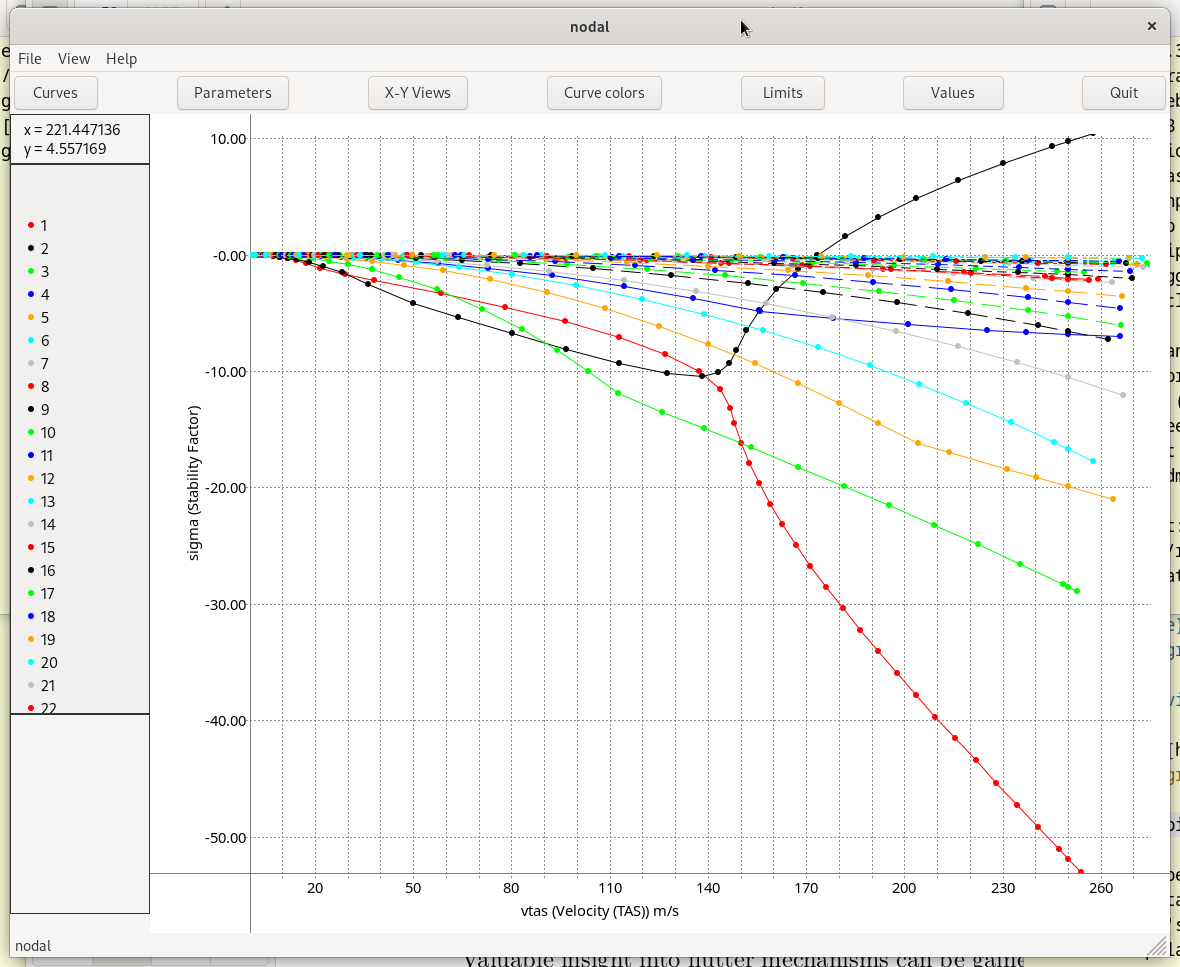
\includegraphics[height=8cm,width=10cm]{viz.png}
	\centering
	\caption{Typical flutter plot using \Cmd{viz}}\label{fig:viz}
\end{figure}
\Cmd{viz} may be run either from the command line or in a \Flaps script;
options are detailed in \Sectref{ref:viz} and
examples of it's usage are in the demo files (\Chapref{chap:examples}).
Various manipulations can be made to a \Cmd{viz} plot with the buttons on top:
\begin{description}
	\item[Curves] allows you to include or exclude curves using wildcards
		\Sectref{app:wildcards}
		and select from a list of all curves; the resulting list will be a
		combination of includes, excludes, and selections.
	\item[Parameters] choose x and y parameters either from a list of all
		parameters or by typing them in.
	\item[X-Y Views] choose an x-y combination from a list of all the x-y parameter
		combinations that have been previously shown.
	\item[Curve colors] choose a scheme for coloring the curves:
		\begin{itemize}
			\item color curves sequentially: first, second, ...
			\item color by plotfile or aid
			\item color by extension, e.g. 1.a, 1.b, ...
			\item color by y parameter name
		\end{itemize}
	\item[Limits] set new plot limits for x and y
	\item[Values/Legend] toggle the left panel between curve legend and parameter values
		at the point chosen with a left mouse click
\end{description}
\begin{figure}[ht] 	% complains if h
		\includegraphics[height=8cm,width=15cm]{viz-manip.eps}
	\centering
	\caption{Manipulating a \Cmd{viz} plot}\label{fig:viz-manip}
\end{figure}

% This same data could be displayed in 3D (projected onto the page) by including
% a $z$ parameter in the \Cmd{vz} command:
% \begin{lstlisting}
% vz -x vtas -y[-15:15] sigma -z freq vso
% \end{lstlisting}
% shown in \Figref{fig:vso3d}.

\section{Animations}\label{sect:animation}
\index{animated modes!visualizing}
\index{visualizing!animations}
Valuable insight into flutter mechanisms can be gained by seeing
even crude animations of a structure fluttering.
Provided the necessary data is available (\Sectref{sect:amdata}) animations
of the structure oscillating at chosen parameter values can be shown.
In \Flaps there are three ways to visualize animations of the structure:
\begin{itemize}
	\item Within a \Flaps job if the \Cmd{viz} (\Sectref{ref:viz})
	   command follows the \Cmd{flut} command to create a 2D plot of flutter
		results, a right-click on a curve will open a window with the structure
		oscillating as it would at that point on the curve.
		\Figref{fig:viz-amviz} shows the result of a right-click.
	\item On the command line the \Cmd{viz} command can be run
		with a plot file from a previous \Flaps run, and right-clicks
		on the curves start the animation as before.
	\item The \Flaps animation program, \Cmd{amviz}, can be run
		on the command line with a Universal file (\Sectref{sect:universal-file}
		to visualize the transformation in the file - usually a set of free-vibration,
		BMA (\Sectref{sect:bma}) or CMS (\Sectref{sect:cms}) modes.
\end{itemize}
\begin{figure}[ht] 	% complains if h
		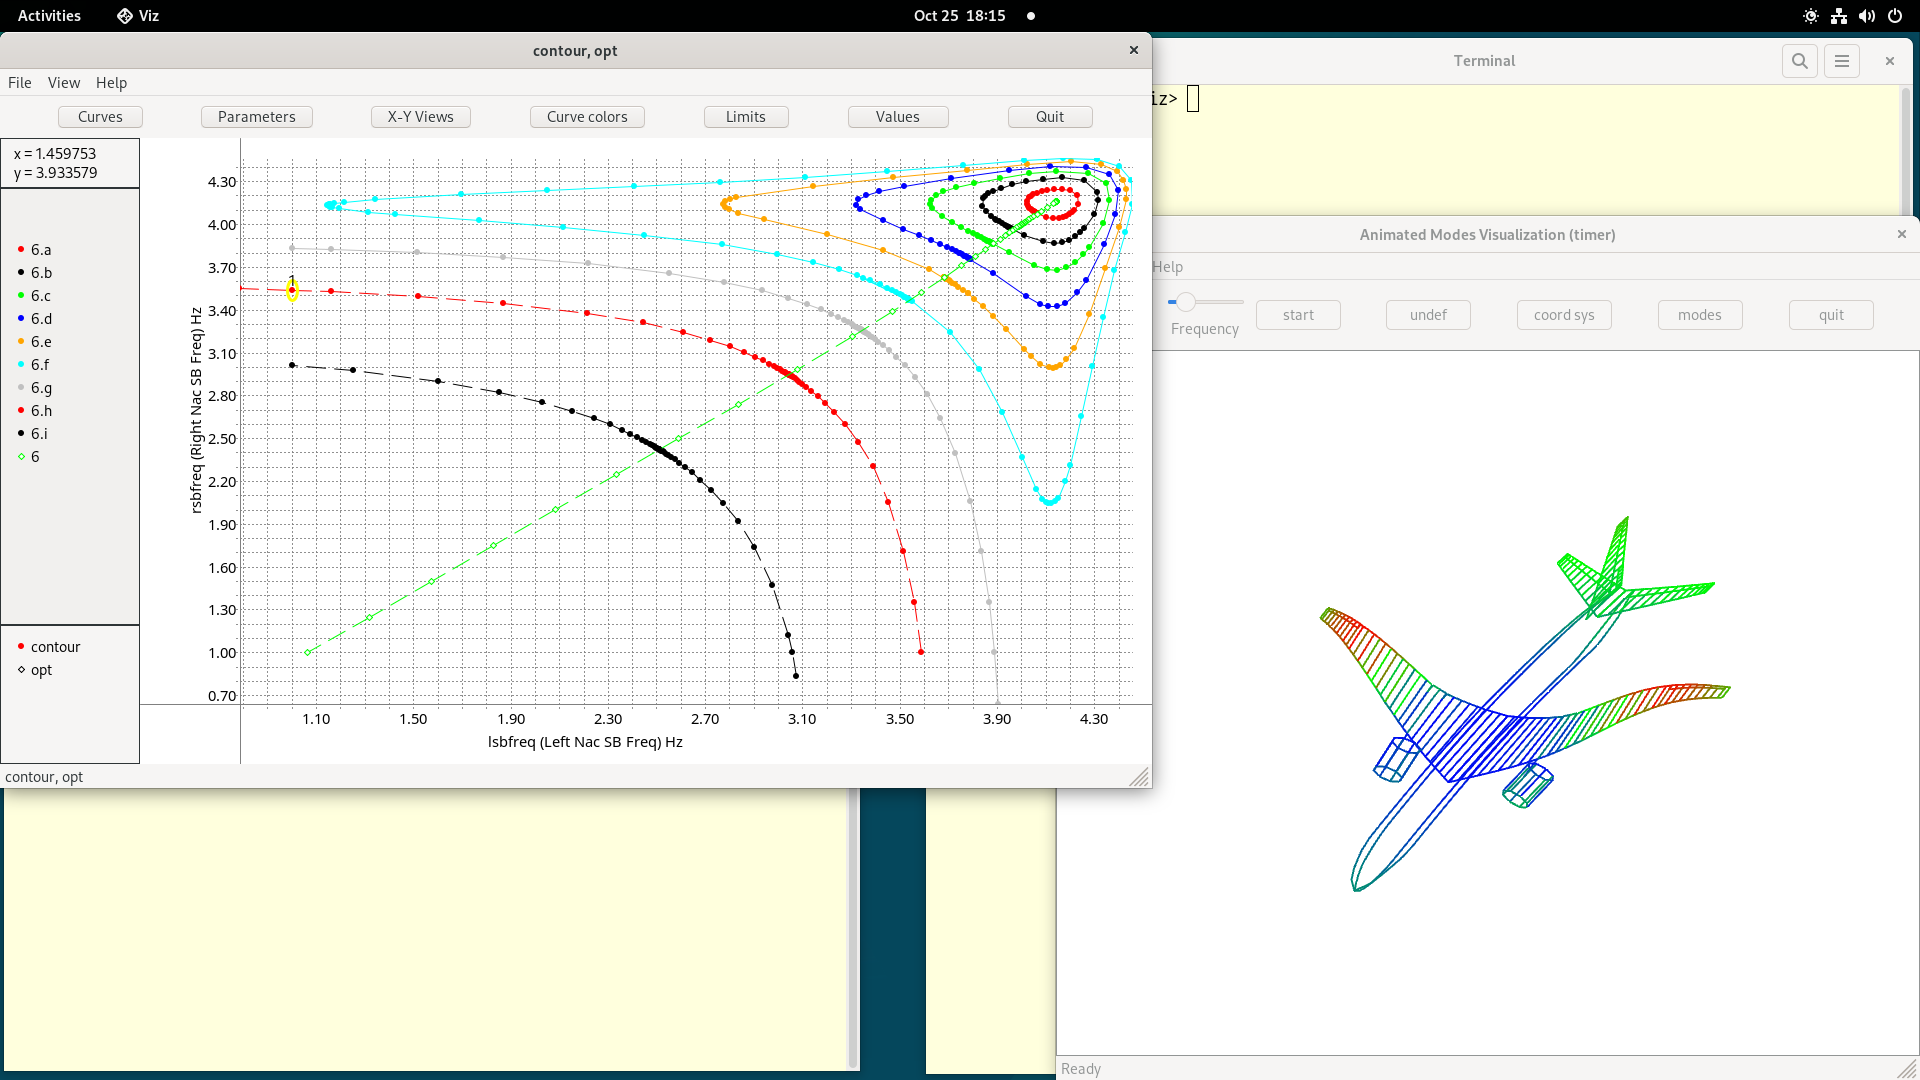
\includegraphics[height=7.2cm,width=13cm]{viz-amviz.png}
	\centering
	\caption{Animated mode from a right-click on a \Cmd{viz} plot}\label{fig:viz-amviz}
\end{figure}
Additional right-clicks can show how an aeroelastic mode changes with the parameters.
It is important to note that although the animation oscillates at
constant amplitude, the actual amplitude may be growing or decaying
depending on the value of $\sigma$ at the chosen point.
Also, the frequency of oscillation will not be correct, since it
is usually not possible to animate at the correct frequency.

Video files (mp4 format) can be created for later viewing with a
program like \Cmd{vlc}.

\subsection{Data requirements}\label{sect:amdata}\index{amviz!data requirements}
In order to understand the data requirements for mode visualization
it helps to understand the process used to produce the animation.
Usually the physical motion of the structure is obtained by \Eqn{eqn:motion}:
\begin{eqnarray} % eqn:motion
% \label{eqn:motion}
\Vector{\chi}(t) & = & \Re \left(\Matrix{\Phi}\hat{\Vector{q}}e^{st}\right) \nonumber \\
              & = & \Re \left[\Matrix{\Phi}\hat{\Vector{q}} e^{\sigma t}
				  			\left(\cos \omega t + i \sin \omega t \right) \right] \nonumber
\end{eqnarray}
where $\Phi$ might be free-vibration modes or dynamic substructuring modes
such as BMA or CMS modes \Sectref{sect:ss-intro}.
\index{=Phi@$\Matrix{\Phi}$!animated modes}
Although these modes would ordinarily change with changes in model parameters,
the usual practice is to keep $\Phi$ fixed, simplifying the solution process
with an acceptable approximation.

$\Phi$ can be thought of as a transformation from the generalized-coordinates
($\hat{\Vector{q}}$) to the displacement of the structure at any given
moment. In addition to $\Phi$, three more items are necessary for animation:
\begin{itemize}
	\item (x,y,z) coordinates of each node
	\item a node number for each node
	\item sets of node numbers defining lines connecting nodes to give
		at least a rough outline of the structure
\end{itemize}

Often the grid used for unsteady aerodynamics can be used, provided
the transformation from generalized-coordinates to the grid is available;
this transformation is part of the unsteady aerodynamics calculation,
but may not be accessible by the user. Besides giving an easy picture
of the motion, using the aero grid gives a check on it's validity.
Some of the example problems (\Chapref{chap:examples})
use the aero grid from the \Cmd{fem} command.

Currently the only external data format recognized is the Universal-file
\cite{UniversalFile}, an ASCII file; \Sectref{sect:universal-file} gives
formats of the relevant sections of a Universal-file.

To use a Universal-file in \Flaps it can be imported
\begin{enumerate}
	\item with the \Cmd{import} command (\Sectref{ref:import}), giving
		the data a \Code{vzid}, which then is used with the \Code{vzid}
		option in \Cmd{flut} to include the \Cmd{amviz} data in plotfiles,
	\item by including the \Code{uf} option in the \Cmd{viz} command
\end{enumerate}
The advantage to the first method is the \Cmd{amviz} data is also included in
plotfiles produced by subsequent \Cmd{flut} commands which use the \Code{source} option.
% Currently the only way to create this data is to \Cmd{import}
% (\Sectref{ref:import}) a file in Universal-file format
% (\Sectref{sect:universal-file}).\index{universal-file}
% There are a few Universal-files in the example problems,
% with \Code{.uf} extensions. They are ASCII files so they can be
% studied with your favorite editor.

\section{Matrix parameterizations}\label{sect:matrix-pz}
Elements of a matrix that is a function of one or more parameters
can be plotted by including the \Code{plot} option in \Cmd{pz} \Sectref{ref:pz}.
Example problem \Code{dlm.fp} \Sectref{ex:dlm.fp} plots elements of the
unsteady aero matrix interpolated with respect to reduced frequency.
and controls.fp demonstrates plotting elements of the \Code{T-matrix}.


% =================================================================
% Chapter Flaps Commands
% =================================================================
\newpage
\chapter{Flaps Commands}\label{chap:commands}

\section{Input file}\label{sect:input-file}
The \Flaps input file consists of one or more \Flaps commands followed by a
line containing only the word \Cmd{end}. Following this set of commands are
optional named sections \index{named section}\index{sections!named}
containing custom functions,
\index{function!custom} \Octlab scripts,\index{matlab@\Octlab!scripts}
or describing-function descriptions. These sections are named, with the syntax
\begin{lstlisting}
name {{
  ...
}}
\end{lstlisting}
and written as files on a temporary directory with the section name.
There are a few restrictions on the name given a section:
\begin{itemize}
\item a section of custom functions must have the name of the entry point
	\Sectref{ref:user-fcn},
\item the name of a section of \Octlab script must end in .m
	\Sectref{ref:octlab},
\item the name of user-defined describing functions is used to identify the
       resulting interpolation coefficients in the \Cmd{dfval} command
		 \Sectref{sect:computing-df}.
\end{itemize}

\subsection{Syntax}\label{sect:syntax}
One of the design goals for \Flaps has been to allow the user
to write input files that are concise, easy to understand, and pleasing to look at.
Rather than requiring strict formatting, \Flaps allows a great
deal of flexibility in how input files are written, allowing
the user to write in his or her favorite style.
It is important to realize that writing \Flaps input files is
``computer programming'' and style does matter, for your
own sake and for the sake of others who may have to read your
computer programs later.
\par
In general, the syntax of a \Flaps command has the form
\par
\hspace{0.5in} \Cmd{command} \{ \Subst{specs\/} \} 
\par
where \Cmd{command} is one of the commands listed in this section.
% \Subst{:aid} is an optional string specifying
% \begin{description}
% \item[analysis identifier] for \Cmd{flut} or \Cmd{vz},\index{analysis identifier}
% \item[matrix name] for \Cmd{display} or the output from \Cmd{pz}
% \end{description}

All \Flaps commands are case-sensitive: there is no \Cmd{Flut},
only \Cmd{flut}.
\index{case sensitivity!commands}
\par
\Subst{specs} are a set of comma-separated specs of the form
\par
\hspace{0.5in} \Spec{keyword} = \Subst{value}
\par
Features of the spec syntax include:
\begin{itemize}
\item \Spec{keyword}s are case-sensitive: \Code{Mass=gm1}
is different from \Code{mass=gm1}.
\index{case sensitivity!spec}
        
\item
\par
if a \Spec{keyword} contains a comma it must be enclosed
in (single or double) quotes to prevent the comma from being
taken as a spec-separator. The same is true of \Spec{value}s.
        
\item 
\par
Some specs do not take a \Spec{value}
        
\item 
\par
Whitespace (space, tab, or newline) characters are ignored except when
enclosed in (double or single) quotes
        
\item 
\par
the comma separating specs may be left off if a
spec is the last one on a line.
        
\item 
\par
in many cases the {\sffamily value} (and sometimes even the {\sffamily keyword})
may be a list with one of the following forms:
\index{list!spec}
                
\begin{description}
\item[\Subst{(i,j,..k)\/}] Explicit list
\item[\Subst{(i:j)\/}] Implicit list: \Subst{(i,i+1,...j)}
\item[\Subst{(i:k:j)\/}] Implicit list with a stride: \Subst{(i,i+k,i+2k,...j)}
\end{description}\label{sect:implicit-list}
Note that an implicit list is the format used in \Octlab, with one exception -
here the lower and upper bounds can be letters, possibly embedded in a string,
for example
\begin{lstlisting}
  (massa3 : 2 : masse3) = (massa3, massc3, masse3)
\end{lstlisting}
\index{implicit list}
\index{list!implicit}
        
\end{itemize}

The {\sffamily value} of a spec may have one of the following datatypes:
\index{spec values}

\begin{description}
\item[{\ttfamily\itshape string}]
\index{string@{\ttfamily\itshape string} (spec value)}A character string of arbitrary length. If the string contains
commas it must be enclosed in single or double quotes so that
the commas are not taken as spec-separators.
\index{quotes!and specs}
As with the Unix shell, environment variables are interpreted
within double quotes, but not within single quotes (see Examples below).
\index{quotes!and environment variables}
\index{environment variable}
      
\item[{\ttfamily\itshape {\ttfamily\itshape integer}\/}]
\index{integer@{\ttfamily\itshape integer} (spec value)}An integer
      
\item[{\ttfamily\itshape {\ttfamily\itshape float}\/}]
\index{float@{\ttfamily\itshape float} (spec value)}A floating-point number, e.g. .7e+1, 7, 7.0 represent the same number
      
\end{description}

\par
Each of these data types may be used in a list if the spec allows;
for example, here are pairs of equivalent specs:
\begin{itemize}
\item \Subst{intlist}
\begin{lstlisting}
   rows = (77:3:89)
   rows = (77, 80, 83, 86, 89)
\end{lstlisting}

\item \Subst{floatlist}
\begin{lstlisting}
   freq = (1.0:0.5:2.5)
   freq = (1.0, 1.5, 2.0, 2.5)
\end{lstlisting}

\item \Subst{stringlist}
\begin{lstlisting}
   plot = (freq, x1:2:x10)
   plot = (freq, x1, x3, x5, x7, x9)
\end{lstlisting}
\end{itemize}

\subsubsection{Regular expressions} \label{sect:regex}
Regular expressions can be used in several places in \Flaps;
here are a few of the most commonly used expressions.
This is a small subset of the capabilities of regular expressions.
Regular expressions are widely used in computer programming and
there are many slightly different implementations, for example
the languages Perl and Python, and the Unix tools \Cmd{sed},
\Cmd{grep}, \Cmd{egrep}, and \Cmd{awk}. The most comprehensive version of
regular expressions is the ECMAScript grammar \cite{ECMAScript},
and that is what is used in \Flaps (and the \Cpp standard library).
\Tableref{table:regex} lists some of the more commonly used expressions.
% \begin{center}
% \begin{small}
\begin{table}[ht]  % table:regex
\begin{tabular}{|c|c|} \hline
{\bf Expression} & {\bf Meaning}  \\ \hline
.    & any character \\ \hline
[...] & one of the characters ... (may contain ranges) \\ \hline
[\^\ \!\!...] & none of the characters ... (may contain ranges) \\ \hline
*    & the previous character or group any number of times \\ \hline
?    & the previous character or group 0 or 1 times \\ \hline
+    & the previous character or group at least 1 time \\ \hline
\{\Subst{n}\}  & the previous character or group \Subst{n} times \\ \hline
\{\Subst{n},\}  & the previous character or group at least \Subst{n} times \\ \hline
\{\Subst{n,m}\}  & the previous character or group \Subst{n} to \Subst{m} times \\ \hline
a$|$b    & either pattern a or b \\ \hline
\end{tabular}
\caption{Regular Expressions} \label{table:regex}
\end{table}
% \end{small}
% \end{center}
\index{regular expressions}

Two regular expressions which are used in this chapter to
show alternative specs are, for example
\begin{lstlisting}
   i(nput)? = file
\end{lstlisting}
which means either
\begin{lstlisting}
   i = file
\end{lstlisting}
or
\begin{lstlisting}
   input = file
\end{lstlisting}
are recognized. The other is, for example
\begin{lstlisting}
   id|aid = string
\end{lstlisting}
which means that either \Code{id} or \Code{aid} are recognized.
Note this particular example could also be written
\begin{lstlisting}
   (a)?id = string
\end{lstlisting}

Regular expressions can also be used to simplify command in
a \Flaps program;
for example, aeroelastic modes in \Cmd{flut} are named according to
several factors (\Sectref{ref:flut}) so to limit the number of modes
plotted in \Cmd{viz} the \Spec{c} spec could be used with a
regular-expression:
\begin{lstlisting}
   viz { ..., c=2.[234].[bc],...}
\end{lstlisting}
which would plot curve\_2.2.b, curve\_2.3.b, curve\_2.4.b, curve\_2.2.c, etc.


\subsubsection{Keyword and value options: Spec-Options}
In some cases the \Subst{keyword} or \Subst{value} may be followed by
options enclosed in curly braces. That is, specs may themselves
sometimes have options.
\index{spec-options}
For example
\begin{lstlisting}
   flut{..., start{freq[0:10], ...}
   pz { ..., i=gaf1{rf=0.01}, ...}
\end{lstlisting}

Sometimes these options are
one or more parameter definitions (\Sectref{sect:parformat}),
which may be as simple as setting a parameter value. For example
\begin{lstlisting}
   pz { ..., o=Cont{gain = 1}, ...}
\end{lstlisting}

or with a more complete description of the parameter \Code{phase}:
\begin{lstlisting}
pz {o=Cont{phase(Control-Law Phase)[-90:90]<57.3 deg/rad> = 0}
   ...
}
\end{lstlisting}

\subsubsection{Examples}
Here are a few examples of specs; more can be found in the
example problems (\Chapref{chap:examples}).
\par
Note the use of quotes to protect the commas in the equation:
\begin{lstlisting}
pz { i=stif, o=Stif, [2,2]="Mass[2,2]*(freq2^2)" }
\end{lstlisting}
\par
Options following matrix names:
\begin{lstlisting}
pz {i=gm1{cg(Center of Gravity)=-4,
    gm2{cg=8}, gm3{cg=16}, gm4{cg=24} }
\end{lstlisting}
\par
Lists of values:
\begin{lstlisting}
flut { id=vso, indep=(freq,vtas,sigma),
      fuel=(0,10,20), start{modes=(1:2:10)} }
\end{lstlisting}
\par
Environment variables are expanded when used in specs; for example
\begin{lstlisting}
settings{env="mat=3"}
flut { ...,  mass=mass$mat, stif=stif$mat, ... }
\end{lstlisting}

\subsubsection{Printed Output}
Printed output presents a dilemma in most structural-dynamics
programs: too much printout makes it difficult to find
the important information; too little printout risks
missing the important points. Warning messages are
often missed because of too much printout.
\par
Two techniques used in \Flaps to reduce the amount of
printout without sacrificing important details are graphic
display of matrices, and a one-line summary of generalized-coordinates
and other vectors.

\subsubsection{Matrix Display}\label{ref:matrix-display}
Matrices are notoriously difficult to present in printed
output. The approach taken in \Flaps is to present all
but the smallest matrices graphically. The \Cmd{display}
command (\Sectref{ref:display})
will display a matrix in a separate window with colors indicating
the size of individual elements. Other \Flaps programs write
matrices to files with .mm extensions (\cite{matrixmarket})
which can be displayed by the \Cmd{matview}
specs to the \Cmd{flaps} command (\Sectref{ref:flaps}).
Figure \ref{fig:matview} is an example of a matrix
displayed in \Cmd{matview}\footnote{\Cmd{matview} was written by Jim Kohl (csm.ornl.gov/$\tilde{\ }$kohl/MatView)}.

\subsubsection{Generalized-Coordinate Summary}\label{ref:gcsummary}
\index{g.c.!summary}
\index{energy!summary}At various places in the printed output generalized-coordinates
(or other vectors such as energy) are summarized in a single line by showing which
element has the largest magnitude, followed by the second largest,
and so on. Next to each element number is a decimal fraction of
the largest component in parentheses.
A typical summary looks like this:
\begin{lstlisting}
28 20(0.39) 19(0.32) 24(0.25) 29(0.24) 41(0.16) 68(0.16)
\end{lstlisting}
which means that generalized coordinate 28 has the largest (absolute) value,
and that value is 1.0. The next largest is 20 which has a
magnitude of 0.39, followed by 19 with a magnitude of 0.32, and so on.
Occasionally you may see a summary like
\begin{lstlisting}
[0.8233]28 20(0.39) 19(0.32) 24(0.25) 29(0.24) 41(0.16) 68(0.16)
\end{lstlisting}

The extra number in square brackets [0.82383] means that the largest
value in the vector is not 1.0 but 0.82383. Note that the numbers
in parentheses have not changed; this is because these numbers are
relative to the
largest, so for example the magnitude of generalized coordinate 20
is $ 0.82383*0.39 = 0.32129 $.

\subsubsection{Number formats \label{sect:numformat}}
Floating point numbers in the control program have a very
flexible format; the following numbers are equivalent:
\begin{lstlisting}
     314
     314.0
     0.0314e+4
     31400.00D-2
     .314E+3
\end{lstlisting}
\par
A complex number u + iv may be represented as either
(u + iv) or (u + vi).
\index{complex number}
For example, the following are valid complex numbers:
\par
\begin{lstlisting}
     (3.14+i6.28)
     (0.0314e+2 + i.628d+1)
     (314D-2 + 0.628e+1i)
\end{lstlisting}

% catalog command --------------------------------------------------------
\Manpg{catalog}
Prints a catalog of \Flaps matrices matching specified
conditions.
\par
By default, \Cmd{catalog} prints a catalog
of all \Flaps matrices;
the list may be limited by specifying a list of matrix names,
or regular-expressions (see \Sectref{sect:regex}).

This command can also be used on the command line to catalog
a plotfile or savefile (\Sectref{sect:utility}).

\paragraph{Output} consists of a list of the matrices matching the
matrix names specified, printed on the standard output file.

\paragraph{Examples}
To catalog all matrices:
\begin{lstlisting}
catalog {}
\end{lstlisting}
To catalog all results from \Cmd{flut}:
\begin{lstlisting}
catalog { "curve,.*" }
\end{lstlisting}
note the name is in quotes to protect the comma.

% display command --------------------------------------------------------
\Manpg{display}

Prints \Flaps matrices to stdout, to a specified
output file, or displays the matrix in an interactive graphical window.

\begin{Optlist}{Specs}{}

\Opt{deriv}{= \Stringlist}{a list of parameter names; the derivative with
respect to each parameter will be output. The special name ``\Spec{0}''
(zero) means the matrix values.}{only the matrix values will be output}

\Opt{o}{= \String}{the name of a file to receive the output}{only an
interactive graphical image of the matrix will be output}

\Opt{name1\{\Spec{opts}\}, name2\{\Spec{opts}\}, ... }{}
{A list of one or more matrix names to be printed.
The matrix name may be followed by parameter values (in curly braces) at
which the matrix is to be evaluated if it has been parameterized (see Examples).}
{none}

\end{Optlist}

\subsubsection{Output}
The rules for where and how a matrix is displayed are arcane; they depend on
if the matrix is numeric (real or complex) or some other data array
(nodes, freedoms, etc), the size of the matrix, and the name of the output file.

\paragraph{Numeric Arrays}
Real and complex matrices are printed on the output file
(the file specified with the \Spec{o} spec if included,
the stdout file otherwise). The format it is printed with depends
on the number of columns in the matrix, the value of the
pagewidth (\Sectref{ref:settings}), and the name of
the output file if included.
\par
If the output file name does not end in \Spec{.mm}
the matrix is printed in human-readable form provided an entire
row will fit within the current pagewidth. The default value
of pagewidth is 130 characters, so for example a real (100,5)
array would get printed in human-readable form but a (100,20)
would be printed in Matrix Market \cite{matrixmarket}
format for viewing in \Cmd{matview}.
If the pagewidth were increased to say, 500 it would be printed
in human-readable format.
\par
If an output file name is specified which ends in \Code{.mm}
the matrix will be printed to the file in Matrix Market \cite{matrixmarket}
\index{matrix!market}
format regardless of its size.

\paragraph{Graphical Display}
By default the matrix is displayed graphically
(see figure \ref{fig:matview}), and
the matrix will be written in Matrix Market format (with a \Code{.mm} extension).
It can be visualized from the command line using the \Cmd{matview}
command \Sectref{sect:utility}.
        
Clicking on an element of the matrix with the left mouse button
displays the value of the element.
Middle-clicking and dragging the mouse selects a region
to zoom-in on, and right-clicking restores the unzoomed view.
        
Matrix elements are colored to indicate values according
to the color map above the matrix. A slider above the
color map distorts the color map; this is often necessary
to make all the non-zero elements visible.
        
\subsubsection{Examples}
The following \Flaps command from demo problem contour.fp
displays the original generalized stiffness matrix and the mass
matrix at \Code{cg=-4}, followed by the stiffness matrix evaluated at
\Code{cg=8} and \Code{freq2=2}, with the values and derivatives with
respect to \Code{cg} and \Code{freq2} displayed in \Code{matview}:
\begin{lstlisting}
display { stif, gm1 }
display { Stif{cg=8, freq2=2, deriv=(0,cg,freq2)} }
\end{lstlisting}

\begin{figure}[ht]
		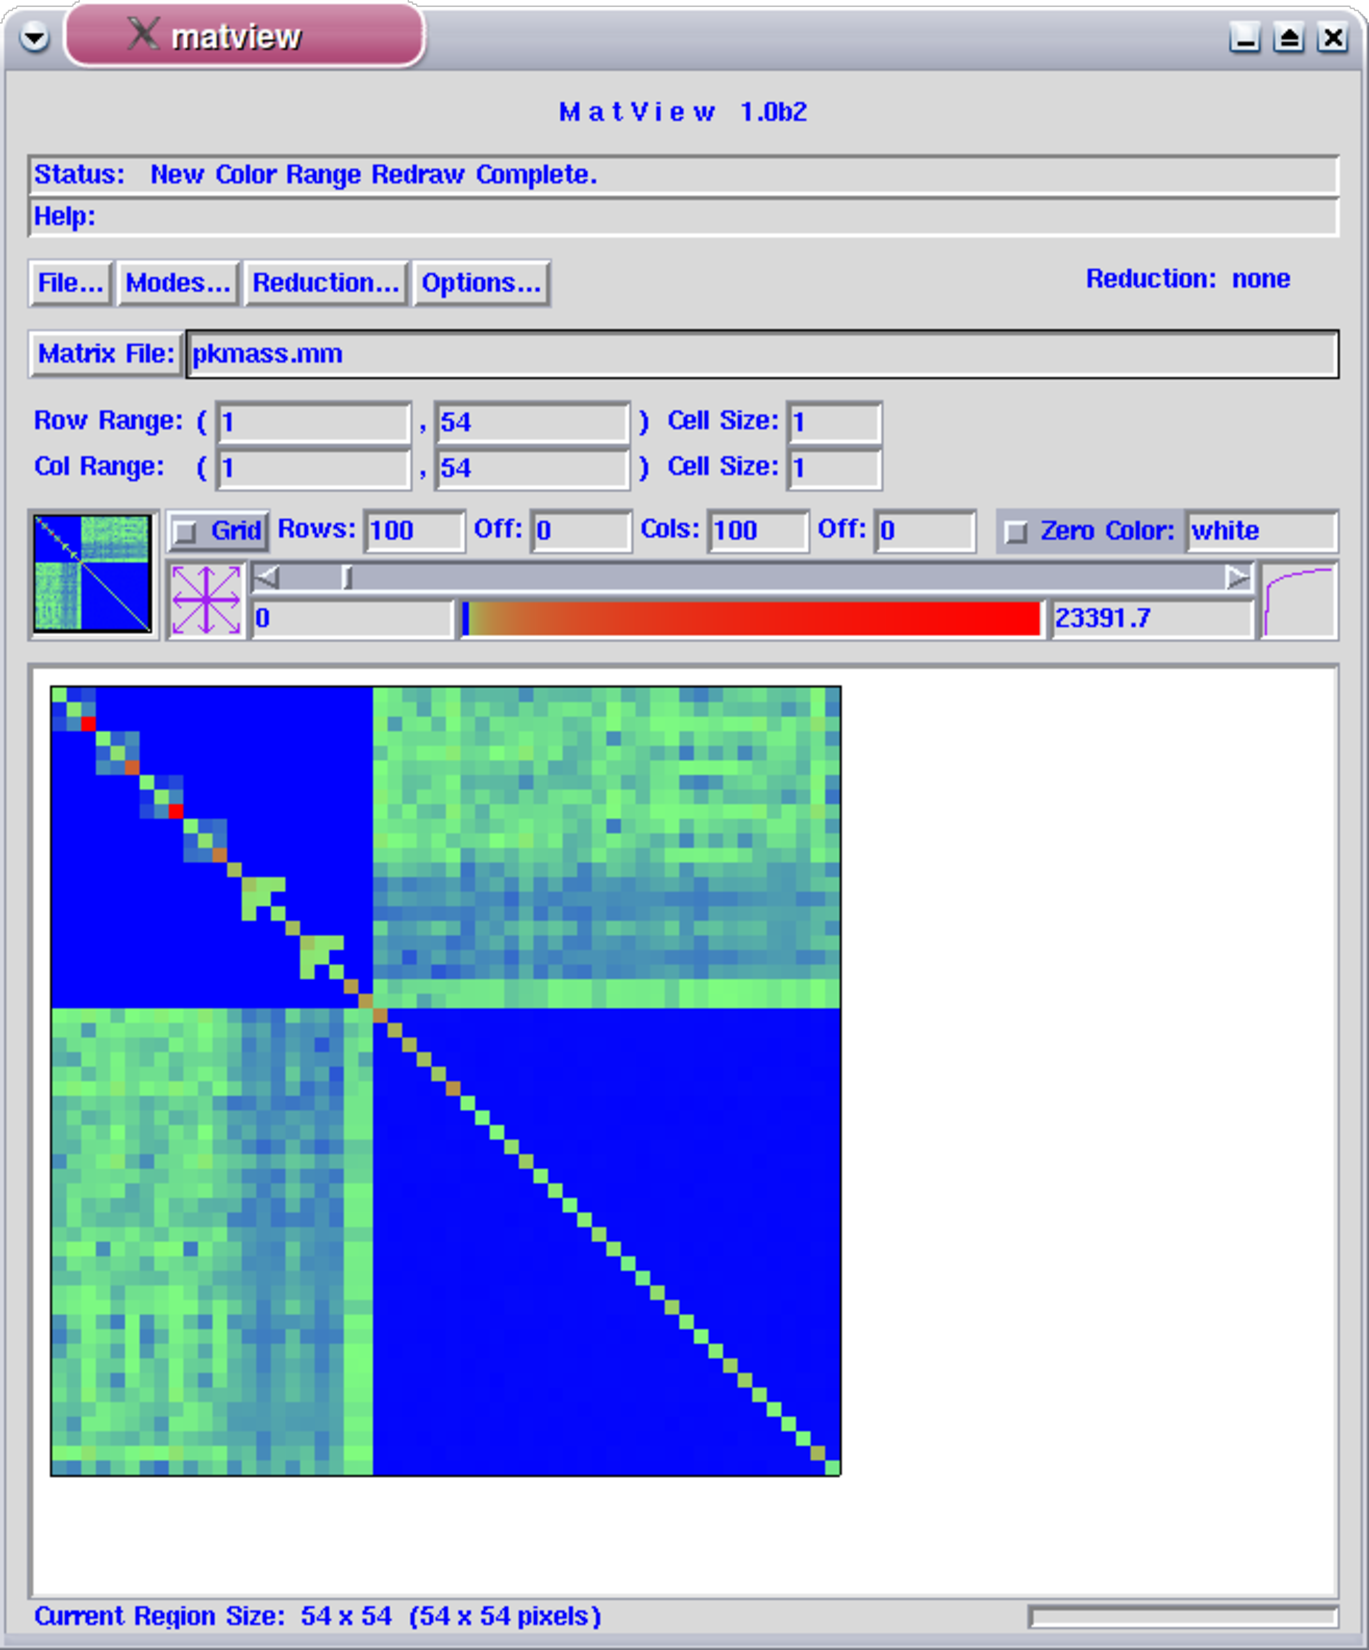
\includegraphics[height=3in,width=3.25in]{matview.pdf}
	\centering
	\caption{Matrix image in \Code{matview}}\label{fig:matview}
\end{figure}

% export command --------------------------------------------------------
\Manpg{export}
Creates a file of \Flaps matrices in one of several formats.

\begin{Optlist}{}{The only specs are the output file name and a list of
matrices. The extension determines the file format, and the matrix list may
include regular-expressions (\Sectref{sect:regex})}

\Opt{o}{= \String}{output file with an extension that determines the format}{fatal error}

\begin{description}
\item[\Code{.mat}] \Octlab format; in \Matlab\index{matlab@\Matlab}
or Octave\index{octave} the \Cmd{load} command will read the file.
\item[\Code{.op4}] \Nastran Output4 format; an ASCII (text) format.
\item[\Code{.mm}] Matrix Market format;
   An ASCII format widely used in the numerical analysis community
   for distributing test matrices. Used for displaying
   large matrices in \Flaps and viewing with \Cmd{matview}
   (\Sectref{ref:matrix-display}) \cite{matrixmarket}.\index{matrix!market}
\item[.fig] an ASCII format used by the open-source drawing program \Code{xfig}.
\end{description}

\end{Optlist}

% fem command --------------------------------------------------------
\Manpg{fem}
Allows for building simple beam models with concentrated masses,
gyroscopics, doublet-lattice and rigid propeller unsteady aerodynamics.
Input consists of one or more of the following subcommands

The global coordinate system used for examples is the traditional one
used with aircraft, shown in \Figref{fig:globalcs}\index{coordinate system!global}.
\begin{figure}[ht]
		\includegraphics[height=4.0cm,width=8.5cm]{globalcs.eps}
%		\includegraphics[height=7.5cm,width=8.5cm]{gyro.pdf}
	\centering
	\caption{Global Coordinate system} \label{fig:globalcs}
\end{figure}

\begin{Optlist}{nodes\{options\}}{a list of node numbers and their coordinates
in the global coordinate system }

\Opt{n}{= \Coord}{global coordinates of node number n.}{none}
\end{Optlist}
For example
\begin{lstlisting}
   nodes{ 1=(0,0,0), 3=(0,1.5,0), 100=(1, 1.5, 1) }
\end{lstlisting}

\begin{Optlist}{beam\{options\}}{description of a single beam element between 2
previously defined nodes; repeated to specify all beam elements}

\Opt{n}{= \Intlist}{1 to 6 degrees of freedom for node number n. This option
must be repeated to specify the second node and (possibly) it's dof}
{If dof are not specified the last list of dof are used}

\Opt{x}{= \Coord}{global coordinates of a point on the local x axis;
bending stiffness of the beam in the local x-y plane is determined by EIx.}
{the last specified coordinates}

\Opt{EIx}{= \Float}{coefficient for bending stiffness in the local x-y plane}
{the last specified value}

\Opt{EIz}{= \Float}{coefficient for bending stiffness in the local y-z plane}
{the last specified value}

\Opt{EA}{= \Float}{coefficient for deformations along the local y axis}
{the last specified value}

\Opt{gj}{= \Float}{coefficient for torsional deformations along the local y axis}
{the last specified value}

\end{Optlist}

\begin{Optlist}{mass\{options\}}{a list of all the concentrate masses in the model,
the node they are attached to, their mass and moment of inertia, and the value and
orientation of its offset from the node}

\Opt{mass}{= \Float}{mass in Kg}
{the last specified value}

\Opt{moi}{= $I_x,I_y,I_z$}{moments of inertia about the global x, y, and z axes}
{the last specified value}

\Opt{orient}{= $(x,y,z)$}{the orientation vector: a point on the line between
the node and the concentrated mass} {the last specified value}

\Opt{cg}{= \Floatorstring}{either the distance (in meters) from the node
to the concentrated mass along the orientation vector, or the name of a parameter
with the distance} {the last specified value}

\Opt{nodes}{= \Intlist}{a list of node numbers where concentrated masses
are attached based on the last specified values of the properties} {none}

\end{Optlist}

\begin{Optlist}{gyro\{options\}}{create a gyroscopic matrix}\label{ref:fem-gyro}
\Opt{node}{= \Int}{node number where the propeller is mounted}{error}
\end{Optlist}

\begin{Optlist}{pgaf\{options\}}{unsteady aerodynamics for a
propeller \Sectref{sect:whirl-aero}, specified as a list of properties
followed by a list of node numbers where the propellers attach}

\Opt{radius}{= \String\ or \Float}{the name of a parameter or the value
of the propeller radius} {1.0 m}

\Opt{beta}{= \String\ or \Float}{the name of a parameter or the value of
the angle of attack of the propeller blade relative to the freestream, in the range
34 to 58 degrees} {34 degrees}

\Opt{lbar}{= \String\ or \Float}{the name of a parameter or the value of the distance
from the node to the propellor hub, divided by the radius} {1.0}

\Opt{orient}{= \Coord}{coordinates of a point on the spin axis} {error}

\Opt{node}{= \Intlist}{a list of node numbers where propellers with the
above properties are attached} {error}

\end{Optlist}

\begin{Optlist}{dlm\{options\}}{unsteady aerodynamics for a 2 dimensional
surface using the double-lattice method \cite{albano1969doublet}.
The output matrix is a one-to-three dimensional interpolation depending
on whether \Code{rf}, \Code{mach}, and \Code{rsf} are specified with multiple values}

\Opt{panels}{= (m,n)}{the number of panels in the chordwise and spanwise
directions. \emph{Note that currently the spanwise panels are determined by
the nodes of the beam to make transferring loads from the aero grid to
the beam model easier}} {error}

\Opt{chord}{= \Float}{length of the chord at the root}{error}

\Opt{ac}{= \Floatorstring}{global x coordinate of the aerodynamic center
($3/4$ chord) at the root, or the name of a parameter (for parameter studies)}
{$(0,0,0)$}

\Opt{mach}{= \Floatlist}{Mach number(s) in the range 0 to 1}{0.5}

\Opt{rf}{= \Floatlist}{reduced frequencies ($\omega/V$) where the
matrices are to be computed} { error }

\Opt{rsf}{= \Floatlist}{reduced stability factors ($\sigma/V$) where the
matrices are to be computed} { 0 }

\end{Optlist}

% flaps command --------------------------------------------------------
\Manpg{flaps}
Reads a file consisting of one or more \Flaps commands and executes them.
Commands may be in a file, or from standard input.

\paragraph{Syntax}
\Cmd{flaps} [ \Subst{specs} ] [ \Subst{filename} ]

\par
\Spec{help}
\begin{quote}
\par
displays the \Flaps User's Manual.
\end{quote}

\par
\Spec{catalog \Subst{file}}
\begin{quote}
\par
list the matrices on \Flaps savefile or plotfile \Subst{file}.
\end{quote}

\par
\Spec{clean}
\begin{quote}
\par
remove any \Flaps temporary directories left from
previous runs.
\end{quote}

\par
\Spec{\Subst{filename}}
\begin{quote}
\par
Name of a file containing the \Flaps input file.
See \Sectref{sect:syntax} for
the structure of this file.
\end{quote}

\begin{quote}
Default: if no \Subst{filename}
is given the behavior depends on whether the \Cmd{flaps} command is entered
from the command line or within a script (e.g. a qsub file):
if the \Cmd{flaps} command
is entered from the command line, \Cmd{flaps} enters interactive mode.
If the \Cmd{flaps} command is run from a script, input is from standard input,
for example from a Unix
\Newterm{here document}
\index{here document}
(\Sectref{sect:syntax}) (see example below).
\end{quote}
\par


\paragraph{Input and Output}
Input is either a file containing \Flaps commands or a set
of commands in the standard Unix input stream \Newterm{stdin}.
\index{stdin}
If \Flaps is run interactively by typing \Cmd{flaps} at
the command prompt, stdin is from what you type; if \Flaps is
run from within a script (perhaps in batch mode) stdin is
conveniently taken from a Unix \Newterm{here document}.
A here document begins with the
{\sffamily $<$$<$} operator followed by a string of characters of your choice; for
example
\begin{lstlisting}
flaps <<@
   import{myfile}
@
\end{lstlisting}

Here documents are convenient because the input to \Flaps can
be placed in the script without creating a separate file,
and environment variables are substituted, so a script like
\begin{lstlisting}
export gm=mass3
export code=massfcn
flaps <<@
   pz {i=\$gm, code=\$code}
@
\end{lstlisting}
is equivalent to
\begin{lstlisting}
flaps <<@
   pz {i=mass3, code=massfcn}
@
\end{lstlisting}
\par
Output from \Cmd{flaps} is normally to the standard Unix
output streams \Code{stdout} and \Code{stderr} unless redirected
\index{stdout}
\index{stderr}
or the \Cmd{settings} command is used to redirect stdout and/or
stderr. See any reference on the Unix operating system for more
details, for example \cite{gilly1992unix}, \cite{abrahams1992unix},
\cite{kernighan1984unix}, or \cite{rosenblatt1993learning}.

\paragraph{Examples}
To run \Flaps from within a script, taking the input from the
same script, using a Unix \Cmd{here} document, and writing
the output on a file named \Code{out} and \Code{stderr} to a
file named \Code{err}:
\begin{lstlisting}
flaps <<EOF >out 2>err
    restore{savefile}
       ...
    end
EOF
\end{lstlisting}

% flut -------------------------------------------------------
\Manpg{flut}
Solves the aeroelastic stability (flutter) equation
producing continuous curves of standard and user-defined
parameters.

\paragraph{Summary.}
A wide variety of solutions are possible depending on the
choice of independent parameters.
Solutions are generally classified as either neutral-stability
\index{neutral-stability}
or parameter variation.
\index{parameters!variations}
The type of solution is controlled by the choice
of independent parameters.
\par
Neutral-stability curves have for independents a parameter
which increases dynamic pressure, e.g. vtas, veas, or
dynamic pressure itself; frequency; and a parameter
that relates to growth or decay of oscillations:
\Code{sigma}, or \Code{sdamp}.
\par
Parameter variations start from a point on a neutral-stability
curve and trace a curve varying another parameter.
\par
Section \ref{sect:predef} lists builtin parameters
and explains how to define new parameters; \Sectref{sect:flutter-eqns}
discusses the flutter equation (\Eqn{eqn:flut}).

\paragraph{Specs} are categorized as
\begin{itemize}
\item Identifying the solution
\item Equation definition specs
\item Which aeroelastic modes to track
\item Output
\end{itemize}

\begin{Optlist}{Identifying the solution}{for plotting and subsequent analyses
is with an \Newterm{analysis identifier} (aid). The \Newterm{source} identifier
is used to specify a previous analysis to use as start points by interpolating
values of a parameter which is constant in the current analysis but varied in
the \Code{source} analysis.}
\index{analysis identifier}
\index{identifier!analysis}

\Opt{aid}{= \String}{may be arbitrarily long but should not contain spaces.}{combination of the independent-parameter names, e.g. vtas-sigma-freq}

\Opt{source}{= aid}{analysis id of a previous flutter solution used as start points}{start points will be from an eigensolution and possibly a homotopy}
\end{Optlist}

\begin{Optlist}{Equation definition specs: Parameters}{Exactly three independent
parameters must be specified (unless the \Code{optimize} spec is included)
and enough fixed parameters to allow all remaining parameters to be derived from these.}

\Opt{indep}{= (\Subst{parameter-name}, ...)}{A list of 3 parameter names
defined to be independent in the solution. These may be builtin
\Sectref{sect:predef} or user-defined parameters.}{fatal error}

% \Opt{derived}{= (string, ...)}{A list of parameters defined to be derived
% in the solution. These may be standard or user 
% defined parameters. See {\bf Traps and Pitfalls} for an explanation
% of when this preferences is necessary.}{parameters are automatically derived if not declared fixed or independent}

\Opt{optimize}{= parameter-name}{The name of a parameter to be optimized using
the continuation-optimization technique (\Sectref{sect:cont-opt}).
When this spec is included the number of independent parameters
can be any number greater than or equal to three.}{none}
\index{continuation!optimization}

\Opt{parameter-defn}{}{Parameters are declared
\Code{fixed}
\index{fixed parameters}
\index{parameters!fixed}
by including
at least the parameter name, an equals sign, and one or more
values (multiple values are enclosed in parentheses and separated
by commas). Parameters may also be given equations as detailed
in \Sectref{sect:pareqns} which make them
\index{derived parameter}
\index{parameters!derived}
\Code{derived}.}{none}
\end{Optlist}

% \underline{Traps and Pitfalls}
% In some rare situations it is necessary to declare parameters derived,
% meaning the program is to find suitable equations in terms of the
% other parameters. The \Spec{derived} preferences does this, and is
% necessary only when the \Spec{source} preferences is included, because
% with the \Spec{source} preferences the default state
% (\Sectref{sect:parstate}) for all parameters
% is the state used in the \Spec{source} run; the default state can
% be changed with the \Spec{indep} or \Spec{derived} preferences or
% by specifying a value or values for the parameter (which sets the state
% to \Spec{fixed}).
% An example of when the \Spec{derived} preferences
% is necessary is when a \Cmd{flut} command uses a fixed value
% for a parameter, followed by another \Cmd{flut} command including
% the \Spec{source} preferences but in the second command the parameter
% must not be fixed but derived from the other parameters:
% \index{parameters!derived}
% \index{derived parameter}
% \begin{lstlisting}
% flut { id=vso, mach=0.8, ...}
% flut { id=pv, source=vso, derived=mach, ...}
% \end{lstlisting}
% Without the \Spec{derived} preferences \Code{mach} would have
% a \Code{fixed} value of 0.8 in the second command.

\begin{Optlist}{Equation definition specs: matrices.}{The matrices used
in \Eqn{eqn:flut} are specified with the following specs}
% where {\sffamily string} is the name of an existing \Flaps matrix. Most are optional; the
% exceptions are {\sffamily mass} and {\sffamily stif}.

\Opt{mass}{= matrix-name}{the name of the matrix to be used as the mass matrix $\Matrix{M}$}{fatal error}

\Opt{stif}{= matrix-name}{the name of the matrix to be used as the stiffness matrix $\Matrix{K}$}{fatal error}

\Opt{vdamp}{= matrix-name}{the name of the matrix to be used as the viscous-damping matrix $\Matrix{V}$}{none}

\Opt{gyro}{= matrix-name}{the name of the matrix to be used as the gyroscopic matrix $\Matrix{G}$}{none}

\Opt{gaf}{= matrix-name}{the name of the matrix to be used as the unsteady aerodynamics matrix $\Matrix{A}$}{none}

\Opt{custom}{= matrix-name}{the name of the matrix to be used as the
   custom matrix $\Matrix{T}$}{none}

\Opt{controls}{= matrix-name}{the name of the matrix to be used as the
   custom matrix $\Matrix{T}$}{none}

\end{Optlist}

\begin{Optlist}{Which aeroelastic modes to track: the \Code{start} spec}{
\index{mode!aeroelastic}
provides a few ways of specifying which modes
to track, by specifying points on curves from a previous analysis if
the \Code{source} spec is included, or by specifying how to perform
a free-vibration solution and which modes to take from it if the \Code{source}
spec is not included.  The \Code{start} spec has the form
\begin{center}
\fbox{\Code{start}\{ \Subst{options} \}}
\end{center}
That is, \Code{start} has its own options, which only apply to the process of
finding start points:}

\Opt{parameter-name}{= \Subst{(float, ...)}}{sets a parameter value or values where the
start points are to be found}{none}
\Opt{parameter-name[\Subst{min}:\Subst{max}]}{}{sets limits for a parameter where start points are to be found}{none}
\Opt{mode}{= (\Subst{(string, ...)}}{names of \Code{source} curves or the
ordinal numbers of the free-vibration modes ordered by increasing frequency}{none}
\Opt{ordinal}{= (\Subst{(int, ...)}}{if a \Code{source} curve has more than one
point which qualifies as a start point this option specifies the nth such point or points}{none}
\end{Optlist}
\par
Some examples will clarify these options.
\begin{lstlisting}
flut {aid=vso, indep=(vtas,freq,sigma)
	 start{vtas=10,freq[0:10]}, ...}
\end{lstlisting}
With no \Code{source} spec this \Code{start} spec says to do
a free-vibration eigensolution with a small amount of aerodynamics
added to the stiffness matrix and use only modes between 0 and 10 Hz
as start points. The \Code{start} spec \Code{vtas=10} only determines the
amount of aerodynamics added to the eigensolution; \Code{vtas} is independent
for the curve tracing.
\begin{lstlisting}
flut {aid=pv, source=vso, indep=(vtas,freq,p1)
	 sigma=0, start{vtas[20:300], ordinal=1}, ...}
\end{lstlisting}
This example takes start points from the previous run for a parameter variation.
In this case the \Code{start} spec is not strictly necessary,
only to eliminate \Code{sigma=0} start points at \Code{vtas=0} and to take
only the first \Code{sigma=0} crossing for each mode.
Note that \Code{sigma=0} could also have been included in the \Code{start}
spec but that would be redundant since it was necessary to declare it
constant outside the \Code{start} spec.
\begin{lstlisting}
flut {aid=contour, source=pv, indep=(freq,p1,p2)
     vtas=(50 : 50 : 200), sigma=0, ...}
\end{lstlisting}
This example does not include the \Code{start} spec so all
parameter-variation curves
from the \Code{pv} run will be searched for velocities 50, 100, 150, and 200 knots
to use as start points for 2-parameter (p1,p2) velocity contours.

specifying the region in which to search for start points.
Limits are specified in the usual way (\Sectref{sect:parformat}), for example
\begin{lstlisting}
flut { ..., start{freq[0:10]}, ...}
\end{lstlisting}

Specifying a value for a parameter is the same as specifying
both limits the same; for example
\begin{lstlisting}
    flut { ..., start{veas[10:10]}, ...}
\end{lstlisting}
is equivalent to
\begin{lstlisting}
    flut { ..., start{veas=10}, ...}
\end{lstlisting}
It is important to note that limits and values in the \Spec{start}
spec only affect the start points; they have no influence on the
aeroelastic modes beyond the start points.

\par
\Spec{modes} = \Intlist
\begin{quote}
\par
a list of the aeroelastic modes to be tracked.
The aeroelastic modes are numbered according to increasing natural
vibration frequency.
\end{quote}

\begin{quote}
Default: all modes in the start region are tracked
\end{quote}



\begin{Optlist}{Output}{Output from \Cmd{flut} consists of printed output,
plot files,
and data stored in the \Flaps database.}

% Printed output is controlled by the \Cmd{print} and \Cmd{target} spec.
% The \Cmd{print} spec specifies which parameters
% are printed; the default is to print the active parameters, multiple-valued
% fixed parameters, and a summary of the generalized-coordinates.
% Most of the output is self-explanatory; \Sectref{ref:gcsummary} explains the
% generalized-coordinate summary. Plotted output is written to one or more
% plotfiles which are usable in the \Cmd{vis} command.  Which parameters
% are included is determined by the \Spec{plot} spec (default is all the
% parameters), and the file name is controlled by the \Spec{plotfile} spec.
% The \Spec{target} spec specifies certain criteria which if met prints the
% results at that point.
% XXX Where should this go?
% Output transformations (\Sectref{OUTPUTTRANSFORMATIONS}) are parameters defined
% with equations \index{output transformation!in flut} containing references to
% the generalized-coordinates. For example
% {\scriptsize \ttfamily
% \begin{lstlisting}
%    flut { ... n7tzvel(Node 7 TZ Vel) = s*n7tz*gc, ... }
% \end{lstlisting}
% }
% where {\sffamily n7tz} is the row of the modes matrix corresponding
% to the tz freedom of node 7. The new parameter {\sffamily n7tzvel}
% will be included in the plot file by default.

\Opt{print}{= \Stringlist}{a list of parameter names to be included in the
printed output. Certain keywords in the list have special meanings
unless there is also a parameter by that name:
\begin{description}
\item[\Code{full}]
   print a one-line summary for each solution point on every solution curve;
   the default is to print the first and last points and any targets found.
\item[\Code{matrices}]
   print all the matrices used in the flutter equation.
\end{description}
}{the independents and a summary of the g.c.}

\Opt{target}{ \{ \Spec{options} \}}{specifies one or more parameter values
   where results are to be computed and printed; additional parameters
   with limits may be included to narrow the window where targets are sought.
   For example,
   \begin{center}
   \Spec{target}\{ growth=(0,0.03), vtas[200:300] \}
   \end{center}
	will print solutions between 200 and 300 knots \Code{tas}
	where \Code{growth} is either zero or 0.03.
	Targets found may be processed with a custom function by including
	the \Spec{process} spec, for example
   \begin{center}
   \Spec{target}\{ growth=(0,0.03), process=myproc \}
   \end{center}
	will pass each target found to the user-supplied custom function \Code{myproc}
	as detailed in \Sectref{sect:target-proc}. }{none} \index{targets!processing}

\Opt{plot}{ = \Stringlist}{a list of parameters to be included in the plot file.}
{all builtin and user-defined parameters are included}

\Opt{plotfile}{ = \String}{name of the file to receive the plot data.}
{\Subst{aid}.pf where \Subst{aid} is specified with the \Code{aid} spec.}
\par
\end{Optlist}

\begin{Optlist}{Curve smoothing}{
Occasionally it is necessary or desirable to modify the behavior of the
continuation method used. The \Code{pac} (pseudo-arclength continuation)
spec has a few options for doing this:

\vspace{10pt}
\hspace{-10pt}\Spec{pac} \{ options \} where the options are:}

\Opt{curvaturefac}{ = \Float}{a factor between 1 and 10 which multiplies the computed
curvature to force the stepsize algorithm to take smaller steps}{4}
\Opt{maxstepsize}{ = \Float}{the largest step to take when tracking a mode}{0.2}
\Opt{minstep}{ = \Int}{the minimum number of steps to take when tracking each mode.}{50}
\end{Optlist}

% gyro command --------------------------------------------------------
\Manpg{gyro}
Creates a gyroscopic matrix ($\Matrix{G}$ in \Eqn{eqn:motion}) by
specifying one or more nodes where spinning rigid bodies are
supported, the moment of inertia of each rigid body, and optionally
the spin rate associated with each one.

\begin{Optlist}{Specs}{}
\Opt{o}{ = \String}{name to be given to the output matrix}{gyro}
\Opt{modes}{ = \String}{the name of a matrix to be used to transform
the gyro matrix to generalized coordinates: $\Phi^t \Matrix{G} \Phi$}
\index{=Phi@$\Matrix{\Phi}$!gyro matrix}
\end{Optlist}

\begin{Optlist}{attachment node number}{
The \Code{node} spec may be repeated to include multiple spinning
rigid bodies in the output gyro matrix.
The \Code{node} spec specifies the number of the node, and has the form
	\begin{center}
	\fbox{\Code{node=\Subst{node-number}}\{ \Subst{options} \}}
	\end{center}
where \Subst{options}, which only apply to the
rigid body attached to the specified node, are:}

\Opt{moi}{= \Float{units}}{The moment of inertia of the rigid body in
	$kg\text{-}m^2$ ($N\text{-}m\text{-}s^2$),
  $lb_m\text{-}in^2$, $lb_f\text{-}in\text{-}sec^2$, or
  $slug\text{-}ft^2$.
% The units may be specified by following the \Float\ with the string
% \Code{N}, \Code{lbm}, \Code{lbf}, or \Code{slugs}.
}{fatal error}

\Opt{orient}{= (\Float, \Float, \Float)}{x, y, and z coordinates of a point on the
	spin axis in the direction of the spin vector and relative to the
	node; this point therefore gives the orientation and direction of the spin
	according to the right-hand rule.}{fatal error}

\Opt{spin}{= \Float}{The spin rate in $rpm$ or $rad/s$, specified
   by following the rate with the string \Code{rpm} or \Code{rad}.
	Note that the gyro matrix will be multiplied by the spin rate
	(in $rad/s$) in \Cmd{flut}, so if the spin rate given here is
	not 1, the \Code{spin} spec in \Cmd{flut} should be set to 1.}{1.0 $rad/s$}
\end{Optlist}

\paragraph{Method}
A rigid body undergoing small displacements given by 3 angles at the node,
\begin{equation}
\Vector{\theta} = \left\{ \begin{array}{c}
			\theta_{1} \\
	      \theta_2 \\
			\theta_3
		\end{array} \right\}
\end{equation}
$\theta_1$, $\theta_2$, and $\theta_3$, and spinning at a rate
$\Omega$ about an axis $\Vector{r}$ will produce moments
about the $x$, $y$, and $z$ axes as illustrated in \Figref{fig:gyro}.
The axis
\begin{equation}
\Vector{r} = \left\{ \begin{array}{c}
			r_1 \\
			r_2 \\
			r_3
		\end{array} \right\}, \hspace{10mm}
		||\Vector{r}||_2 = 1.0   \nonumber
\end{equation}
is specified with the \Code{orient} spec, normalized to length 1.0.

\begin{figure}[ht]
		\includegraphics[height=7.5cm,width=8.5cm]{gyro.eps}
%		\includegraphics[height=7.5cm,width=8.5cm]{gyro.pdf}
	\centering
	\caption{Coordinate system for gyro} \label{fig:gyro}
\end{figure}\index{coordinate system!gyro}
The angular momentum vector of the rigid body is $\Vector{h} = I\Omega\Vector{r}$
where $I$ is the moment of inertia. Moments at the node are due to the rate of
change of the angular momentum vector
\begin{equation}
\Vector{m} = \dot{\Vector{h}} = \dot{\Vector{\theta}} \times \Vector{h}
	= - \Vector{h} \times \dot{\Vector{\theta}}
\end{equation}
In matrix notation the cross product is
\begin{equation}
\Vector{m} = -I\Omega\left[ \begin{array}{ccc}
			0     &   -r_3  &  r_2  \\
	      r_3  & 0     &   -r_1   \\
	      -r_2  & r_1     &   0
		\end{array} \right]
		\left\{ \begin{array}{c}
			\dot{\theta_1} \\
			\dot{\theta_2} \\
			\dot{\theta_3}
		\end{array} \right\}
\end{equation}
so the gyro matrix is
\begin{equation}
\Matrix{G} = I\Omega\left[ \begin{array}{ccc}
			0     &    r_3  &  -r_2  \\
	      -r_3  & 0     &   r_1   \\
	       r_2  & -r_1     &   0
		\end{array} \right]
\end{equation}
with units $kg\text{-}m^2/s = N\text{-}m\text{-}s$.
% \begin{equation}
% N\text{-}m\text{-}s or (lb_f\text{-}in\text{-}sec^2)(rad/sec)(rad) = lb_f\text{-}in\text{-}sec/rad^2 \nonumber
% \end{equation}
% or $lb_f\text{-}in\text{-}sec$ if it has been transformed into generalized
% coordinates.

% \begin{eqnarray}
% \frac{slug}{ft^2} &=& \frac{14.593903}{0.3048^2} = 157.087464 \nonumber \\
% \frac{lb_m}{in^2} &=& \frac{0.45359237}{0.0254^2} = 703.0695796
% \end{eqnarray}

% import command --------------------------------------------------------
\Manpg{import}
Reads files in various formats and creates \Flaps matrices from the contents.

\begin{Optlist}{Specs}{}
\Opt{i}{= \String}{The path of the file to be imported}{fatal error}

\Opt{format}{= \String}{The format of the data in the file.
   It is normally not necessary to specify the format - it can be determined
   from the file extension if the default extension is used,
   or by examining the data. Valid formats are:
\begin{description}
\item[\Spec{output4}] \Nastran OUTPUT4-formatted ASCII
file. Default extension: \Code{.op4}.
\item[\Spec{matlab}] \Octlab MAT-file formatted binary file (uncompressed).
Default extension: \Code{.mat}.
\item[\Code{matrix market}]
An ASCII format widely used in the numerical analysis community
for distributing test matrices. Used for printing
large matrices in \Flaps and viewing with matview
(\Sectref{ref:flaps}) \cite{matrixmarket}.
\index{matrix!market}
Default extension: \Code{.mm}.
\item[\Code{universal}]
An ASCII format originally from SDRC, widely used to
transfer data to laboratory test software.
Only formats 15 (nodal), 55 (modes) and 82 (connectivity)
are allowed (format 164 (units) is ignored). The formats are documented
at \cite{UniversalFile} and in \Sectref{sect:universal-file}.
\index{universal-file!importing}
The data in a universal-file is used to create animated aeroelastic
modes with \Cmd{amviz} by right-clicking on a a curve produced by the
\Cmd{viz} command.\index{amviz!input data}\index{animated modes!requirements}
Default extension: \Code{.uf}.
\end{description}
}{determined from the file extension}
\end{Optlist}

% lti command --------------------------------------------------------
\Manpg{lti}
Creates the $\Matrix{T}$ matrix in \Eqn{eqn:flut} representing linear
time invariant controls equations by converting an ABCD state-space representation
to the $\Matrix{T}$ matrix in \Eqn{eqn:flut}. Details of this conversion are
in \Sectref{sect:abcd-conversion}.
\index{LTI control system!\Cmd{lti} command}

The output $\Matrix{T}$ matrix is evaluated by a custom function
which is compiled and made available to all subsequent commands that
use this matrix. The source code for this custom function is on the
working directory and has the name specified with the \Cmd{i} option
followed by \Code{.cpp}.

\begin{Optlist}{Specs}{}
\Opt{i}{= \String}{The path of the file containing data described in \Sectref{sect:ABCD-file}}{fatal error}
\Opt{o}{= \String}{The name to be given to the output $\Matrix{T}$ matrix}{$\Matrix{T}$}
\Opt{psi}{= \String}{The name of the $(n_i,n_e)$ matrix, $\Phi$ in \Eqn{eqn:abcd-uq} }{fatal error}
\Opt{stif}{= \String}{The name of the stiffness matrix, $K$ in \Eqn{eqn:flut} }{fatal error}
\Opt{e}{= \String}{a description of the columns of $K$ comprising $E$ in \Eqn{eqn:lti-f}}{fatal error}
\Opt{igain}{= (\Floatorstring,...)}{a list of $n_i$ parameter names or values of the input gains}
	{(1,1,..)}
\Opt{iphase}{= \Floatorstring}{a list of $n_i$ parameter names or values of the input phases}
	{(0,0,...)}
\Opt{ogain}{= \Floatorstring}{a list of $n_o$ parameter names or values of the output gains}
	{(1,1,...)}
\Opt{ophase}{= \Floatorstring}{a list of $n_o$ parameter names or values of the output phases}
	{(0,0,...)}
\end{Optlist}


% octlab command --------------------------------------------------------
\Manpg{octlab}
Run \Matlab\index{matlab@\Matlab} (or the open-source alternative Octave)
\index{octave} with a script to manipulate \Flaps matrices, or provide any
of it's extensive capabilities. Which is used (\Matlab or Octave) depends
on the current PATH; the first one found will be used.

\begin{Optlist}{}{There are only 2 specs: input to \Octlab, and
the names of matrices to be brought back}

\Opt{i}{= \Stringlist}{name of the section in the \Flaps script or the path of a file containing \Octlab, commands, and a list of matrices to be sent with
the script}{fatal error if a script is not given, all matrices if no names given}
\Opt{o}{= \Stringlist}{names of the matrices to be returned to \Flaps}{all matrices}

\end{Optlist}

% parameter command --------------------------------------------------------
\Manpg{parameters}
Creates new parameters or modifies existing ones based on its string
arguments, descriptions of the parameters, as detailed in \Chapref{chap:parameters}.
An example taken from demo problem reed.fp (\Sectref{ex:whirl}):
\begin{lstlisting}
   parameters{spin(Spin rate (rpm))[0:5000]<radps2rpm> = 1}
\end{lstlisting}
When the name of one of the builtin scalars
(\Sectref{sect:scalars}) like \Code{radps2rpm} are used in
the conversion factor, the resulting parameter definition
is expanded to
\begin{lstlisting}
   spin(Spin rate (rpm))[0:5000]<9.5493 rpm/(rad/s) = 1>
\end{lstlisting}

Multiple parameter definitions should be on separate lines:
\begin{lstlisting}
   parameters{
      spin1(Prop 1 spin rate)[0:2000]<radps2rpm> = 100
      spin2(Prop 2 spin rate)[0:2000]<radps2rpm> = spin1
      beta1(3/4 blade angle)[34:58]<degrees>=34.0
      beta2(3/4 blade angle)[34:58]<degrees>=34.0
      radius(Prop radius)=0.5
      lbar1(l/r)[0.1:2]=0.1
      lbar2(l/r)[0.1:2]=0.1
   }
\end{lstlisting}

% pz command --------------------------------------------------------
\Manpg{pz}

The \Cmd{pz} command is used to create matrices
that are functions of arbitrary parameters.

\subsubsection{Summary}
Several types of parameterizations are available; in roughly increasing
order of generality they are

\begin{description}
\item[matrix element]
   assign an equation to a matrix element
        
\item[interpolation]
   cubic spline interpolation in 1, 2, or 3 variables
	\index{aerodynamics!interpolation}

\item[rational function approximation (RFA)]
   approximate a set of generalized aerodynamic matrices
   as a function of complex reduced frequency (\Sectref{sect:rfa-theory})
	\index{aerodynamics!approximation}
                        
\item[custom evaluation function]
   associates a \Cpp function with a new or existing matrix; the
   matrix is passed to the function where it can be arbitrarily modified.
   This option requires some knowledge of \Cpp.

\item[describing-function creation]
   given a description of a nonlinearity in the time-domain,
   this option creates a describing function which can be used in
   a matrix-element equation or in a custom function. This also
   requires some knowledge of \Cpp.
                
\end{description}

\par
Multiple parameterizations can sometimes be associated with
a matrix. For example, problem \Code{whirl.fp} \Sectref{ex:whirl}
creates an unsteady aerodynamics matrix with the \Cmd{fem} command
consisting of doublet-lattice aerodynamics for the wing and Reed
(\cite{reed1961analytical})
aerodynamics for the propellers; the doublet-lattice aerodynamics
are parameterized by interpolation with respect to reduced-frequency,
followed by a custom-function parameterization for the propellers.
	\index{aerodynamics!interpolation}
% a set of unsteady-aerodynamics matrices could
% be interpolated with respect to reduced-frequency, then passed to a
% custom function where a describing-function might be applied.
Not all combinations make sense; interpolation and RFA cannot
be used on the same matrix. Custom evaluation functions
are the most general type of parameterization, and
can be used with virtually any matrix and any other parameterization.

See \Sectref{sect:syntax} for the general syntax of specs.
\par
Specs are categorized as
\begin{itemize}
\item General specs
\item Matrix element
\item Interpolation
\item Rational function approximation
\item Custom evaluation functions
\item Describing functions
\item Plot specs
\end{itemize}

Input matrices are specified with the \Spec{input} (or just \Spec{i})
spec either as a list enclosed in parentheses, or individually, for example
\begin{lstlisting}
   pz { i=(m1, m2, m3, m4), o=fuel }
\end{lstlisting}
is the same as
\begin{lstlisting}
   pz { i=m1, i=m2, i=m3, i=m4, o=fuel }
\end{lstlisting}

Parameters may be associated with matrices by following the
name with one or more comma-separated parameter names
enclosed in curly braces; for example
\begin{lstlisting}
   pz { i=(gaf0{rf=0, rsf=0, mach=0},
           gaf08{rf=0.08, rsf=-1, mach=0.4}, gaf0015{rf=0.0015}
           gaf10{rf=0.10, rsf=1, mach=0.8})
      }
\end{lstlisting}
will interpolate the matrices with respect to the 3 parameters \Code{rf},
\Code{rsf}, and \Code{mach} which are builtin parameters (\Sectref{sect:predef}).

A new parameter\index{parameters!creating}
may be associated with a matrix by following the
name with a new parameter definition (\Sectref{sect:parformat}).
For example
\begin{lstlisting}
   pz { i = (gm1{fuel(Percent Fuel)[0:100]=0},gm2{fuel=25},
        gm3{fuel=50},gm4{fuel=75},gm5{fuel=100}), o = Mass }
\end{lstlisting}
interpolates 5 mass matrices with respect to a new parameter called \Code{fuel},
creating a new matrix called \Code{Mass}. Continuing with this example,
if the matrix is already a function of the parameter in curly braces
it will be evaluated at the parameter value. So, for example the statement
\begin{lstlisting}
   pz { i = Mass{fuel=0}, i = Mass{fuel=100} o = LMass }
\end{lstlisting}
will create a new matrix \Code{LMass} which is a linear
interpolation between \Code{gm1} and \Code{gm5}.

\begin{Optlist}{General specs}{}

\Opt{i}{= \Stringlist}{The name of the input matrix or a list of names
enclosed in parentheses.}{none}

\Opt{o}{= \String}{The name given to the output matrix.}{Name of the input matrix if there is only one, fatal error otherwise.}

\Opt{datatype}{= \Code{real} or \Code{complex}}{The data type to be given to the output matrix.}{The output matrix usually has the same datatype as the input matrix
unless the parameterization requires casting the matrix to a different
datatype; for example applying a structural damping parameterization
to a (real) stiffness matrix requires the output matrix be complex.}
\end{Optlist}


\begin{Optlist}{Parameterizing Matrix Elements}{Individual elements of the output
matrix may be given equations by specifying the row and column numbers
in square brackets on the left and the equation on the right side of
the equal sign.}\label{opt:matrix-element}
\Opt{[row,col]}{ = \String}{equation which will replace the element in the output matrix (\Sectref{sect:pareqns})}
{none}
\end{Optlist}
\index{parameterization!matrix element}

For example
\begin{lstlisting}
[27,25] = 3.2*lnvb*log10(alt)*sqrt(Mass[27,27])
\end{lstlisting}

sets the (27,25) term of the output matrix to an equation
involving a user-defined parameter (\Spec{lnvb}),
standard parameter \Spec{alt}, and the (27,27) element
of a matrix called \Spec{Mass}.

\begin{Optlist}{Interpolation}{If there is more than one input matrix, the
\Spec{beta} spec is not included, and the matrices are functions of the same
1 to 3 parameters, the matrices are fitted with a
\Newterm{cubic spline}.}
\Opt{i}{ = \Stringlist}{list of input matrices; each name should be followed
by a list of the parameters the matrix is a function of, and their values.
}{interpolation is only triggered if multiple input matrices are specified}
\index{spline}
\index{interpolation}
\end{Optlist}

\begin{Optlist}{Approximation}{Approximation of a set of unsteady aerodynamic
matrices by a rational-function approximation (RFA) (\Sectref{sect:rfa-theory})
is triggered by including the \Spec{beta} spec.
The input matrices must be functions of \Spec{rf}, and possibly
\Spec{rsf} (\Tableref{table:stdpl-eqns}).}
\Opt{beta}{ = \Floatlist}{Values of $\beta$ used in the
rational-function approximation.}{RFA is not used}
\end{Optlist}
\index{approximation}
\index{s-plane approximation}
\index{RFA}

\begin{Optlist}{Custom evaluation functions}{A custom function
parameterization can be used to modify an existing matrix or to
create a new matrix. If an input matrix is not specified a new matrix
will be created and passed to the custom function. If one input
matrix is specified it will be passed to the function; and if multiple
input matrices are specified they will either be interpolated or
approximated with RFA if the \Cmd{beta} spec is included
(unsteady aerodynamics matrices only).  \label{ref:user-fcn}
\Sectref{chap:functions} has guidelines for writing a function.}
\index{custom function!matrix parameterization}
\index{function!custom}
\index{parameterization!custom function}

\Opt{code}{ = \Subst{file}}{Name of a file (or a section in the \Flaps input file)
containing a set of \Cpp functions which modifies the input matrix. One of these,
referred to as the \Newterm{entry point}, must have the same name as the
file or section.}{none}
\par
The dimensions of the output matrix are determined by the
dimensions of the input matrix and optionally extra rows
and columns specified with the \Code{extra} spec,
or if there is no input matrix by the \Code{size} spec.
\par
\Opt{size}{ = \Stringlist}{If no input matrix is specified size of the
output matrix must be specified either with the name of an existing
matrix or row and column dimensions.
%% the list can of one or two strings: the first specifies the row dimension and the
%% second the column dimension. Specifying only one string yields a square matrix.
%% The strings can be either integers or the name of an existing matrix.
%% If a matrix name is specified the corresponding row or column
%% dimension will be taken from the matrix.
}{dimensions of the input matrix}
\par
For example, if \Code{Sensor} is an existing (3,5) matrix
and \Code{Stif} is an existing (5,5) matrix
\begin{lstlisting}
   size = (3,5)
   size = (Sensor,5)
   size = (3, Sensor)
   size = (Sensor, Stif)
\end{lstlisting}
all produce the same size matrix, and
\begin{lstlisting}
   size = (5,5)
   size = 5
   size = Stif
\end{lstlisting}
all produce a (5,5) matrix.

\Opt{extra}{ = \Rhs{int}}{The number of extra degrees of freedom to include
in the output matrix.  Extra rows and columns are appended to the bottom
and right of an existing input matrix.}{no extra dof are included}
\end{Optlist}

The code is compiled in the \Cmd{flaps} command before any processing
takes place. The functions are then made available to all \Flaps commands;
all that takes place here is to include a call to the entry point in the
evaluation of the matrix.

\begin{Optlist}{Plot specs}{It is sometimes useful to plot elements
of parameterized matrices to check the parameterization; this can be done
by including the \Code{plot} spec followed by plot options
enclosed in braces. The \Spec{indep} option specifies the parameter(s)
to be varied and their limits; other parameters may be set
constant by listing them with with a value on the right-hand-side.
The output plotfile is the name of the output matrix with a \Code{.apf}
extension.  The options are:}

\Opt{indep}{ = \Stringlist}{a list of one or two parameters to be varied for plotting}{
all parameters the output matrix is a function of, except parameters declared \Spec{fixed}.}

\Opt{parameter-defn}{}{Parameters are declared \Spec{fixed} by including
    at least the parameter name, an equals sign, and one or more
    values (multiple values are enclosed in parentheses and separated
    by commas). Parameters may also be given equations as detailed
    in \Sectref{sect:pareqns} which make them \Spec{derived}.}{none}

\Opt{diag}{}{plot all the diagonal elements}{none}
                
\Opt{diag}{ = \Intlist}{a list of diagonal elements}{none}
                
\Opt{row}{ = \Intlist}{a list of rows to plot; if the \Spec{col} option is
	 also included, the elements will also be limited to those columns.}{none}

\Opt{col}{ = \Intlist}{a list of columns to plot; if the \Spec{row} option is
	 also included, the elements will also be limited to those rows.}{none}
                
\Opt{[\Subst{i,j}]}{Plot the element in row \Subst{i}, column \Subst{j}.
		 This option may be repeated as many times as necessary.}{none}
\end{Optlist}

\subsubsection{Examples}
The following \Flaps command examples are taken from sample
problem \Cmd{contour.fp}.  The first command creates a interpolation matrix
named 'Mass' that has the parameter 'cg'. Four finite-element mass
matrices were created in \Nastran with centers of gravity varying
from -4 to 24, then reduced to generalized mass matricies with
free-vibration modes at cg=8. The first use of the new parameter gives
it the description ``Center of Gravity'':
\begin{lstlisting}
   pz {i=(gm1{cg(Center of Gravity)=-4.0}, gm2{cg=8.0},
	    gm3{cg=16.0}, gm4{cg=24.0}), o=Mass}
\end{lstlisting}

\par
The next example creates a parameterized stiffness matrix
by giving the $(2,2)$ diagonal an equation based on another
new parameter, \Code{freq2}, defined before \Cmd{pz}
with the command (\Sectref{ref:parameters})
\begin{lstlisting}
parameter{freq2(Second mode freq)[0:10]<radps2Hz> = 2}
\end{lstlisting}
which gives the parameter a description, limits, and a conversion
factor so that plot values are in Hz but internally the values are
in radian/sec. Then the following \Cmd{pz} command creates a new
matrix with an equation for the $(2,2)$ diagonal:
\begin{lstlisting}
   pz { i = stif, o = Stif, [2,2] = "Mass[2,2]*(freq2^2)"}
\end{lstlisting}
The output matricies from these parameterizations are used in
\Cmd{contour.fp} for parameter variations.
\par
Example custom-function \index{function!custom}
parameterizations are in example files
controls.fp, latent.fp, nl2.fp, nl3.fp, and nl4.fp.

% restore command --------------------------------------------------------
\Manpg{restore}
Restore all matrices from a specified file.
\begin{Optlist}{Specs}{}
\Opt{i(nput)?}{ = \Subst{path}}{path of the file to read the matrices}{savefile}
\end{Optlist}
All matrices on the savefile will be restored. Note that because
plotfiles from \Cmd{flut} are savefiles, they may be restored,
for example
\begin{lstlisting}
   restore{ vso.pf }
\end{lstlisting}


% save command --------------------------------------------------------
\Manpg{save}
Save one or more matrices on a specified file.
\begin{Optlist}{Specs}{}
\Opt{o(utput)?}{ = \Subst{path}}{path of the file to receive the matrices}{savefile}
\end{Optlist}
The matrices to be saved may be regular-expressions, for example
\begin{lstlisting}
   save{ .* }
\end{lstlisting}
will save all matrices (the default), and
\begin{lstlisting}
   save{ curve.* }
\end{lstlisting}
will save all curves from \Cmd{flut}.


% settings command --------------------------------------------------------
\Manpg{settings}

Set specs controlling behavior of subsequent commands.

\begin{Optlist}{Specs}{ See \Sectref{sect:syntax} for the general syntax of specs.}

\Opt{units}{ = USCS}{presentation units (\Sectref{sect:units}) will be in the
	United States Customary System of units. This command should be placed
	at the beginning of a \Flaps input file so that the builtin parameters
	will be given USCS presentation units\index{units!presentation}
	prior to any printout or plot-file creation.}{SI units}

\Opt{out}{ = \String}{file name where standard output is to be redirected}{none}

\Opt{err}{ = \String}{file name where standard error is to be redirected}{none}

\Opt{env}{ = \String}{environment variable to be set for subsequent
	commands. The right-hand-side must be a quoted string.
	Double quotes and single
	quotes behave differently in the way that environment variables
	are handled: if the right-hand-side is enclosed
	in double quotes any environment variables in the quotes are
	expanded when the control program starts. Single quotes delay
	the expansion until the \Cmd{settings} command is executed.
	This would make a difference if an environment variable is changed in the
	control program and later referenced; see Examples.}{none}
	\index{environment variable!setting}
	\index{quotes!and environment variables}


\Opt{pagewidth}{ = \Int}{change the maximum width of subsequent printout}{100}

\Opt{timer}{ = \Int}{change the amount of timing information.
Some \Flaps commands write a table of times spent for
various parts of the command to stderr; setting the
level of print to zero means the table will not be written.
Setting the level to 1, 2, or 3 gives more detailed
timing information.}{1}
\end{Optlist}

\subsubsection{Examples}
To write subsequent output to a file named junk on the
home directory, and to discard standard error:
\begin{lstlisting}
settings { out=~/junk, err=/dev/null }
\end{lstlisting}
\index{environment variable}
The file \Code{/dev/null} is the standard Unix trashcan
\index{devnull@/dev/null}
(anything written to this file is discarded).

% As an example of setting environment variables from within
% an \Flaps control program consider
% \begin{lstlisting}
% export Lnv=lnv
% flaps << @
%    settings { env="Lnv=\${Lnv}a" }
%      ...
%    settings { env="Lnv=\${Lnv}c" }
% \end{lstlisting}
% 
% After the first \Cmd{settings} statement environment variable
% Lnv is \Code{lnva}, after the second it is
% \Code{lnvab}, but after the third it is
% \Code{lnvc} due to the use of double quotes instead of single quotes;
% double quotes mean the environment variable is replaced when the
% control program is read by \Flaps whereas an environment variable
% in single quotes does not get replaced until it is used - in this
% case when the \Cmd{settings} statement is executed.
\par
Environment variables can be used to streamline control programs;
for example to create and use an identifier for a job 
\begin{lstlisting}
   settings { env="id=pk85" }
     ...  flut { id = \$id, plotfile = \$id.pf, ... }
     ...
   viz { id = \$id, o = \$id.uf, ... }
\end{lstlisting}


% viz command --------------------------------------------------------
\Manpg{viz}

A system for viewing results from \Cmd{flut}
and optionally viewing animations of aeroelastic modes selected
interactively from points on the 2D plots.
\Cmd{viz} may also be run from the command line, as detailed in
\Sectref{ref:viz-cmdline}.
When \Cmd{viz} is run in a \Flaps script the \Code{aid} option
is used to specify one or more previous executions of \Cmd{flut},
and the \Code{pf} option is used to include data in one or more
plotfiles in binary format (with \Code{.pf} extensions) or
ASCII format (with \Code{.apf} extensions).
\Sectref{sect:apf-file} gives the format of \Code{.apf} files.

\paragraph{Specs}
See \Sectref{sect:syntax} for the general syntax of specs.

\paragraph{Source of the data} to be plotted is specified
using either the \Code{aid} spec, or the \Code{pf} spec,
or both; Either spec can take multiple right-hand-sides.

\begin{description}
\Opt{id|aid}{= (string,...)}{Analysis id(s) from a previous execution of \Cmd{flut}}{none}
\Opt{pf}{= (string,...)}{plotfile(s) (either \Code{.pf} or \Code{.apf} files)
	from a previous execution of \Cmd{flut}}{none}
\end{description}

\paragraph{Parameters} x, y, and optionally z and w are the names listed
in \Tableref{table:stdpl-eqns} or user-defined parameters (\Sectref{sect:newpar}).
% 2D plots may have one or both axes in a log scale by using the word \Newterm{log}
% in a list, e.g. \Code{x=(vtas,log)}.
The x and y parameter names may be followed by limits for the plot, e.g.
\Code{x=vtas[0:300], y=sigma[-0.1:0.1]}.
\begin{description}
\Opt{x}{= string}{the name of a parameter to be used
    as the independent variable in the 2D plot}{fatal error}
\Opt{y}{= (string,...)}{the name of one or more parameters
	to be used as the dependent variable(s) in the 2D plot;
%	the word \Code{log} causes the y-axis to have a log scale
	}{fatal error}
\Opt{v(iews)?}{= (string,...)}{a set of x,y combinations to be plotted; for
	example v=(vtas:sigma, vtas:freq). These combinations are available by
	pressing the \Code{X-Y Combos} button}{none}
%% \Opt{w}{= string}{the name of a parameter to be used to color the curve according
%%     to whether this parameter value is positive or negative.}{each curve has one color}
%% \Opt{z}{= string}{the name of a parameter to be used
%%     as the z variable in a 3D plot}{2D plot}
\end{description}

\paragraph{Choosing curves} Curve identifiers consist of integers and characters
separated by periods; for example the 4th contour from the 3rd crossing of
the 2nd mode from flut would have ``2.3.d'' as an identifier. Curves can be
requested or ignored by specifying curve identifiers explicitly or with regular
expressions \Sectref{sect:regex}.
The \Code{curve} and \Code{ignore} options specify
which curves to plot:
\begin{description}
\Opt{c(urve)?}{= \Stringlist}{a list of regular expressions of curve identifiers
	to be plotted. This option may be repeated}{all curves}
\Opt{c(urve)?}{= \Intlist}{a list or implicit list (\Sectref{sect:implicit-list})
	of curve numbers to be plotted. This option may be repeated}{all curves}
\end{description}
\begin{description}
\Opt{ign(ore)?}{= \Stringlist}{a list of regular expressions of curve identifiers
	to be ignored. This option may be repeated}{those specified with the \Code{curve} option}
\Opt{ign(ore)?}{= \Intlist}{a list or implicit list (\Sectref{sect:implicit-list})
	of curve numbers to be plotted. This option may be repeated}{those specified with the \Code{curve} option}
\end{description}


\paragraph{Animated Mode Visualization}
\index{mode!animated visualization}
\index{animated modes!requirements}
If you want to view animated modes it is necessary to
provide 4 arrays (\Sectref{sect:amdata}): node numbers, coordinates, connectivity, and
a transformation from the generalized-coordinates the flutter equation matrices are
based on to the grid of choice.
When a point is picked with a right-click the closest solution point
is found, the generalized-coordinates at that point are multiplied
by the transformation matrix, then the resulting vector along with the
node numbers, coordinates, and connectivity are passed to
the \Flaps animated mode visualizer \Cmd{amviz}.
\index{animated modes!amviz}\index{amviz!running from viz}
\par

\subsubsection{Output}
This command will display the requested data in a new
window. Once the window is open and the data displayed
the top row of buttons can perform various functions:
\begin{description}
	\item[Curves] Select which curves to plot by
		\begin{itemize}
			\item wildcard\footnote[1]{for wildcard syntax see \Sectref{app:wildcards}}
			list of curves to include
			\item wildcard\footnotemark[1] list of curves to exclude
			\item clicking on a list of all curves (shift-click for a
				sequential list, ctrl-click to add)
		\end{itemize}
	\item[Parameters] Choose x and y parameters
	\item[X-Y Views] Choose from a list of previously-displayed x-y combinations
	\item[Curve colors] Pick a scheme to color each curve by
		\begin{description}
%			\item ordinal number: $1^{st}$, $2^{nd}$, etc
			\item[curve number] the curve number assigned in \Cmd{flut}
			\item[aid/plotfile] the aid or plotfile it came from
			\item[extension] the curve number extensions, e.g. 3.b has extension `b'
			\item[y] the name of the y parameter
		\end{description}
	\item[Limits] Set the plot limits for x and y
	\item[Values/Legend] Toggle between parameter values and a legend on the
		left panel
	\item[Quit] usually works, also the "q" key
\end{description}

The mouse buttons can be used to zoom in on portions of the data,
display the values of other parameters,
or to visualize animated aeroelastic modes:
\begin{description}
\item[left click] will display a list of all parameter values at
	the closest solution point; the list takes the place of the legend
	in the left panel. The legend can be restored with the Values/Legend
	button on the top panel.

\item[left sweep] press the left button and sweep a region
of the plot to zoom in a region; the middle button has options for unzooming.
                
\item[middle] pressing the middle button will popup a few display options:
	\begin{description}
		\item[Orig View] returns to the first view displayed
		\item[Unzoom] returns to the previous plot limits
%		\item[Lock aspect] keep the height and width proportions when resizing
		\item[Mouse actions...] pops up a summary of mouse commands
	\end{description}
\item[right click] press the right button near the
data point of interest. The closest data point will be
highlighted and a new window will appear with the animated mode
corresponding to that data point.
\end{description}

% \subsubsection{Discussion}
% The standard set of parameters, listed in \Tableref{table:stdpl-eqns}, and
% user-defined parameters (\Sectref{sect:newpar}), may be plotted
% by referring to the parameter name.
% \par
% Animated modes may be visualized by right-clicking on a curve.
% Three sets of data are necessary for this to work: nodal data,
% connectivity data, and a transformation matrix.
% An example of these is in demo/nl2.uf, a Universal-file formatted text file.


\subsection{Command Line Usage} \label{ref:viz-cmdline}
Both \Cmd{viz} and \Cmd{amviz} can be used on the command line
to visualize data in \Cmd{flut}-created plotfiles,
or Universal files, respectively.
\index{viz@{\sf  viz}!command line usage} % kludge
\index{amviz!command line usage}

The options to \Code{viz} are similar to the control-program
version; the main difference is that the syntax is like
other Unix commands. For example, to plot \Code{sigma} against \Code{veas}
from a file called \Code{vso.pf}:
\begin{lstlisting}
> viz -x veas -y sigma vso.pf
\end{lstlisting}
Animated-mode visualization will be available by right-clicking on
curves if visualization data was imported prior to the \Cmd{flut} command
that produced the plotfile \Sectref{sect:universal-file}.
\par
Multiple files may be specified; the number of files is only limited by
computer memory and the number of arguments allowed on a command-line by
the operating system (hundreds).
\par
Here is a synopsis of the command-line version of \Cmd{viz}:
\begin{lstlisting}
viz -x xpar -y ypar [options] file(s)
    -x xpar            xpar is the name of the x-variable; optionally, limits
    -x[min:max] xpar   may be given in square brackets.
    -y list            the name(s) of the y-variable(s).  Multiple y-variables
    -y[min:max] list   can be specified using an implicit list enclosed in quotes.
                       For example -y '(x1 : 2 : x12)'
    -color             give all curves from a file the same color. Useful
                       when plotting multiple files.
    -c list            curve(s) to plot. Multiple curves can be specified
                       using an implicit list enclosed in quotes. For example
                         -c '(3:2:12,15)'
                       which is equivalent to
                         -c '3,5,7,9,11,15'
\end{lstlisting}
There is only one option to \Cmd{amviz}: the name (or more precisely the path)
of the Universal file (\Sectref{sect:universal-file} contains the format of
a Universal file)\index{universal-file!in amviz}.
If the name of the file ends in \Code{.uf} it is not
necessary to include the extension.

\subsection{Examples}
The command
\begin{lstlisting}
   viz { id=vso, x=vtas, y=sigma, c=(4:10) }
\end{lstlisting}
in an \Flaps script will produce a plot from a previous
\Cmd{flut} run; clicking on the curves will produce
animated modes provided the required data is available (\Sectref{sect:amdata}).
\par
% To plot on a log scale, include the word \Spec{log} in
% the list of \Spec{x} or \Spec{y} parameters:
% \begin{lstlisting}
%    viz { id=frf, x=(freq,log), y=(pilot,log) }
% \end{lstlisting}

\subsubsection{See Also}
\Flaps command \Cmd{flut} (\ref{ref:flut})
        
% utility commands --------------------------------------------------------
\section{Utility Commands}\label{sect:utility}
Several utility programs are included to aid in running \Flaps;
these are run from the command line. Some are simply enhancements
to standard Unix commands, e.g. \Cmd{dtree}, \Cmd{tgrep},
\Cmd{dog}, and \Cmd{lspath}.
\newline

\Spec{catalog \Subst{path}}
\index{catalog!plotfile}
\index{catalog!savefile}
\begin{quote}
display the contents of a plotfile from \Cmd{flut} or a
savefile from \Cmd{save}.
\end{quote}

\Spec{diffmm \Subst{path} \Subst{path}}
\index{diffmm}\index{difference!between matrices}
\begin{quote}
display the difference between two matrices in Matrix Market (.mm) formatted files.
\end{quote}

\Spec{dtree [-s] [\Subst{path}]}
\begin{quote}
display on stdout the directory tree rooted at the
current directory or \Subst{path} if included.
The \Cmd{-s} option prints the directory size
next to the directory name and gives a summary of the
largest directories.
\end{quote}


\Spec{tgrep [options] \Subst{pattern} \Subst{file} [\Subst{file} ...] [\Subst{dir\/}]}
\begin{quote}
Search for patterns in specified files in a directory tree rooted at \Subst{dir}
(default: current directory). \Subst{options} are any \Code{grep} options
that do not take arguments (e.g. -e).
\end{quote}

\Spec{dog}
\begin{quote}
Works like the Unix \Cmd{cat} command except that environment
variables are replaced
\end{quote}

\Spec{lspath}
\begin{quote}
lists the directories in your current PATH, one per line
\end{quote}

\Spec{matview \Subst{file\/}}
\begin{quote}
Visualize a matrix in a file with a \Cmd{.mm} extension
(Matrix Market file \cite{matrixmarket}).
These files are produced by the \Flaps
commands when matrices are too large to include in stdout.
\Cmd{matview} has a number of features which
make examining the structure and values of a matrix very easy,
including color scaling, zooming, and viewing individual matrix
elements. Figure \ref{fig:matview} shows an example of the display.
\end{quote}

\Spec{rename \Subst{regexp} \Subst{replacement} [\Subst{filenames}]}
\begin{quote}
rename files in the current directory according to a regular expression,
or all files matching the regular expression if \Subst{filenames} not included.
Use caution when changing extensions since a period means ``any character''
as a regular expression (\Sectref{sect:regex});
for example the safest way to replace .c with .cpp:
\begin{lstlisting}
rename '\.c\$' .cpp
\end{lstlisting}
\end{quote}

\Spec{spy}
\begin{quote}
list the status of all processes for all of your
currently running \Flaps jobs
\end{quote}

\Spec{targets}
\begin{quote}
extract tables of targets found in \Cmd{flut} commands from a \Cmd{flaps}
output file.
\end{quote}

\Spec{viz [ \Subst{options} ] }
\begin{quote}
Run a simple 2D plotter (the \Flaps \Code{viz} command).
See the \Code{viz} reference (\Sectref{ref:viz-cmdline})
for details on usage.
\end{quote}

\Spec{amviz}
\begin{quote}
visualize animated modes using data contained in the specified
Universal file (\cite{UniversalFile}).
See the \Cmd{amviz} reference (\Sectref{ref:viz-cmdline})
for details on usage.
\end{quote}

\newpage
\chapter{Example Problems}\label{chap:examples}
This chapter contains descriptions of the example problem files
contained in \Froot/demo where \Froot \index{FROOT@\Froot} is the root directory of
the \Flaps installation.
They are meant to be copied, modified,
and run by the user. The goal is to include as many \Flaps capabilities
as possible.

Most of these example problems are self-contained and do not import
model data; models are built using the \Cmd{fem} command (\Sectref{ref:fem}),
so they are relatively rudimentary.

\section{Goland wing}\label{ex:goland}
The Goland wing \cite{goland1945flutter} is a well-known analytical study
of flutter of a cantilevered wing. It is a straight (no sweep) wing with no taper so
it can be modeled with uniform beam elements; the model with 12 beam
elements and a 4 by 12 doublet-lattice grid is shown in \Figref{fig:goland-wing}
with the aerodynamic center (ac), elastic axis (ea), and center of gravity (cg).
\begin{figure}[ht]
%		\includegraphics[height=4cm,width=12.0cm]{goland.pdf}
		\includegraphics[height=4cm,width=12.0cm]{goland.eps}
	\centering
	\caption{Goland wing} \label{fig:goland-wing}
\end{figure}

The \Cmd{fem} command (\Sectref{ref:fem}) is used to model the
Goland wing for some of the example problems. This has several advantages:
\begin{itemize}
	\item flutter analyses can be done in nodal, modal, BMA,
		or CMS dof (\Sectref{sect:ss-intro})
	\item the wing can be easily refined to any level
	\item data for animated-mode visualization is produced based on the aero grid
	\item some parameterization is possible, e.g. concentrated mass cg, aerodynamic
			center, reduced frequency, reduced stability factor, and mach number.
\end{itemize}

Some properties of the Goland wing from \cite{goland1945flutter} pg. A-202:
\begin{description}
\item[span] \US{20}{\ft} = \SI{6.096}{m}
\item[chord] \US{6}{\ft} = \SI{1.829}{m}
\item[elastic axis] 33 percent chord from the leading edge, on the y axis, so
	the leading edge is at
	\newline
	$x_{le}$ = -0.33 $\times$ \qty{6}{\ft} $\times$ \qty[per-mode=symbol]{0.3048}{\m\per\ft}
	= \qty{-0.6035}{\m}.
\item[mass] (m) = \qty[per-mode = symbol]{0.746}{\slug\per\ft}
\item[total mass] = \qty[per-mode = symbol]{0.746}{\slug\per\ft}
		$\times$ \qty{20}{\ft}
		$\times$ \qty[per-mode = symbol]{14.594}{\kg\per\slug} = \qty{217.74}{\kg}
% \item[weight] \US{4}{\lb\per\square\ft}(\US{120}{\square\ft}) =
% 	\SI{480}{lb} = \SI{217.7}{kg} distributed
% 	over 12 concentrated masses = \SI{18.14}{kg} per mass.
% \item[radius of gyration about center of gravity] is 25 percent chord = 0.4572 m,
% so the moment of inertia for each concentrated mass =
% $18.14(0.4572^2) =$ \SI{3.79}{\kg.\square\m}

\item[center of gravity] at 43 percent chord from le, the ea (y axis) is at
	33 percent, so the cg is at x = \US{0.6}{ft} = \SI{0.18288}{m}

\item[moment of inertia] I = \qty[per-mode = symbol]{1.943}{\slug.\square\ft\per\ft}
\item[total moment of inertia] = \qty[per-mode = symbol]{1.943}{\slug.\square\ft\per\ft}
	$\times$ \qty{20}{\ft} = \qty[per-mode = symbol]{38.86}{\slug.\square\ft}
	$\times$ \qty[per-mode = symbol]{14.594}{\kg\per\slug}
	$\times$ \qty[per-mode = symbol]{0.0929}{\square\metre\per\square\ft}
	= \qty{52.68}{\kg\square\meter}
%	\SI{4.395}{\kg.\square\metre} per mass (a bit higher than with the radius
%	of gyration above)
% \item[static imbalance] S = \US{0.447}{\slug.\ft\per\ft} = m $\times$ cg, so
% cg = (\US{0.447}{\slug\ft\per\ft})({0.746 slug/ft})(\SI{0.3048}{\m\per\ft})
%    = \SI{0.1826}{\m}, same as above

\item[bending stiffness] EI/m = \US{31.7e+6}{\lb.\cubic\ft\per\slug}, so
\item[EI] = \US{31.7e+6}{\lb.\cubic\ft\per\slug}
		$\times$ \qty[per-mode = symbol]{0.746}{\slug\per\ft}
		$\times$ \qty[per-mode = symbol]{0.41325}{\N.\square\m\per\lb.\square\ft}
		\newline = \qty{9.773e+6}{\N.\square\m}

\item[torsional stiffness] GJ/I = \US{1.23e+6}{\lb.\ft\per\slug}, so
\item[GJ] = \qty[per-mode = symbol]{1.23e+6}{\lb.\ft\per\slug}
		$\times$ \qty[per-mode=symbol]{1.943}{\slug.\square\ft\per\ft}
		$\times$ \qty[per-mode=symbol]{4.448}{\N\per\lb}
		$\times$ \qty[per-mode=symbol]{0.0929}{\square\m\per\square\ft}
	\newline = \SI{9.875e+5}{\N\square\m}

\item[aerodynamic center (ac)] at 0.25 chord from the leading edge,
	at x = 6 $\times$ (\qty{-0.33}{\ft} + \qty{0.25}{\ft})
	= \qty{-0.48}{\ft} $\times$ \qty[per-mode=symbol]{0.3048}{\m\per\ft}
	= \qty{-0.1463}{\meter}

\item[first uncoupled bending freq] 50 rad/sec = 7.96 Hz

\item[first uncoupled torsion freq] 87 rad/sec = 13.84 Hz
\item[lowest flutter:] 393 mph = 175.7 m/sec, 66.2 rad/sec = 10.5 Hz
\end{description}
\par
Conversion factors:
\begin{itemize}
	\item \qty[per-mode=symbol]{0.3048}{\meter\per\ft}
	\item \SI{1}{N\per\kilogram\m\per\square\s}
	\item \SI{14.594}{\kilogram\per\slug}
	\item \US{1}{\lbf\per\slug\ft\per\square\s}
	\item \SI{4.448}{\N\per\lbf}
\end{itemize}


\section{Basic flutter analysis}\label{ex:goland-vso}
\index{examples!goland.fp}
Example problem \Code{goland.fp} demonstrates a basic flutter analysis,
searching for the lowest flutter speed to compare with \cite{goland1945flutter}.
First the stiffness matrix, and nodal mass evaluated at \Code{cg=0} to
uncouple bending from torsion
are passed to \Octlab to compute the first bending and torsion frequencies
to compare with \cite{goland1945flutter}. Then a vso flutter analysis is done
in nodal degrees-of-freedom.
While the comparison with \cite{goland1945flutter} is close, it is not
as close as it should be; this requires further investigation.
\begin{figure}[ht]
		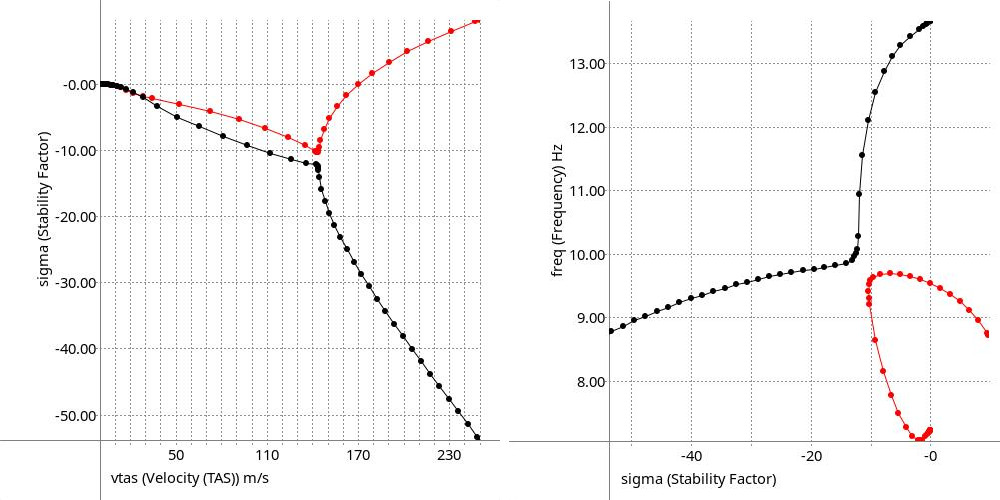
\includegraphics[height=5.5cm,width=12.5cm]{goland-vso.jpg}
%		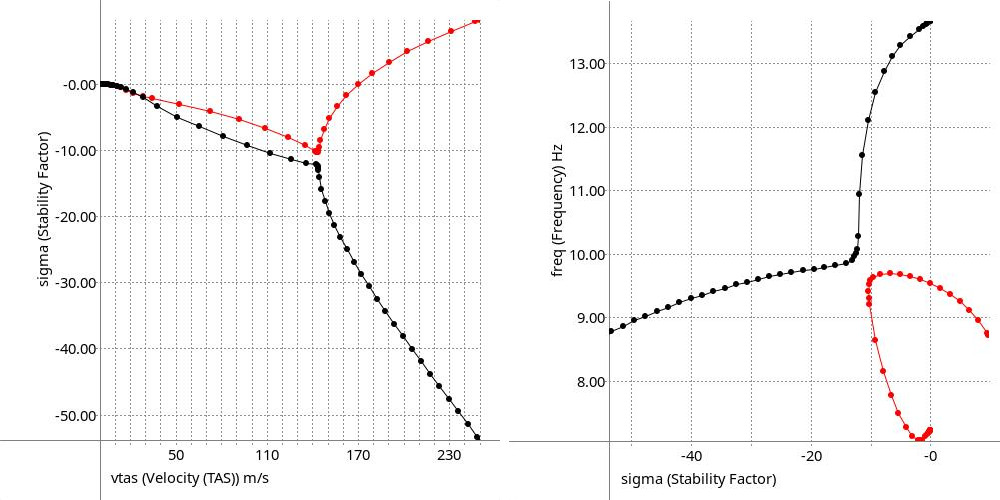
\includegraphics[height=5.5cm,width=12.5cm]{goland-vso.eps}
% 		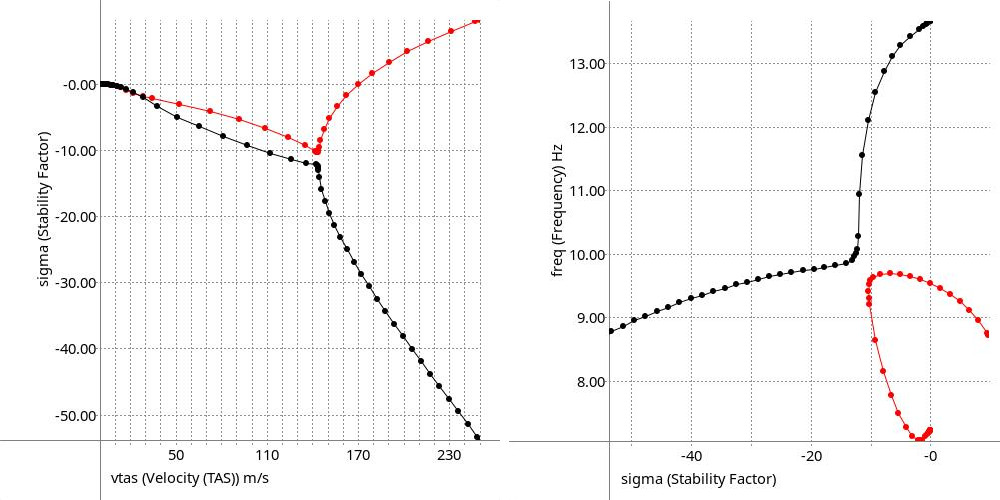
\includegraphics[height=5.5cm,width=12.5cm]{goland-vso.pdf}
	\centering
	\caption{Basic flutter (VSO) results} \label{fig:goland-vso}
\end{figure}

\subsection{Parameter variations}
The effects of certain parameters on the lowest flutter speed are then
studied by varying parameters of interest while holding $\sigma$ zero.
It is well known that 2 parameters that are important for wing flutter are
the position of the center of gravity of the wing and the position of
the aerodynamic center, relative to the elastic axis (\Figref{fig:goland-wing}).
% Results of the basic flutter analysis, shown in \Figref{fig:goland-vso},
% agree very well with \cite{goland1945flutter}.

% uses 2 structural parameterizations to demonstrate the sensitivity
% of the flutter speed to the distance from the elastic axis to the
% center of gravity and to the aerodynamic center.
\subsection{Contours}\label{ex:goland-contour}\index{contours}
A parameter, \Code{cg}, is created to give the distance from the elastic
axis to each concentrated mass; giving this name instead of a value
in the \Code{mass} section of \Cmd{fem} results in the output mass matrix
parameterized by a custom evaluation function, the source code for
which is on the current directory.
The second parameter, \Code{ac}, is created to give the distance in
the global x direction of the $3/4$ chord at the root of the doublet-lattice
grid; giving this name instead of a value in the \Code{ac} option of
the \Cmd{dlm} sub-command of the \Cmd{fem} command results in the output
unsteady aerodynamic matrix to have an interpolation parameterization
in (at least) \Code{rf} and \Code{ac}.
\par
In addition to the basic flutter results, \Code{ac} and \Code{cg} are used
to demonstrate:
\begin{enumerate}
	\item variation of flutter speed with \Code{ac}
	\item variation of flutter speed with \Code{cg}
	\item continuation-optimization of \Code{vtas} with respect to \Code{ac}
	   and \Code{cg} to get start points for
		contours\index{continuation!optimization}\index{optimization!continuation}
	\item contours of flutter speed with respect to \Code{ac} and \Code{cg}.
\end{enumerate}

\begin{figure}[ht]
		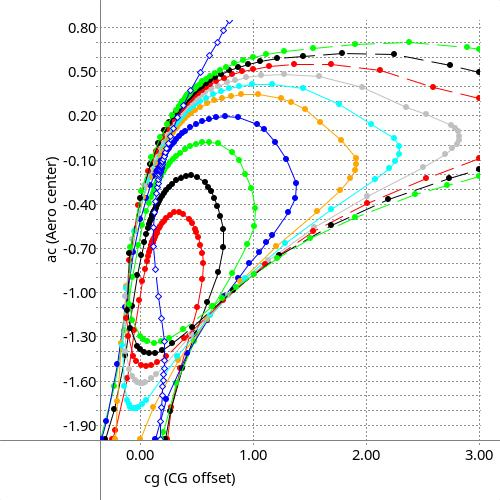
\includegraphics[height=2.5in,width=3.0in]{goland-contour.jpg}
	\centering
	\caption{Velocity contours and optimization}\label{fig:goland-contour}
\end{figure}

Plots of each of these are displayed and may be used to visualize animations
of the mode by right-clicking on the desired points.
Figure \ref{fig:goland-contour} shows the contours together with the optimization
curve used to start the contours.
% Also shown is the animated mode resulting from a right-click on a contour.

\subsection{Modal reduction}\label{ex:reduction}
\index{examples!reduction.fp}
Example file reduction.fp in the demo directory uses the Goland wing to
demonstrate reducing the model size with free vibration modes from 144
degrees-of-freedom to 10. As before, the model is built with the \Cmd{fem}
command, only with a finer grid. The mass, stiffness, and aero matrices
are fed to \Octlab along with a script that does an eigensolution and
triple products with the matrices. Two flutter solutions, one with the
full 144 dof model and the other with the reduced model show very little
difference in the 10 modes tracked.

\section{Unsteady aerodynamics: multi-variate interpolation}\label{ex:unsteady-aero}
As pointed out in \Sectref{chap:intro} \Flaps can solve flutter problems
with unsteady aerodynamics which are functions of reduced stability factor
$\bar{\sigma}$ and Mach number in addition to the usual reduced frequency
$\bar{\omega}$. Demo file \Code{dlm.fp}\index{examples!dlm.fp}
demonstrates interpolation of
the unsteady aero matrix with respect to combinations of these three
parameters. \Figref{fig:dlm-compare} shows the result of tracking
the first 2 modes using these combinations.
In this example the 2 combinations using Mach number track very differently
than the others; interpolating with Mach number results in every point on
the curve a so-called \emph{matched point}\cite{demasi2024introduction}.
\index{matched point}
\begin{figure}[ht]
		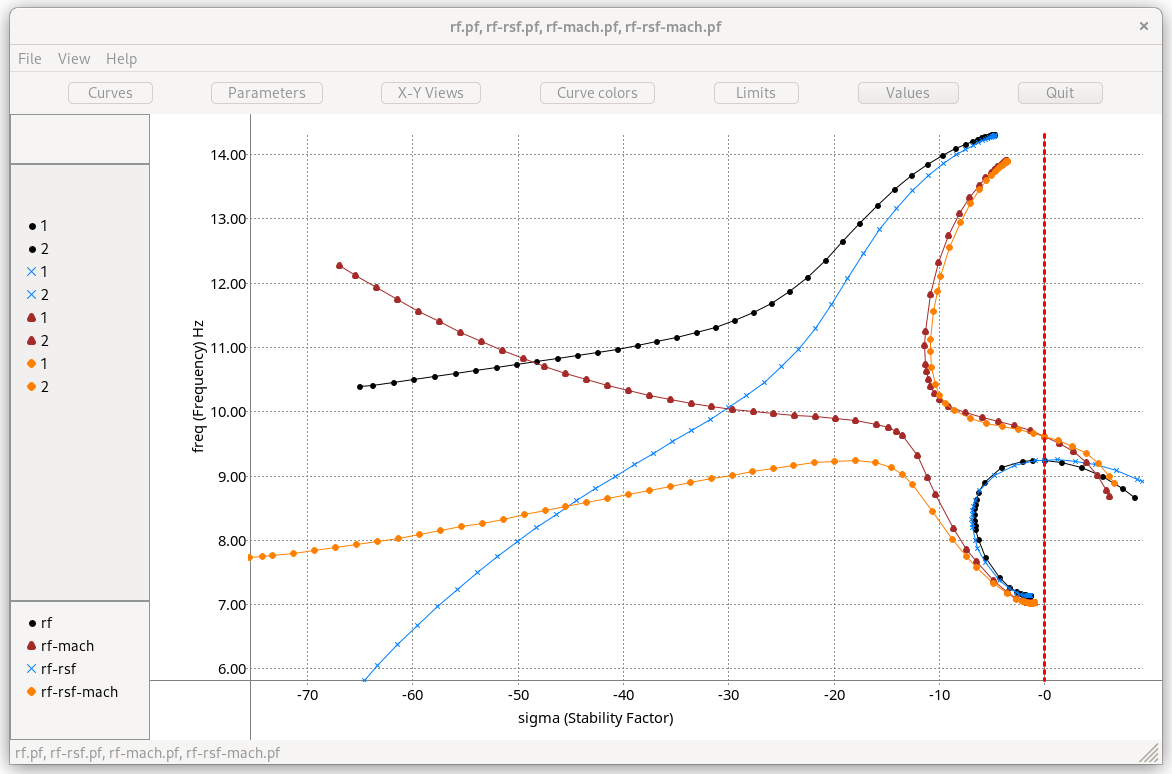
\includegraphics[height=8cm,width=12cm]{dlm-compare.png}
	\centering
	\caption{Comparison of 2 modes tracked using aerodynamics interpolated with
			combinations of 3 parameters}\label{fig:dlm-compare}
\end{figure}

% \section{Multivariate interpolation}\label{ex:dlm.fp}
% This example shows how unsteady aerodynamic matrices can be interpolated
% with respect to reduced frequency ($\bar{\omega}$),
% reduced stability factor ($\bar{\sigma}$), and Mach number ($M$).
% Using the same model as in \Sectref{ex:goland-vso} but with a collection of
% generalized aero matrices at combinations of
% 5 reduced frequencies,
% 3 reduced stability factors,
% and 3 Mach numbers, for a total of 45 matrices.

% Example file \Code{dlm.fp} in the demo directory does 4 different interpolations
% with these aero matrices:
% \begin{enumerate}
% \item interpolation with respect to reduced-frequency rf
% 	($\bar{\omega}$) at rsf=0 and mach=0.51
% \item interpolation with respect to reduced-frequency and
% 	reduced stability-factor at mach=0.51
% \item interpolation with respect to reduced-frequency and
% 	 Mach number (mach) at rsf=0
% \item interpolation with respect to reduced-frequency,
% 	 reduced stability-factor, and mach number
% \end{enumerate}

% \begin{figure}[ht]
% 		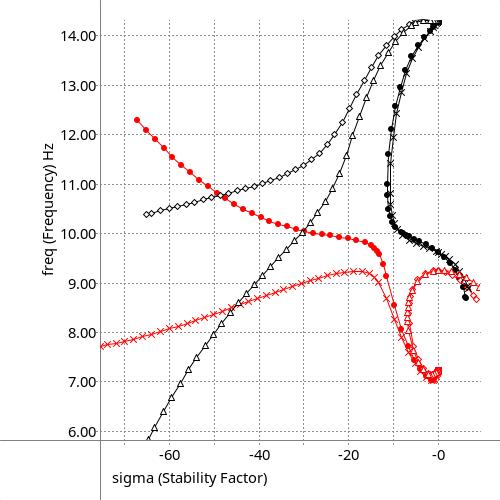
\includegraphics[height=5.5cm,width=12.5cm]{dlm.eps}
%  	\centering
%  	\caption{Aerodynamic matrix parameterizations}\label{fig:dlm}
%  \end{figure}

% Each interpolation is used in a \VSO flutter analysis
% tracking only the first 2 modes, and the
% results compared in \Figref{fig:dlm};
% evidently Mach number parameterization
% makes a bigger difference than reduced stability factor, although
% the flutter speed changes very little.

\section{Substructuring}\label{ex:substructure}
Substructuring is also used to reduce the size of models, but more
importantly for flutter is the ability to isolate parts of a structure
to accommodate control systems, nonlinearities, and parameter variations
\Sectref{sect:ss-intro}.
Example ss.fp compares 2 types of dynamic substructuring: Branch Mode
Analysis (BMA) and Component Mode Synthesis (CMS).
Whirl.fp and whirlnl.fp demonstrate BMA used for parameter variations
and freeplay nonlinearities. \Figref{fig:ss-compare} is a comparison of the
substructured models and the nodal model.
\begin{figure}[ht]
		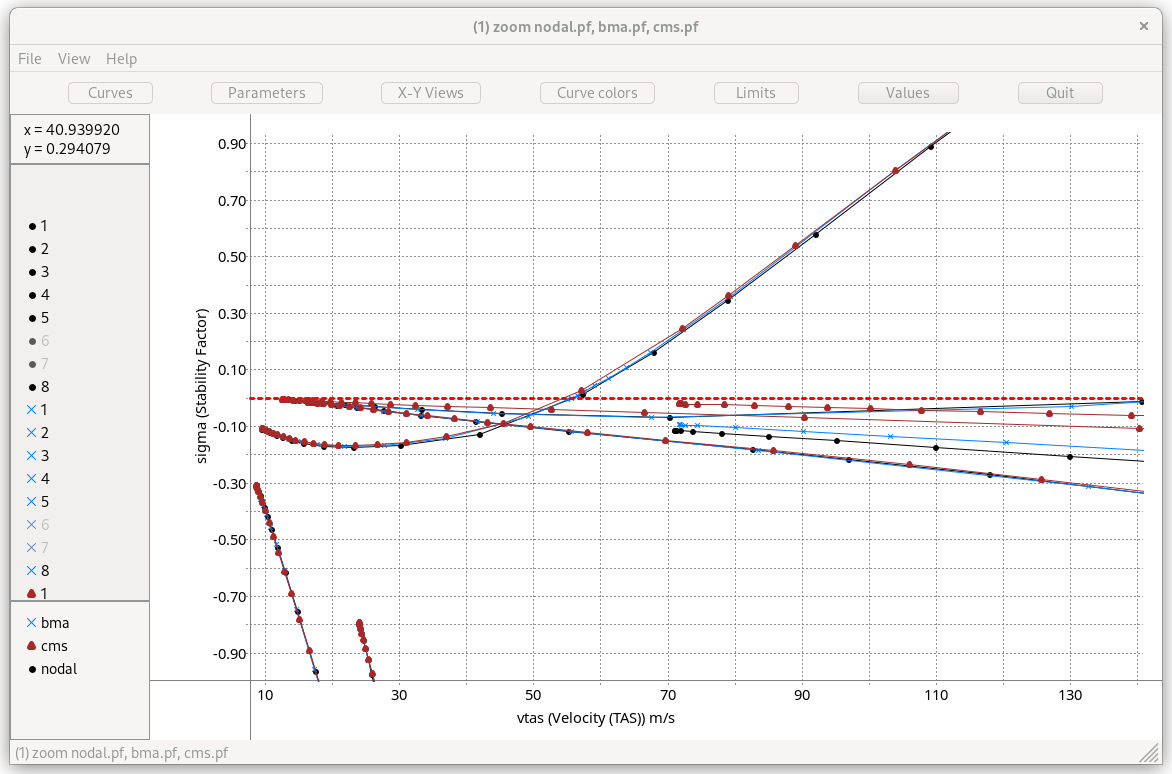
\includegraphics[height=8cm,width=12cm]{ss-compare.png}
	\centering
	\caption{Comparison of BMA, CMS, and nodal-dof models}\label{fig:ss-compare}
\end{figure}

\newpage
\section{Nonlinear flutter}\label{ex:nl1234}
\index{examples!nl[1234].fp}
\Flaps offers several ways of creating nonlinear flutter equations,
that is, parameterizing matrices with generalized-coordinate amplitudes.
The first set of problems illustrate these techniques. Next an example
shows how latent LCO can be discovered using the continuation-optimization
technique discussed in \Sectref{sect:optim}.

\subsection{Creating nonlinear equations}
Four small problems demonstrate 4 different ways of including the
same nonlinearities.
These are all based on model HA145b from the MSC/\Nastran Handbook
for Aeroelastic Analysis \cite{rodden2009msc} (which is based on
Example 9-1, p. 565 in \cite{bisplinghoff1955aeroelasticity}),
built with 10 dof.
The first 4 dof have bilinear stiffnesses (\Eqn{eqn:bilinear})
with $\delta = 0.01$ and 3 different ratios: $r_1 = r_2 = 0.5$,
$r_3 = 2$, and $r_4 = 3.5$.

The 4 files implement the bilinear describing functions using 4
different methods, with increasing levels of knowledge of \Cpp
required, but also increasing flexibility:
\begin{description}
\item[nl1.fp] builtin functions are used in equations defined in
\Code{pz} (\Sectref{opt:matrix-element}), for example
\begin{lstlisting}
   [1,1] *= bilinear(0.01, 0.5, 1)
\end{lstlisting}
multiplies the [1,1] term by the bilinear describing function with
$\delta=0.01$, $r = 0.5$, and $|\hat{q}_1|$.

\item[nl2.fp] a custom function which does the same multiplication
calling builtin function \Code{df::freeplay}

\item[nl3.fp] uses custom functions to call local custom functions
called \Code{freeplay} and \Code{bilinear}

\item[nl4.fp] a custom function which uses describing functions
created automatically when 3 functions written in \Cpp are included as
a section in the flaps input file. The 3 functions must have these names and
calling arguments:
	\begin{lstlisting}
vector<double> df_qs(const vector<double>& params)

double df_fq(double y, const vector<double>& params)

Interp* df_interp(const string& iid, const vector<double>& params,
    const vector<double>& qs, const vector<double>& fs)
	\end{lstlisting}
%%	returns a vector with the desired amplitudes
%%	returns the factor which when multiplied by $\Matrix{K}\Vector{y}$ gives the force at the nonlinearity
%% returns a pointer to a new Interp object containing one or more interpolants

\end{description}


\subsection{Latent limit cycles}\label{ex:latent}\index{LCO!latent}
Example problem \Code{latent.fp} shows the discovery of limit-cycles including
three that do not go unstable when \Gc norm ($\eta$) is zero (latent LCO).
\index{nonlinear flutter}\index{LCO!latent}
The model is a simple model of a twin-engine airplane with several nonlinearities:
\begin{itemize}
	\item freeplay on elevator, rudder, and ailerons
	\item bilinear stiffness on nacelle struts
\end{itemize}
The study of limit-cycles involves these \Cmd{flut} processes:
\begin{description}
	\item[\Code{vso}] a \VSO search for flutter speeds with \Gc norm zero,
	   i.e. linear flutter points.
	\item[\Code{voe0}] starting from flutter speeds in \Code{vso}, varying
	   $v$, $\omega$, and $\eta$. These \Lco curves show that some linear
		flutter points have limit-cycles extending below their linear flutter speed.
	\item[\Code{soe}] variation in $\sigma$ with $\eta$ to locate $\sigma=0$ points
	\item[\Code{voe1}] starting from points in \Code{soe} where $\sigma=0$ to
	   trace \Lco curves. Some of these \Lco curves do not extend to $\eta=0$ so
		they were not found in \Code{voe0}.
	\item[\Code{vsoe}] like \Code{soe}, a \Code{vsoe} process varies $\sigma$,
		$\omega$, and $\eta$ searching for $\sigma=0$ targets. In addition, a
		\Code{vsoe} process allows $V$ to vary while guiding the curve towards
		increasing $\sigma$.
	\item[\Code{voe2}] starting from points in \Code{vsoe} where $\sigma=0$ to
		trace \Lco curves.
\end{description}
\Figref{fig:lco_screen} shows a few latent LCO boundaries discovered using
this set of \Cmd{flut} solutions. The stability of the LCO is indicated by
a change in the color of the curve. A red dot indicates a point that was
clicked on to bring up the animated mode.

\begin{figure}[ht]
		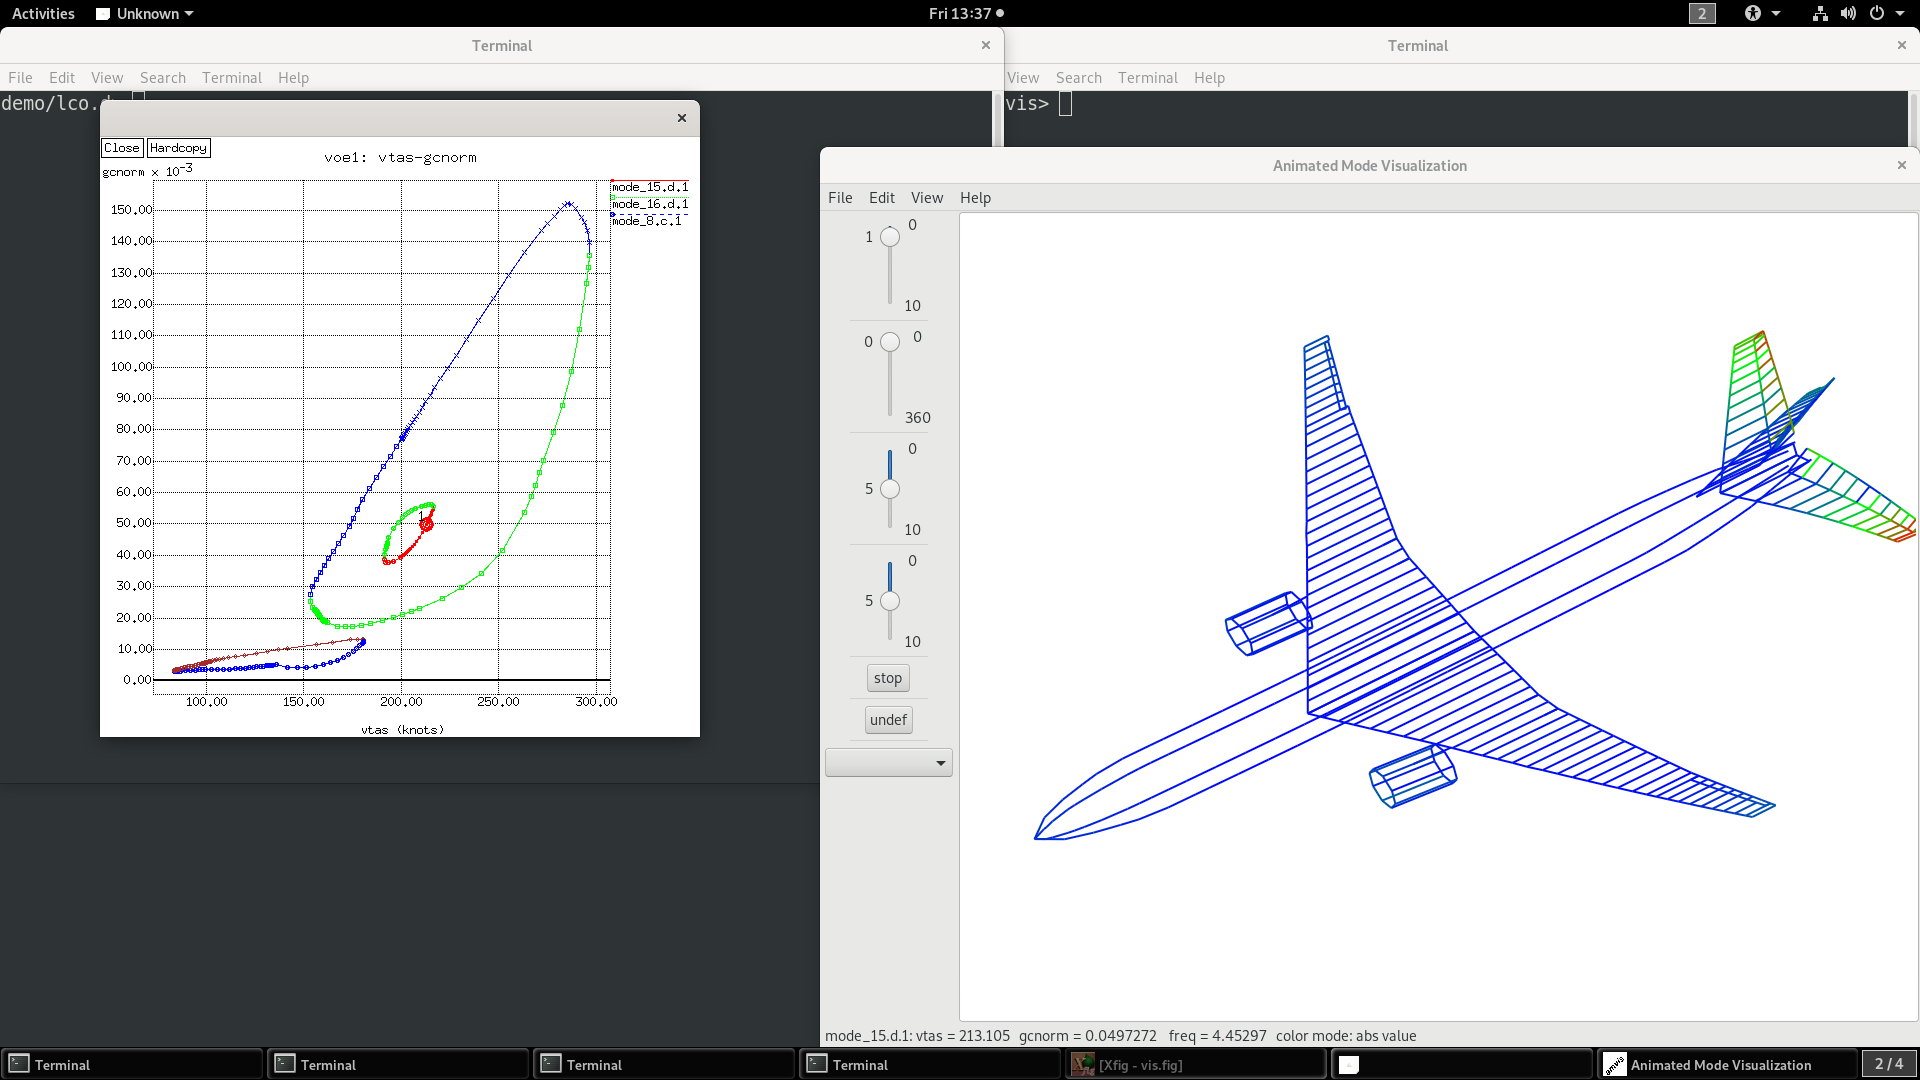
\includegraphics[height=3in,width=4.8in]{lco_screen.png}
	\centering
	\caption{Latent LCO}\label{fig:lco_screen}
\end{figure}

\newpage
\section{Controls Equations}\label{ex:controls}
\index{examples!controls.fp}
Using the same airplane model as in \Sectref{ex:latent}, \Code{controls.fp} uses
a custom function to describe a nonlinear control-system.
The nonlinearities are in the gain, phase, and sensors.
Capabilities demonstrated include
\begin{itemize}
	\item using \Cmd{octlab} to extract 2 rows of the \Code{gctransform}
	    matrix to use in sensor equations
	\item a section of \Cpp code describing the controls equations in
	   the \Tmatrix.
	\item a \VSO analysis varying reduced-frequency instead of \Code{vtas}
	   so that every solution point produced is within the limits of
		reduced-frequency. The \Tmatrix\ is included but with \Code{gcnorm=0}
		it does not affect the solution.
	\item a \VSO analysis including the controls equations with \Code{gcnorm=0}
	   but with a spec, \Code{linearize} which is passed to the
		controls function where the equations are linearized. With these
		linearized controls equations there is a small increase in flutter speed.
	\item a \VSOE analysis to see the effect of increasing the oscillation
	   amplitude on $\sigma$, that is, a search for LCO by driving $\sigma$
		towards zero by a continuation-optimization \index{continuation!optimization}
		with \VSOE.
	\item gain and phase variations to see their influence on linear
	   flutter speed
	\item a gain-phase-frequency-velocity optimization to get start
	   points for velocity contours
	\item gain-phase variations at a few velocities start from the optimization,
	   giving velocity contours.
\end{itemize}

\begin{figure}[ht]
		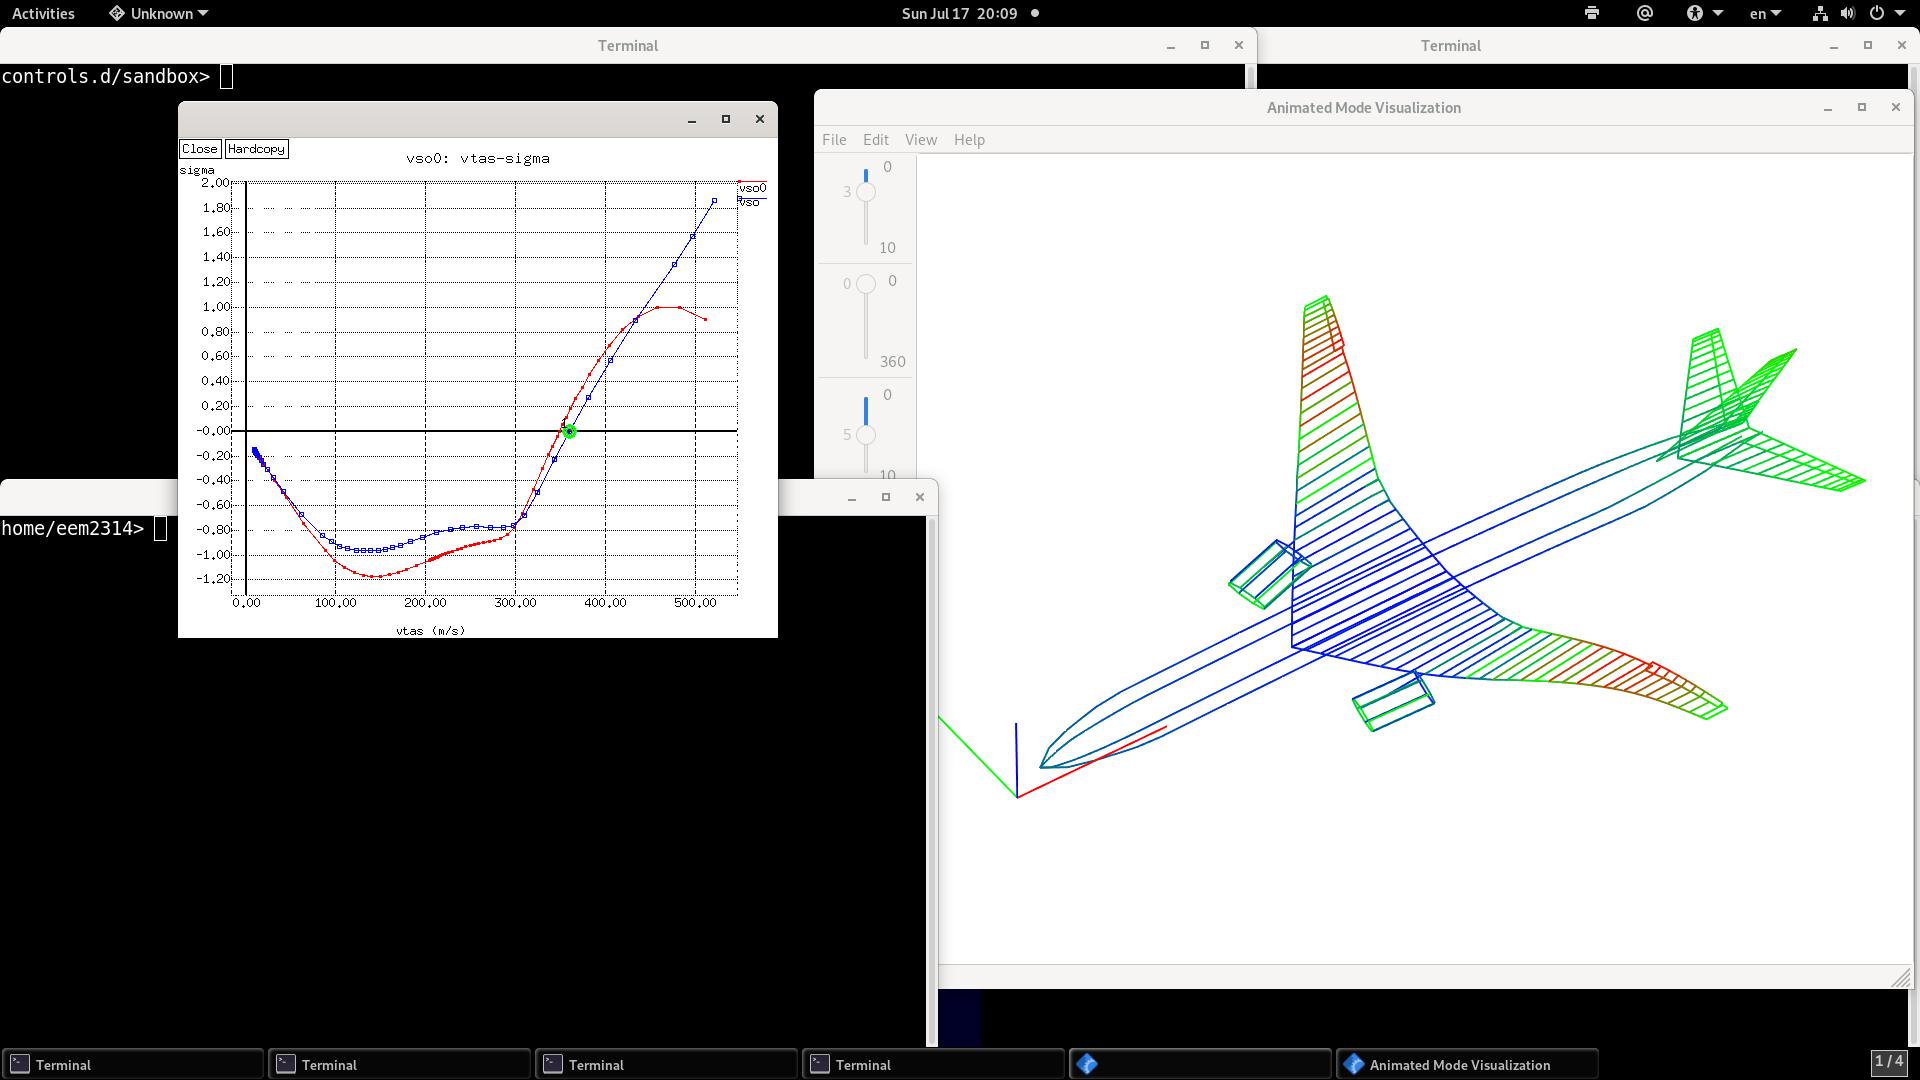
\includegraphics[height=2in,width=3.0in]{controls_vso.png}
	\centering
	\caption{\Code{controls.fp} closed- and open-loop flutter}\label{fig:controls_vso}
\end{figure}

\newpage
\section{Whirl flutter}\label{ex:whirl}\index{whirl flutter}\index{flutter!whirl}
\index{examples!reed.fp}
\index{examples!whirl.fp}
Three example problems illustrate whirl flutter:
\Code{reed.fp} demonstrates whirl flutter on a simple rigid propeller
to validate the \Flaps implementation of \cite{reed1961analytical},
% in \Figref{fig:whirl-gaf},
\Code{whirl.fp} is the Goland wing with 2
propellers attached, and \Code{whirlnl.fp} is the same but with freeplay
on the propeller mounts. For these a gyro matrix is created with the \Cmd{gyro}
command (\Sectref{ref:fem-gyro}), and
unsteady propeller aerodynamics are from \cite{reed1961analytical},
summarized in \Sectref{sect:whirl-aero}, and are implemented
in a custom evaluation function created on the current working directory
(\Code{pgaffcn.cpp}).

The frequency in a whirl flutter analysis is the rate
at which the spinning shaft is precessing about the resting
axis; this precessional\index{precession} motion can be expressed in revolutions
per minute (rpm) instead of Hertz by changing the definition
of frequency:
\begin{lstlisting}
   parameter{freq(Precessional spin rate)[0:10]<radps2rpm>}
\end{lstlisting}
where the builtin constant \Code{radps2rpm} is used here to
change the global definition to
\Code{freq[0:10](Precessional spin rate)<9.5493 rpm/(rad/s)>}

Figures \ref{fig:whirl-vso}, \ref{fig:beta}, and \ref{fig:whirl-lbar}
show some results using this aerodynamic model on the simple rigid
propeller in \Code{reed.fp}.
\begin{figure}[hbt!]
	\includegraphics[height=8.0cm,width=8.0cm]{whirl-vso.eps}
%	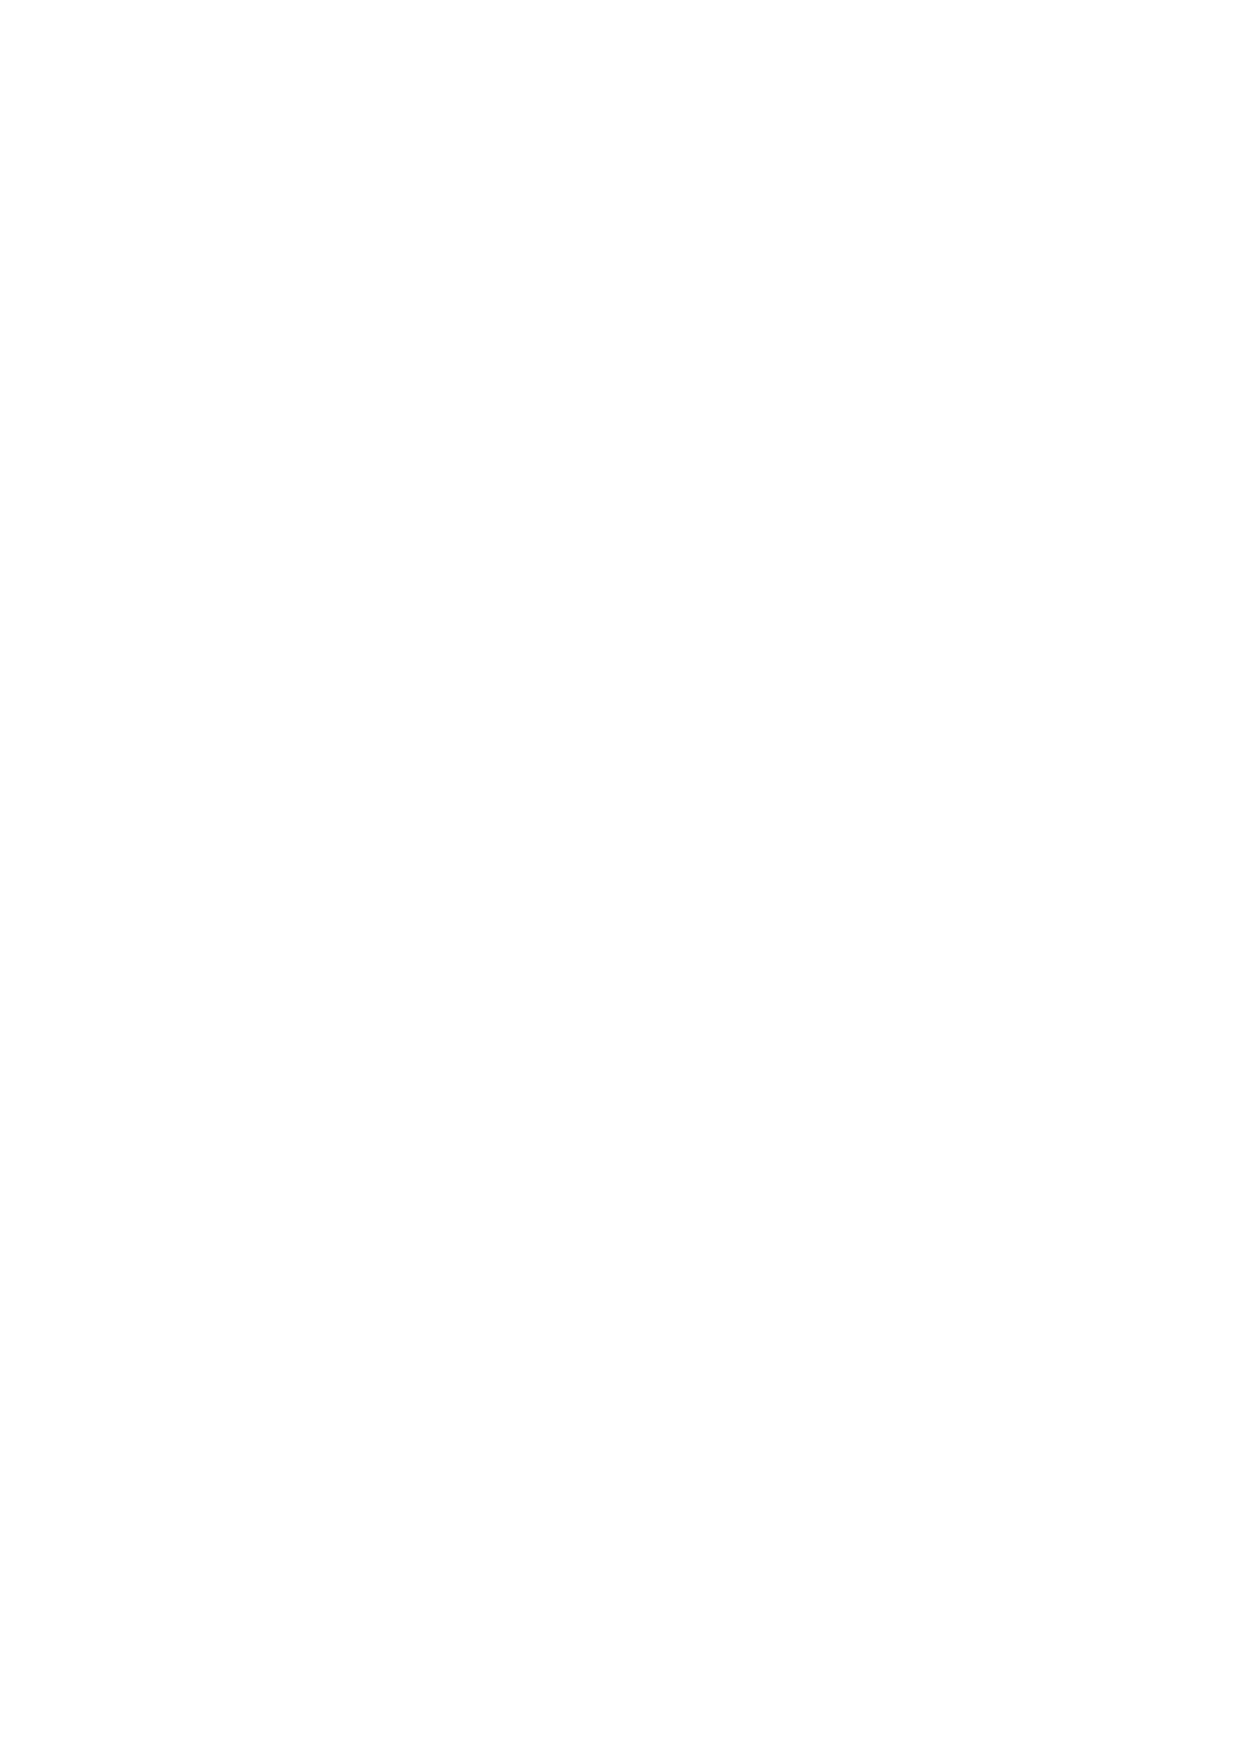
\includegraphics[height=8.0cm,width=8.0cm]{whirl-vso.pdf}
	\centering
	\caption{V-$\sigma$ at 100 rpm}\label{fig:whirl-vso}
\end{figure}

\begin{figure}[hbt!]
	\includegraphics[height=8.0cm,width=8.0cm]{beta.eps}
\centering
\caption{Variation of flutter speed with blade angle}\label{fig:beta}
\end{figure}

\begin{figure}[hbt!]
	\includegraphics[height=13.0cm,width=8.0cm]{whirl-lbar.eps}
%	\includegraphics[height=13.0cm,width=8.0cm]{whirl-lbar.pdf}
\centering
\caption{Variation of flutter speed and frequency with $l/r$}\label{fig:whirl-lbar}
\end{figure}

\clearpage
\pagebreak

\section{Bifurcation}\label{ex:bifurcation}
\index{bifurcation!example}
Bifurcation, usually associated with nonlinear systems, can occur in
linear flutter analyses, a reminder that even though a flutter analysis
is termed linear because it is independent of generalized coordinate
amplitudes, it is still nonlinear in parameters such as velocity and frequency
\cite{meyer2015continuation}.

Example problem \Code{bif.fp} demonstrates bifurcation in the Goland wing
by changing the moment of inertia about the y axis slightly, causing a
mode to bifurcate, with one branch returning to zero velocity and the
other becoming neutrally stable, as shown in \Figref{fig:bifurcation}.

\begin{figure}[h!]
		\includegraphics[height=7.0cm,width=8.5cm]{bif.eps}
%		\includegraphics[height=7.0cm,width=8.5cm]{bif.pdf}
	\centering
	\caption{Bifurcation in the Goland wing}\label{fig:bifurcation}
\end{figure}

\newpage
\chapter{Appendix}\label{chap:appendices}

\section{Rational-Function Approximation}\label{sect:rfa-theory}
\par
\index{s-plane approximation}
\index{RFA}
\index{aerodynamics!approximation}
The \Cmd{pz} command can approximate generalized
unsteady aerodynamic matrices using a rational-function
approximation often referred to as \Newterm{s-plane approximation}
aerodynamics, even though the approximation is done
with respect to complex reduced-frequency $\bar{s} = s/V$,
not the Laplace variable $s = \sigma + i\omega$.
This approximation, due to Roger \cite{roger1977airplane},
uses a least-squares fit of a rational-function polynomial
to a set of complex matrices. Given a set of $m$
unsteady aero matrices at various values of complex
reduced frequency $\bar{s}$\footnote{this procedure is usually written
in terms of only the imaginary part of $\bar{s}$, the reduced-frequency; here
we allow for applying it to Laplace-domain aerodynamic matrices}.
\begin{equation}
\Matrix{A}_k = \Matrix{A}(\bar{s}_k) = \left[A_{ij,k}\right]
			\hspace{5mm} (k = 1, m) \; \; \in \mathbb{C}^{n \times n},
\end{equation}
approximate $\Matrix{A}$ with an analytic function of $\bar{s}$ and a set of
$\ell$ positive, real \emph{lag roots} $\beta_i, i=1,\ell$.
Roger's approximation to the aero matrix has the form
\begin{equation}
  \Matrix{A}(\bar{s}) \approx \Matrix{R}_0 + \bar{s}\Matrix{R}_1 + \bar{s}^2 \Matrix{R}_2 +  \sum_{l=1}^{\ell} \frac{\bar{s}}{\bar{s} + \beta_l} \Matrix{R}_{l+2}
\end{equation}
where the $\ell + 3$ matrices
$\Matrix{R}_0, \Matrix{R}_1, \ldots, \Matrix{R}_{\ell+2}$ are real.
Each element
\begin{displaymath}
R_{ij,0}, R_{ij,1}, \ldots, R_{ij,\ell+2}
\end{displaymath}
is determined by $2m$ equations, comprising the real and imaginary parts
of the $m$ $\Matrix{A}$ matrices:
\begin{eqnarray}
	\Re(R_{ij,0} + \bar{s}_k R_{ij,1}
  		+ \bar{s}_k^2 R_{ij,2} +  \sum_{l=1}^{\ell} \frac{\bar{s}_k}{\bar{s}_k +
			\beta_l} R_{ij,l+2}) &=& \Re(A_{ij,k}) \nonumber	\\
	\Im(R_{ij,0} + \bar{s}_k R_{ij,1}
  		+ \bar{s}_k^2 R_{ij,2} +  \sum_{l=1}^{\ell} \frac{\bar{s}_k}{\bar{s}_k +
			\beta_l} R_{ij,l+2}) &=& \Im(A_{ij,k})	\nonumber
\end{eqnarray}
% \begin{eqnarray}
% 	\Re(\Matrix{R}_0 + \bar{s}_k\Matrix{R}_1
%   		+ \bar{s}_k^2 \Matrix{R}_2 +  \sum_{i=1}^{\ell} \frac{\bar{s}_k}{\bar{s}_k +
% 			\beta_i} \Matrix{R}_{i+2}) &=& \Re(\Matrix{A}_k) \nonumber	\\
% 	\Im(\Matrix{R}_0 + \bar{s}_k\Matrix{R}_1
%   		+ \bar{s}_k^2 \Matrix{R}_2 +  \sum_{i=1}^{\ell} \frac{\bar{s}_k}{\bar{s}_k +
% 			\beta_i} \Matrix{R}_{i+2}) &=& \Im(\Matrix{A}_k)
% \end{eqnarray}
from which we can determine the $(i,j)$ elements of the $\Matrix{R}$ matrices:
$(\ell+3)$ unknowns. Provided $2m > \ell+3$ these equations are overdetermined
and can be solved by least-squares:
\begin{equation}
\Matrix{S}\Vector{x} = \Vector{b}
\end{equation}
where
\begin{displaymath}
\Matrix{S} = \left[
\begin{array}{cccccc}
1 & \Re(\bar{s}_1) & \Re(\bar{s}_1^2) & \Re(\frac{\bar{s}_1}{\bar{s}_1 + \beta_1}) & \ldots & \Re(\frac{\bar{s}_1}{\bar{s}_1 + \beta_{\ell}}) \\
0 & \Im(\bar{s}_1) & \Im(\bar{s}_1^2) & \Im(\frac{\bar{s}_1}{\bar{s}_1 + \beta_1}) & \ldots & \Im(\frac{\bar{s}_1}{\bar{s}_1 + \beta_{\ell}}) \\
1 & \Re(\bar{s}_2) & \Re(\bar{s}_2^2) & \Re(\frac{\bar{s}_2}{\bar{s}_2 + \beta_1}) & \ldots & \Re(\frac{\bar{s}_2}{\bar{s}_2 + \beta_{\ell}}) \\
0 & \Im(\bar{s}_2) & \Im(\bar{s}_2^2) & \Im(\frac{\bar{s}_2}{\bar{s}_2 + \beta_1}) & \ldots & \Im(\frac{\bar{s}_2}{\bar{s}_2 + \beta_{\ell}}) \\
  &          &            &                                & \ddots &                           \\
1 & \Re(\bar{s}_m) & \Re(\bar{s}_m^2) & \Re(\frac{\bar{s}_m}{\bar{s}_m + \beta_1}) & \ldots & \Re(\frac{\bar{s}_m}{\bar{s}_m + \beta_{\ell}}) \\
0 & \Im(\bar{s}_m) & \Im(\bar{s}_m^2) & \Im(\frac{\bar{s}_m}{\bar{s}_m + \beta_1}) & \ldots & \Im(\frac{\bar{s}_m}{\bar{s}_m + \beta_{\ell}}) \\
\end{array}
\right]	\hspace{3mm} \in \mathbb{R}^{2m\times \ell+3}
\end{displaymath}

\begin{displaymath}
\Matrix{x} = \left\{
\begin{array}{c}
R_{ij,0} \\
R_{ij,1}  \\
\ddots  \\
R_{ij,\ell+2}
\end{array}
\right\}		\hspace{3mm} \in \mathbb{R}^{\ell+3}
\end{displaymath}

\begin{displaymath}
 \Matrix{b} =
\left\{
\begin{array}{c}
\Re(A_{ij,1}) \\
\Im(A_{ij,1}) \\
\Re(A_{ij,2}) \\
\Im(A_{ij,2}) \\
\ddots \\
\Re(A_{ij,m}) \\
\Im(A_{ij,m})
\end{array}
\right\}		\hspace{3mm} \in \mathbb{R}^{2m}
\end{displaymath}
The coefficient matrix $\Matrix{S}$ is the same for all elements of the
$\Matrix{R}$ matrices so all $n^2$ elements can be computed simultaneously
with, for example Lapack routine \Code{DGELSS} \cite{anderson1999lapack}.

\section{Time domain formulation}\label{sect:timedomain}
\index{time domain}
Most numerical methods for solving systems of ordinary require the
problem to be a set of first-order equations
sometimes referred to as \Newterm{state space} form.
Formulating flutter equations in the time domain is trivial except for unsteady
aerodynamics. Unsteady aerodynamics are commonly in the frequency domain,
functions of reduced frequency and possibly reduced stability factor (\Code{rsf}) and
Mach number (\Code{M}); if dependence on \Code{rsf} and \Code{M} are not allowed,
a rational-function approximation is a way to convert from the frequency domain to the
time domain; Roger's approximation\cite{roger1977airplane}
(\Sectref{sect:rfa-theory}) is a rational function
in terms of \Code{s}, \Code{V} and real matrices, so the flutter equation can
be written in terms of \Code{s}, \Code{V} and real matrices, then converted
to the time domain with the inverse Laplace transform with \Code{s} as the Laplace
variable.

\subsection{First-Order Time-domain Equations}\label{sect:statespace}
To allow for unsteady aerodynamics
we start with the characteristic equations of motion
(frequency domain), cast them into a set of first-order equations
(in the Laplace variable \Code{s}, then convert to the time domain with the inverse
Laplace transform.

Without structural damping and user-defined matrix ($\Matrix{T}$),
and aerodynamics at a fixed Mach number,\Eqn{eqn:flut} is
% \begin{equation}\label{eqn:td-base}
% 	\left[ s^2 \Matrix{M} + s \left(\Matrix{G} + \Matrix{V} \right)
% 	+ \Matrix{K} - q \Matrix{Q}(\bar{s},M) \right] \Vector{y} = \Vector{0}
% \end{equation}
\begin{equation}
	\left[ s^2 \Matrix{M} + s \Matrix{G} + s \Matrix{V} +
		\Matrix{K} - q \Matrix{A} (\bar{s}) \right] \hat{\Vector{y}}
		= \hat{\Matrix{D}}\hat{\Vector{y}} = \Vector{0} \; \; \in \mathbb{C}^{n_e}, \nonumber
\end{equation}
The unsteady aerodynamic matrix is assumed to be a rational-function approximation
in the form (\Sectref{sect:rfa-theory})
\begin{equation}
\Matrix{A}(\bar{s}) \approx \Matrix{R}_0 + \bar{s}\Matrix{R}_1 + \bar{s}^2 \Matrix{R}_2 +  \sum_{i=1}^{m} \frac{\bar{s}}{\bar{s} + \beta_i} \Matrix{R}_{i+2}	\nonumber
\end{equation}
created using the RFA approximation from the \Cmd{pz} command (\Sectref{ref:pz}).

Introducing m new variables $\Vector{x}_{i+1}$ ($i=1,m$), one for each $\beta$:
\begin{equation}
	\Vector{x}_{i+1} = \frac{\bar{s}}{\bar{s} + \beta_i} \hat{\Vector{y}}
		= \frac{sb}{sb + V \beta_i} \hat{\Vector{y}}		\nonumber
\end{equation}
so that
\begin{equation} \label{eqn:beta-s}
	s \Vector{x}_{i+1} = s \hat{\Vector{y}} - \frac{V}{b} \beta_i \Vector{x}_{i+1}
\end{equation}
and the equations of motion become
\begin{eqnarray}
	\hat{\Matrix{D}}\hat{\Vector{y}} &=& \Vector{0} \nonumber \\
	\hat{\Matrix{D}} &=& s^2 \left[ \Matrix{M} - q\left(\frac{b}{V}\right)^2 \Matrix{R}_2 \right]
		+ s \left[ \Matrix{G} + \Matrix{V} - q\frac{b}{V} \Matrix{R}_1 \right] \nonumber \\
		& & + \Matrix{K} - q \Matrix{R}_0 - q \sum_{i=1}^{m} \Matrix{R}_{i+2} \Vector{x}_{i+1} \nonumber
\end{eqnarray}
or to allow for zero velocity
\begin{eqnarray}
	\hat{\Matrix{D}} &=& s^2 \left[ \Matrix{M} - \frac{\rho b^2}{2}\Matrix{R}_2 \right]
		+ s \left[ \Matrix{G} + \Matrix{V} - \frac{\rho V b}{2} \Matrix{R}_1 \right] \nonumber \\
		& & + \Matrix{K} - q \Matrix{R}_0 - q \sum_{i=1}^{m} \Matrix{R}_{i+2} \Vector{x}_{i+1}
\end{eqnarray}
Now let
\begin{equation}
\Matrix{P} = \left[\Matrix{M} - \frac{\rho b^2}{2}\Matrix{R}_2\right]^{-1}		\nonumber
\end{equation}
so that
\begin{eqnarray}
	\Vector{P}\hat{\Vector{D}}\hat{\Vector{y}} & = & \Vector{0} \nonumber \\
					 & = & \left[ s^2 + s\Matrix{P} \left(\Matrix{G} + \Matrix{V}
						- \frac{\rho V b}{2}\Matrix{R}_1 \right) + \Matrix{P} \left( \Matrix{K}
						- q \Matrix{R}_0 \right) \right] \hat{\Vector{y}} \nonumber \\
						& & - q \sum_{i=1}^{m} \Matrix{PR}_{i+2} \Vector{x}_{i+1} \nonumber
\end{eqnarray}
or
\begin{eqnarray}\label{eqn:eom-fd}
	s^2\hat{\Vector{y}} &=& -s \Matrix{P} \left(\Matrix{G} + \Matrix{V} -
				\frac{\rho V b}{2}\Matrix{R}_1 \right) \hat{\Vector{y}} -
				\Matrix{P} \left(\Matrix{K} - q\Matrix{R}_0 \right)\hat{\Vector{y}} \nonumber \\
				& & + q \sum_{i=1}^{m} \Matrix{PR}_{i+2} \Vector{x}_{i+1}
\end{eqnarray}
Applying the inverse Laplace transform,
$s\hat{\Vector{y}} \rightarrow \dot{\Vector{x}_1}$
and $s^2\hat{\Vector{y}} \rightarrow \ddot{\Vector{x}_1}$
where $\Vector{x}_1$ is a vector of discrete physical displacements in the time domain,
\Eqn{eqn:eom-fd} becomes
% \footnote{note notation change from $\Vector{q}$ to $\Vector{x}_1$ to be consistent with \Sectref{chap:theory}}.
\begin{equation}
	\ddot{\Vector{x}_1} = -\Matrix{P} \left( \Matrix{G} + \Matrix{V} -
        \frac{\rho V b}{2}\Matrix{R}_1 \right) \dot{\Vector{x}_1} -
        \Matrix{P} \left(\Matrix{K} - q\Matrix{R}_0 \right)\Vector{x}_1 + 
		  q \sum_{i=1}^{m} \Matrix{PR}_{i+2} \Vector{x}_{i+1}		\nonumber
\end{equation}
and \Eqn{eqn:beta-s} becomes
\begin{equation}
	\Vector{\dot{x}}_{i+1} = \Vector{\dot{x}_1} - V \beta_i \Vector{x}_{i+1}
			\hspace{0.5cm}(i = 1, m)	\nonumber
\end{equation}
which together can be written in $n_t = (m+2)n$ time-domain, real first-order ordinary differential
equations (state-space) form:
\begin{equation}\label{eqn:statespace}
	\Vector{\dot{x}}(t) = \Vector{f}(\Vector{x},t) = \Matrix{F}(\Vector{x})\Vector{x}(t)
\end{equation}
where
\begin{equation}
	\Vector{x} = \left\{ \begin{array}{c}
                      \Vector{x}_1 \\
                      \dot{\Vector{x}}_1 \\
                      \Vector{x}_2 \\
                      \Vector{x}_3 \\
                      \ldots \\
                      \Vector{x}_{m+1}
                      \end{array} \right\} \;\; \in \mathbb{R}^{n_t}\notag
\end{equation}
and
\begin{equation}
	\Matrix{F} = \left[ \begin{array}{cccccc}
							\Matrix{0}  &  \Matrix{I}   &    \Matrix{0}    &    \Matrix{0}    &    & \Matrix{0} \\
							- \Matrix{P} ( \Matrix{K} - q \Matrix{R}_0 ) &  - \Matrix{P} \left( \Matrix{G} + \Matrix{V}
							- \frac{\rho V b}{2} \Matrix{R}_1 \right)   &  q \Matrix{PR}_3 & q \Matrix{PR}_4    & \vdots  & q \Matrix{PR}_{m+2} \\
							\Matrix{0}  &  \Matrix{I}   &  -V \beta_1 \Matrix{I}    &    \Matrix{0}    &    & \Matrix{0} \\
							\Matrix{0}  &  \Matrix{I}   & \Matrix{0} &  -V \beta_2 \Matrix{I}    &    & \Matrix{0} \\
							&  \ldots &   &  & \ddots  & \\
							\Matrix{0}  &  \Matrix{I}   & \Matrix{0} &  \Matrix{0}    &    & -V \beta_m \Matrix{I}
					\end{array} \right] \notag
\end{equation}
is an $(n_t,n_t)$ real matrix.
Equation \ref{eqn:statespace} has been written with $\Vector{F}$ as a
function of $\Vector{x}$ to allow for nonlinearities in any of the matrices,
for example freeplay in stiffness terms.

The trivial solution $\Vector{x}=\Vector{0}$ is an equilibrium since there
$\dot{\Vector{x}} = \Vector{0}$; the stability of a trivial equilibrium is determined
by the eigenvalues of
\begin{equation}
\frac{\partial\Vector{f}}{\partial\Vector{x}} = \Matrix{J} =
	\Matrix{F} + \frac{\partial\Vector{F}}{\partial\Vector{x}}\Vector{x}
\end{equation}
These ($n_t$) eigenvalues are complex with stability determined by the real part:
negative means stable, positive unstable.
At low velocities an airplane will (hopefully) be stable; monitoring the eigenvalues
with increasing velocity might encounter a Hopf bifurcation \cite{seydel1988equilibrium},
where the real part goes from negative to positive, corresponding to the velocity in the
frequency domain where $\sigma$ does the same, the critical or lowest flutter speed.

If $\Matrix{F}$ is a function of $\Vector{x}$ a Hopf bifurcation leads to limit-cycle
oscillations at non-zero $\Vector{x}$.
Starting from the bifurcation a continuation process can be used to trace
the curve of limit-cycle oscillations, by increasing the amplitude and allowing
velocity and the imaginary part of the eigenvalue to vary with the real part
of the eigenvalue set to zero.

% That is the main reason for including this section: to allow tracing equilibriums
% determined by solutions to
% \begin{equation}
% $	\Vector{\dot{x}} = \Matrix{F}(\Vector{x})\Vector{x} = \Vector{0}$.
% \end{equation}
% These equilibriums points can be traced with continuation, monitoring for
% bifurcation. Nonlinear structures may encounter Hopf bifurcations
% \cite{seydel1988equilibrium} indicating limit cycle oscillation. The goal is
% to assess the accuracy of describing function approximations in the frequency
% domain by comparing with solutions in the time domain.

% \section{Programming Details}\label{sect:programming}
% The \Flaps \Cmd{flut} command, as is the rest of \Flaps, is written in \Cpp
% making several features possible that either speed up execution or add
% solution capabilities.

% ------------------------------------------------------------------
\section{State-space controls equations}\label{sect:abcd-conversion}
\index{controls equations!lti}\index{LTI control system!conversion}
A linear, time-invariant control system can be represented by the
block diagram in \Figref{fig:abcd-block}
\begin{figure}[ht]
		\includegraphics[height=6.5cm,width=12cm]{lti-block.eps}
	\centering
	\caption{Linear control system block diagram}\label{fig:abcd-block}
\end{figure}
and mathematically in time-domain state-space form
(\cite{brogan1982modern} p. 172):
\begin{eqnarray}
\dot{\Vector{v}} &=& \Vector{Av} + \Vector{Bu_i} 	\nonumber \\
\Vector{u_o} &=& \Vector{Cv} + \Vector{Du_i}	\nonumber
\end{eqnarray}
where $\Vector{v}$ is an $n_s$-vector of states, $\Vector{u_i}$
is an $n_i$ -vector of inputs, $\Vector{u_o}$ is an $n_o$-vector of outputs,
and the matrices have dimensions:
\begin{eqnarray*}
\Matrix{A} & : & (n_s, n_s) \\
\Matrix{B} & : & (n_s, n_i) \\
\Matrix{C} & : & (n_o, n_s) \\
\Matrix{D} & : & (n_o, n_i)
\end{eqnarray*}
If there are input and output time delays the controls equations can be written
in the frequency domain
\index{time delays}
\begin{eqnarray}\label{eqn:abcd1}
s\Vector{v} &=& \Vector{Av} + \Vector{BGu_i} \\
\Vector{u_o} &=& \Vector{HCv} + \Vector{HDGu_i} \label{eqn:abcd2}
\end{eqnarray}
where
\begin{eqnarray}
\Matrix{G} &=& \left[ \begin{array}{ccc}
\ddots &           &        \\
       & g_i e^{-st_i} &        \\
       &           & \ddots
\end{array}
\right] \;\; \in \mathbb{C}^{n_i \times n_i}	\nonumber	\\
\Matrix{H} &=& \left[ \begin{array}{ccc}
\ddots &           &        \\
       & h_j e^{-st_j} &        \\
       &           & \ddots
\end{array}
\right]	\;\; \in \mathbb{C}^{n_o \times n_o}	\nonumber
\end{eqnarray}
are diagonal matrices, $g_i$ and $t_i$ are the (complex) gain
and time delay associated with the $i^{th}$ input channel, and
$h_j$ and $t_j$ are the (complex) gain and time delay associated with
the $j^{th}$ output channel.

In addition to input and output time delays there may be
\Newterm{internal} time delays which are represented by exponentials
multiplying terms of the $\Matrix{A}$ matrix; each term may be
multiplied by multiple time delays and each time delay may multiply
multiple elements:
\begin{equation}
\begin{split}
\Matrix{A}(s) &= \left[ A_{ij} e^{-st_{ij}} \right] \\
t_{ij} &= \sum_{l=1}^{m_{ij}} t_{k_l}
\end{split}		\nonumber
\end{equation}

Moreover, the $\Matrix{A}$ matrix may be a function of one or more parameters
such as altitude or true airspeed so in general $\Matrix{A}$ is written
$\Matrix{A}(s,\Vector{p})$ where $\Vector{p}$ is a vector of parameter values.

\subsection{Structural Equations}
A simple control system with an actuator driving a control surface
is shown schematically in \Figref{fig:lti-schematic}.
\begin{figure}[ht]
		\includegraphics[height=6.5cm,width=12cm]{lti-schematic.eps}
	\centering
	\caption{Simple control surface with control system}\label{fig:lti-schematic}
\end{figure}
The flutter equation used in \Flaps (\Eqn{eqn:flut}) can be written
\begin{eqnarray}\label{eqn:lti-struct}
\Vector{Dq} &=& \Vector{f} \;\; \in \mathbb{C}^{n_e} \nonumber \\
\Matrix{D} &=&
	\left[ s^2 \Matrix{M} + s \Omega\Matrix{G} + s \Matrix{V} +
	 (1 + id) \Matrix{K} - q \Matrix{Q} (\bar{s},M) + \Matrix{T} \right]
\end{eqnarray}
where $\Vector{f}$ are external forces and $\Matrix{T}$ is
a user-defined matrix which can be used for control-system terms.

\subsection{Combining Structural and Controls Equations}
\par
\index{LTI control system!combining with structure}
In order to combine the control-system equations with the structural
equations it is first necessary to relate the input $(\Vector{u_i})$
and output $(\Vector{u_o})$ of the controls equations to structural degrees
of freedom.

The control-system input $\Vector{u_i}$ is related to the generalized-coordinates
$\Vector{q}$ by
\begin{equation}\label{eqn:abcd-uq}
\Vector{u_i} = \Matrix{S\Phi} \Vector{q}
\end{equation}
\index{=Phi@$\Matrix{\Phi}$!LTI}
where $\Matrix{\Phi}$ is an $(n_i,n_e)$ transformation matrix,
usually consisting of rows of the modes matrix (the basis for
the generalized coordinates), and $\Matrix{S}$ is an $(n_i,n_i)$
diagonal matrix whose elements are either 1, $s$ or $s^2$ depending
on whether the corresponding element of $\Vector{u_i}$ is a displacement,
velocity or acceleration.

Substituting \Eqn{eqn:abcd-uq} into \Eqn{eqn:abcd1}
\begin{equation}
s\Vector{v} = \Vector{Av} + \Matrix{BGS\Phi} \Vector{q}
\end{equation}
or
\begin{equation}\label{eqn:abcd5}
\Matrix{BGS\Phi} \Vector{q} + \left( \Matrix{A} - s\Matrix{I} \right) \Vector{v} = 0
\end{equation}

If the control-system output $\Vector{u_o}$ is related kinematically to
the generalized coordinates by an $(n_e, n_o)$ matrix $\Matrix{E}$
then the external force applied to the structure due to $\Vector{u_o}$ is
\begin{equation}\label{eqn:lti-f}
\Vector{f} = \Matrix{KE}\Vector{u}_o
\end{equation}

Substituting \Eqn{eqn:abcd2} and \Eqn{eqn:abcd-uq}
\begin{equation}\label{eqn:abcd-force}
\Vector{f} = \Matrix{KE} \left( \Vector{HCv} + \Matrix{HDG}\Vector{u}_i \right) = \Matrix{KE} \left( \Vector{HCv} + \Matrix{HDGS\Phi} \Vector{q} \right)
\end{equation}
Combining \Eqn{eqn:lti-struct}, \Eqn{eqn:abcd5} and \Eqn{eqn:abcd-force}

% \begin{equation}\label{eqn:abcd-comb}
% \left[ \begin{array}{cc}
% s^2\Matrix{M} + s\Matrix{V} + \Matrix{K} - q\Matrix{Q} -\Matrix{KEDS} \Phi     & -\Matrix{KEC}    \\
% \Matrix{BS} \Phi   &  \Matrix{A} - s\Matrix{I}
% \end{array} \right]
% \left\{ \begin{array}{c}
% \Vector{q} \\
% \Vector{v}
% \end{array} \right\} = 0
% \end{equation}

% or, if input and output gains and time-delays are included

\begin{equation}\label{eqn:abcd-combtd}
\left[ \begin{array}{cc}
s^2\Matrix{M} + s\Matrix{V} + \Matrix{K} - q\Matrix{Q} -\Matrix{KEHDGS\Phi}    & -\Matrix{KEHC}   \\
\Matrix{BGS\Phi}  &  \Matrix{A} - s\Matrix{I}
\end{array} \right]
\left\{ \begin{array}{c}
\Vector{q} \\
\Vector{v}
\end{array} \right\} = 0
\end{equation}

When the input gain $(\Matrix{G})$ is zero, the second row of equation
\Eqn{eqn:abcd-combtd} reduces to the eigenvalue problem
\begin{equation}
\left(\Matrix{A} - s\Matrix{I}\right)\Vector{v} = \Matrix{0}
\end{equation}
and $\Vector{v}$ is zero except when $s$ is an eigenvalue of $\Matrix{A}$;
everywhere else the equations reduce to the open-loop structural
equations, as they should.

The $\Matrix{T}$ matrix is therefore
\begin{equation}
\Matrix{T} = \left[ \begin{array}{cc}
-\Matrix{KEHDGS\Phi}      & -\Matrix{KEHC}   \\
\Matrix{BGS\Phi}  &  \Matrix{A} - sI
\end{array} \right]
\end{equation}
To account for the additional $n_s$ generalized coordinates ($\Vector{v}$)
$\Vector{q}$ is replaced with
\begin{equation}
\Vector{q} \leftarrow \left\{ \begin{array}{c}
\Vector{q} \\
\Vector{v}
\end{array} \right\}
\end{equation}
and $n_s$ rows and columns of zeros must effectively be added to
the rest of the matrices, for example
\begin{equation}
\Matrix{M} \leftarrow \left[ \begin{array}{cc}
\Matrix{M} & \Matrix{0}       \\
\Matrix{0} &  \Matrix{0}
\end{array} \right]
\end{equation}
\par

\subsection{Example}
Adding to the simple control surface in \Figref{fig:lti-schematic},
\Figref{fig:lti-example} shows some of the terms used in $\Matrix{T}$.
\begin{figure}[ht]
		\includegraphics[height=6.5cm,width=12cm]{lti-example.eps}
	\centering
	\caption{Example control surface with control system}\label{fig:lti-example}
\end{figure}
Assuming the control surface is part of a larger finite-element model
and the rotation of the surface is the $k^{th}$ nodal degree-of-freedom,
the $\Matrix{E}$ matrix is $\Vector{I}_{:k}$, the  $k^{th}$ column of
the identity, times $r$, and $\Matrix{KE}$ is $r\Matrix{K}_{:k}$.

Finite element models are often too large for flutter solutions,
so they are reduced with free-vibration modes; this is not practical
with LTI because $\Matrix{T}$ is a function of $s$ so it would need
to be reduced every time $s$ changes.
More importantly, many of the free-vibration modes contain motion
of the actuator, so it is not clear how to connect the output of
the control system to the actuator. What is needed is a way to reduce
the size of the problem while keeping the motion of the actuator separate.
Branch Modes \Sectref{sect:bma} does this by dividing the structure
into substructures.

% ------------------------------------------------------------------
\newpage
\section{Whirl flutter}\label{sect:whirl-flutter}

Whirl flutter is a phenomenon which can occur when a structure has gyroscopic
forces and is moving relative to the surrounding fluid; windmills, propeller
aircraft and propeller-driven boats are some examples.
One of the most disastrous cases of whirl flutter was in the Lockheed
Electra resulting in a few fatal crashes before the cause was determined \cite{lockheedcrash}.

% Analyzing a structure with gyroscopics for vibration modes is straightforward,
Including gyroscopics in a flutter solution results in
precession-type (\Sectref{sect:precession})\index{precession}
motions, where the spin axis orientation rotates describing a cone, either
in the same direction as the spin (forward precession) or in
the opposite direction (reverse precession). These can be seen in demo problems
reed.fp, whirl.fp and whirlnl.fp.

Including the unsteady
aerodynamics required for whirl flutter is more difficult, but
neglecting the flexibility of propeller blades greatly simplifies the process,
and is usually justified when the
blade natural frequencies are much higher than the pitch and yaw natural
frequencies.

\subsection{Unsteady aerodynamics for rigid propellers}\label{sect:whirl-aero}
\par
Unsteady aerodynamics are sometimes derived for small displacements
in terms of derivatives of forces and moments with respect to displacements,
times the displacement; in other words, linearized forces and moments.
Ribner \cite{ribner1943propellers} derived derivatives for rigid
propellers oscillating in pitch and yaw. Reed and Bland \cite{reed1961analytical}
used these to analyze the whirl flutter characteristics of rigid propellers
following crashes of the Lockheed Electra.
The model used in \cite{reed1961analytical} is a simple 2 degree-of-freedom
rigid propeller spinning with a rigid shaft attached with pitch and yaw
springs at the origin. The 2 dof are pitch ($\theta$) and yaw ($\psi$)
as shown in Fig. \ref{fig:whirl-gaf}.

\begin{figure}[hbt!]
	\includegraphics[height=6.0cm,width=8.0cm]{whirl-gaf.eps}
%	\includegraphics[height=6.0cm,width=8.0cm]{whirl-gaf.pdf}
\centering
\caption{Local coordinate system}\label{fig:whirl-gaf}
\end{figure}\index{coordinate system!local}

With minor changes in notation
equation 10 in \cite{reed1961analytical} can be written
\begin{eqnarray}
\label{eqn:10}
F_z &=& qa(c_{z\theta}\bar{\theta} + c_{z\psi}\bar{\psi} + c_{zr}\frac{r}{V}\dot{\bar{\psi}}) \nonumber \\
M_{yp} &=& 2qar(c_{m\psi}\bar{\psi} + c_{mq}\frac{r}{V}\dot{\bar{\theta}}) \nonumber \\
F_y &=& qa(c_{y\psi}\bar{\psi} + c_{y\theta}\bar{\theta} + c_{yq}\frac{r}{V}\dot{\bar{\theta}}) \nonumber \\
M_{zp} &=& 2qar(c_{n\theta}\bar{\theta} + c_{nr}\frac{r}{V}\dot{\bar{\psi}})
\end{eqnarray}
where $M_{yp}$ and $M_{zp}$ are moments at the propeller,
$r$ is the propeller radius, $a = \pi r^2$ is the area of the swept disc,
$q = \rho V^2/2$ is the dynamic pressure, and
\begin{eqnarray}
\label{eqn:effaoa}
\bar{\theta} &=& \theta - \frac{l}{V}\dot{\theta},\hspace{10mm}
	\dot{\bar{\theta}} = \dot{\theta} - \frac{l}{V}\ddot{\theta} \nonumber \\
\bar{\psi} &=& \psi - \frac{l}{V}\dot{\psi}, \hspace{10mm}
	\dot{\bar{\psi}} = \dot{\psi} - \frac{l}{V}\ddot{\psi}
\end{eqnarray}
are the effective angles between the propeller axis and the freestream velocity vector.

The coefficients ($c_{z\theta}$, etc) in \Eqn{eqn:10} are derivatives of the
forces and moments with respect to apparent pitch and yaw angles between the
propeller axis and the freestream airflow.
Due to symmetry the number of coefficients in \Eqn{eqn:10} can be reduced:
\begin{eqnarray}
\label{eqn:symm}
c_{y\psi} = -c_{z\theta} \nonumber \\
c_{n\theta} = -c_{m\psi} \nonumber \\
c_{y\theta} = c_{z\psi} \nonumber \\
c_{nr} = c_{mq} \nonumber \\
c_{yq} = c_{zr}
\end{eqnarray}

Substituting \ref{eqn:effaoa} and \ref{eqn:symm} into \ref{eqn:10}
\begin{eqnarray}
\label{eqn:10a}
F_z/qa &=& c_{z\theta}(\theta - \frac{l}{V}\dot{\theta} + c_{z\psi}(\psi - \frac{l}{V}\dot{\psi}) + c_{zr}\frac{r}{V}(\dot{\psi} - \frac{l}{V}\ddot{\psi}) \nonumber \\
M_{yp}/2qar &=& c_{m\psi}(\psi - \frac{l}{V}\dot{\psi}) + c_{mq}\frac{r}{V}(\dot{\theta} - \frac{l}{V}\ddot{\theta}) \nonumber \\
F_y/qa &=& -c_{z\theta}(\psi - \frac{l}{V}\dot{\psi}) + c_{z\psi}(\theta - \frac{l}{V}\dot{\theta}) + c_{zr}\frac{r}{V}(\dot{\theta} - \frac{l}{V}\ddot{\theta}) \nonumber \\
M_{zp}/2qar &=& -c_{m\psi}(\theta - \frac{l}{V}\dot{\theta}) + c_{mq}\frac{r}{V}(\dot{\psi} - \frac{l}{V}\ddot{\psi})
\end{eqnarray}

Assuming harmonic motion, with physical displacements in the time domain ($z(t)$)
\index{time domain}
and complex generalized coordinates $\hat{z}$ related by
\begin{equation}
z(t) = \Re\left(\hat{z}e^{st}\right)
\end{equation}
where $s = \sigma + i\omega$, $\omega$ is the frequency, and the
oscillation amplitudes are increasing, constant, or decreasing if the
sign of the stability factor $\sigma$ is positive, zero, or negative.
Time derivatives then become
\begin{equation}
\dot{z}(t) \rightarrow s\hat{z}
\end{equation}

Now let $\hat{\theta}$ and $\hat{\psi}$ be complex generalized coordinates associated with
$\theta$ and $\psi$ in the time domain, so that \Eqn{eqn:10a} in the frequency
domain is
\begin{eqnarray}
\label{eqn:10b}
F_z/qa &=& c_{z\theta}l^*\hat{\theta} + \left( c_{z\psi}l^* + c_{zr}r^*l^*\right)\hat{\psi} \nonumber \\
M_{yp}/2qar &=& c_{m\psi}l^*\hat{\psi} + c_{mq}r^*l^*\hat{\theta} \nonumber \\
F_y/qa &=& -c_{z\theta}l^*\hat{\psi} + \left(c_{z\psi}l^* + c_{zr}r^*l^*\right)\hat{\theta} \nonumber \\
M_{zp}/2qar &=& -c_{m\psi}l^*\hat{\theta} + c_{mq}r^*l^*\hat{\psi}
\end{eqnarray}
where $r^* = sr/V$ and $l^* = 1 - sl/V$.

The moments at the gimbals are
\begin{eqnarray}
M_y &=& M_{yp} - lF_z = q(a_{11}\hat{\theta} + a_{12}\hat{\psi}) \nonumber \\
M_z &=& M_{zp} + lF_y = q(a_{21}\hat{\theta} + a_{22}\hat{\psi})
\end{eqnarray}
where
\begin{eqnarray}
	a_{11} &=& a\left[2rc_{mq}r^*l^* - lc_{z\theta}l^*\right] \nonumber \\
	a_{12} &=& a\left[2rc_{m\psi}l^* - l\left(c_{z\psi}l^* + c_{zr}r^*l^*\right)\right] \nonumber \\
	a_{21} &=& a\left[-2rc_{m\psi}l^* + l\left(c_{z\psi}l^* + c_{zr}r^*l^*\right)\right] \nonumber \\
	a_{22} &=& a\left[2rc_{mq}r^*l^* - lc_{z\theta}l^*\right]
\end{eqnarray}
and the unsteady aero matrix,
\begin{equation}
\Matrix{A}(s,V) = \left[ \begin{array}{cc}
		a_{11}  &  a_{12} \\
		a_{21}  &  a_{22}
	\end{array} \right]
\end{equation}
is a function of $s$ and $V$ in addition to structural parameters $a$, $r$, and $l$.
The derivatives $c_{z\theta}$, $c_{m\psi}$, $c_{z\psi}$, $c_{mq}$, and $c_{zr}$
are linear functions of blade angle, as shown in Fig. 5 of \cite{reed1961analytical}.

This unsteady aerodynamic matrix is then used in the linear flutter equation
\Eqn{eqn:flut}
\begin{equation}
\left[ s^2 \Matrix{M} + s \Omega \Matrix{G} + s \Matrix{V} +
 (1 + id) \Matrix{K} - q \Matrix{A} (s,V) + \Matrix{T} \right]
  \Vector{y} = \Vector{0} \; \; \in \mathbb{C}^{n_e}
\end{equation}
where $\Omega$ is the spin rate, $d$ is the structural damping coefficient, and
$\Matrix{M}$, $\Matrix{K}$, $\Matrix{G}$, $\Matrix{V}$, $\Matrix{A}$ and $\Matrix{T}$ are the
($n_e,n_e$) mass, stiffness, gyroscopic, viscous damping,
unsteady aerodynamic, and control system matrices, respectively,

\subsection{Precession}\label{sect:precession}
In the absence of aerodynamics the simple 2 dof system in \Figref{fig:whirl-gaf}
will undergo steady precessional motion in 2 modes: forward precession
where the shaft moves in a cone-shaped pattern in the same direction as
the propeller, and backward precession where it moves in the opposite
direction; forward precession is a higher frequency than backward
precession.\index{precession!forward,backward}
With aerodynamics these modes are either stable,
neutrally-stable, or unstable.
The direction of the precession can be determined from the eigenvector
$\Vector{y}$ by recalling \Eqn{eqn:motion}
\begin{eqnarray} % eqn:motion
\Vector{\chi}(t) & = & \Re \left(\Matrix{\Phi}\hat{\Vector{q}}e^{st}\right) \nonumber \\
              & = & \Re \left[\Matrix{\Phi}\hat{\Vector{q}} e^{\sigma t}
				  			\left(\cos \omega t + i \sin \omega t \right) \right]
\end{eqnarray}
and \Eqn{eqn:eta-def}
\begin{equation}
\hat{\Vector{q}} = \eta \hat{\Vector{y}}
\end{equation}
Then
\begin{eqnarray}
\Vector{\chi}_0 &=& \Vector{\chi}(0) = \eta\Re(\Phi\hat{\Vector{y}})
	= \eta \Vector{y}_r \nonumber \\
\dot{\Vector{\chi}}_0 &=& \dot{\Vector{\chi}}(0) =
	-\eta\Im(\Phi\hat{\Vector{y}}) = -\eta \Vector{y}_i
\end{eqnarray}
The scalar triple product
\begin{eqnarray}
t &=& \Vector{\Omega} \cdot \Vector{\chi}_0 \times
		\dot{\Vector{\chi}}_0 \nonumber \\
 &=& \left(\Vector{\Omega} \times \Vector{\chi}_0 \right)
 		\cdot \dot{\Vector{\chi}}_0 \nonumber \\
 &=& \left(\Vector{\Omega} \times \Vector{y}_r \right) \cdot\Vector{y}_i
\end{eqnarray}
\index{=Phi@$\Matrix{\Phi}$!precession}
where $\Vector{\Omega}$ is the propeller spin vector, will be positive
if the precession\index{precession!direction} is forward, and negative
if backward. Since the gyroscopic matrix is proportional to the
negative of the matrix equivalent of $\Vector{\Omega} \times$, and
all that is needed is the sign of $t$,
\begin{equation}
t = \Vector{y}_i^t\Matrix{G}\Vector{y}_r
\end{equation}


%% Figures \ref{fig:whirl-vso} and \ref{fig:beta} show some results using this
%% aerodynamic model on the simple rigid propeller.
%% 
%% \begin{figure}[hbt!]
%% 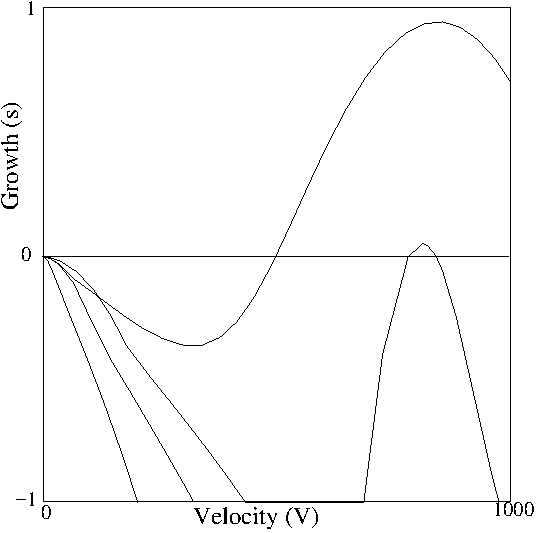
\includegraphics[height=8.0cm,width=8.0cm]{vso.pdf}
%% \centering
%% \caption{V-$\sigma$ at 100 rpm}\label{fig:whirl-vso}
%% \end{figure}
%% 
%% \begin{figure}[hbt!]
%% \includegraphics[height=8.0cm,width=8.0cm]{beta.pdf}
%% \centering
%% \caption{Variation of flutter speed with blade angle}\label{fig:beta}
%% \end{figure}


\newpage
\section{Atmospheric properties}\label{sect:atmos}
\Tableref{table:atmos} list properties of the standard atmosphere
from \cite{united1976us}.

\begin{table}[h]  % table:atmos
\begin{tabular}{|c|c|c|c|c|c|c|c|c|c|} \hline
{\bf Altitude } & {\bf Temperature}  & {\bf Pressure} & {\bf Density} & {\bf Sonic Velocity} \\
$Km$            & $\deg K$           & $Pa$ ($N/m^2$)        & $kg/m^3$      & $m/s$ \\ \hline
  -2 & 301.2 & 127800 & 1.478 & 347.9 \\ \hline
   0 & 288.150 & 101325 & 1.225 & 340.3 \\ \hline
   2 & 275.2 & 79500 & 1.007 & 332.5 \\ \hline
   4 & 262.2 & 61660 & 0.8193 & 324.6 \\ \hline
   6 & 249.2 & 47220 & 0.6601 & 316.5 \\ \hline
   8 & 236.2 & 35650 & 0.5258 & 308.1 \\ \hline
  10 & 223.3 & 26500 & 0.4.135 & 299.5 \\ \hline
  12 & 216.6 & 19400 & 0.3119 & 295.1 \\ \hline
  14 & 216.6 & 14170 & 0.2279 & 295.1 \\ \hline
  16 & 216.6 & 10350 & 0.1665 & 295.1 \\ \hline
  18 & 216.6 & 7565 & 0.1216 & 295.1 \\ \hline
  20 & 216.6 & 5529 & 0.08891 & 295.1 \\ \hline
  22 & 218.6 & 4048 & 0.06451 & 296.4 \\ \hline
  24 & 220.6 & 2972 & 0.04694 & 297.7 \\ \hline
  26 & 222.5 & 2188 & 0.03426 & 299.1 \\ \hline
  28 & 224.5 & 1616 & 0.02508 & 300.4 \\ \hline
  30 & 226.5 & 1197 & 0.01841 & 301.7 \\ \hline
  40 & 250.3 & 287.1 & 0.003996 & 317.2 \\ \hline
  50 & 270.6 & 79.78 & 0.001027 & 329.8 \\ \hline
  60 & 247.0 & 21.96 & 0.0003097 & 315.1 \\ \hline
  70 & 219.6 & 5.221 & 8.283(-5) & 297.1 \\ \hline
  80 & 198.6 & 1.052 & 1.846(-5) & 282.5 \\ \hline
\end{tabular}
\caption{Atmospheric properties} \label{table:atmos}
\index{atmospheric properties}
\index{altitude}
\index{density}
\index{temperature}
\index{pressure!static}
\index{static pressure}
\index{sonic velocity}
\end{table}

\newpage

\section{Substructuring for Flutter Analyses}\label{sect:ss-intro}
\index{substructuring}
Substructures are, as the name implies, pieces of a finite-element
model which are assembled to form the structure being modeled.
Depending on your point of view, the equivalent term
\Newterm{superelement} might be preferred:
a \Ss\ is a piece of a larger structure or
a superelement is a collection of finite-elements.
Here we use the terms interchangeably.

In dynamic analysis
\Sss\ are used to break a large structure into smaller pieces to:
\begin{itemize}
\item make the solution more economical by reducing the size of the model
	and allowing modifications to be carried out on only part of the model,
\item allow the design and analysis of a structure to be split
	among different groups
\end{itemize}
More important for flutter equations is isolating certain substructures to allow for:
% the elimination of stiffness coupling for certain degrees-of-freedom to facilitate
\begin{itemize}
\item stiffness parameter studies
\item nonlinearities with describing functions
\item control-systems
\end{itemize}
Isolating a substructure for these requirements means eliminating stiffness
coupling between it's dof and those of other substructures.

% In many cases these can be treated well with Branch Modes;
With these flutter requirements in mind we
give a brief summary of substructuring methods, starting with static
substructures, Guyan reduction, Branch Mode Analysis (BMA), and Component Mode
Synthesis (CMS).

Throughout this section substructures are partitioned into dof that attach
to other substructures, and all other dof, the interior dof. These are denoted
by subscripts a and i, respectively. Another subscript used is m, the number of
modal dof.

\subsection{\label{sect:static-ss}Static Substructuring}
\par
Static superelements are merged by creating a matrix of the correct size
and inserting the matrix elements in the appropriate spot with
overlapping elements accumulating.
For example if the mass and stiffness matrices for \Ss\ A have the form
\begin{equation}
\Matrix{A} = \left[
\begin{array}{cc}
   \Matrix{A}_{ii} & \Matrix{A}_{ia} \\
   \Matrix{A}_{ai} & \Matrix{A}_{aa}
\end{array}
\right]	\nonumber
\end{equation}
where the $i$ subscripts refer to interior dof and the $a$
subscripts refer to dof common with B, and \Ss\ B has
\begin{equation}
\Matrix{B} = \left[
\begin{array}{cc}
   \Matrix{B}_{aa} & \Matrix{B}_{ai} \\
   \Matrix{B}_{ia} & \Matrix{B}_{ii}
\end{array}
\right]	\nonumber
\end{equation}
The merged \Ss\ C will have
\begin{equation}\label{eqn:merged-ss}
\Matrix{C} = \left[
\begin{array}{ccc}
   \Matrix{A}_{ii} & \Matrix{A}_{ia} & \Matrix{0} \\
   \Matrix{A}_{ai} & \Matrix{A}_{aa} + \Matrix{B}_{aa} & \Matrix{B}_{ai} \\
   \Matrix{0} & \Matrix{B}_{ia} & \Matrix{B}_{ii}
\end{array}
\right]
\end{equation}
In general there is mass and stiffness coupling between the
interior and boundary dof of a static \Ss, hence
there is also mass and stiffness coupling between
merged \Sss.

\subsection{\label{sect:guyan-red}Guyan Reduction}
A common technique in static substructuring is to reduce the
model size with static condensation, where the equations of
static equilibrium are divided into dof to be eliminated and to be
retained; here we use static condensation to lump the interior stiffness 
to the attachment dof:
\begin{equation}
\Matrix{K} = \left[
\begin{array}{cc}
   \Matrix{K}_{aa} & \Matrix{K}_{ai} \\
   \Matrix{K}_{ia} & \Matrix{K}_{ii}
\end{array}
\right]
\left\{
\begin{array}{c}
   \Vector{x}_a \\
   \Vector{x}_i
\end{array}
\right\} =
\left\{
\begin{array}{c}
   \Vector{f}_a \\
   \Vector{f}_i
\end{array}
\right\}		\nonumber
\end{equation}
Assuming $\Vector{f}_i$ is negligible, these 2 equations result in
\begin{equation}\label{eqn:static-cond}
\left[\Matrix{K}_{aa}
	- \Matrix{K}_{ai}\Matrix{K}_{ii}^{-1}\Matrix{K}_{ia}\right]
		\Vector{x}_a = \Vector{f}_a
\end{equation}
and the condensed stiffness matrix
\begin{equation}\label{eqn:condensedK}
\Matrix{\bar{K}}_{aa} = 
	\Matrix{K}_{aa} - \Matrix{K}_{ai}\Matrix{K}_{ii}^{-1}\Matrix{K}_{ia}
\end{equation}
is equivalent to the transformation
$\Matrix{\bar{K}}_{aa} = \Matrix{G}_a^t\Matrix{K}\Matrix{G}_a$
where
\begin{equation} \label{eqn:static-ss}
\Matrix{G}_a = \left[
	\begin{array}{c}
		\Matrix{I}_a \\
		-\Matrix{K}_{ii}^{-1}\Matrix{K}_{ia}
	\end{array} \right] =
	\left[\begin{array}{c}
		\Matrix{I}_a \\
		\Matrix{G}_{ia}
	\end{array} \right]
\end{equation}
reduces to the $a$ dof, and $\Matrix{I}_a$ is the identity order $a$.

Guyan reduction \cite{guyan1965reduction}
applies this transformation to the mass matrix
\begin{equation}\label{eqn:guyanM}
\Matrix{\bar{M}}_{aa} = \Matrix{G}_a^t\Matrix{M}\Matrix{G}_a =
	\Matrix{M}_{aa} + \Matrix{M}_{ai}\Matrix{G}_{ia}
		+ \Matrix{G}_{ia}^t \Matrix{M}_{ia}
			+ \Matrix{G}_{ia}^t\Matrix{M}_{ii}\Matrix{G}_{ia}
\end{equation}
In the past Guyan reduction was used extensively prior to solving
the vibration eigenvalue problem; vibration modes were then used to
reduce the size of the flutter equation.
These days vibration problems are solved with sparse eigenvalue solvers,
so Guyan reduction, which destroys sparsity, is not used as much.
It is useful however in developing some substructuring techniques.

\subsection{Branch Mode Analysis}\label{sect:bma}\index{Branch Modes}\index{BMA}
\index{substructuring!Branch Mode Analysis}
Branch Mode Analysis (BMA) (\cite{gladwell1964branch}) is a modeling technique that
works well for structures with appendages, such as control surfaces,
wing-mounted engines, or landing gears.  An example shows how the method
works.

Aircraft often have engines mounted on the wings; call the wing
substructure A, or the \Newterm{root} substructure in BMA terminology,
and the engine substructure B, or the \Newterm{branch} substructure.
Two vibration solutions are performed: 1) the wing with the engine rigidly attached,
and 2) the engine cantilevered at the attachment to the wing. Merging these two
sets of modes and reducing the structure with it results in generalized mass and
stiffness matrices shown in \Figref{fig:bm-km}.  What is notable about this figure is
although there is mass coupling between the root and branch, there
is no stiffness coupling, satisfying the requirements in \Sectref{sect:ss-intro}.
% \begin{figure}
% 	\centering
% 	\includegraphics[height=9.0cm,width=5.0cm]{bma_phi.eps}
% 	\caption{Merged A and B BMA modes}\label{fig:bma-phi}
% \end{figure}

\begin{figure}
\centering
	\includegraphics[height=6cm,width=12cm]{bmodes.eps}
\caption{Example BMA reduced mass and stiffness}\label{fig:bm-km}
\end{figure}

\subsection{Component Mode Synthesis}\label{sect:cms}
\par
The terms Component Mode Synthesis (CMS) or \Newterm{Modal Synthesis}
\index{Modal Synthesis|see{CMS}} \index{substructuring!CMS}\index{CMS}
refer to a number of similar methods;
among these the method of Craig and Bampton \cite{craig1968coupling}
is probably the most straightforward and popular.
\par
Unlike BMA, CMS treats all substructures the same: all attachment dof
with other substructures are retained, while the interior dof are reduced using
vibration modes with the attachment supported. This leads to generalized mass
and stiffness matrices with the form shown in \Figref{fig:ss-cms}.
% In the Craig and Bampton approach when a \Ss\ is transformed to a dynamic \Ss\
% it retains the same nodal dof on the boundary, but the interior
% dof are replaced with generalized coordinates based on
% vibration modes computed with the boundary freedoms supported.
% Typical mass and stiffness matrices for a dynamic superelement
% retaining $m$ interior vibration modes
% are shown in figure \ref{fig:ss-cms}.
\begin{figure}
	\centering
	\includegraphics[height=4.0cm,width=9.0cm]{cms.eps}
	\caption{Merged A and B CMS mass and stiffness}\label{fig:ss-cms}
\end{figure}

Two characteristics of this method make it particularly attractive
for many structural-dynamics analyses:
\begin{itemize}
\item
{\bfseries They can be treated like static superelements\/}.
Because the attachment dof are left as nodal dof, the dynamic superelement
can be merged with other (static or dynamic) superelements
as though it were a static superelement.
% For example, if superelement A is a static superelement,
% while superelement B is a dynamic superelement, the
% merged mass and stiffness matrices will appear as in figure
% \ref{SUPEREL-F3}.
                
\item {\bfseries No stiffness coupling.} The other important
	characteristic of Craig and Bampton CMS is that there is no
	stiffness coupling between the interior dof and the attachment
	dof so when the \Ss\ is merged with other \Sss\ there is no
	stiffness coupling between the interior dof and other \Sss.
	Nor is there stiffness coupling between interior dof
	(the interior portion of the stiffness matrix is diagonal).
	This property makes it easy to do parameter studies of the
	influence of stiffness of a \Ss\ on, for example flutter speed.
\end{itemize}
Disadvantages to this method include
\begin{itemize}
\item Once a CMS structure is assembled the attachment dof are no longer
of interest and just add to the cost of a flutter analysis.
\item the vibration modes for the interior dof with the attachment dof
	supported are not as realistic for some structures as branch modes,
	as illustrated in the following example.
\end{itemize}

\subsection{Example: comparison of BMA and CMS modes}
An airplane wing with 2 propeller engines can be split into 3 substructures:
the wing, and the 2 engines. Calling the wing the root substructure and the engines
the branches, a BMA analysis gives the first 3 modes shown in \Figref{fig:bma-modes}.
\begin{figure}
	\centering
	\includegraphics[height=8.0cm,width=6.0cm]{bma_modes.eps}
	\caption{First 3 BMA modes}\label{fig:bma-modes}
\end{figure}
In contrast, a CMS reduction of the model gives the first 3 modes in \Figref{fig:cms-modes}.
\begin{figure}
	\centering
	\includegraphics[height=8.0cm,width=6.0cm]{cms_modes.eps}
	\caption{First 3 CMS modes}\label{fig:cms-modes}
\end{figure}
Clearly the BMA modes are more representative of the low-frequency modes of the
structure.

Figure \Figref{fig:ss-phi} compares the structure of BMA and CMS modes;
with the same numbers of modes from the interior vibration solutions the BMA 
modes are smaller due to the CMS constraint modes (ia).
\begin{figure}
	\centering
	\includegraphics[height=6.0cm,width=9.0cm]{ss_phi.eps}
	\caption{Merged A and B substructure modes}\label{fig:ss-phi}
\end{figure}

\subsection{Mathematical Details}
\subsubsection{BMA}
% Using Guyan reduction, the engine mass is reduced to the nodal interface
% between A and B, and a vibration solution gives the modes of the wing as if
% the engine were rigidly attached. If the interace is statically determinant,
% for example if it consists of only one node, adding the rigid motion of
% the engine to these modes is straightforward. Next, a vibration solution of the engine
% cantilevered at the interface

% that can be divided into substructures with
% simple interfaces. For example, control surfaces on aircraft can often
% be modeled as a rigid substructure with a rotational degree-of-freedom
% about the hinge line. This allows a straightforward addition of a
% control system, studies of the effect of actuator stiffness on flutter,
% and the approximation of nonlinearities due to hinge freeplay.
% Similarly, modeling propellers on propeller-driven aircraft, and
% wing-mounted engines on jet aircraft with branch modes has
% these same advantages.

%% The key to the success of Branch Modes is in the form of the mass and
%% stiffness matrices: there is mass coupling but no stiffness coupling
%% between substructures.
% takes it's name from the type of structure it is most suited for:
% a small beam attached
% to a larger beam.  Examples from aircraft include control surfaces,
% jet engines, propellers, and landing gears, where it has proven to
% be an expedient way to do parameter studies and nonlinear analyses.
% Because it only applies to beam models it has fallen out of use
% in favor of finite-element models. Nevertheless it is worth reviewing
% with the goal of extending it to finite-element models in mind.

Conceptually branch-modes is simple: with one \Ss\ as the
root, and the other the branch, two free-vibration eigenvalue problems
are solved:
\begin{enumerate}
	\item the root \Ss\ (A) with the branch (B) rigidly attached using a
		Guyan transformation ($\Matrix{G}_a$) to the attachment
		\begin{eqnarray}
			\Matrix{K}^A\Matrix{\Phi}_m & = & \Matrix{\Lambda}^A\Matrix{M}^{A+}\Matrix{\Phi}_m \\
			\Matrix{M}^{A+} &=& \left[\begin{array}{cc}
				\Matrix{M}^A_{ii}  &  \Matrix{M}^A_{ia} \nonumber \\
				\Matrix{M}^A_{ai}  &  \Matrix{M}^A_{aa} + \Matrix{G}^t_a\Matrix{M}^B\Matrix{G}_a
			\end{array}\right]
		\end{eqnarray}
		for $m$ eigenvectors
		\begin{equation}
			\Matrix{\Phi}_m = \left\{\begin{array}{c}
				\Matrix{\Phi}_{im}	\nonumber \\
				\Matrix{\Phi}_{am}	\nonumber
			\end{array}\right\}
		\end{equation}
		and the motion of the interior of B due to the attachment:
		\begin{equation}
			\Matrix{\Phi}_{jm} = \Matrix{G}_{ja}\Matrix{\Phi}_{am}	\nonumber
		\end{equation}
	\item the branch \Ss\ (B) clamped at the attachment
	\begin{equation}
		\Matrix{K}^B_{jj}\Matrix{\Phi}_{jp} = \Matrix{\Lambda}^B\Matrix{M}^B_{jj}\Matrix{\Phi}_{jp}
	\end{equation}
	for $p$ eigenvectors $\Matrix{\Phi}_{jp}$.
\end{enumerate}
The 2 sets of eigenvectors are combined to form a transformation
matrix
\begin{equation}\label{eqn:bmt}
\Matrix{\Phi} = \left[
	\begin{array}{cc}
		\Matrix{\Phi}_{im} & \Matrix{0} \\
		\Matrix{\Phi}_{bm} & \Matrix{0} \\
		\Matrix{\Phi}_{jm} & \Matrix{\Phi}_{jp}
	\end{array} \right]
\end{equation}
\index{=Phi@$\Matrix{\Phi}$!branch modes}
% where the $i$ subscript refers to the interior dof of the root,
% $j$ the interior of the branch, $b$ the boundary between them,
% $m$ and $p$ the number of modes retained in the root ($\Phi$) and
% branch ($\Phi$) eigenvectors, respectively.
Applying this transformation to the static-merged mass and stiffness
matrices gives the branch-mode mass and stiffness:
\begin{equation}
	\Matrix{\bar{M}} = \Matrix{\Phi}^t \Matrix{M} \Matrix{\Phi},\hspace{0.5cm}
	\Matrix{\bar{K}} = \Matrix{\Phi}^t \Matrix{K} \Matrix{\Phi},
\end{equation}
illustrated in \Figref{fig:bm-km}. What is notable about this figure is
although there is mass coupling between the root and branch, there
is no stiffness coupling.
% To show why this is so, consider 2 equivalent partitionings of $\Matrix{\Phi}$,
% \begin{eqnarray}
% \Matrix{\Phi}_1 &=& \left[
% 	\begin{array}{cc}
% 		\Matrix{\Phi}_{m} & \Matrix{0} \\
% 		\Matrix{\Phi}_{jm} & \Matrix{\Phi}_{jp}
% 	\end{array} \right], \hspace{0.5cm}
% 		\Matrix{\Phi}_m = \left[\begin{array}{c}
% 			\Matrix{\Phi}_{im} \\
% 			\Matrix{\Phi}_{bm}
% 		\end{array}\right] \nonumber \\
% \Matrix{\Phi}_2 &=& \left[
% 	\begin{array}{cc}
% 		\Matrix{\Phi}_{im} & \Matrix{0} \\
% 		\Matrix{\Phi}_{r} & \Matrix{\Phi}_{jp}
% 	\end{array} \right], \hspace{0.5cm}
% 		\Matrix{\Phi}_r = \left[\begin{array}{c}
% 			\Matrix{\Phi}_{bm} \\
% 			\Matrix{\Phi}_{jm}
% 		\end{array}\right]
% \end{eqnarray}
% where $\Matrix{\Phi}_m$ are the eigenvectors from problem (1) and
% $\Matrix{\Phi}_r$ is the rigid motion of the branch in problem (1).
% Similarly, partition $\Matrix{K}$
% \begin{equation}
% \Matrix{K} = \left[\begin{array}{cc}
% 	\Matrix{K}^A & \Matrix{0} \\
% 		\Matrix{0} & \Matrix{0}
% 	\end{array} \right] +
% 	\left[\begin{array}{cc}
% 	\Matrix{0} & \Matrix{0} \\
% 		\Matrix{0} & \Matrix{K}^B
% 	\end{array} \right]
% \end{equation}
% and since $\Matrix{K}^B\Matrix{\Phi}_r = 0$
% \begin{eqnarray}
% \Matrix{\bar{K}} &=&
% 	\Matrix{\Phi}_1^t \left[\begin{array}{cc}
% 		\Matrix{K}^A & \Matrix{0} \\
% 			\Matrix{0} & \Matrix{0}
% 		\end{array} \right] \Matrix{\Phi}_1 +
% 		\Matrix{\Phi}_2^t \left[\begin{array}{cc}
% 			\Matrix{0} & \Matrix{0} \\
% 			\Matrix{0} & \Matrix{K}^B
% 		\end{array} \right] \Matrix{\Phi}_2 \nonumber \\
% 	&=& 
% 	\left[\begin{array}{cc}
% 		\Matrix{\Phi}_m^t\Matrix{K}^A\Matrix{\Phi}_m & \Matrix{0} \\
% 		\Matrix{0} & \Matrix{0}
% 	\end{array} \right] +
% 		\left[\begin{array}{cc}
% 			\Matrix{0} & \Matrix{0} \\
% 			\Matrix{0} & \Matrix{\Phi}_{jp}^t{K}_{jj}^B\Matrix{\Phi}_{jp}
% 		\end{array} \right] \Matrix{\Phi}_2
% \end{eqnarray}
% Likewise,
% \begin{eqnarray}
% \Matrix{\bar{M}} &=&
% 	\Matrix{\Phi}_1^t \left[\begin{array}{cc}
% 		\Matrix{M}^A & \Matrix{0} \\
% 			\Matrix{0} & \Matrix{0}
% 		\end{array} \right] \Matrix{\Phi}_1 +
% 		\Matrix{\Phi}_2^t \left[\begin{array}{cc}
% 			\Matrix{0} & \Matrix{0} \\
% 			\Matrix{0} & \Matrix{M}^B
% 		\end{array} \right] \Matrix{\Phi}_2 \nonumber \\
% 	&=& 
% 	\left[\begin{array}{cc}
% 		\Matrix{\Phi}_m^t\Matrix{M}^A\Matrix{\Phi}_m & \Matrix{0} \\
% 		\Matrix{0} & \Matrix{0}
% 	\end{array} \right] \nonumber \\
% 	&+& \left[\begin{array}{cc}
% 			\Matrix{\Phi}_r\Matrix{M}^B\Matrix{\Phi}_r & \text{symmetric} \\
% 			\Matrix{\Phi}_{jp}^t\Matrix{M}_{jb}^B\Matrix{\Phi}_{bm}
% 			+ \Matrix{\Phi}_{jp}^t\Matrix{M}_{jj}^B\Matrix{\Phi}_{jm} & \Matrix{\Phi}_{jp}^t\Matrix{M}_{jj}^B\Matrix{\Phi}_{jp}
% 		\end{array} \right]
% \end{eqnarray}
% which shows the mass coupling term
% $\Matrix{\Phi}_{jp}^t\Matrix{M}_{jb}^B\Matrix{\Phi}_{bm} + \Matrix{\Phi}_{jp}^t\Matrix{M}_{jj}^B\Matrix{\Phi}_{jm}$, and the diagonal blocks are diagonal due to
% the 2 free-vibration problems.
% What is notable about this figure is although there is mass coupling
% between the root and branch, there is no stiffness coupling; that,
% and the fact that the branch dof are now based on cantilevered modes,
% makes stiffness variations, freeplay analysis, and correlation with
% vibration tests very easy.
\subsubsection{CMS}
\par
A CMS substructure is formed from an (n,n) static \Ss\
by the coordinate transformation

\begin{equation}\label{eqn:dsstrans}
\begin{split}
\Matrix{\bar{K}} & \, = \, \Matrix{\Phi}^T \Matrix{K} \Matrix{\Phi} \\
\Matrix{\bar{M}} & \, = \, \Matrix{\Phi}^T \Matrix{M} \Matrix{\Phi}
\end{split}
\end{equation}
where $\Matrix{\Phi}$ is the $(n,n_k )$ CMS modes matrix,
$\Matrix{M}$ and $\Matrix{K}$
are the $(n,n)$ static substructure mass and stiffness matrices, and
$\Matrix{\bar{M}}$ and $\Matrix{\bar{K}}$ are the $(n_k , n_k)$
CMS generalized mass and stiffness matrices.
The CMS modes matrix consists of free-vibration
modes with the attachment freedoms supported and so-called
\Newterm{constraint modes}.
Constraint modes are the displacement pattern resulting
from  giving each attachment freedom in turn a unit displacement while
the remaining attachment freedoms are fixed.
Mathematically this is equivalent to solving the linear equations

\begin{equation}\label{eqn:dsslineqn}
\Matrix{K}\Matrix{\Phi}_a = \left[
\begin{array}{cc}
   \Matrix{K}_{aa} & \Matrix{K}_{ai} \\
   \Matrix{K}_{ia} & \Matrix{K}_{ii}
\end{array}
\right] \left[
\begin{array}{c}
   \Matrix{I}_{aa} \\
   \Matrix{\Phi}_{ia}
\end{array}
\right] = \left[
\begin{array}{c}
   \Matrix{F}_{aa} \\
   \Matrix{0}_{ia}
\end{array}
\right]
\end{equation}
\index{=Phi@$\Matrix{\Phi}$!modal synthesis}
where $\Matrix{F}_{aa}$ are the forces necessary to produce the unit
displacements. These forces are of no interest so we simply need to solve
for the constraint modes
\begin{equation}\label{eqn:constraint}
	\left[ \begin{array}{c}
		\Matrix{I}_{aa} \\
		\Matrix{\Phi}_{ia}
	\end{array} \right] =
	\left[ \begin{array}{c}
		\Matrix{I}_{aa} \\
		-\Matrix{K}_{ii}^{-1} \Matrix{K}_{ia}
	\end{array} \right]
\end{equation}
which is the static condensation (\Eqn{eqn:static-ss}) of the interior to the attachment.

Free-vibration modes are computed using the interior
partitions of the mass and stiffness matrices:
\begin{equation}\label{eqn:cms-eig}
\Matrix{K}_{ii} \Matrix{\Phi}_{im} = \Matrix{M}_{ii} \Matrix{\Phi}_{im} \Matrix{\Lambda}_{mm}
\end{equation}
where $\Matrix{\Lambda}_{mm}$ is an $(m,m)$ diagonal matrix
of eigenvalues, and the number of computed modes $0 \leq m \leq i$.
The $m$ computed modes are a basis for the generalized
coordinates representing the interior degrees-of-freedom.

The assembled CMS transformation matrix is
\begin{equation}
\Matrix{\Phi} = \left[
\begin{array}{cc}
   \Matrix{\Phi}_{im} & \Matrix{\Phi}_{ia} \\
   \Matrix{0} & \Matrix{I}_{aa}
\end{array}
\right]			\nonumber
\end{equation}
Substituting \Eqn{eqn:dsslineqn} and \Eqn{eqn:cms-eig} into \Eqn{eqn:dsstrans}:
\begin{equation}
\begin{split}
\Matrix{\bar{K}} & \, = \, \left[
        \begin{array}{cc}
                \Matrix{\Phi}_{mk} & \Matrix{\Phi}_{ia} \\
                \Matrix{0} & \Matrix{I}_{aa}
        \end{array}
        \right]^T \left[
        \begin{array}{cc}
                \Matrix{K}_{ii} & \Matrix{K}_{ia} \\
                \Matrix{K}_{ai} & \Matrix{K}_{aa}
        \end{array}
        \right]^T \left[
        \begin{array}{cc}
                \Matrix{\Phi}_{im} & \Matrix{\Phi}_{ia} \\
                \Matrix{0} & \Matrix{I}_{aa}
        \end{array}
        \right]                                 \\
 & \, = \, \left[
\begin{array}{cc}
   \Matrix{\Phi}_{im}^T \Matrix{K}_{ii} \Matrix{\Phi}_{im} & symmetric \\
   \Matrix{\Phi}_{ia}^T \Matrix{K}_{ii} \Matrix{\Phi}_{im} + \Matrix{K}_{ai} \Matrix{\Phi}_{im} &
                        \Matrix{\Phi}_{ia}^T \Matrix{K}_{ii} \Matrix{\Phi}_{ia} +
                        \Matrix{K}_{ai} \Matrix{\Phi}_{ia} + \Matrix{\Phi}_{ia}^T \Matrix{K}_{ia} + \Matrix{K}_{aa}
\end{array}
\right]
\end{split}		\nonumber
\end{equation}
Using the fact that $\Matrix{K}_{ai} = \Matrix{K}_{ia}^T$ (symmetry)
and the definition of constraint modes (\Eqn{eqn:constraint})
\begin{equation}
\Matrix{\Phi}_{ia}^T \Matrix{K}_{ii} \Matrix{\Phi}_{im} + \Matrix{K}_{ai} \Matrix{\Phi}_{im} =
                \left( \Matrix{K}_{ii} \Matrix{\Phi}_{ia} + \Matrix{K}_{ia} \right)^T \Matrix{\Phi}_{im} = \Matrix{0}		\nonumber
\end{equation}
shows that there is no coupling between interior and boundary freedoms.

Again using the definition of constraint modes,
\begin{equation}
\Matrix{\Phi}_{ia}^T \Matrix{K}_{ii} \Matrix{\Phi}_{ia} =
                - \Matrix{K}_{ai} \Matrix{\Phi}_{ia} = - \Matrix{\Phi}_{ia}^T \Matrix{K}_{ia}		\nonumber
\end{equation}
and
\begin{equation}
\Matrix{\bar{K}}_{kk} = \Matrix{\Phi}_{im} \Matrix{K}_{ii} \Matrix{\Phi}_{im}	\nonumber
\end{equation}
is diagonal due to \Eqn{eqn:cms-eig}.
Using these relations the generalized stiffness matrix $\Matrix{\bar{K}}$
can be written as
\begin{equation}
\begin{split}
\Matrix{\bar{K}} & \, = \, \left[
\begin{array}{cc}
   \Matrix{\bar{K}}_{kk} & \Matrix{0} \\
   \Matrix{0} & \Matrix{K}_{aa} + \frac{1}{2} \left( \Matrix{K}_{ia}^T \Matrix{\Phi}_{ia} + \Matrix{\Phi}_{ia}^T \Matrix{K}_{ia} \right)
\end{array}
\right]         \\
 & \, = \, \left[
\begin{array}{cc}
   \Matrix{\bar{K}}_{kk} & \Matrix{0} \\
   \Matrix{0} & \Matrix{K}_{aa} - \Matrix{\Phi}_{ia}^T \Matrix{K}_{ii}^T \Matrix{\Phi}_{ia}
\end{array}
\right]         \\
 & \, = \, \left[
\begin{array}{cc}
   \Matrix{\bar{K}}_{kk} & \Matrix{0} \\
   \Matrix{0} & \Matrix{K}_{aa} - \Matrix{K}_{ia}^T \Matrix{K}_{ii}^{-1} \Matrix{K}_{ia}
\end{array}
\right]
\end{split}			\nonumber
\end{equation}
In the last of these three alternative forms the block
$\Matrix{K}_{aa} - \Matrix{K}_{ia}^T \Matrix{K}_{ii}^{-1} \Matrix{K}_{ia}$
is recognized as the static condensation (\Eqn{eqn:condensedK}) of
the \Ss\ stiffness matrix to the boundary dof. The generalized
mass matrix,
\begin{equation}
\begin{split}
\Matrix{\bar{M}} & \, = \\
 &  \left[
\begin{array}{cc}
   \Matrix{\Phi}_{im}^T \Matrix{M}_{ii} \Matrix{\Phi}_{im} & symmetric \\
   \Matrix{\Phi}_{ia}^T \Matrix{M}_{ii} \Matrix{\Phi}_{im} + \Matrix{M}_{ai} \Matrix{\Phi}_{im} &
                        \Matrix{\Phi}_{ia}^T \Matrix{M}_{ii} \Matrix{\Phi}_{ia} +
                        \Matrix{M}_{ai} \Matrix{\Phi}_{ia} + \Matrix{\Phi}_{ia}^T \Matrix{M}_{ia}
                                + \Matrix{M}_{aa}
\end{array}
\right]
\end{split}		\nonumber
\end{equation}
shows that there is, in general, mass coupling between the
boundary and interior generalized coordinates.
The lower-right block is recognized as the Guyan reduction
\index{Guyan reduction!in CMS}
(\Eqn{eqn:guyanM})
of the mass matrix to the boundary dof.

Because the boundary partitions of the CMS mass and stiffness
are Guyan reductions of the interior to the boundary, rigid-body
motion only affects the boundary partitions. This can be shown
by applying
the coordinate transformation to an arbitrary vector
\begin{equation}
\Vector{\bar{v}} = \left[
\begin{array}{c}
\Vector{\bar{v}}_k \\
\Vector{\bar{v}}_a
\end{array}
\right]				\nonumber
\end{equation}
where here again the $k$
subscript refers to the ``kept'' cantilevered vibration modes and the
$a$ refers to the attachment dof, the resulting vector $\Vector{v}$ is
\begin{equation}
\Vector{v} = \left[
\begin{array}{c}
\Vector{v}_i \\
\Vector{v}_a
\end{array}
\right] = \Matrix{\Phi} \Vector{\bar{v}} = \left[
\begin{array}{cc}
\Matrix{\Phi}_{im} & \Matrix{\Phi}_{ia} \\
\Matrix{0} & \Matrix{I}_{aa}
\end{array}
\right] \left[
\begin{array}{c}
\Matrix{\bar{v}}_k \\
\Matrix{\bar{v}}_a
\end{array}
\right] = \left[
\begin{array}{c}
\Matrix{\Phi}_{im} \Vector{\bar{v}}_k + \Matrix{\Phi}_{ia} \Vector{\bar{v}}_a \\
\Vector{\bar{v}}_{a}
\end{array}
\right]			\nonumber
\end{equation}
which shows that the boundary coordinates are not affected by the
transformation. In particular if $\Matrix{r}$ is a rigid-body vector
for the static substructure, then
\begin{equation}
\Vector{\bar{r}} = \left\{
        \begin{array}{c}
                \Vector{0}                \\
                \Vector{r}_{a}
        \end{array}
\right\}					\nonumber
\end{equation}
is a rigid-body vector for the CMS substructure, because
\begin{equation}
\begin{split}
\Matrix{K}\Vector{r} & \, = \, \left[
\begin{array}{cc}
   \Matrix{K}_{ii} & \Matrix{K}_{ia} \\
   \Matrix{K}_{ai} & \Matrix{K}_{aa}
\end{array}
\right] \left\{
\begin{array}{c}
   \Matrix{\Phi}_{ia} \Matrix{r}_a \\
   \Matrix{r}_a
\end{array}
\right\} =  \left\{
\begin{array}{c}
   \Matrix{K}_{ii} \Matrix{\Phi}_{ia} \Matrix{r}_a + \Matrix{K}_{ia} \Matrix{r}_a \\
   \Matrix{K}_{ai} \Matrix{\Phi}_{ia} \Matrix{r}_a + \Matrix{K}_{aa} \Matrix{r}_a
\end{array}
\right\}                                        \\
 & = \, \left\{
\begin{array}{c}
   - \Matrix{K}_{ia} \Vector{r}_a + \Matrix{K}_{ia} \Vector{r}_a \\
   - \Matrix{\Phi}_{ia}^T \Matrix{K}_{ii} \Matrix{\Phi}_{ia}^T \Vector{r}_a +
                \Matrix{K}_{aa} \Vector{r}_a
\end{array}
\right\} \\
 & = \, \left\{
\begin{array}{c}
   \Matrix{0} \\
   \Matrix{K}_{aa} \Vector{r}_a -
                        \Matrix{\Phi}_{ia}^T \Matrix{K}_{ii} \Matrix{\Phi}_{ia} \Vector{r}_a
\end{array}
\right\} = \Vector{0}
\end{split}		\nonumber
\end{equation}
by definition, so that
\begin{equation}
\Matrix{\bar{K}} \Matrix{\bar{r}} = \left\{
\begin{array}{c}
   \Vector{0} \\
   \Matrix{K}_{aa} \Vector{r}_a - \Matrix{\Phi}_{ia}^T \Matrix{K}_{ii} \Matrix{\Phi}_{ia} \Vector{r}_a
\end{array}
\right\} = \Vector{0}		\nonumber
\end{equation}
also. Rigid body motion is therefore only a function of the
boundary dof. This fact also follows from the fact
that the boundary portions of the generalized mass and
stiffness matrices are Guyan-reductions of the
interior freedoms.

\subsection{Branch Modes for FEM} \label{bm-extended}
As noted earlier
the branch modes procedure is straightforward
when applied to substructured models with statically-determinate
interfaces;
with a statically-indeterminate interface it is
not clear how to constrain superelement B to move rigidly
with A without constraining the boundary freedoms relative to one another.
This is where the use of a dynamic superelement reduction
of B can be used to advantage, since the motions of the
interior freedoms and boundary freedoms are separated
in a natural way.
Instead of constraining the interior freedoms to
move rigidly relative to the boundary freedoms,
we simply support (remove from the vibration analysis)
the generalized coordinates which represent the motion
of the interior freedoms.
This is {\bfseries almost\/}
the same as constraining the interior freedoms to
move rigidly relative to the boundary freedoms:
more precisely, it corresponds to Guyan-reducing
B to the boundary freedoms between A and B.
Motion of the boundary freedoms will result in
non-rigid motion of the interior freedoms of B according to
the definition of constraint modes (\Eqn{eqn:constraint}).
This type of motion is exactly what we want to prevent
unnatural constraints on the vibration modes of A.
\par
If the merged mass and stiffness matrices are reduced to
generalized coordinates based on the vibration modes of
the merged structure the branch mode property is lost.
What is needed is a generalized-coordinate transformation
based on modes which are capable of representing the true vibration
characteristics of the structure while retaining the branch mode
property.
In this section we show how to reduce the merged static and
dynamic superelement matrices to generalized coordinates
while retaining the branch mode nature of the stiffness matrix.
\subsubsection{Mathematical Details}
\par
Given 2 \Sss\ A and B (either or both may be dynamic \Sss)

\begin{equation}
\Matrix{K} = \left[
\begin{array}{ccc}
   \Matrix{K}_{ii}^A & \Matrix{K}_{ib}^A & \Matrix{0} \\
   \Matrix{K}_{bi}^A & \Matrix{K}_{bb}^A + \Matrix{\bar{K}}_{bb}^B & \Matrix{0} \\
   \Matrix{0} & \Matrix{0} & \Matrix{\bar{K}}_{kk}^B
\end{array}
\right]				\nonumber
\end{equation}


\begin{equation}
\Matrix{M} = \left[
\begin{array}{ccc}
   \Matrix{M}_{ii}^A & \Matrix{M}_{ib}^A & \Matrix{0} \\
   \Matrix{M}_{bi}^A & \Matrix{M}_{bb}^A + \Matrix{\bar{M}}_{bb}^B & \Matrix{\bar{M}}_{bi}^B \\
   \Matrix{0} & \Matrix{\bar{M}}_{ib}^B & \Matrix{\bar{M}}_{kk}^B
\end{array}
\right]			\nonumber
\end{equation}

The vibration problem for superelement A with rigid B amounts
to solving

\begin{equation}\label{eqn:femdynss}
\left( \Matrix{K}_{nn}^{A+} - \omega^2 \Matrix{M}_{nn}^{A+} \right)  \Matrix{\phi} = \Matrix{0}
\end{equation}
where the subscript $n$ represents all freedoms in A (i and b)
and the + superscript refers to the additional mass and stiffness
terms from B on the boundary,
\begin{equation}
\Matrix{K}_{nn}^{A+} = \left[
\begin{array}{cc}
   \Matrix{K}_{ii}^A & \Matrix{K}_{ib}^A  \\
   \Matrix{K}_{bi}^A & \Matrix{K}_{bb}^A + \Matrix{\bar{K}}_{bb}^B \\
\end{array}
\right]				\nonumber
\end{equation}
and
\begin{equation}
\Matrix{M}_{nn}^{A+} = \left[
\begin{array}{cc}
   \Matrix{M}_{ii}^A & \Matrix{M}_{ib}^A  \\
   \Matrix{M}_{bi}^A & \Matrix{M}_{bb}^A + \Matrix{\bar{M}}_{bb}^B \\
\end{array}
\right]
\end{equation}
That is, solve the vibration problem for superelement A
with superelement B Guyan-reduced to the A-B boundary and
added to the mass and stiffness matrices for A.
If B is a dynamic superelement the boundary mass and stiffness
terms \emph{are} Guyan reductions of B.

Solving \Eqn{eqn:femdynss} for m modes

\begin{equation}
\Matrix{\Phi}_{nm}^{A+} = \left[
\begin{array}{c}
   \Matrix{\Phi}_{im} \\
   \Matrix{\Phi}_{bm}  \\
\end{array}
\right]
\end{equation}


Reduced to this basis, the generalized mass and stiffness for A are

\begin{equation}
\begin{split}
\Matrix{\bar{M}}_{mm}^{A+} \, & = \,
        \left( \Matrix{\Phi}_{nm}^{A+} \right)^T
                \Matrix{M}_{nn}^{A+} \Matrix{\Phi}_{nm}^{A+} \\
        & \, = \, \Matrix{\Phi}_{im}^T \Matrix{M}_{ii}^A \Matrix{\Phi}_{im}
                + \Matrix{\Phi}_{im}^T \Matrix{M}_{ib}^A \Matrix{\Phi}_{bm} \\
         & \mbox{\hspace{0.2in}} +
                        \Matrix{\Phi}_{bm}^T \Matrix{M}_{bi}^A \Matrix{\Phi}_{im} +
                        \Matrix{\Phi}_{bm}^T \left(\Matrix{M}_{bb}^A +
                        \Matrix{M}_{bb}^B \right) \Matrix{\Phi}_{bm}
\end{split}
\end{equation}


and

\begin{equation}
\begin{split}
\Matrix{\bar{K}}_{mm}^{A+} \, & = \,
                        \left( \Matrix{\Phi}_{nm}^{A+} \right)^T
                        \Matrix{K}_{nn}^{A+} \Matrix{\Phi}_{nm}^{A+} \\
        & \, = \, \Matrix{\Phi}_{im}^T \Matrix{K}_{ii}^A \Matrix{\Phi}_{im} +
                        \Matrix{\Phi}_{im}^T \Matrix{K}_{ib}^A \Matrix{\Phi}_{bm} \\
        & \mbox{\hspace{0.2in}} +
                \Matrix{\Phi}_{bm}^T \Matrix{K}_{bi}^A \Matrix{\Phi}_{im} +
                \Matrix{\Phi}_{bm}^T \left(\Matrix{K}_{bb}^A +
                \Matrix{K}_{bb}^B \right) \Matrix{\Phi}_{bm}
\end{split}
\end{equation}


Now consider the transformation matrix
\begin{equation}
\Matrix{\Phi} = \left[
\begin{array}{cc}
   \Matrix{\Phi}_{nm}^{A+} & \Matrix{0} \\
   \Matrix{0} & \Matrix{I}_{kk}
\end{array}
\right] = \left[
\begin{array}{cc}
   \Matrix{\Phi}_{im} & \Matrix{0} \\
   \Matrix{\Phi}_{bm} & \Matrix{0} \\
   \Matrix{0} & \Matrix{I}_{kk}
\end{array}
\right]				\nonumber
\end{equation}
which when used to reduce the merged superelement matrices results in
\begin{equation}
\Matrix{\bar{K}} = \Matrix{\Phi}^T \Matrix{K} \Matrix{\Phi} = \left[
\begin{array}{cc}
   \Matrix{\bar{K}}_{mm}^{A+} & \Matrix{0} \\
   \Matrix{0} & \Matrix{\bar{K}}_{kk}^B
\end{array}
\right]			\nonumber
\end{equation}
and
\begin{displaymath}
\Matrix{\bar{M}} = \Matrix{\Phi}^T \Matrix{M} \Matrix{\Phi} = \left[
\begin{array}{cc}
   \Matrix{\bar{M}}_{mm}^{A+} & \Matrix{\bar{M}}_{mk} \\
   \Matrix{\bar{M}}_{km} & \Matrix{\bar{M}}_{kk}^B
\end{array}
\right]
\end{displaymath}
where the mass coupling term
\begin{displaymath}
\Matrix{\bar{M}}_{km} = \Matrix{\bar{M}}_{mk}^T = \Matrix{M}_{kb}^B \Matrix{\Phi}_{bm}
\end{displaymath}

$\Matrix{\bar{K}}$ and $\Matrix{\bar{M}}$ represent the entire structure
(A and B) in a modal basis with the following characteristics:
\begin{itemize}
\item $\Matrix{\bar{M}}_{kk}^B$ and $\Matrix{\bar{M}}_{mm}^{A+}$ are diagonal but
		$\Matrix{\bar{M}}$ is not, due to the mass coupling term $\Matrix{\bar{M}}_{km}$
\item $\Matrix{\bar{K}}$ is diagonal
\item the last $k$ generalized-coordinates are based on clamped vibration modes of B
\end{itemize}

The last two characteristics mean the branch mode property has been retained.
Figure \ref{fig:bm-km} illustrates the form of the generalized mass and stiffness.

\subsection{ Example: Strut Frequency Variations}
\par
Flutter modes of an airplane are often sensitive
to the fundamental frequencies of the strut/engine/nacelle,
so flutter groups study the variation of
flutter speed with strut frequencies.
These variations have in the past been simplified
by using the Branch Mode technique.
While Branch Modes will not work with finite element models,
the technique described above
provides an analogous technique.
\par
There are significant advantages to importing
the strut/engine/nacelle from \Nastran as a
dynamic superelement:

\begin{itemize}
\item
the correct loadpaths are maintained between
the wing and strut
\item
the dynamics of the strut/engine/nacelle can be
represented to any desired accuracy
by increasing the number of interior generalized
coordinates.
\item
much less data needs to be transmitted between groups;
a 30000 dof finite-element engine model could be represented
with a dynamic superelement with less than a hundred dof
with more accuracy than current beam representations.
\item
strut frequency parameter variations can be easily and
accurately performed
\end{itemize}


\section{Automatic Differentiation}\label{sect:AD}
\index{automatic differentiation|textbf}
A common task in scientific computing is to compute
derivatives of a function. Traditional methods for doing this
are writing custom software, numerical differentiation and symbolic differentiation.
Each have significant disadvantages: custom coding can be tedious
and error-prone; numerical differentiation
is prone to truncation and roundoff errors and can be expensive;
symbolic differentiation requires special software to preprocess
the function, such as Mathematica or Maple, and requires extra
effort by the user to learn and use the software.
A fourth alternative, automatic differentiation (AD)
\cite{rall1981automatic,autodiff}
is a programming technique that propagates derivatives
along with the evaluation of the function. It combines the advantages
of the other techniques: it is not much more expensive than
a simple evaluation of the function, does not require explicit coding
of derivatives, yet it yields exact derivatives.
The disadvantage is it requires a special library, either one of
the many freely available \cite{autodiff}, or writing your own.
\Flaps has it's own AD library tailored to the special requirements
of flutter analysis.
\par

\subsection{Implementation}
\Cpp allows you to create your own datatype, called
\Newterm{abstract datatypes}, and arithmetic operators and
functions to operate on them.
For purposes of illustration we define a
datatype we'll call \Code{Ad}\index{Ad@\Code{Ad} datatype}
which will take the place
of real variables. This new datatype has, in addition to
a real value, a derivative. That is, each variable of this 
type has allocated two real values in memory: the value and
the derivative which we denote here by adding a
\Code{value} and \Code{deriv} extension to the
variable name; for example
\begin{lstlisting}
   Ad a
   a.value = 1.0
   a.deriv = 2.0
\end{lstlisting}

declares that variable \Code{a} has a value of 1 and
it's derivative is 2.
\par
The other feature of modern programming
languages that make automatic differentiation possible is
known as \Newterm{operator overloading}. An overloaded
operator like multiplication allows you to write
\begin{lstlisting}
   c = a*b
\end{lstlisting}

where a, b, and c are variables of type \Code{Ad}.
The implementor of an automatic differentiation system,
following the rules of differentiation,
provides instructions to the compiler to translate this statement into
\begin{lstlisting}
   c.value = a.value*b.value
   c.deriv = a.deriv*b.value + a.value*b.deriv
\end{lstlisting}

Likewise for all the other arithmetic operators $(+-/)$.
Mathematical functions such as exponentials are handled similarly,
with overloaded functions\index{overloaded functions}, which have the same names
as the ordinary math functions, but are called by the compiler
when the argument is type \Code{Ad}.
For example
\begin{lstlisting}
   Ad exp(Ad a) {
      b.value = exp(a.value)
      b.deriv = a.value*a.deriv*exp(a.value)
      return b
   }
\end{lstlisting}

This and other overloaded math functions are also supplied
by the implementor.
\par
Now a programmer could use this automatic differentiation implementation
to write programs; for example
\begin{lstlisting}
   main() {
      Ad s;
      s.value = 10.0;
      s.deriv = 1.0;
      a = myfunc(s);
      cout << "a = " << a.value << endl;
      cout << "derivative of a wrt s = " << a.deriv << endl;
   }

   Ad myfunc(Ad s) {
      return sqrt(3.0*s + s*s + s*s*s);
   }
\end{lstlisting}
In this (stylized) program, s is the independent variable, so
it's derivative is always 1.0. Compiling and running this little program yields
\begin{lstlisting}
    a = 2.23607
    derivative of a wrt s = 1.78885
\end{lstlisting}
The only change to normal coding practice is the use of the
\Code{Ad} datatype in place of an floating-point datatype.

\subsection{\Flaps Implementation}
Derivatives are important in \Flaps, in particular for maintaining
continuity when tracking aeroelastic modes in \Cmd{flut}.
Automatic differentiation is used extensively in \Flaps
to compute derivatives of matrices and parameter equations.

Instead of just a single derivative, in \Flaps \Code{Ad} has
any number of derivatives, determined by the program and usually
consisting of the independent parameters such as velocity and frequency,
and any nonlinear generalized coordinates.

Complex variables in \Flaps use the standard \Cpp \Code{complex} template:
\Code{complex<Ad>}, which allows for the usual arithmetic and math functions,
for example
\begin{lstlisting}
   Ad r(3.1);
   r.deriv(0,1.0);
   r.deriv(1,2.0);
   Ad im(2.0);
   complex<Ad> a(r,im);
   complex<Ad> b = exp(a, 4);
\end{lstlisting}


Matrices in \Flaps are stored in standard \Cpp vectors in column-major
format\footnote{elements of a matrix in memory are $\Matrix{A}(1,1)$,
$\Matrix{A}(2,1)$, $\Matrix{A}(3,1)$, etc to be compatible with Fortran
libraries such as Lapack}
so for example to create a matrix and assign values
\begin{lstlisting}
   int nr{3};
   int nc{4};
   vector<complex<Ad>> a(nr*nc);
   for (int i=0; i<nr; i++) {
      for (int j=0; j<nc; j++) {
         a[i+nr*j] = complex<Ad>(double(10*i+j));
      }
   }
\end{lstlisting}

The values of all parameters in a custom function must be obtained
by calling \Flaps function \Code{parval} which
returns an \Code{Ad} with the derivatives set accordingly.
For example, if the independents are \Code{vtas}, \Code{freq},
and \Code{sigma}, every AD object will have derivatives with respect to
the independents in alphabetical order, and the user writes in the custom function
\begin{lstlisting}
      Ad freq = parval("freq")
      Ad sigma = parval("sigma")
      Ad vtas = parval("vtas")
      Ad rf = parval("rf")
\end{lstlisting}
the \Code{parval("freq")} call will return an \Code{Ad} with
\Code{deriv(0)} set to 1.0 and \Code{deriv(1)} and \Code{deriv(2)} zero.
Likewise, \Code{sigma} and \Code{vtas} will have \Code{deriv(1)} and
\Code{deriv(2)} set to 1.0, respectively and all other \Code{deriv} zero.
The call to \Code{parval("rf")} will return an \Code{Ad} with derivatives
\begin{eqnarray}
\frac{\partial \bar{\omega}}{\partial \omega} &=& \frac{1}{V} \nonumber \\
\frac{\partial \bar{\omega}}{\partial V} &=& -\frac{\omega}{V^2} \nonumber
\end{eqnarray}
in \Code{deriv(0)} and \Code{deriv(2)} respectively.
Then any arithmetic operations using these objects will propagate the
derivatives with respect to the independent variables, and the resulting
matrix which is returned will be a matrix of AD objects with the
exact derivatives.

\section{Detecting and Branching from Bifurcation}\label{sect:detect-bifurcation}
\index{continuation!bifurcation}\index{bifurcation!detecting}
A and easily computed method for detecting bifurcations
is to monitor the determinant of the Jacobian matrix augmented with
the tangent vector:
\begin{equation}
	\label{eqn:determinant}
	\mu(\Vector{x}) = \Det \left[ \begin{array}{c}
		\Matrix{J} \\
		\Vector{t}^T
	\end{array} \right] =
	\Det \left[
		\Matrix{J}^T \;\; \Vector{t}
	\right]
\end{equation}
a change in sign indicates the orientation has changed and a
bifurcation has been passed (\cite{allgower1990numerical}, p. 81).
\par
Evaluating the determinant is simplified by recognizing that the
tangent came from the QR factorization, that the determinant of an
orthogonal matrix is $\pm 1$, and the determinant of a triangular matrix
is the product of the diagonals \cite{meyer2015continuation}.
Furthermore, the tangent and the QR factorization of the Jacobian
it was computed from are available from the last corrector iteration,
so the desired determinant is simply
\begin{eqnarray}
	\label{eqn:deteval}
	\Det \left[
		\Matrix{J}^T \;\; \Vector{t}
	\right] &=&
	\Det \left[
		\Matrix{QR} \;\; \Vector{t}
		\right] =
	\Det \left[ \Matrix{Q}_1 \;\; \Matrix{Q}_2 \right]
		\left[ \begin{array}{cc}
			\Matrix{R} & 0 \\
			         0   & \xi
		\end{array} \right]  \nonumber \\
	&=& \xi \Det \Matrix{Q} \Det \Matrix{R} =
		(-1)^k \xi \prod_{i=1}^m R_{ii}
\end{eqnarray}
where $\xi = \Sgn{\Matrix{Q}_2^T\Vector{t}}$ adjusts the sign of $\Matrix{Q}_2$
so it points in the proper direction,
and $k$ is the number of Householder reflections for Householder-based
QR factorizations as pointed out by Julien Langou in a posting to
the lapack-forum:
\begin{lstlisting}
 http://icl.cs.utk.edu/lapack-forum/viewtopic.php?f=2&t=1741
 Re: determinant in QR factorization
 Post by Julien Langou B; Sat Feb 06, 2010 2:01 pm
 For a QR factorization of an m-by-n matrix with m <= n, you have IN GENERAL
 n-1 Householder reflections (all the columns except the last), with m > n,
 you have IN GENERAL n Householder reflections. And that could be as simple as that.
 But it happens sometimes that we do not need to a Householder reflection for a
 given column (if it is already in the correct form). For LAPACK 3.1 and before,
 this was when the updated i-th column of A is already the column of the
 triangular matrix R (i.e. the zeros are already here, no need to apply a
 Householder reflection). For LAPACK 3.2 (and after), this is when the updated
 i-th column of A is already the column of the triangular matrix R (i.e. the
 zeros are already here) AND R(i,i) is real nonnegative (if we have the zeros
 but R(i,i) is negative (or has a nonzero imaginary part), we would do a
 reflection to get a real nonnegative diagonal element for R(i,i)).
 All this to say that you should scan TAU from 1 to n (m > n ) or 1 to n-1
 (m <= n) and count the nonzero elements. Say you get k nonzeros in TAU.
 Then $(-1)^k$.
\end{lstlisting}

To locate the bifurcation point more precisely the
continuation process could proceed with a smaller stepsize from
the point prior to the sign change; however the Newton corrector will
encounter numerical problems close to the bifurcation as the $\Matrix{R}$
matrix approaches singularity
and a final approximation ($\Vector{x}_b$)
must be obtained by interpolation:
\begin{equation}
\label{eqn:interpolation}
\Vector{x}_b \approx \Vector{x}_j - \frac{\mu_j}{\mu_{j+1}
	- \mu_j}\left( \Vector{x}_{j+1} - \Vector{x}_j\right),
\end{equation}
in which $\mu_j = \mu(\Vector{x}_j)$ and $\mu_j\mu_{j+1} < 0$.
Repeated application of Eq. (\ref{eqn:interpolation})
can be used to
improve the approximation in a secant-method fashion \cite{keller1987lectures},
however it is only necessary to approximate the bifurcation
point closely enough that the first points computed on the
branches converge as discussed below.
\par
If in addition to a change in orientation the 
Jacobian matrix has 1 rank deficiency at $\Vector{x}_b$, that is,
its rank is $m-1$,
then it is a simple bifurcation (\cite{allgower1990numerical}, p. 76).
Instead of passing over a bifurcation and detecting it by a determinant sign
change it is possible the continuation process might come close enough
that the Jacobian has a rank deficiency and the point may be considered
a possible bifurcation without a sign change.
\par
A singular value decomposition (SVD) (\cite{golub2013matrix} \S 2.4)
of the Jacobian at $\Vector{x}_b$,
\begin{equation}
\Matrix{J} = \Matrix{U}\Matrix{\Sigma}\Matrix{V}^T, \hspace{0.2in} 
	\Matrix{U} \in \mathbb{R}^{m \times m}, \;\;\;
	\Matrix{V} \in \mathbb{R}^{m+1 \times m+1}		\nonumber
\end{equation}
reveals the rank and is necessary for branching from the bifurcation.
$\Matrix{U}$ and $\Matrix{V}$ are the left and right orthogonal singular
vectors, respectively, and
$\Matrix{\Sigma} = \Diag (\sigma_1, \dots \sigma_m) \in \mathbb{R}^{m \times m+1}$
is a diagonal matrix with the singular values on the first $m$ diagonals
with $\sigma_{i+1} \le \sigma_i$,
and the last ($m+1$) column zero.
At regular points on the curve
the rank of $\Matrix{J}$ is $m$ and all singular values
are positive.
With one rank deficiency the last singular value is zero.
In practice the smallest singular value $\sigma_m$ will not be exactly zero
because the bifurcation point is only an approximation, but it
should be small relative to the largest:
\begin{equation}
\label{eqn:rankdef}
\sigma_m \leq \epsilon_r \sigma_1
\end{equation}
for some small $\epsilon_r$, for example $\sqrt{\epsilon_m}$
where $\epsilon_m$ is the machine precision or machine epsilon
(\cite{golub2013matrix}, \S 2.7).

\subsection{Branching from Bifurcations}
At a regular point on the curve the last column of $\Matrix{V}$, $\Vector{v}_{m+1}$,
is a Jacobian null vector,
and (within a sign) is the tangent vector.
At a bifurcation point the last column of $\Matrix{U}$ ($\Vector{u}_m$),
and the last two columns of $\Matrix{V}$ are left and right null vectors, respectively:
\begin{eqnarray}
\Vector{u}_m^T\Matrix{J} &=& \Vector{0} \nonumber \\
\Matrix{J}\Vector{v}_m &=& \Matrix{J} \Vector{v}_{m+1} = \Vector{0},
\end{eqnarray}
and there are two tangents,
combinations of the right null vectors:
\begin{equation}
\label{eqn:tanb}
\Vector{t}_k = \alpha_k \Vector{v}_m + \beta_k \Vector{v}_{m+1}, \hspace{0.2in} k=1,2.
\end{equation}
The task is to find the scalars $(\alpha_k,\; \beta_k,\, k=1,2)$.

\par
Equation \ref{eqn:fxprime}, the derivative of Eq. \ref{eqn:fx} with respect
to arclength $\tau$,
defines the tangent to the curve for a regular
point.
With two tangents at a simple bifurcation another procedure must
be used, starting with the
second derivative of Eq. \ref{eqn:fx}
with respect to arclength,
\begin{equation}
\label{eqn:secondder}
\Vector{f}''\dot{\Vector{x}}\dot{\Vector{x}} + \Vector{f}'\ddot{\Vector{x}} = 0.
\end{equation}
Multiplying
by the left null vector eliminates the second term,
resulting in a scalar equation both tangents must satisfy
\begin{equation}
\Vector{u}_m^T\Vector{f}''\dot{\Vector{x}}\dot{\Vector{x}} =
	\Vector{u}_m^T\Vector{f}''\Vector{t}\Vector{t} = 0.
\end{equation}
Substituting \Eqn{eqn:tanb}
\begin{eqnarray}
\Vector{u}_m^T\Vector{f}'' (\alpha_k\Vector{v}_m &+& \beta_k\Vector{v}_{m+1}) (\alpha_k\Vector{v}_m + \beta_k\Vector{v}_{m+1}) = \nonumber \\
 &     & \Vector{u}_m^T\Vector{f}''\Vector{v}_m\Vector{v}_m \alpha_k^2 + 2\Vector{u}_m^T\Vector{f}''\Vector{v}_m\Vector{v}_{m+1}\alpha_k\beta_k + \Vector{u}_m^T\Vector{f}''\Vector{v}_{m+1}\Vector{v}_{m+1}\beta_k^2 \nonumber \\
    &=& a_{11} \alpha_k^2 + 2a_{12}\alpha_k\beta_k + a_{22}\beta_k^2 = 0.
\end{eqnarray}
Solving for $\alpha_k$ in terms of $\beta_k$ if $a_{11} \ne 0$,
or $\beta_k$ in terms of $\alpha_k$
\begin{eqnarray}
\label{eqn:alpha}
 \alpha_k &=& \frac{-a_{12} + (-1)^k\sqrt{a_{12}^2 - a_{11} a_{22}}}{a_{11}} \beta_k
 = \frac{c_k}{a_{11}} \beta_k  \nonumber \\
 \beta_k &=& \frac{c_k}{a_{22}} \alpha_k \nonumber \\
 c_k &=& -a_{12} + (-1)^k \sqrt{a_{12}^2 - a_{11} a_{22}}.
\end{eqnarray}
A necessary condition for a simple bifurcation point
is that the discriminant be positive (\cite{seydel1988equilibrium} p. 165)
\begin{equation}
\label{eqn:discriminant}
a_{12}^2 - a_{11}a_{22} > 0.
\end{equation}
\par
To complete the determination of $\alpha_k$ and $\beta_k$ another relationship is
necessary.
Tangent vectors must have unit length, and the singular vectors are
orthonormal, leading to
\begin{eqnarray}
\label{eqn:alphabetatan}
\Vector{t}_k^T\Vector{t}_k &=& \alpha_k^2\Vector{v}_m^T\Vector{v}_m
	+ 2\alpha_k\beta_k\Vector{v}_m^T\Vector{v}_{m+1}
	+ \beta_k^2\Vector{v}_{m+1}^T\Vector{v}_{m+1} \nonumber \\
  &=& \alpha_k^2 + \beta_k^2 = 1.
\end{eqnarray}
Substituting \Eqn{eqn:alpha}
\begin{eqnarray}
\label{eqn:alphabeta}
\alpha_k &=& \frac{c_k}{\sqrt{c_k^2 + a_{11}^2}} = \frac{a_{22}}{\sqrt{c_k^2 + a_{22}^2}}, \nonumber \\
\beta_k &=&  \frac{c_k}{\sqrt{c_k^2 + a_{22}^2}} = \frac{a_{11}}{\sqrt{c_k^2 + a_{11}^2}}.
\end{eqnarray}
It remains to compute the scalars
\begin{eqnarray}
 a_{11} &=& \Vector{u}_m^T\Vector{f}''\Vector{v}_m\Vector{v}_m, \nonumber \\
 a_{12} &=& \Vector{u}_m^T\Vector{f}''\Vector{v}_m\Vector{v}_{m+1}, \nonumber \\
 a_{22} &=& \Vector{u}_m^T\Vector{f}''\Vector{v}_{m+1}\Vector{v}_{m+1},
\end{eqnarray}
containing
second derivatives of $\Vector{f}(\Vector{x})$ which may not be
readily available and must be approximated numerically.
To this end let
\begin{equation}
g(\xi_1,\xi_2) = \Vector{u}_m^T\Vector{f}(\Vector{x}_b
	+ \xi_1 \Vector{v}_m + \xi_2 \Vector{v}_{m+1}).
\end{equation}
Second order central difference approximations of the second
derivatives with respect to arclength $\tau$ in the directions
$\Vector{v}_m$ and $\Vector{v}_{m+1}$ are
\begin{eqnarray}
\label{eqn:difference}
a_{11} = \frac{\partial^2g}{\partial \xi_1^2}
	&\approx& \frac{1}{\epsilon^2} \left[ g(\epsilon,0)
	- 2g(0,0) + g(-\epsilon,0) \right] \nonumber \\
a_{12} = \frac{\partial^2g}{\partial \xi_1 \partial \xi_2}
	&\approx& \frac{1}{4\epsilon^2} \left[ g(\epsilon,\epsilon)
	+ g(-\epsilon,-\epsilon) - g(\epsilon,-\epsilon)
	- g(-\epsilon,\epsilon \right] \nonumber \\
a_{22} = \frac{\partial^2g}{\partial \xi_2^2} &\approx&
	\frac{1}{\epsilon^2} \left[ g(0,\epsilon) - 2g(0,0) + g(0,-\epsilon) \right].
\end{eqnarray}
with $\epsilon$ a small number, for example $\sqrt[3]{\epsilon_m}$
(\cite{allgower1990numerical} p. 90).
As mentioned above, approximations in computing the tangents
are acceptable provided the first continuation step taken with
these tangents converges.
\par
One of the two tangents, the primary tangent ($\Vector{t}_c$),
is tangent to the curve being traced, the other ($\Vector{t}_b$) is tangent
to the intersecting curve. The intersecting tangent is used to trace
the two branches, first using it as calculated to start a continuation
process, then multiplied by $-1$ to start another.
The primary tangent is only needed to continue in tracing the same direction,
so it is necessary to determine which is which by comparing with
the previous tangent:
\begin{equation}
\label{eqn:assoc}
t_1 = \left| \Vector{t}_j^T \Vector{t}_1 \right|, \hspace{0.2in}
t_2 = \left| \Vector{t}_j^T \Vector{t}_2 \right| \nonumber
\end{equation}
\begin{equation}
	\Vector{t}_c, \Vector{t}_b = \begin{cases}
		\Vector{t}_1, \Vector{t}_2 & \text{if} \;\;  t_1 > t_2 \\
		\Vector{t}_2, \Vector{t}_1 & \text{otherwise},
	\end{cases}
\end{equation}
and ensure the primary tangent points in the right direction:
\begin{equation}
\label{eqn:tcsign}
\text{if} \;\; \Vector{t}_j^T \Vector{t}_c < 0 \;\; \text{then} \;\; \Vector{t}_c = -\Vector{t}_c.
\end{equation}

\section{Concurrency}\label{sect:concurrency}
Concurrency in a computer program refers to the ability to do 2 or
more things simultaneously. Also known as \Newterm{parallel execution},
concurrency can speed up a program dramatically if it is run on a platform
which allows for multiple \Newterm{threads} of execution on multiple cores
\cite{williams2009c++}.
Each thread can share data with other threads, which can lead to errors that
are extremely hard to find if a thread modifies data which is then accessed by
other threads, since the timing of the modifications and accesses can lead
to different results. Concurrent program must be done carefully, always mindful
of this and other hazards
\cite{williams2009c++}.
\par
Solving the flutter equation with numerical continuation allows for
concurrent execution because each mode that is tracked is completely
independent of other modes, a situation that has been called
``embarrassingly parallel''.
\par
Two places in \Cmd{flut} are easily parallelized: the homotopy process for
finding start points, and the actual tracking of each mode. When run on a
computer with, e.g. an AMD Ryzen 7 with 8 cores and 16 threads, 16 modes
at a time are tracked, results are stored and fetched when all 16 threads have
finished for post-processing.
The only data that must be shared between threads are the matrices that
make up the problem. These are not modified by threads, only copied to form
the dynamic matrix.
\par
\Cpp supports concurrent program in the standard \Cpp library; very little extra
coding is necessary, and no extra libraries are needed.

% ------------------------------------------------------------------
\section{Extended convergence criteria}\label{sect:ecc}
\index{convergence!extended}
Continuation methods sometimes are given problems where the function
$\Vector{f(x)}$
has elements that differ by many orders of magnitude. The usual criterium
for determining convergence of an iterative scheme like Newton's method,
\begin{equation}
\label{eqn:tradcc}
\| \Vector{f} \| < \epsilon_{a} \hspace{0.2in} \text{and} \hspace{0.2in} \| \Vector{h} \| < \epsilon_{a} + \epsilon_{r}\| \Vector{x} \|
\end{equation}
does not account for this variation, and may result in convergence being
declared prematurely. Here an attempt is made to account for these variations.

Given an $\Vector{x}$ that is near a solution, assume it is contained
within a small interval of the exact
solution $(\Vector{\tilde{x}})$
\begin{eqnarray}
\Vector{x} &\in& \tilde{\Vector{x}} \pm \Vector{r} \nonumber \\
|x_i - \tilde{x}_i| &\le& r_i = \epsilon |x_i|
\end{eqnarray}
where $\epsilon$ is a multiple of the machine roundoff error.
The corresponding interval in $\Vector{f}$ is approximately
\begin{equation}
\Vector{\tilde{f}} \approx \Vector{f(\tilde{x})} \pm \Vector{f}' \Vector{r}
	= \pm \Matrix{J}\Vector{r}
\end{equation}
so the extended convergence criteria is
\begin{equation}
f_i \le \epsilon \sum_{j=1}^{n} |J_{ij} x_i| = \epsilon_i
\end{equation}
This same method can be used to compute $\epsilon_a$ in \Eqn{eqn:tradcc} as
\begin{equation}
\epsilon_a = \sqrt{\sum_{i=1}^{m} \epsilon_i} = \|\{\epsilon_i\}\|_2
\end{equation}
provided the ratio of the smallest to largest $\epsilon_i$ is not too small.


\section{File Formats}
This section documents a few of the file formats used in \Flaps; they
are ASCII file so you may edit, modify or create them.

\subsection{ASCII plot file (.apf) format}\label{sect:apf-file}
This section describes the format of ASCII plot files produced by
\Cmd{flut} to allow the user to create his own files or modify ones
from \Cmd{flut}.
Because they are ASCII files
you can edit them and move them across platforms.
\index{apf plot files!file format}

Comment lines start with a number sign (\#) and
are ignored.
The format is free-field: numbers do not need to
appear in specific columns of a line.

The file consists of blocks of data terminated by a line with
only the characters \Code{*EOF} starting in column 1. Each block
contains data for \Code{npar} parameters at \Code{npt} points.
\begin{description}
	\item[1 line] (optional) a line starting with a dollar sign and
		the rest of the line a title for the plot 
	\item[parameter descriptions] (optional) lines beginning with '+' and the parameter number
			followed by a description of the parameter for the plot axes
	\item[1 line] (required) a single word to identify the following
			data, e.g. in the plot legend
	\item[1 line] (required) \Code{npar} words separated by spaces naming each
			parameter
	\item[\Code{npt} lines] (\Code{npar} floating point numbers per line)
			each line contains the parameter values at one point
	\item[1 line] (required) \Code{*EOF}
\end{description}

\subsubsection{Example} A simple example with 2 blocks of data and
3 parameters in each.
\begin{lstlisting}
$ mode_1
+1 Dynamic Pressure
+2 Frequency
+3 Stability Factor
mode_1
 dpress freq sigma
 5.498228387430155 1.304760601942483 -0.01365279838940575
 5.503767664540073 1.304765132272082 -0.01365876439469717
*EOF
$ mode_2
+1 Dynamic Pressure
+2 Frequency
+3 Stability Factor
mode_2
 dpress freq sigma
 6.4e+2 2.3 -2.01e-03
 6.5e+2 2.4 -2.03e-03
*EOF
\end{lstlisting}

\subsection{Universal File Formats}\label{sect:universal-file}
\index{universal-file!format}
Universal files are used to import data used to visualize animated
flutter modes.
The ASCII file formats described here are considered obsolete by the
developers, the University of Cincinnati Structural Dynamics Research Lab,
but they are still documented at \cite{UniversalFile}. Documentation for
the formats used in \Flaps (Datasets 15, 55, and 82) are included here
for convenience. Only the relevant items are shown. Datasets are enclosed
by lines containing only -1 beginning in column 5.
\par
\begin{verbatim}

Universal Dataset Number 15
Name:   Nodes
Status: Obsolete
Owner:  Simulation
Revision Date: 30-Aug-1987
Additional Comments: This dataset is written by I-DEAS Test.
-----------------------------------------------------------------------

             Record 1: FORMAT(4I10,1P3E13.5)
                       Field 1 -    node label
                       Field 2 -    definition coordinate system number
                       Field 3 -    displacement coordinate system number
                       Field 4 -    color
                       Field 5-7 -  3 - Dimensional coordinates of node
                                    in the definition system

             NOTE:  Repeat record for each node

------------------------------------------------------------------------------

Universal Dataset Number 55
Name:   Data at Nodes
Status: Obsolete
Owner:  Simulation
Revision Date: 07-Mar-1997
Additional Comments: This dataset is written and read by I-DEAS Test.
-----------------------------------------------------------------------

          RECORDS 1-5:      Format (40A2)
               FIELD 1:          ID Line

          RECORD 6:      Format (6I10)

          Data Definition Parameters

               FIELD 1: Model Type
                           1:   Structural

               FIELD 2:  Analysis Type
                           3:   Complex eigenvalue first order

               FIELD 3:  Data Characteristic
                           2:   3 DOF Global Translation
                                Vector

               FIELD 4: Specific Data Type
                           8:   Displacement

               FIELD 5:  Data Type
                           2:   Real
                           5:   Complex

               FIELD 6:  Number Of Data Values Per Node (NDV)


          Records 7 And 8 Are Analysis Type Specific

          General Form

          RECORD 7:      Format (8I10)

               FIELD 1:          Number Of Integer Data Values
                           1 < Or = Nint < Or = 10
               FIELD 2:          Number Of Real Data Values
                           1 < Or = Nrval < Or = 12
               FIELDS 3-N:       Type Specific Integer Parameters


          RECORD 8:      Format (6E13.5)
               FIELDS 1-N:       Type Specific Real Parameters


          For Analysis Type = 3, Complex Eigenvalue

          RECORD 7:
               FIELD 1:    2
               FIELD 2:    6
               FIELD 3:    Load Case Number
               FIELD 4:    Mode Number

          RECORD 8:

               FIELD 1:    Real Part Eigenvalue
               FIELD 2:    Imaginary Part Eigenvalue
               FIELD 3:    Real Part Of Modal A
               FIELD 4:    Imaginary Part Of Modal A
               FIELD 5:    Real Part Of Modal B
               FIELD 6:    Imaginary Part Of Modal B


          RECORD 9:      Format (I10)

               FIELD 1:          Node Number

          RECORD 10:     Format (6E13.5)
               FIELDS 1-N:       Data At This Node (NDV Real Or
                         Complex Values)

          Records 9 And 10 Are Repeated For Each Node.


          Notes:
          1        Id Lines May Not Be Blank.  If No Information Is
                      Required, The Word "None" Must Appear  Columns 1-4.

          2        For Complex Data There Will Be 2*Ndv Data Items At Each
                      Node. The Order Is Real Part For Value 1,  Imaginary
                      Part For Value 1, Etc.
          3        The Order Of Values For Various Data  Characteristics
                      Is:
                          3 DOF Global Vector:
                                  X, Y, Z

          4        Id Line 1 Always Appears On Plots In Output Display.
          5        If Specific Data Type Is "Unknown," ID Line 2 Is
                      Displayed As Data Type In Output Display.

          7        Data Characteristic Values Imply The Following Values
                      Of Ndv:
                                      3 DOF Global Vector: 3

          9        Any Record With All 0.0's Data Entries Need Not (But
                      May) Appear.

          10       A Direct Result Of 9 Is That If No Records 9 And 10
                      Appear, All Data For The Data Set Is 0.0.

          12       Dataloaders Use The Following ID Line Convention:

                              1.   (80A1) Model
                                  Identification
                              2.   (80A1) Run
                                  Identification
                              3.   (80A1) Run
                                  Date/Time
                              4.   (80A1) Load Case
                                  Name

          13       No Maximum Value For Ndv .

----------------------------------------------------------------------

Universal Dataset Number 82
Name:   Tracelines
Status: Obsolete
Owner:  Simulation
Revision Date: 27-Aug-1987
Additional Comments:  This dataset is written by I-DEAS Test.
-----------------------------------------------------------------------

             Record 1: FORMAT(3I10)
                       Field 1 -    trace line number
                       Field 2 -    number of nodes defining trace line
                                    (maximum of 250)
                       Field 3 -    color

             Record 2: FORMAT(80A1)
                       Field 1 -    Identification line

             Record 3: FORMAT(8I10)
                       Field 1 -    nodes defining trace line
                               =    > 0 draw line to node
                               =    0 move to node (a move to the first
                                    node is implied)
             Notes: 1) MODAL-PLUS node numbers must not exceed 8000.
                    2) Identification line may not be blank.
                    3) Systan only uses the first 60 characters of the
                       identification text.
                    4) MODAL-PLUS does not support trace lines longer than
                       125 nodes.
                    5) Supertab only uses the first 40 characters of the
                       identification line for a name.
                    6) Repeat Datasets for each Trace_Line

\end{verbatim}

\subsection{LTI File Format}\label{sect:ABCD-file}
This section describes the format of ASCII file produced by SIMULINK
to represent an LTI control system.
Because they are ASCII files
you can edit them and move them across platforms.
\index{LTI control system!file format}

Comment lines start with a number sign (\#) and
are ignored.
The format is free-field: numbers do not need to
appear in specific columns of a line.
\par
In the following description of the file format a
number of variables are used:
\begin{description}
	\item[$ns$] the number of rows and columns in the A matrix,
                the number of rows in B and the number of columns in C
	\item[$ni$] the number of inputs; the number of columns in B and D.
	\item[$no$] the number of outputs; the number of rows in C and D.
	\item[$nb$] the number of breakpoints in the A matrix interpolant.
	\item[$nix$] the number of elements of A which are interpolated
	\item[$nin$] the number of elements of A which are constant
	\item[$ntd$] the number of internal time delays
	\item[$ntdi$] the number of elements of A effected by the
						$i^{th}$ internal time delay
\end{description}
\par
The file consists of blocks of data:
\begin{description}
	\item[1 line] 6 integers: $ns\; ni\; no\; nb\; nix\; nin$
	\item[1 line] (string) Name of the parameter used to interpolate the
		A matrix (e.g. alt or vcas)
	\item[$nb$ lines] (1 float per line) values of the variable used
                to interpolate A at the breakpoints
	\item[$nix$ lines] (2 integers per line) row and column indices of the elements
                of A which are interpolated
	\item[$nin$ lines] (2 integers per line) row and column indices of the elements
                of A which are constant (seems redundant).
	\item[$ni$ lines] (1 float per line) input time delays
	\item[$no$ lines] (1 float per line) output time delays
	\item[$ni$ lines] (1 float per line) exponents of s in the S matrix
                (see \Eqn{eqn:abcd-uq}).
   \item[$ns*ns$ lines] (1 float per line) elements of the A matrix by rows
	\item[$ns*ni$ lines] (1 float per line) elements of the (ns,ni) B matrix by rows
   \item[$no*ns$ lines] (1 float per line) elements of the (no,ns) C matrix by rows
	\item[$no*ni$ lines] (1 float per line) elements of the (no,ni) D matrix by rows
	\item[$(nb-1)*4*nix$ lines] (1 float per line) coefficients for interpolating
                the A matrix: a (nb-1, 4, nix) array stored as
			\nopagebreak
			{\scriptsize \ttfamily
			\begin{verbatim}
			(((coef(i,j,k), j=1,4), i=1,nb-1), k=1,nix)
			\end{verbatim}
			}
			\nopagebreak
	\item[1 line] (1 integer) number of internal time delays ($ntd$). Following
				this line will be ntd repetitions of the next 2 blocks
	\begin{description}
		\item[1 line] (1 integer) number of elements of A affected by this
				time delay ($ntdi$)
		\item[$ntdi$ lines] (2 integers per line) row and column indices of the elements
                of A which are affected by this time delay.
	\end{description}
	\item[$ntd$ lines] (1 float per line) time delays
\end{description}

% ------------------------------------------------------------------
\newpage
\section{Importing Matrix Market files into \Octlab}\label{sect:mm-matlab}
\Flaps uses Matrix Market format mainly for visualizing matrices
in \Cmd{matview} \Sectref{ref:matrix-display}.
Occasionally it is useful to import a matrix into \Octlab for processing,
for example to compute eigenvalues of a matrix, or to compute the
difference between 2 matrices (as done in the \Flaps script
\Cmd{diffmm} \Sectref{sect:utility}).
Here are 3 \Octlab functions included in \Flaps for importing,
exporting and getting information about Matrix Market files: \index{matrix!market}
 		\includepdf[pagecommand={},width=\textwidth]{mm_matlab.pdf}

% ------------------------------------------------------------------
\newpage
\section{Wildcards}\label{app:wildcards}
Choosing curves to track in \Cmd{viz} allows the use of wildcards.
Here is a brief summary of wildcards.
A string is a wildcard pattern if it contains one of the characters
\Code{?}, \Code{*}, or \verb+[+:
	\begin{description}
		\item{\Code{?}} (not enclosed in brackets) matches any single character
		\item{\Code{*}} (not enclosed in brackets) matches any string,
				including an empty string
		\item{\Code{[...]}} matches one character: any of the characters
			enclosed in the brackets. A range of characters may be included by
			separating the first and last of the range with a dash (-); for
			example \verb+[a-d0-3]+ is equivalent to \verb+[abcd0123]+.
			To search for a range of numbers like \verb+0-100+ you must
			use a pattern list as shown below.
			The string in the brackets may not be empty, so \verb+[][!]+ matches
			one of the three characters \verb+]+, \verb+[+, and \Code{!}.
		\item{\Code{[!...]}} an exclamation point as the first character in
			the brackets \emph{reverses} the meaning of a
			bracketed expression, so \verb+[!][!]+ matches any character that
			is \emph{not} one of the three characters \verb+]+, \verb+[+, or \Code{!}.
	\end{description}

A \Code{(pattern-list)} is a set of one or more patterns separated by
a vertical bar (\verb+|+).

	\begin{description}
       \item{\Code{?(pattern-list)}}
              The pattern matches if zero or one occurrences of any of  the
              patterns in the pattern-list match the input string.

       \item{\Code{*(pattern-list)}}
              The  pattern matches if zero or more occurrences of any of the
              patterns in the pattern-list match the input string.

       \item{\Code{+(pattern-list)}}
              The pattern matches if one or more occurrences of any of  the
              patterns in the pattern-list match the input string.

       \item{\Code{@(pattern-list)}}
              The  pattern  matches  if exactly one occurrence of any of the
              patterns in the pattern-list match the input string.

       \item{\Code{!(pattern-list)}}
              The pattern matches if the input string cannot be matched with any
              of the patterns in the pattern-list.
	\end{description}
As an example of a pattern-list, to match strings like a1, a2,...a234,
use a pattern-list like a@([1-9]|[1-9][0-9]|[12][0-9][1-4]).

To test wildcards there is a utility program in \Flaps called \Code{wildcard}
which takes 2 or more strings: the wildcard pattern, a string to test,
and optionally any more strings to test. For example, the above pattern-list
can be tested with
\begin{lstlisting}
wildcard 'a@([1-9]|[1-9][0-9]|[12][0-9][1-4])' 'a1' 'a2' 'a32' 'a234'
\end{lstlisting}
and should output
\begin{lstlisting}
a1 matches a@([1-9]|[1-9][0-9]|[12][0-9][1-4])
a2 matches a@([1-9]|[1-9][0-9]|[12][0-9][1-4])
a32 matches a@([1-9]|[1-9][0-9]|[12][0-9][1-4])
a234 matches a@([1-9]|[1-9][0-9]|[12][0-9][1-4])
\end{lstlisting}
	
% ------------------------------------------------------------------
\newpage
\section{Design and Evolution of Flaps}\label{sect:design}

Flaps is the evolution of a program I wrote at Boeing called Apex,
which in turn is the evolution of a program I wrote for my thesis on
flutter of a Darrieus wind turbine.
The common thread here is treating flutter equations as a set of nonlinear
equations instead of the traditional methods
\cite{hassig1971approximate,quero2021generalized,chen2000damping,pitt1999new}.
which treat them as
eigenvalue problems. Flutter equations lend themselves very well to
tracing them as a set of nonlinear equations, using numerical continuation.
% the use and development of a numerical continuation
% method: pseudo-arclength minimum-norm corrector.

% There have been many formulations of the flutter equations over the years;
% some have been called ``flutter methods'' but the formulation used can
% often be solved with continuation, for example the
% p-k method \cite{hassig1971approximate},
% the p-method \cite{hassig1971approximate}, and
% the g-method \cite{chen2000damping}.
After more than 30 years solving flutter equations with numerical continuation
I feel confident that it is the most appropriate and versatile method available.

\subsection{Thesis}
Computing flutter on the Darrieus wind turbine using the traditional
V-g formulation\footnote{I prefer to call it a \emph{formulation} rather than a method;
various methods can be used to solve the formulation}(also known as the k-method or
American method) showed some strange behavior, probably due to the gyroscopics;
that and the need to connect the dots led me to implement a continuation method so
that I could try the p-k method \cite{hassig1971approximate} (also known as the British method).
The p-k formulation proved to be
much more realistic, without mode switching which I saw with V-g.
In addition to these advantages I realized I could use the same code
to do parameter studies like stiffness or mass variations with only
minor changes to the code.
% I hired into the Flutter Research group in Boeing in 1978, thinking
% I was almost finished with my thesis; it wasn't until 1982 that I
% finished, partly due to developing the flutter solution technique
% which became an appendix.
% Especially helpful was Charles Pratt-Barlow, who encouraged me to implement
% an improved flutter solution technique.

\subsection{Apex}
I hired into the Flutter Research group in Boeing in 1978. At the time it was
led by M.J. Turner, known by some as the father of the finite-element method.
Flutter Research was a group of 5-6 engineers and 3-4 programmers.
I was hired to maintain the flutter code and develop new capabilities.

The flutter code was part of a larger program called ATLAS, which did
analyses including finite-element modeling, stress, vibration, dynamic loads,
and flutter. There was not much to maintain in the flutter code since it
had few capabilities, mainly the solution of a complex eigenvalue problem,
the result of a V-g formulation of the flutter equation.
A V-g formulation (also known as the k-method or American method) assumes that
adding small amounts of structural damping is a close approximation to the true damping so that the
problem becomes an eigenvalue problem, which has robust solution techniques;
unfortunately there is no reliable way to connect solutions so the
engineer was reduced to manually ``connecting the dots''. Also this formulation can
give unrealistic behavior at larger values of damping, as I discovered when writing
my thesis.

I was asked to implement the so-called p-k (or British) method in ATLAS, which
gives the same flutter points but more accurate damping away from flutter.
The only published p-k solution method at the time was to formulate
the problem as a nonlinear eigenvalue problem and compute eigenvalues
by determinant iteration:
solving the nonlinear eigenvalue problem by searching for places where
the determinant of the dynamic matrix is zero \cite{hassig1971approximate}.
But because determinants are extremely large or small (more so as the
problem size increases), this is a poor choice for problems with more
than a few degrees of freedom.

I chose to take a crude continuation code from my thesis
\cite{meyer1982aeroelastic} and adapt
it to ATLAS. In doing so I also added some simple parameter variation capability
which proved to be much more popular than the p-k capability since
it saved even more time than just connecting the dots with p-k.

Around this time some open-source continuation codes were appearing;
I chose to replace the code from my thesis with one called PITCON
which has a very good stepsize algorithm \cite{rheinboldt1983algorithm}.
PITCON is written in Fortran 77 so eventually I translated it to C, then
\Cpp. In re-writing it I changed the corrector from locally-parameterized
with LU factorization to minimum-norm with QR factorization, which requires
slightly fewer iterations and uses the more stable QR factorization.

An early request was to include controls equations using equations
coded by the users in Fortran. The difficulty was computing derivatives
of the equations with respect to, for example, frequency and velocity.
The alternatives were to require the user to supply derivatives, or use
finite-differencing; neither option was attractive so I tried a programming
technique I had heard of in school called ``automatic differentiation''.
To save the user the effort of coding the derivatives, and to
avoid the inaccuracies of finite-differencing, I implemented a system
that transformed the user's equation to \Cpp where I could use automatic
differentiation to get exact derivatives along with the equations.

One of the advantages to treating flutter equations as a parameterized
system of nonlinear equations is that this is the most general way of
looking at these equations. As a result it has been relatively easy to add
new capabilities, such as controls equations, structural nonlinearities,
and new formulations of the flutter equation like the g-method\cite{chen2000damping},
and Laplace-domain unsteady aerodynamics\cite{edwards2008flutter}.
I believe that has been the key to its success.

\subsection{Flaps}
When I retired from Boeing in 2012 I began writing papers about
aspects of flutter I'd been pondering but never had time to pursue
at Boeing. In order to try some of these ideas, try new
programming techniques, and create examples for papers, I re-wrote Apex
and called it Flaps.

Among the features a complete re-write allowed were multiple nonlinearities,
new types of matrix parameterization, and multiple-threaded
(parallel) mode tracking.
To someone who used Apex before I retired, Flaps probably
looks familiar; this was intentional in case Boeing decided to try it.
It was, however, written from scratch.

In order to be able to create test cases I wrote a simple beam
finite-element code with double-lattice unsteady aerodynamics. I used
the Goland wing to verify the code and build a few other test cases.
It uses branch-mode substructuring to create models with discrete
degrees-of-freedom for nonlinear test cases, and component-mode
synthesis to compare with branch-modes.

One feature of Flaps that is different from Apex is controls equations.
Controls equations are now written by the user in \Cpp instead of
Fortran. This is because of an effort to make more use of user-written
custom code to modify any matrix. It would not be hard to allow
Fortran controls equations, I just haven't done it.
% Controls equations are now treated like any other custom code
% One difference between Flaps and Apex that would effect a


By the time I retired Apex was written almost entirely in \Cpp and
the move to \Cpp continued with Flaps, using some of the new features
of \Cpp -11.
Many of the new features in \Cpp -11 allow for cleaner, easier to
understand code. Others are more for better performance, for instance
concurrency.

Concurrency (also known as parallel programming) is the ability to run
parts of a program simultaneously using threads. Modern PCs can run
parts of a program in each of its threads; my desktop PC can run 16
threads. There are other ways to use threads but \Cpp -11 makes it easy
without needing extra libraries.

Because tracing a mode with continuation can be done independently of
all the other modes, this solution method can be classified as
``embarassingly parallel'' \cite{williams2009c++}, provided it is coded
for thread-safety, one of the major improvements of Flaps over Apex.

\subsection{Papers}
The first paper I wrote in retirement \cite{meyer2014unified} showed how
numerical continuation could be used for a wide variety of flutter
calculations. The second one \cite{meyer2015continuation}
had its roots years earlier when a new control-law became singular
at a certain flight condition
in Apex, causing the program to quit tracking a mode.
At the time I didn't know how to treat the problem and fortunately it
never showed up in flight. I now realize it was a bifurcation so this
paper showed how it could be a standard check in the code.
Next I wrote a paper showing how a mathematical technique called
Topological Degree could be used to determine if flutter is present
in a given range of parameters \cite{meyer2015topological}.
Then a paper showing how multiple nonlinearities could be treated with
describing functions and continuation \cite{meyer2016continuation},
followed by one showing how these techniques could be used to find
something I called Latent LCO \cite{meyer2021latent}.


\subsection{What's next?}
I've been trying different types of nonlinearities and automating
the process of deriving describing functions, some of which I've added
to Flaps. I'm  also looking at the possibility of using Flaps to
compute nonlinear flutter of very flexible aircraft \cite{patil2001limit}.

Something I've been interested in for a long time is how to
take into account uncertainties in the terms of the flutter equation.
There has been some work on this based on control theory with uncertainties
\cite{danowsky2010evaluation}, \cite{iannelli2017nonlinear}, \cite{dai2014methods},
\cite{bueno2015flutter},
\cite{borglund2004mu}.
These treat the flutter equation as a control system, losing physical
feel for the problem. I have experimented with using interval methods
\cite{neumaier1990interval} without much success so far; I intend to
continue.

But my overriding goal with Flaps is to promote the use of continuation
methods for solving flutter equations. To this end I plan on giving the
code to anyone who could further this goal.


% XXX I've tried several things to get the bibliography and index in
% the TOC - the latest is to include package tocbibind - it's almost right
% bibliography
\newpage
\bibliography{bib/flaps}
% \bibliographystyle{acm}
\bibliographystyle{plain}
% \addcontentsline{toc}{chapter}{\numberline{}\bibname}

% \cleardoublepage
% \clearpage
\newpage
\phantomsection
% \addcontentsline{toc}{chapter}{\numberline{}\indexname}
% \addtocontents{toc}{\numberline{}\indexname}
\printindex

\end{document}
